% Options for packages loaded elsewhere
\PassOptionsToPackage{unicode}{hyperref}
\PassOptionsToPackage{hyphens}{url}
%
\documentclass[
]{article}
\usepackage{amsmath,amssymb}
\usepackage{lmodern}
\usepackage{ifxetex,ifluatex}
\ifnum 0\ifxetex 1\fi\ifluatex 1\fi=0 % if pdftex
  \usepackage[T1]{fontenc}
  \usepackage[utf8]{inputenc}
  \usepackage{textcomp} % provide euro and other symbols
\else % if luatex or xetex
  \usepackage{unicode-math}
  \defaultfontfeatures{Scale=MatchLowercase}
  \defaultfontfeatures[\rmfamily]{Ligatures=TeX,Scale=1}
\fi
% Use upquote if available, for straight quotes in verbatim environments
\IfFileExists{upquote.sty}{\usepackage{upquote}}{}
\IfFileExists{microtype.sty}{% use microtype if available
  \usepackage[]{microtype}
  \UseMicrotypeSet[protrusion]{basicmath} % disable protrusion for tt fonts
}{}
\makeatletter
\@ifundefined{KOMAClassName}{% if non-KOMA class
  \IfFileExists{parskip.sty}{%
    \usepackage{parskip}
  }{% else
    \setlength{\parindent}{0pt}
    \setlength{\parskip}{6pt plus 2pt minus 1pt}}
}{% if KOMA class
  \KOMAoptions{parskip=half}}
\makeatother
\usepackage{xcolor}
\IfFileExists{xurl.sty}{\usepackage{xurl}}{} % add URL line breaks if available
\IfFileExists{bookmark.sty}{\usepackage{bookmark}}{\usepackage{hyperref}}
\hypersetup{
  pdftitle={R Notebook},
  hidelinks,
  pdfcreator={LaTeX via pandoc}}
\urlstyle{same} % disable monospaced font for URLs
\usepackage[margin=1in]{geometry}
\usepackage{color}
\usepackage{fancyvrb}
\newcommand{\VerbBar}{|}
\newcommand{\VERB}{\Verb[commandchars=\\\{\}]}
\DefineVerbatimEnvironment{Highlighting}{Verbatim}{commandchars=\\\{\}}
% Add ',fontsize=\small' for more characters per line
\usepackage{framed}
\definecolor{shadecolor}{RGB}{248,248,248}
\newenvironment{Shaded}{\begin{snugshade}}{\end{snugshade}}
\newcommand{\AlertTok}[1]{\textcolor[rgb]{0.94,0.16,0.16}{#1}}
\newcommand{\AnnotationTok}[1]{\textcolor[rgb]{0.56,0.35,0.01}{\textbf{\textit{#1}}}}
\newcommand{\AttributeTok}[1]{\textcolor[rgb]{0.77,0.63,0.00}{#1}}
\newcommand{\BaseNTok}[1]{\textcolor[rgb]{0.00,0.00,0.81}{#1}}
\newcommand{\BuiltInTok}[1]{#1}
\newcommand{\CharTok}[1]{\textcolor[rgb]{0.31,0.60,0.02}{#1}}
\newcommand{\CommentTok}[1]{\textcolor[rgb]{0.56,0.35,0.01}{\textit{#1}}}
\newcommand{\CommentVarTok}[1]{\textcolor[rgb]{0.56,0.35,0.01}{\textbf{\textit{#1}}}}
\newcommand{\ConstantTok}[1]{\textcolor[rgb]{0.00,0.00,0.00}{#1}}
\newcommand{\ControlFlowTok}[1]{\textcolor[rgb]{0.13,0.29,0.53}{\textbf{#1}}}
\newcommand{\DataTypeTok}[1]{\textcolor[rgb]{0.13,0.29,0.53}{#1}}
\newcommand{\DecValTok}[1]{\textcolor[rgb]{0.00,0.00,0.81}{#1}}
\newcommand{\DocumentationTok}[1]{\textcolor[rgb]{0.56,0.35,0.01}{\textbf{\textit{#1}}}}
\newcommand{\ErrorTok}[1]{\textcolor[rgb]{0.64,0.00,0.00}{\textbf{#1}}}
\newcommand{\ExtensionTok}[1]{#1}
\newcommand{\FloatTok}[1]{\textcolor[rgb]{0.00,0.00,0.81}{#1}}
\newcommand{\FunctionTok}[1]{\textcolor[rgb]{0.00,0.00,0.00}{#1}}
\newcommand{\ImportTok}[1]{#1}
\newcommand{\InformationTok}[1]{\textcolor[rgb]{0.56,0.35,0.01}{\textbf{\textit{#1}}}}
\newcommand{\KeywordTok}[1]{\textcolor[rgb]{0.13,0.29,0.53}{\textbf{#1}}}
\newcommand{\NormalTok}[1]{#1}
\newcommand{\OperatorTok}[1]{\textcolor[rgb]{0.81,0.36,0.00}{\textbf{#1}}}
\newcommand{\OtherTok}[1]{\textcolor[rgb]{0.56,0.35,0.01}{#1}}
\newcommand{\PreprocessorTok}[1]{\textcolor[rgb]{0.56,0.35,0.01}{\textit{#1}}}
\newcommand{\RegionMarkerTok}[1]{#1}
\newcommand{\SpecialCharTok}[1]{\textcolor[rgb]{0.00,0.00,0.00}{#1}}
\newcommand{\SpecialStringTok}[1]{\textcolor[rgb]{0.31,0.60,0.02}{#1}}
\newcommand{\StringTok}[1]{\textcolor[rgb]{0.31,0.60,0.02}{#1}}
\newcommand{\VariableTok}[1]{\textcolor[rgb]{0.00,0.00,0.00}{#1}}
\newcommand{\VerbatimStringTok}[1]{\textcolor[rgb]{0.31,0.60,0.02}{#1}}
\newcommand{\WarningTok}[1]{\textcolor[rgb]{0.56,0.35,0.01}{\textbf{\textit{#1}}}}
\usepackage{graphicx}
\makeatletter
\def\maxwidth{\ifdim\Gin@nat@width>\linewidth\linewidth\else\Gin@nat@width\fi}
\def\maxheight{\ifdim\Gin@nat@height>\textheight\textheight\else\Gin@nat@height\fi}
\makeatother
% Scale images if necessary, so that they will not overflow the page
% margins by default, and it is still possible to overwrite the defaults
% using explicit options in \includegraphics[width, height, ...]{}
\setkeys{Gin}{width=\maxwidth,height=\maxheight,keepaspectratio}
% Set default figure placement to htbp
\makeatletter
\def\fps@figure{htbp}
\makeatother
\setlength{\emergencystretch}{3em} % prevent overfull lines
\providecommand{\tightlist}{%
  \setlength{\itemsep}{0pt}\setlength{\parskip}{0pt}}
\setcounter{secnumdepth}{-\maxdimen} % remove section numbering
\ifluatex
  \usepackage{selnolig}  % disable illegal ligatures
\fi

\title{R Notebook}
\author{}
\date{\vspace{-2.5em}}

\begin{document}
\maketitle

\begin{Shaded}
\begin{Highlighting}[]
\CommentTok{\#nejake kniznice}
\FunctionTok{library}\NormalTok{(dplyr)}
\end{Highlighting}
\end{Shaded}

\begin{verbatim}
## 
## Attaching package: 'dplyr'
\end{verbatim}

\begin{verbatim}
## The following objects are masked from 'package:stats':
## 
##     filter, lag
\end{verbatim}

\begin{verbatim}
## The following objects are masked from 'package:base':
## 
##     intersect, setdiff, setequal, union
\end{verbatim}

\begin{Shaded}
\begin{Highlighting}[]
\FunctionTok{library}\NormalTok{(tidyverse)}
\end{Highlighting}
\end{Shaded}

\begin{verbatim}
## -- Attaching packages --------------------------------------- tidyverse 1.3.0 --
\end{verbatim}

\begin{verbatim}
## v ggplot2 3.3.3     v purrr   0.3.4
## v tibble  3.1.0     v stringr 1.4.0
## v tidyr   1.1.3     v forcats 0.5.1
## v readr   1.4.0
\end{verbatim}

\begin{verbatim}
## -- Conflicts ------------------------------------------ tidyverse_conflicts() --
## x dplyr::filter() masks stats::filter()
## x dplyr::lag()    masks stats::lag()
\end{verbatim}

\begin{Shaded}
\begin{Highlighting}[]
\FunctionTok{library}\NormalTok{(data.table)}
\end{Highlighting}
\end{Shaded}

\begin{verbatim}
## 
## Attaching package: 'data.table'
\end{verbatim}

\begin{verbatim}
## The following object is masked from 'package:purrr':
## 
##     transpose
\end{verbatim}

\begin{verbatim}
## The following objects are masked from 'package:dplyr':
## 
##     between, first, last
\end{verbatim}

\begin{Shaded}
\begin{Highlighting}[]
\FunctionTok{library}\NormalTok{(corrplot)}
\end{Highlighting}
\end{Shaded}

\begin{verbatim}
## corrplot 0.84 loaded
\end{verbatim}

\begin{Shaded}
\begin{Highlighting}[]
\FunctionTok{library}\NormalTok{(RColorBrewer)}
\FunctionTok{library}\NormalTok{(rcompanion)}
\FunctionTok{library}\NormalTok{(lawstat)}
\end{Highlighting}
\end{Shaded}

\begin{verbatim}
## Warning: package 'lawstat' was built under R version 4.0.5
\end{verbatim}

\begin{Shaded}
\begin{Highlighting}[]
\FunctionTok{library}\NormalTok{(moments)}
\FunctionTok{library}\NormalTok{(forcats)}
\FunctionTok{library}\NormalTok{(car)}
\end{Highlighting}
\end{Shaded}

\begin{verbatim}
## Warning: package 'car' was built under R version 4.0.5
\end{verbatim}

\begin{verbatim}
## Loading required package: carData
\end{verbatim}

\begin{verbatim}
## 
## Attaching package: 'car'
\end{verbatim}

\begin{verbatim}
## The following object is masked from 'package:lawstat':
## 
##     levene.test
\end{verbatim}

\begin{verbatim}
## The following object is masked from 'package:purrr':
## 
##     some
\end{verbatim}

\begin{verbatim}
## The following object is masked from 'package:dplyr':
## 
##     recode
\end{verbatim}

\begin{Shaded}
\begin{Highlighting}[]
\FunctionTok{library}\NormalTok{(ggpubr)}
\end{Highlighting}
\end{Shaded}

\begin{verbatim}
## Warning: package 'ggpubr' was built under R version 4.0.5
\end{verbatim}

\hypertarget{duxe1ta}{%
\subsection{Dáta}\label{duxe1ta}}

V tejto sekcii bude opísaný základný zdroj dát + postup, akým sme
získali náš unikátny dataset - bolo potrebné vykonať viacero krokov,
ktoré zahŕňali spájanie viacerých datasetov, elimináciu niektorých
atribútov, deduplikáciu a na záver vytváranie úplne nových relevantných
atribútov na základe hodnôt niektorých atribútov pôvodného datasetu.

\hypertarget{tabuux13eka-game}{%
\subsubsection{Tabuľka game}\label{tabuux13eka-game}}

Tabuľka obsahuje základné dáta jednotlivých zápasov. Neobsahuje však
detailné informácie o tímoch alebo tímových štatistikách konkrétneho
zápasu. Taktiež neobsahuje čitateľné identifikátory tímov (t.j. ich
názvy, obsahuje iba ID) Pomocou atribútov game\_id, away\_team\_id a
home\_team\_id však dokážeme namapovať iné tabuľky tak, aby sme dostali
jeden dataset so všetkými pre nás relevantnými hodnotami.

\begin{Shaded}
\begin{Highlighting}[]
\CommentTok{\#setwd(dir) }
\NormalTok{path }\OtherTok{\textless{}{-}}\NormalTok{ (}\StringTok{\textquotesingle{}data/game.csv\textquotesingle{}}\NormalTok{)}
\NormalTok{game }\OtherTok{\textless{}{-}} \FunctionTok{fread}\NormalTok{(path)}
\FunctionTok{head}\NormalTok{(game)}
\end{Highlighting}
\end{Shaded}

\begin{verbatim}
##       game_id   season type       date_time_GMT away_team_id home_team_id
## 1: 2016020045 20162017    R 2016-10-19 00:30:00            4           16
## 2: 2017020812 20172018    R 2018-02-07 00:00:00           24            7
## 3: 2015020314 20152016    R 2015-11-24 01:00:00           21           52
## 4: 2015020849 20152016    R 2016-02-17 00:00:00           52           12
## 5: 2017020586 20172018    R 2017-12-30 03:00:00           20           24
## 6: 2016020610 20162017    R 2017-01-10 00:30:00           15            8
##    away_goals home_goals      outcome home_rink_side_start          venue
## 1:          4          7 home win REG                right  United Center
## 2:          4          3  away win OT                 left KeyBank Center
## 3:          4          1 away win REG                right     MTS Centre
## 4:          1          2 home win REG                right      PNC Arena
## 5:          1          2 home win REG                 left   Honda Center
## 6:          4          1 away win REG                right    Centre Bell
##             venue_link  venue_time_zone_id venue_time_zone_offset
## 1: /api/v1/venues/null     America/Chicago                     -5
## 2: /api/v1/venues/null    America/New_York                     -4
## 3: /api/v1/venues/null    America/Winnipeg                     -5
## 4: /api/v1/venues/null    America/New_York                     -4
## 5: /api/v1/venues/null America/Los_Angeles                     -7
## 6: /api/v1/venues/null    America/Montreal                     -4
##    venue_time_zone_tz
## 1:                CDT
## 2:                EDT
## 3:                CDT
## 4:                EDT
## 5:                PDT
## 6:                EDT
\end{verbatim}

Niektoré atribúty sú z pohľadu štatistiky nezaujímavé a teda ich môžeme
odstrániť pred spájaním tabuliek. Napríklad údaje o časovej zóne, alebo
identifikátory štadiónov a pododobne. Pri týchto atribútoch
predpokladáme, že pre naše riešenie zaujímavé žiadnym spôsobom nebudú -
samozrejme, využitie by sa určite nájsť dalo, no aj vzhľadom na
predpokladaný počet atribútov nemáme potrebu tieto atribúty v datasete
ponechať.

\begin{Shaded}
\begin{Highlighting}[]
\NormalTok{game }\OtherTok{\textless{}{-}} \FunctionTok{subset}\NormalTok{(game, }\AttributeTok{select=}\SpecialCharTok{{-}}\FunctionTok{c}\NormalTok{(venue\_link,venue\_time\_zone\_id, venue\_time\_zone\_offset, venue\_time\_zone\_tz))}
\FunctionTok{head}\NormalTok{(game)}
\end{Highlighting}
\end{Shaded}

\begin{verbatim}
##       game_id   season type       date_time_GMT away_team_id home_team_id
## 1: 2016020045 20162017    R 2016-10-19 00:30:00            4           16
## 2: 2017020812 20172018    R 2018-02-07 00:00:00           24            7
## 3: 2015020314 20152016    R 2015-11-24 01:00:00           21           52
## 4: 2015020849 20152016    R 2016-02-17 00:00:00           52           12
## 5: 2017020586 20172018    R 2017-12-30 03:00:00           20           24
## 6: 2016020610 20162017    R 2017-01-10 00:30:00           15            8
##    away_goals home_goals      outcome home_rink_side_start          venue
## 1:          4          7 home win REG                right  United Center
## 2:          4          3  away win OT                 left KeyBank Center
## 3:          4          1 away win REG                right     MTS Centre
## 4:          1          2 home win REG                right      PNC Arena
## 5:          1          2 home win REG                 left   Honda Center
## 6:          4          1 away win REG                right    Centre Bell
\end{verbatim}

\begin{Shaded}
\begin{Highlighting}[]
\FunctionTok{dim}\NormalTok{(game)}
\end{Highlighting}
\end{Shaded}

\begin{verbatim}
## [1] 26305    11
\end{verbatim}

\begin{Shaded}
\begin{Highlighting}[]
\FunctionTok{dim}\NormalTok{(game[game}\SpecialCharTok{$}\NormalTok{season}\SpecialCharTok{==}\DecValTok{20192020}\NormalTok{,])}
\end{Highlighting}
\end{Shaded}

\begin{verbatim}
## [1] 2425   11
\end{verbatim}

\begin{Shaded}
\begin{Highlighting}[]
\FunctionTok{dim}\NormalTok{(}\FunctionTok{subset}\NormalTok{(game, season}\SpecialCharTok{==}\DecValTok{20192020} \SpecialCharTok{\&}\NormalTok{ type}\SpecialCharTok{==}\StringTok{\textquotesingle{}P\textquotesingle{}}\NormalTok{))}
\end{Highlighting}
\end{Shaded}

\begin{verbatim}
## [1] 231  11
\end{verbatim}

Prvotnou analýzou sme zistili, že v minulej sezóne sa odohralo približne
2500 zápasov, z čoho bolo +-10 percent (231 zápasov) v playoff.
Percentuálny pomer zápasov regulárnej a vyraďovacej časti nie je vhodný
pre rozdelenie na trénovací a testovací dataset (tam je odporúčaný pomer
70:30, resp. 80:20). Náš prvotný predpoklad, že môžeme dataset trénovať
na regulárnej sezóne a následne testovať na zápasoch play-off teda
nebude ideálny - vhodnejší bude možno prístup rozdelenia podľa sezón,
kedy na zápasoch starších sezón model natrénujeme a testovať ho budeme
na novšej sezóne.

Počet hier v minulej sezóne bol omnoho vyšší ako je zvykom, tak sme
skontrolovali existenciu duplikátnych záznamov v tabuľke. Z
nasledujúceho výpisu sme odhalili 2570 duplikátov v celej tabuľke.

\begin{Shaded}
\begin{Highlighting}[]
\NormalTok{game[}\FunctionTok{duplicated}\NormalTok{(game)]}
\end{Highlighting}
\end{Shaded}

\begin{verbatim}
##          game_id   season type       date_time_GMT away_team_id home_team_id
##    1: 2019020001 20192020    R 2019-10-02 23:00:00            9           10
##    2: 2019020002 20192020    R 2019-10-03 00:00:00           15           19
##    3: 2019020003 20192020    R 2019-10-03 02:00:00           23           22
##    4: 2019020004 20192020    R 2019-10-03 02:30:00           28           54
##    5: 2019020005 20192020    R 2019-10-03 23:00:00           13           14
##   ---                                                                       
## 2566: 2018030413 20182019    P 2019-06-02 00:00:00            6           19
## 2567: 2018030414 20182019    P 2019-06-04 00:00:00            6           19
## 2568: 2018030415 20182019    P 2019-06-07 00:00:00           19            6
## 2569: 2018030416 20182019    P 2019-06-10 00:00:00            6           19
## 2570: 2018030417 20182019    P 2019-06-13 00:00:00           19            6
##       away_goals home_goals      outcome home_rink_side_start             venue
##    1:          3          5 home win REG                right  Scotiabank Arena
##    2:          3          2  away win OT                 left Enterprise Center
##    3:          2          3 home win REG                 left      Rogers Place
##    4:          1          4 home win REG                 <NA>    T-Mobile Arena
##    5:          2          5 home win REG                 left      Amalie Arena
##   ---                                                                          
## 2566:          7          2 away win REG                 left Enterprise Center
## 2567:          2          4 home win REG                 left Enterprise Center
## 2568:          2          1 away win REG                 left         TD Garden
## 2569:          5          1 away win REG                 left Enterprise Center
## 2570:          4          1 away win REG                 left         TD Garden
\end{verbatim}

Aby sme si overili existenciu duplikátov, tak sme si vypísali náhodnú
hru z vyššie vygenerovanej tabuľky duplikátov.

\begin{Shaded}
\begin{Highlighting}[]
\NormalTok{game[game}\SpecialCharTok{$}\NormalTok{game\_id}\SpecialCharTok{==}\DecValTok{2019020369}\NormalTok{]}
\end{Highlighting}
\end{Shaded}

\begin{verbatim}
##       game_id   season type date_time_GMT away_team_id home_team_id away_goals
## 1: 2019020369 20192020    R    2019-11-26            9           29          0
## 2: 2019020369 20192020    R    2019-11-26            9           29          0
##    home_goals      outcome home_rink_side_start            venue
## 1:          1 home win REG                 left Nationwide Arena
## 2:          1 home win REG                 left Nationwide Arena
\end{verbatim}

Duplikáty sme eliminovali využitím funkcie distinct, ktorá zachová
jedinečné záznamy. Elimináciu duplikátov sme overili opäť použitím
funkcie duplicated, ktorá vrátila 0 záznamov. Počet záznamov v tabuľke
klesol o 2570, aktuálny počet záznamov je teda 23735.

\begin{Shaded}
\begin{Highlighting}[]
\NormalTok{game }\OtherTok{\textless{}{-}} \FunctionTok{distinct}\NormalTok{(game)}
\NormalTok{game[}\FunctionTok{duplicated}\NormalTok{(game)]}
\end{Highlighting}
\end{Shaded}

\begin{verbatim}
## Empty data.table (0 rows and 11 cols): game_id,season,type,date_time_GMT,away_team_id,home_team_id...
\end{verbatim}

\begin{Shaded}
\begin{Highlighting}[]
\FunctionTok{dim}\NormalTok{(game)}
\end{Highlighting}
\end{Shaded}

\begin{verbatim}
## [1] 23735    11
\end{verbatim}

\hypertarget{tabuux13eka-game_teams_stats}{%
\subsubsection{Tabuľka
game\_teams\_stats}\label{tabuux13eka-game_teams_stats}}

Druhá tabuľka obsahuje špecifické štatistiky tímov k jednotlivým
zápasom. Problémom je, že jeden záznam obsahuje štatistiky iba jedného
tímu. Teda máme pre jeden záznam zápasu z tabuľky games dva záznamy v
tabuľke game\_teams\_stats.

\begin{Shaded}
\begin{Highlighting}[]
\NormalTok{path }\OtherTok{\textless{}{-}}\NormalTok{ (}\StringTok{\textquotesingle{}data/game\_teams\_stats.csv\textquotesingle{}}\NormalTok{)}
\NormalTok{game\_teams\_stats }\OtherTok{\textless{}{-}} \FunctionTok{fread}\NormalTok{(path)}
\FunctionTok{head}\NormalTok{(game\_teams\_stats)}
\end{Highlighting}
\end{Shaded}

\begin{verbatim}
##       game_id team_id  HoA   won settled_in       head_coach goals shots hits
## 1: 2016020045       4 away FALSE        REG     Dave Hakstol     4    27   30
## 2: 2016020045      16 home  TRUE        REG Joel Quenneville     7    28   20
## 3: 2017020812      24 away  TRUE         OT    Randy Carlyle     4    34   16
## 4: 2017020812       7 home FALSE         OT     Phil Housley     3    33   17
## 5: 2015020314      21 away  TRUE        REG      Patrick Roy     4    29   17
## 6: 2015020314      52 home FALSE        REG     Paul Maurice     1    21   22
##    pim powerPlayOpportunities powerPlayGoals faceOffWinPercentage giveaways
## 1:   6                      4              2                 50.9        12
## 2:   8                      3              2                 49.1        16
## 3:   6                      3              1                 43.8         7
## 4:   8                      2              1                 56.2         5
## 5:   9                      3              1                 45.7        13
## 6:  11                      2              0                 54.3        13
##    takeaways blocked startRinkSide
## 1:         9      11          left
## 2:         8       9          left
## 3:         4      14         right
## 4:         6      14         right
## 5:         5      20          left
## 6:         7       9          left
\end{verbatim}

Vyhodili sme atribúty, ktoré nám nepomôžu pri štatistickom vyhodnocovaní
a vypísali sme si informácie o datasete. Všimli sme si, že údajov je
viac ako dva-krát viac oproti záznamom v tabuľke game. To znamená, že
niektoré záznamy sú duplicitné, alebo chybné.

\begin{Shaded}
\begin{Highlighting}[]
\NormalTok{game\_teams\_stats }\OtherTok{\textless{}{-}} \FunctionTok{subset}\NormalTok{(game\_teams\_stats, }\AttributeTok{select=}\SpecialCharTok{{-}}\FunctionTok{c}\NormalTok{(head\_coach, startRinkSide, goals))}
\FunctionTok{head}\NormalTok{(game\_teams\_stats)}
\end{Highlighting}
\end{Shaded}

\begin{verbatim}
##       game_id team_id  HoA   won settled_in shots hits pim
## 1: 2016020045       4 away FALSE        REG    27   30   6
## 2: 2016020045      16 home  TRUE        REG    28   20   8
## 3: 2017020812      24 away  TRUE         OT    34   16   6
## 4: 2017020812       7 home FALSE         OT    33   17   8
## 5: 2015020314      21 away  TRUE        REG    29   17   9
## 6: 2015020314      52 home FALSE        REG    21   22  11
##    powerPlayOpportunities powerPlayGoals faceOffWinPercentage giveaways
## 1:                      4              2                 50.9        12
## 2:                      3              2                 49.1        16
## 3:                      3              1                 43.8         7
## 4:                      2              1                 56.2         5
## 5:                      3              1                 45.7        13
## 6:                      2              0                 54.3        13
##    takeaways blocked
## 1:         9      11
## 2:         8       9
## 3:         4      14
## 4:         6      14
## 5:         5      20
## 6:         7       9
\end{verbatim}

\begin{Shaded}
\begin{Highlighting}[]
\FunctionTok{dim}\NormalTok{(game\_teams\_stats)}
\end{Highlighting}
\end{Shaded}

\begin{verbatim}
## [1] 52610    14
\end{verbatim}

Podľa unikátnych identifikátorov zápasov vidíme, že ich je rovnako ako v
tabuľke game. To znamená, že v tabuľke game\_teams\_stats máme
duplikáty, ktoré budeme musieť odstrániť.

\begin{Shaded}
\begin{Highlighting}[]
\FunctionTok{length}\NormalTok{(}\FunctionTok{unique}\NormalTok{(game\_teams\_stats}\SpecialCharTok{$}\NormalTok{game\_id))}
\end{Highlighting}
\end{Shaded}

\begin{verbatim}
## [1] 23735
\end{verbatim}

\hypertarget{tabuux13eka-team_info}{%
\subsubsection{Tabuľka team\_info}\label{tabuux13eka-team_info}}

Táto tabuľka obsahuje iba základné infromácie o tímoch, ktoré nesúvisia
so sezónami a zápasmi. Je však potrebná pre doplnenie mien tímov k
jednotlivým hrám - tým spôsobom bude možné priradenie názvov tímov k
záznamom a možné prípadné overenie zmysluplnosti hodnôt atribútov podľa
reálnych výsledkov napr. na NHL portáli.

\begin{Shaded}
\begin{Highlighting}[]
\NormalTok{path }\OtherTok{\textless{}{-}}\NormalTok{ (}\StringTok{\textquotesingle{}data/team\_info.csv\textquotesingle{}}\NormalTok{)}
\NormalTok{team\_info }\OtherTok{\textless{}{-}} \FunctionTok{fread}\NormalTok{(path)}
\FunctionTok{head}\NormalTok{(team\_info)}
\end{Highlighting}
\end{Shaded}

\begin{verbatim}
##    team_id franchiseId    shortName  teamName abbreviation             link
## 1:       1          23   New Jersey    Devils          NJD  /api/v1/teams/1
## 2:       4          16 Philadelphia    Flyers          PHI  /api/v1/teams/4
## 3:      26          14  Los Angeles     Kings          LAK /api/v1/teams/26
## 4:      14          31    Tampa Bay Lightning          TBL /api/v1/teams/14
## 5:       6           6       Boston    Bruins          BOS  /api/v1/teams/6
## 6:       3          10   NY Rangers   Rangers          NYR  /api/v1/teams/3
\end{verbatim}

Z tejto tabuľky nám stačí extrahovať atribúty team\_id, podľa ktorého
spojíme tabuľky a abbreviation, ktorý nám doplní skratky názvov tímov ku
zápasom - plné mená tímov potrebné nie sú, ako aj franchiseID alebo link
na API.

\begin{Shaded}
\begin{Highlighting}[]
\NormalTok{team\_info }\OtherTok{\textless{}{-}} \FunctionTok{subset}\NormalTok{(team\_info, }\AttributeTok{select=}\SpecialCharTok{{-}}\FunctionTok{c}\NormalTok{(franchiseId, link, shortName, teamName))}
\FunctionTok{head}\NormalTok{(team\_info)}
\end{Highlighting}
\end{Shaded}

\begin{verbatim}
##    team_id abbreviation
## 1:       1          NJD
## 2:       4          PHI
## 3:      26          LAK
## 4:      14          TBL
## 5:       6          BOS
## 6:       3          NYR
\end{verbatim}

\begin{Shaded}
\begin{Highlighting}[]
\FunctionTok{dim}\NormalTok{(team\_info)}
\end{Highlighting}
\end{Shaded}

\begin{verbatim}
## [1] 33  2
\end{verbatim}

\hypertarget{spuxe1janie-tabuliek}{%
\subsubsection{Spájanie tabuliek}\label{spuxe1janie-tabuliek}}

V tejto sekcii vykonáme spojenie predom opisovanej trojice tabuliek,
resp. troch datasetov do jedného, finálneho datasetu. Ten bude základom
pre náš projekt, pričom na ňom budeme vykonávať EDA, MEDA, štatistické
učenie, dokazovanie hypotéz a podobne.

\begin{Shaded}
\begin{Highlighting}[]
\NormalTok{game\_teams\_stats }\OtherTok{\textless{}{-}} \FunctionTok{left\_join}\NormalTok{(game\_teams\_stats, team\_info, }\StringTok{"team\_id"}\NormalTok{)}
\FunctionTok{head}\NormalTok{(game\_teams\_stats)}
\end{Highlighting}
\end{Shaded}

\begin{verbatim}
##       game_id team_id  HoA   won settled_in shots hits pim
## 1: 2016020045       4 away FALSE        REG    27   30   6
## 2: 2016020045      16 home  TRUE        REG    28   20   8
## 3: 2017020812      24 away  TRUE         OT    34   16   6
## 4: 2017020812       7 home FALSE         OT    33   17   8
## 5: 2015020314      21 away  TRUE        REG    29   17   9
## 6: 2015020314      52 home FALSE        REG    21   22  11
##    powerPlayOpportunities powerPlayGoals faceOffWinPercentage giveaways
## 1:                      4              2                 50.9        12
## 2:                      3              2                 49.1        16
## 3:                      3              1                 43.8         7
## 4:                      2              1                 56.2         5
## 5:                      3              1                 45.7        13
## 6:                      2              0                 54.3        13
##    takeaways blocked abbreviation
## 1:         9      11          PHI
## 2:         8       9          CHI
## 3:         4      14          ANA
## 4:         6      14          BUF
## 5:         5      20          COL
## 6:         7       9          WPG
\end{verbatim}

\begin{Shaded}
\begin{Highlighting}[]
\FunctionTok{dim}\NormalTok{(game\_teams\_stats)}
\end{Highlighting}
\end{Shaded}

\begin{verbatim}
## [1] 52610    15
\end{verbatim}

Unikátny počet ID tímov v datasete je 37 (výpis nižšie)

\begin{Shaded}
\begin{Highlighting}[]
\FunctionTok{length}\NormalTok{(}\FunctionTok{unique}\NormalTok{(game\_teams\_stats}\SpecialCharTok{$}\NormalTok{team\_id))}
\end{Highlighting}
\end{Shaded}

\begin{verbatim}
## [1] 37
\end{verbatim}

Reálny počet tímov v NHL je však 31, čiže dataset obsahuje tímy navyše -
táto skutočnosť je jednoducho vysvetliteľná, keďže dataset obsahuje
zápasy od sezóny 2000, v ktorej hrávali tímy ktoré v dnešnej dobe už
neexistujú (napr. Atlanta Trashers). Nápodobne, niektoré dnešné tímy v
minulosti ešte neexistovali (napr. Las Vegas Golden Knights).

\begin{Shaded}
\begin{Highlighting}[]
\NormalTok{df\_h }\OtherTok{\textless{}{-}}\NormalTok{ game\_teams\_stats[(game\_teams\_stats}\SpecialCharTok{$}\NormalTok{HoA }\SpecialCharTok{==} \StringTok{\textquotesingle{}home\textquotesingle{}}\NormalTok{),]}
\FunctionTok{head}\NormalTok{(df\_h)}
\end{Highlighting}
\end{Shaded}

\begin{verbatim}
##       game_id team_id  HoA   won settled_in shots hits pim
## 1: 2016020045      16 home  TRUE        REG    28   20   8
## 2: 2017020812       7 home FALSE         OT    33   17   8
## 3: 2015020314      52 home FALSE        REG    21   22  11
## 4: 2015020849      12 home  TRUE        REG    29   16   8
## 5: 2017020586      24 home  TRUE        REG    41   15  13
## 6: 2016020610       8 home FALSE        REG    23   27   4
##    powerPlayOpportunities powerPlayGoals faceOffWinPercentage giveaways
## 1:                      3              2                 49.1        16
## 2:                      2              1                 56.2         5
## 3:                      2              0                 54.3        13
## 4:                      5              2                 68.6        12
## 5:                      6              1                 45.3        13
## 6:                      4              1                 53.4        12
##    takeaways blocked abbreviation
## 1:         8       9          CHI
## 2:         6      14          BUF
## 3:         7       9          WPG
## 4:        11      13          CAR
## 5:         4      21          ANA
## 6:         7      18          MTL
\end{verbatim}

\begin{Shaded}
\begin{Highlighting}[]
\FunctionTok{dim}\NormalTok{(df\_h)}
\end{Highlighting}
\end{Shaded}

\begin{verbatim}
## [1] 26305    15
\end{verbatim}

\begin{Shaded}
\begin{Highlighting}[]
\NormalTok{df\_h }\OtherTok{\textless{}{-}} \FunctionTok{distinct}\NormalTok{(df\_h)}
\FunctionTok{unique}\NormalTok{(df\_h}\SpecialCharTok{$}\NormalTok{HoA)}
\end{Highlighting}
\end{Shaded}

\begin{verbatim}
## [1] "home"
\end{verbatim}

\begin{Shaded}
\begin{Highlighting}[]
\NormalTok{df\_a }\OtherTok{\textless{}{-}}\NormalTok{ game\_teams\_stats[(game\_teams\_stats}\SpecialCharTok{$}\NormalTok{HoA }\SpecialCharTok{==} \StringTok{\textquotesingle{}away\textquotesingle{}}\NormalTok{),]}
\FunctionTok{head}\NormalTok{(df\_a)}
\end{Highlighting}
\end{Shaded}

\begin{verbatim}
##       game_id team_id  HoA   won settled_in shots hits pim
## 1: 2016020045       4 away FALSE        REG    27   30   6
## 2: 2017020812      24 away  TRUE         OT    34   16   6
## 3: 2015020314      21 away  TRUE        REG    29   17   9
## 4: 2015020849      52 away FALSE        REG    21   21  10
## 5: 2017020586      20 away FALSE        REG    23   20  19
## 6: 2016020610      15 away  TRUE        REG    39   19   8
##    powerPlayOpportunities powerPlayGoals faceOffWinPercentage giveaways
## 1:                      4              2                 50.9        12
## 2:                      3              1                 43.8         7
## 3:                      3              1                 45.7        13
## 4:                      4              0                 31.4         4
## 5:                      3              0                 54.7        10
## 6:                      2              1                 46.6         8
##    takeaways blocked abbreviation
## 1:         9      11          PHI
## 2:         4      14          ANA
## 3:         5      20          COL
## 4:        14      16          WPG
## 5:         4       7          CGY
## 6:         5      24          WSH
\end{verbatim}

\begin{Shaded}
\begin{Highlighting}[]
\FunctionTok{dim}\NormalTok{(df\_a)}
\end{Highlighting}
\end{Shaded}

\begin{verbatim}
## [1] 26305    15
\end{verbatim}

\begin{Shaded}
\begin{Highlighting}[]
\NormalTok{df\_a }\OtherTok{\textless{}{-}} \FunctionTok{distinct}\NormalTok{(df\_a)}
\FunctionTok{unique}\NormalTok{(df\_a}\SpecialCharTok{$}\NormalTok{HoA)}
\end{Highlighting}
\end{Shaded}

\begin{verbatim}
## [1] "away"
\end{verbatim}

\begin{Shaded}
\begin{Highlighting}[]
\NormalTok{df }\OtherTok{\textless{}{-}} \FunctionTok{left\_join}\NormalTok{(df\_a, df\_h, }\StringTok{"game\_id"}\NormalTok{, }\AttributeTok{suffix =} \FunctionTok{c}\NormalTok{(}\StringTok{".away"}\NormalTok{, }\StringTok{".home"}\NormalTok{))}
\FunctionTok{head}\NormalTok{(df)}
\end{Highlighting}
\end{Shaded}

\begin{verbatim}
##       game_id team_id.away HoA.away won.away settled_in.away shots.away
## 1: 2016020045            4     away    FALSE             REG         27
## 2: 2017020812           24     away     TRUE              OT         34
## 3: 2015020314           21     away     TRUE             REG         29
## 4: 2015020849           52     away    FALSE             REG         21
## 5: 2017020586           20     away    FALSE             REG         23
## 6: 2016020610           15     away     TRUE             REG         39
##    hits.away pim.away powerPlayOpportunities.away powerPlayGoals.away
## 1:        30        6                           4                   2
## 2:        16        6                           3                   1
## 3:        17        9                           3                   1
## 4:        21       10                           4                   0
## 5:        20       19                           3                   0
## 6:        19        8                           2                   1
##    faceOffWinPercentage.away giveaways.away takeaways.away blocked.away
## 1:                      50.9             12              9           11
## 2:                      43.8              7              4           14
## 3:                      45.7             13              5           20
## 4:                      31.4              4             14           16
## 5:                      54.7             10              4            7
## 6:                      46.6              8              5           24
##    abbreviation.away team_id.home HoA.home won.home settled_in.home shots.home
## 1:               PHI           16     home     TRUE             REG         28
## 2:               ANA            7     home    FALSE              OT         33
## 3:               COL           52     home    FALSE             REG         21
## 4:               WPG           12     home     TRUE             REG         29
## 5:               CGY           24     home     TRUE             REG         41
## 6:               WSH            8     home    FALSE             REG         23
##    hits.home pim.home powerPlayOpportunities.home powerPlayGoals.home
## 1:        20        8                           3                   2
## 2:        17        8                           2                   1
## 3:        22       11                           2                   0
## 4:        16        8                           5                   2
## 5:        15       13                           6                   1
## 6:        27        4                           4                   1
##    faceOffWinPercentage.home giveaways.home takeaways.home blocked.home
## 1:                      49.1             16              8            9
## 2:                      56.2              5              6           14
## 3:                      54.3             13              7            9
## 4:                      68.6             12             11           13
## 5:                      45.3             13              4           21
## 6:                      53.4             12              7           18
##    abbreviation.home
## 1:               CHI
## 2:               BUF
## 3:               WPG
## 4:               CAR
## 5:               ANA
## 6:               MTL
\end{verbatim}

\begin{Shaded}
\begin{Highlighting}[]
\FunctionTok{dim}\NormalTok{(df)}
\end{Highlighting}
\end{Shaded}

\begin{verbatim}
## [1] 23735    29
\end{verbatim}

\begin{Shaded}
\begin{Highlighting}[]
\NormalTok{df }\OtherTok{\textless{}{-}} \FunctionTok{left\_join}\NormalTok{(game, df, }\StringTok{"game\_id"}\NormalTok{)}
\FunctionTok{head}\NormalTok{(df)}
\end{Highlighting}
\end{Shaded}

\begin{verbatim}
##       game_id   season type       date_time_GMT away_team_id home_team_id
## 1: 2016020045 20162017    R 2016-10-19 00:30:00            4           16
## 2: 2017020812 20172018    R 2018-02-07 00:00:00           24            7
## 3: 2015020314 20152016    R 2015-11-24 01:00:00           21           52
## 4: 2015020849 20152016    R 2016-02-17 00:00:00           52           12
## 5: 2017020586 20172018    R 2017-12-30 03:00:00           20           24
## 6: 2016020610 20162017    R 2017-01-10 00:30:00           15            8
##    away_goals home_goals      outcome home_rink_side_start          venue
## 1:          4          7 home win REG                right  United Center
## 2:          4          3  away win OT                 left KeyBank Center
## 3:          4          1 away win REG                right     MTS Centre
## 4:          1          2 home win REG                right      PNC Arena
## 5:          1          2 home win REG                 left   Honda Center
## 6:          4          1 away win REG                right    Centre Bell
##    team_id.away HoA.away won.away settled_in.away shots.away hits.away pim.away
## 1:            4     away    FALSE             REG         27        30        6
## 2:           24     away     TRUE              OT         34        16        6
## 3:           21     away     TRUE             REG         29        17        9
## 4:           52     away    FALSE             REG         21        21       10
## 5:           20     away    FALSE             REG         23        20       19
## 6:           15     away     TRUE             REG         39        19        8
##    powerPlayOpportunities.away powerPlayGoals.away faceOffWinPercentage.away
## 1:                           4                   2                      50.9
## 2:                           3                   1                      43.8
## 3:                           3                   1                      45.7
## 4:                           4                   0                      31.4
## 5:                           3                   0                      54.7
## 6:                           2                   1                      46.6
##    giveaways.away takeaways.away blocked.away abbreviation.away team_id.home
## 1:             12              9           11               PHI           16
## 2:              7              4           14               ANA            7
## 3:             13              5           20               COL           52
## 4:              4             14           16               WPG           12
## 5:             10              4            7               CGY           24
## 6:              8              5           24               WSH            8
##    HoA.home won.home settled_in.home shots.home hits.home pim.home
## 1:     home     TRUE             REG         28        20        8
## 2:     home    FALSE              OT         33        17        8
## 3:     home    FALSE             REG         21        22       11
## 4:     home     TRUE             REG         29        16        8
## 5:     home     TRUE             REG         41        15       13
## 6:     home    FALSE             REG         23        27        4
##    powerPlayOpportunities.home powerPlayGoals.home faceOffWinPercentage.home
## 1:                           3                   2                      49.1
## 2:                           2                   1                      56.2
## 3:                           2                   0                      54.3
## 4:                           5                   2                      68.6
## 5:                           6                   1                      45.3
## 6:                           4                   1                      53.4
##    giveaways.home takeaways.home blocked.home abbreviation.home
## 1:             16              8            9               CHI
## 2:              5              6           14               BUF
## 3:             13              7            9               WPG
## 4:             12             11           13               CAR
## 5:             13              4           21               ANA
## 6:             12              7           18               MTL
\end{verbatim}

\begin{Shaded}
\begin{Highlighting}[]
\FunctionTok{dim}\NormalTok{(df)}
\end{Highlighting}
\end{Shaded}

\begin{verbatim}
## [1] 23735    39
\end{verbatim}

\begin{Shaded}
\begin{Highlighting}[]
\FunctionTok{dim}\NormalTok{(df[df}\SpecialCharTok{$}\NormalTok{season}\SpecialCharTok{==}\DecValTok{20192020}\NormalTok{,])}
\end{Highlighting}
\end{Shaded}

\begin{verbatim}
## [1] 1215   39
\end{verbatim}

\begin{Shaded}
\begin{Highlighting}[]
\FunctionTok{dim}\NormalTok{(}\FunctionTok{subset}\NormalTok{(df, season}\SpecialCharTok{==}\DecValTok{20192020} \SpecialCharTok{\&}\NormalTok{ type}\SpecialCharTok{==}\StringTok{\textquotesingle{}P\textquotesingle{}}\NormalTok{))}
\end{Highlighting}
\end{Shaded}

\begin{verbatim}
## [1] 118  39
\end{verbatim}

\begin{Shaded}
\begin{Highlighting}[]
\FunctionTok{dim}\NormalTok{(df[df}\SpecialCharTok{$}\NormalTok{season}\SpecialCharTok{==}\DecValTok{20182019}\NormalTok{,])}
\end{Highlighting}
\end{Shaded}

\begin{verbatim}
## [1] 1360   39
\end{verbatim}

\begin{Shaded}
\begin{Highlighting}[]
\FunctionTok{dim}\NormalTok{(}\FunctionTok{subset}\NormalTok{(df, season}\SpecialCharTok{==}\DecValTok{20182019} \SpecialCharTok{\&}\NormalTok{ type}\SpecialCharTok{==}\StringTok{\textquotesingle{}P\textquotesingle{}}\NormalTok{))}
\end{Highlighting}
\end{Shaded}

\begin{verbatim}
## [1] 87 39
\end{verbatim}

\begin{Shaded}
\begin{Highlighting}[]
\FunctionTok{dim}\NormalTok{(df[df}\SpecialCharTok{$}\NormalTok{season}\SpecialCharTok{==}\DecValTok{20172018}\NormalTok{,])}
\end{Highlighting}
\end{Shaded}

\begin{verbatim}
## [1] 1363   39
\end{verbatim}

\begin{Shaded}
\begin{Highlighting}[]
\FunctionTok{dim}\NormalTok{(}\FunctionTok{subset}\NormalTok{(df, season}\SpecialCharTok{==}\DecValTok{20172018} \SpecialCharTok{\&}\NormalTok{ type}\SpecialCharTok{==}\StringTok{\textquotesingle{}P\textquotesingle{}}\NormalTok{))}
\end{Highlighting}
\end{Shaded}

\begin{verbatim}
## [1] 92 39
\end{verbatim}

\begin{Shaded}
\begin{Highlighting}[]
\FunctionTok{dim}\NormalTok{(df[df}\SpecialCharTok{$}\NormalTok{season}\SpecialCharTok{==}\DecValTok{20162017}\NormalTok{,])}
\end{Highlighting}
\end{Shaded}

\begin{verbatim}
## [1] 1323   39
\end{verbatim}

\begin{Shaded}
\begin{Highlighting}[]
\FunctionTok{dim}\NormalTok{(}\FunctionTok{subset}\NormalTok{(df, season}\SpecialCharTok{==}\DecValTok{20162017} \SpecialCharTok{\&}\NormalTok{ type}\SpecialCharTok{==}\StringTok{\textquotesingle{}P\textquotesingle{}}\NormalTok{))}
\end{Highlighting}
\end{Shaded}

\begin{verbatim}
## [1] 93 39
\end{verbatim}

\begin{Shaded}
\begin{Highlighting}[]
\FunctionTok{glimpse}\NormalTok{(df)}
\end{Highlighting}
\end{Shaded}

\begin{verbatim}
## Rows: 23,735
## Columns: 39
## $ game_id                     <int> 2016020045, 2017020812, 2015020314, 201502~
## $ season                      <int> 20162017, 20172018, 20152016, 20152016, 20~
## $ type                        <chr> "R", "R", "R", "R", "R", "R", "R", "R", "R~
## $ date_time_GMT               <dttm> 2016-10-19 00:30:00, 2018-02-07 00:00:00,~
## $ away_team_id                <int> 4, 24, 21, 52, 20, 15, 10, 23, 29, 22, 52,~
## $ home_team_id                <int> 16, 7, 52, 12, 24, 8, 26, 24, 21, 5, 25, 2~
## $ away_goals                  <int> 4, 4, 4, 1, 1, 4, 1, 1, 0, 3, 4, 2, 2, 3, ~
## $ home_goals                  <int> 7, 3, 1, 2, 2, 1, 2, 4, 2, 2, 1, 4, 3, 2, ~
## $ outcome                     <chr> "home win REG", "away win OT", "away win R~
## $ home_rink_side_start        <chr> "right", "left", "right", "right", "left",~
## $ venue                       <chr> "United Center", "KeyBank Center", "MTS Ce~
## $ team_id.away                <int> 4, 24, 21, 52, 20, 15, 10, 23, 29, 22, 52,~
## $ HoA.away                    <chr> "away", "away", "away", "away", "away", "a~
## $ won.away                    <lgl> FALSE, TRUE, TRUE, FALSE, FALSE, TRUE, FAL~
## $ settled_in.away             <chr> "REG", "OT", "REG", "REG", "REG", "REG", "~
## $ shots.away                  <int> 27, 34, 29, 21, 23, 39, 26, 20, 34, 36, 26~
## $ hits.away                   <int> 30, 16, 17, 21, 20, 19, 24, 11, 12, 31, 22~
## $ pim.away                    <int> 6, 6, 9, 10, 19, 8, 19, 27, 8, 8, 8, 4, 4,~
## $ powerPlayOpportunities.away <int> 4, 3, 3, 4, 3, 2, 4, 5, 3, 4, 3, 2, 2, 2, ~
## $ powerPlayGoals.away         <int> 2, 1, 1, 0, 0, 1, 1, 0, 0, 1, 1, 0, 0, 0, ~
## $ faceOffWinPercentage.away   <dbl> 50.9, 43.8, 45.7, 31.4, 54.7, 46.6, 56.9, ~
## $ giveaways.away              <int> 12, 7, 13, 4, 10, 8, 6, 13, 3, 5, 3, 12, 5~
## $ takeaways.away              <int> 9, 4, 5, 14, 4, 5, 2, 5, 8, 2, 2, 2, 3, 4,~
## $ blocked.away                <int> 11, 14, 20, 16, 7, 24, 7, 15, 14, 17, 15, ~
## $ abbreviation.away           <chr> "PHI", "ANA", "COL", "WPG", "CGY", "WSH", ~
## $ team_id.home                <int> 16, 7, 52, 12, 24, 8, 26, 24, 21, 5, 25, 2~
## $ HoA.home                    <chr> "home", "home", "home", "home", "home", "h~
## $ won.home                    <lgl> TRUE, FALSE, FALSE, TRUE, TRUE, FALSE, TRU~
## $ settled_in.home             <chr> "REG", "OT", "REG", "REG", "REG", "REG", "~
## $ shots.home                  <int> 28, 33, 21, 29, 41, 23, 41, 35, 32, 41, 34~
## $ hits.home                   <int> 20, 17, 22, 16, 15, 27, 23, 10, 20, 36, 22~
## $ pim.home                    <int> 8, 8, 11, 8, 13, 4, 10, 15, 8, 8, 6, 4, 4,~
## $ powerPlayOpportunities.home <int> 3, 2, 2, 5, 6, 4, 2, 6, 3, 4, 4, 2, 2, 1, ~
## $ powerPlayGoals.home         <int> 2, 1, 0, 2, 1, 1, 0, 3, 1, 1, 1, 0, 0, 0, ~
## $ faceOffWinPercentage.home   <dbl> 49.1, 56.2, 54.3, 68.6, 45.3, 53.4, 43.1, ~
## $ giveaways.home              <int> 16, 5, 13, 12, 13, 12, 12, 11, 5, 10, 13, ~
## $ takeaways.home              <int> 8, 6, 7, 11, 4, 7, 2, 6, 5, 5, 2, 2, 4, 9,~
## $ blocked.home                <int> 9, 14, 9, 13, 21, 18, 14, 12, 13, 12, 14, ~
## $ abbreviation.home           <chr> "CHI", "BUF", "WPG", "CAR", "ANA", "MTL", ~
\end{verbatim}

Následne môžeme zo spojených datasetov odstrániť nepodstatné atribúty
(atribútov je aj tak veľké množstvo, čize odstránenie nie dôležitých
atribútov nám uľahčí prácu s datasetom). Taktiež si vytvoríme nový
atribút reprezentujúci percentuálnu úspešnost zákrokov domáceho a
hosťujúceho brankára, ktorú získame ako podiel striel na bránu - počet
gólov vydelené celkovým počtom striel na bránu).

\begin{Shaded}
\begin{Highlighting}[]
\NormalTok{df }\OtherTok{\textless{}{-}} \FunctionTok{subset}\NormalTok{(df, }\AttributeTok{select=}\SpecialCharTok{{-}}\FunctionTok{c}\NormalTok{(game\_id, date\_time\_GMT, outcome, home\_rink\_side\_start, venue, away\_team\_id, home\_team\_id, settled\_in.away, HoA.away, HoA.home))}
\NormalTok{df }\OtherTok{\textless{}{-}} \FunctionTok{rename}\NormalTok{(df, }\StringTok{\textquotesingle{}settled\_in\textquotesingle{}} \OtherTok{=} \StringTok{\textquotesingle{}settled\_in.home\textquotesingle{}}\NormalTok{)}
\NormalTok{df }\OtherTok{\textless{}{-}} \FunctionTok{rename}\NormalTok{(df, }\StringTok{\textquotesingle{}goals.away\textquotesingle{}} \OtherTok{=} \StringTok{\textquotesingle{}away\_goals\textquotesingle{}}\NormalTok{)}
\NormalTok{df }\OtherTok{\textless{}{-}} \FunctionTok{rename}\NormalTok{(df, }\StringTok{\textquotesingle{}goals.home\textquotesingle{}} \OtherTok{=} \StringTok{\textquotesingle{}home\_goals\textquotesingle{}}\NormalTok{)}
\NormalTok{df}\SpecialCharTok{$}\NormalTok{save\_percentage.home }\OtherTok{=} \FunctionTok{round}\NormalTok{((df}\SpecialCharTok{$}\NormalTok{shots.away}\SpecialCharTok{{-}}\NormalTok{df}\SpecialCharTok{$}\NormalTok{goals.away)}\SpecialCharTok{/}\NormalTok{df}\SpecialCharTok{$}\NormalTok{shots.away, }\DecValTok{4}\NormalTok{)}
\NormalTok{df}\SpecialCharTok{$}\NormalTok{save\_percentage.away }\OtherTok{=} \FunctionTok{round}\NormalTok{((df}\SpecialCharTok{$}\NormalTok{shots.home}\SpecialCharTok{{-}}\NormalTok{df}\SpecialCharTok{$}\NormalTok{goals.home)}\SpecialCharTok{/}\NormalTok{df}\SpecialCharTok{$}\NormalTok{shots.home, }\DecValTok{4}\NormalTok{)}
\FunctionTok{head}\NormalTok{(df)}
\end{Highlighting}
\end{Shaded}

\begin{verbatim}
##      season type goals.away goals.home team_id.away won.away shots.away
## 1: 20162017    R          4          7            4    FALSE         27
## 2: 20172018    R          4          3           24     TRUE         34
## 3: 20152016    R          4          1           21     TRUE         29
## 4: 20152016    R          1          2           52    FALSE         21
## 5: 20172018    R          1          2           20    FALSE         23
## 6: 20162017    R          4          1           15     TRUE         39
##    hits.away pim.away powerPlayOpportunities.away powerPlayGoals.away
## 1:        30        6                           4                   2
## 2:        16        6                           3                   1
## 3:        17        9                           3                   1
## 4:        21       10                           4                   0
## 5:        20       19                           3                   0
## 6:        19        8                           2                   1
##    faceOffWinPercentage.away giveaways.away takeaways.away blocked.away
## 1:                      50.9             12              9           11
## 2:                      43.8              7              4           14
## 3:                      45.7             13              5           20
## 4:                      31.4              4             14           16
## 5:                      54.7             10              4            7
## 6:                      46.6              8              5           24
##    abbreviation.away team_id.home won.home settled_in shots.home hits.home
## 1:               PHI           16     TRUE        REG         28        20
## 2:               ANA            7    FALSE         OT         33        17
## 3:               COL           52    FALSE        REG         21        22
## 4:               WPG           12     TRUE        REG         29        16
## 5:               CGY           24     TRUE        REG         41        15
## 6:               WSH            8    FALSE        REG         23        27
##    pim.home powerPlayOpportunities.home powerPlayGoals.home
## 1:        8                           3                   2
## 2:        8                           2                   1
## 3:       11                           2                   0
## 4:        8                           5                   2
## 5:       13                           6                   1
## 6:        4                           4                   1
##    faceOffWinPercentage.home giveaways.home takeaways.home blocked.home
## 1:                      49.1             16              8            9
## 2:                      56.2              5              6           14
## 3:                      54.3             13              7            9
## 4:                      68.6             12             11           13
## 5:                      45.3             13              4           21
## 6:                      53.4             12              7           18
##    abbreviation.home save_percentage.home save_percentage.away
## 1:               CHI               0.8519               0.7500
## 2:               BUF               0.8824               0.9091
## 3:               WPG               0.8621               0.9524
## 4:               CAR               0.9524               0.9310
## 5:               ANA               0.9565               0.9512
## 6:               MTL               0.8974               0.9565
\end{verbatim}

\begin{Shaded}
\begin{Highlighting}[]
\FunctionTok{dim}\NormalTok{(df)}
\end{Highlighting}
\end{Shaded}

\begin{verbatim}
## [1] 23735    31
\end{verbatim}

Atribúty HoA.home a Hoa.away boli redundantné, keďže informáciu o
domácom a hosťujúcom tíme máme zahrnutú v atribúte team\_id.home a
team\_id.away.

\hypertarget{prieskumnuxe1-analuxfdza-datasetu}{%
\subsection{Prieskumná analýza
datasetu}\label{prieskumnuxe1-analuxfdza-datasetu}}

Kedže cieľom práce je práca na predikčnom modeli, bude vhodné nepracovať
s celým datasetom ale iba poslednými sezónami. Dôvôdom je častá obmena
kádrov tímov NHL, čo môže mať za následok drasticky odlíšne výkony tímov
medzi sezónami. Práca s veľkým množstvom sezón bude mať pravdepodobne za
následok nízku presnosť modelu a neprehľadnosť grafov. Dátovú množinu
sme teda zmenšili na posledných 5 sezón, čo nám poskytne presnejšie
výsledky pre aktuálne pravidlá zámorského hokeja.

\begin{Shaded}
\begin{Highlighting}[]
\NormalTok{df }\OtherTok{\textless{}{-}}\NormalTok{ df[df}\SpecialCharTok{$}\NormalTok{season }\SpecialCharTok{\textgreater{}=} \DecValTok{20152016}\NormalTok{]}
\FunctionTok{print}\NormalTok{(df)}
\end{Highlighting}
\end{Shaded}

\begin{verbatim}
##         season type goals.away goals.home team_id.away won.away shots.away
##    1: 20162017    R          4          7            4    FALSE         27
##    2: 20172018    R          4          3           24     TRUE         34
##    3: 20152016    R          4          1           21     TRUE         29
##    4: 20152016    R          1          2           52    FALSE         21
##    5: 20172018    R          1          2           20    FALSE         23
##   ---                                                                     
## 6578: 20182019    P          7          2            6     TRUE         24
## 6579: 20182019    P          2          4            6    FALSE         23
## 6580: 20182019    P          2          1           19     TRUE         21
## 6581: 20182019    P          5          1            6     TRUE         32
## 6582: 20182019    P          4          1           19     TRUE         20
##       hits.away pim.away powerPlayOpportunities.away powerPlayGoals.away
##    1:        30        6                           4                   2
##    2:        16        6                           3                   1
##    3:        17        9                           3                   1
##    4:        21       10                           4                   0
##    5:        20       19                           3                   0
##   ---                                                                   
## 6578:        29       16                           4                   4
## 6579:        41        8                           2                   0
## 6580:        34        6                           1                   0
## 6581:        27       10                           4                   1
## 6582:        36        2                           0                   0
##       faceOffWinPercentage.away giveaways.away takeaways.away blocked.away
##    1:                      50.9             12              9           11
##    2:                      43.8              7              4           14
##    3:                      45.7             13              5           20
##    4:                      31.4              4             14           16
##    5:                      54.7             10              4            7
##   ---                                                                     
## 6578:                      55.6              4             11           19
## 6579:                      47.7              6              9           15
## 6580:                      59.4              7              8           15
## 6581:                      41.3              4             10           16
## 6582:                      49.0              7              8           21
##       abbreviation.away team_id.home won.home settled_in shots.home hits.home
##    1:               PHI           16     TRUE        REG         28        20
##    2:               ANA            7    FALSE         OT         33        17
##    3:               COL           52    FALSE        REG         21        22
##    4:               WPG           12     TRUE        REG         29        16
##    5:               CGY           24     TRUE        REG         41        15
##   ---                                                                        
## 6578:               BOS           19    FALSE        REG         29        35
## 6579:               BOS           19     TRUE        REG         38        44
## 6580:               STL            6    FALSE        REG         39        43
## 6581:               BOS           19    FALSE        REG         29        29
## 6582:               STL            6    FALSE        REG         33        28
##       pim.home powerPlayOpportunities.home powerPlayGoals.home
##    1:        8                           3                   2
##    2:        8                           2                   1
##    3:       11                           2                   0
##    4:        8                           5                   2
##    5:       13                           6                   1
##   ---                                                         
## 6578:       14                           5                   1
## 6579:        6                           3                   0
## 6580:        2                           3                   0
## 6581:       20                           4                   0
## 6582:        0                           1                   0
##       faceOffWinPercentage.home giveaways.home takeaways.home blocked.home
##    1:                      49.1             16              8            9
##    2:                      56.2              5              6           14
##    3:                      54.3             13              7            9
##    4:                      68.6             12             11           13
##    5:                      45.3             13              4           21
##   ---                                                                     
## 6578:                      44.4              7             11            7
## 6579:                      52.3              9             15            7
## 6580:                      40.6              4             11           15
## 6581:                      58.7             12             11            9
## 6582:                      51.0             13              6            7
##       abbreviation.home save_percentage.home save_percentage.away
##    1:               CHI               0.8519               0.7500
##    2:               BUF               0.8824               0.9091
##    3:               WPG               0.8621               0.9524
##    4:               CAR               0.9524               0.9310
##    5:               ANA               0.9565               0.9512
##   ---                                                            
## 6578:               STL               0.7083               0.9310
## 6579:               STL               0.9130               0.8947
## 6580:               BOS               0.9048               0.9744
## 6581:               STL               0.8438               0.9655
## 6582:               BOS               0.8000               0.9697
\end{verbatim}

charakteristika dát, ich rozdelenie a identifikácia problémov (+
riešenie).

\begin{Shaded}
\begin{Highlighting}[]
\FunctionTok{glimpse}\NormalTok{(df)}
\end{Highlighting}
\end{Shaded}

\begin{verbatim}
## Rows: 6,582
## Columns: 31
## $ season                      <int> 20162017, 20172018, 20152016, 20152016, 20~
## $ type                        <chr> "R", "R", "R", "R", "R", "R", "R", "R", "R~
## $ goals.away                  <int> 4, 4, 4, 1, 1, 4, 1, 1, 0, 3, 4, 2, 2, 3, ~
## $ goals.home                  <int> 7, 3, 1, 2, 2, 1, 2, 4, 2, 2, 1, 4, 3, 2, ~
## $ team_id.away                <int> 4, 24, 21, 52, 20, 15, 10, 23, 29, 22, 52,~
## $ won.away                    <lgl> FALSE, TRUE, TRUE, FALSE, FALSE, TRUE, FAL~
## $ shots.away                  <int> 27, 34, 29, 21, 23, 39, 26, 20, 34, 36, 26~
## $ hits.away                   <int> 30, 16, 17, 21, 20, 19, 24, 11, 12, 31, 22~
## $ pim.away                    <int> 6, 6, 9, 10, 19, 8, 19, 27, 8, 8, 8, 4, 4,~
## $ powerPlayOpportunities.away <int> 4, 3, 3, 4, 3, 2, 4, 5, 3, 4, 3, 2, 2, 2, ~
## $ powerPlayGoals.away         <int> 2, 1, 1, 0, 0, 1, 1, 0, 0, 1, 1, 0, 0, 0, ~
## $ faceOffWinPercentage.away   <dbl> 50.9, 43.8, 45.7, 31.4, 54.7, 46.6, 56.9, ~
## $ giveaways.away              <int> 12, 7, 13, 4, 10, 8, 6, 13, 3, 5, 3, 12, 5~
## $ takeaways.away              <int> 9, 4, 5, 14, 4, 5, 2, 5, 8, 2, 2, 2, 3, 4,~
## $ blocked.away                <int> 11, 14, 20, 16, 7, 24, 7, 15, 14, 17, 15, ~
## $ abbreviation.away           <chr> "PHI", "ANA", "COL", "WPG", "CGY", "WSH", ~
## $ team_id.home                <int> 16, 7, 52, 12, 24, 8, 26, 24, 21, 5, 25, 2~
## $ won.home                    <lgl> TRUE, FALSE, FALSE, TRUE, TRUE, FALSE, TRU~
## $ settled_in                  <chr> "REG", "OT", "REG", "REG", "REG", "REG", "~
## $ shots.home                  <int> 28, 33, 21, 29, 41, 23, 41, 35, 32, 41, 34~
## $ hits.home                   <int> 20, 17, 22, 16, 15, 27, 23, 10, 20, 36, 22~
## $ pim.home                    <int> 8, 8, 11, 8, 13, 4, 10, 15, 8, 8, 6, 4, 4,~
## $ powerPlayOpportunities.home <int> 3, 2, 2, 5, 6, 4, 2, 6, 3, 4, 4, 2, 2, 1, ~
## $ powerPlayGoals.home         <int> 2, 1, 0, 2, 1, 1, 0, 3, 1, 1, 1, 0, 0, 0, ~
## $ faceOffWinPercentage.home   <dbl> 49.1, 56.2, 54.3, 68.6, 45.3, 53.4, 43.1, ~
## $ giveaways.home              <int> 16, 5, 13, 12, 13, 12, 12, 11, 5, 10, 13, ~
## $ takeaways.home              <int> 8, 6, 7, 11, 4, 7, 2, 6, 5, 5, 2, 2, 4, 9,~
## $ blocked.home                <int> 9, 14, 9, 13, 21, 18, 14, 12, 13, 12, 14, ~
## $ abbreviation.home           <chr> "CHI", "BUF", "WPG", "CAR", "ANA", "MTL", ~
## $ save_percentage.home        <dbl> 0.8519, 0.8824, 0.8621, 0.9524, 0.9565, 0.~
## $ save_percentage.away        <dbl> 0.7500, 0.9091, 0.9524, 0.9310, 0.9512, 0.~
\end{verbatim}

V datasete máme 31 atribútov. Vyšší počet je ich najmä z dôvodu potreby
štatistík o hre z pohľadu oboch tímov ktoré odohrali zápas (preto máme
počet atribútov cca zdvojnásobený). V tejto sekcii práce sa budeme
venovať analýze jednotlivých atribútov, resp. dvojíc atribútov.

\hypertarget{atribuxfat-season}{%
\subsubsection{Atribút season}\label{atribuxfat-season}}

\textbf{charakteristika:} atribút reprezentuje sezónu, v ktorej sa
odohral NHL zápas. Dataset obsahuje sezóny od roku 2015-2020.

\begin{Shaded}
\begin{Highlighting}[]
\FunctionTok{unique}\NormalTok{(df}\SpecialCharTok{$}\NormalTok{season)}
\end{Highlighting}
\end{Shaded}

\begin{verbatim}
## [1] 20162017 20172018 20152016 20192020 20182019
\end{verbatim}

\begin{Shaded}
\begin{Highlighting}[]
\FunctionTok{barplot}\NormalTok{(}\FunctionTok{prop.table}\NormalTok{(}\FunctionTok{table}\NormalTok{(df}\SpecialCharTok{$}\NormalTok{season)), }\AttributeTok{las=}\DecValTok{2}\NormalTok{, }\AttributeTok{cex.names=}\NormalTok{.}\DecValTok{8}\NormalTok{, }\AttributeTok{col=}\FunctionTok{rgb}\NormalTok{(}\FloatTok{0.2}\NormalTok{,}\FloatTok{0.4}\NormalTok{,}\FloatTok{0.6}\NormalTok{,}\FloatTok{0.6}\NormalTok{), }\AttributeTok{ylab=}\StringTok{"\%"}\NormalTok{, }\AttributeTok{xlab=}\StringTok{""}\NormalTok{, }\AttributeTok{main=}\StringTok{"Percentuálne rozdelenie atribútu season"}\NormalTok{)}
\FunctionTok{mtext}\NormalTok{(}\AttributeTok{text =} \StringTok{"season"}\NormalTok{, }\AttributeTok{side =} \DecValTok{1}\NormalTok{,}\AttributeTok{line =} \DecValTok{4}\NormalTok{)}
\end{Highlighting}
\end{Shaded}

\includegraphics{OZNAL-ver2_files/figure-latex/unnamed-chunk-27-1.pdf}

\begin{Shaded}
\begin{Highlighting}[]
\FunctionTok{table}\NormalTok{(df}\SpecialCharTok{$}\NormalTok{season)}
\end{Highlighting}
\end{Shaded}

\begin{verbatim}
## 
## 20152016 20162017 20172018 20182019 20192020 
##     1321     1323     1363     1360     1215
\end{verbatim}

Z grafu môžeme vidieť, že dataset obsahuje 5 zvolených sezón. Rozdelenie
počtu hier v sezónach je percentuálne približne rovnaké (+- 3\%), pričom
najmenej odohraných hier bolo v poslednej sezóne - pravdepodobne
zapríčinené pandemickou situáciou. Posledná sezóna v datasete je ročník
2019/2020, keďže aktuálna sezóna 2020/2021 ešte nie je ukončená a teda
nie je súčasťou datasetu.

\hypertarget{atribuxfat-type}{%
\subsubsection{Atribút type}\label{atribuxfat-type}}

\textbf{charakteristika:} atribút reprezentuje typ odohraného zápasu.
Nadobúda tri základné hodnoty:

\begin{itemize}
\tightlist
\item
  R - regular, označuje regulárne zápasy ktoré sa hrajú počas NHL sezóny
\item
  P - playoff, označuje zápasy vyraďovacej časti NHL, hrajú sa na konci
  sezóny. Tejto časti sa zúčastňujú iba najlepšie tímy.
\item
  A - ?, predpokladáme že exhibičné zápasy
\end{itemize}

\begin{Shaded}
\begin{Highlighting}[]
\FunctionTok{cat}\NormalTok{(}\StringTok{"Unikátne hodnoty: }\SpecialCharTok{\textbackslash{}n}\StringTok{"}\NormalTok{)}
\end{Highlighting}
\end{Shaded}

\begin{verbatim}
## Unikátne hodnoty:
\end{verbatim}

\begin{Shaded}
\begin{Highlighting}[]
\FunctionTok{unique}\NormalTok{(df}\SpecialCharTok{$}\NormalTok{type)}
\end{Highlighting}
\end{Shaded}

\begin{verbatim}
## [1] "R" "P" "A"
\end{verbatim}

\begin{Shaded}
\begin{Highlighting}[]
\FunctionTok{cat}\NormalTok{(}\StringTok{" }\SpecialCharTok{\textbackslash{}n}\StringTok{ Percentuálny podiel: }\SpecialCharTok{\textbackslash{}n}\StringTok{"}\NormalTok{)}
\end{Highlighting}
\end{Shaded}

\begin{verbatim}
##  
##  Percentuálny podiel:
\end{verbatim}

\begin{Shaded}
\begin{Highlighting}[]
\FunctionTok{cat}\NormalTok{(}\StringTok{"R = "}\NormalTok{, (}\DecValTok{100}\SpecialCharTok{/}\FunctionTok{nrow}\NormalTok{(df))}\SpecialCharTok{*}\FunctionTok{nrow}\NormalTok{(df[df}\SpecialCharTok{$}\NormalTok{type}\SpecialCharTok{==}\StringTok{\textquotesingle{}R\textquotesingle{}}\NormalTok{]), }\StringTok{"\%}\SpecialCharTok{\textbackslash{}n}\StringTok{"}\NormalTok{)}
\end{Highlighting}
\end{Shaded}

\begin{verbatim}
## R =  92.61623 %
\end{verbatim}

\begin{Shaded}
\begin{Highlighting}[]
\FunctionTok{cat}\NormalTok{(}\StringTok{"P = "}\NormalTok{, (}\DecValTok{100}\SpecialCharTok{/}\FunctionTok{nrow}\NormalTok{(df))}\SpecialCharTok{*}\FunctionTok{nrow}\NormalTok{(df[df}\SpecialCharTok{$}\NormalTok{type}\SpecialCharTok{==}\StringTok{\textquotesingle{}P\textquotesingle{}}\NormalTok{]), }\StringTok{"\%}\SpecialCharTok{\textbackslash{}n}\StringTok{"}\NormalTok{)}
\end{Highlighting}
\end{Shaded}

\begin{verbatim}
## P =  7.307809 %
\end{verbatim}

\begin{Shaded}
\begin{Highlighting}[]
\FunctionTok{cat}\NormalTok{(}\StringTok{"A = "}\NormalTok{, (}\DecValTok{100}\SpecialCharTok{/}\FunctionTok{nrow}\NormalTok{(df))}\SpecialCharTok{*}\FunctionTok{nrow}\NormalTok{(df[df}\SpecialCharTok{$}\NormalTok{type}\SpecialCharTok{==}\StringTok{\textquotesingle{}A\textquotesingle{}}\NormalTok{]), }\StringTok{"\%}\SpecialCharTok{\textbackslash{}n}\StringTok{"}\NormalTok{)}
\end{Highlighting}
\end{Shaded}

\begin{verbatim}
## A =  0.07596475 %
\end{verbatim}

\begin{Shaded}
\begin{Highlighting}[]
\FunctionTok{cat}\NormalTok{(}\StringTok{" }\SpecialCharTok{\textbackslash{}n}\StringTok{ Počet výskytov:"}\NormalTok{)}
\end{Highlighting}
\end{Shaded}

\begin{verbatim}
##  
##  Počet výskytov:
\end{verbatim}

\begin{Shaded}
\begin{Highlighting}[]
\FunctionTok{table}\NormalTok{(df}\SpecialCharTok{$}\NormalTok{type)}
\end{Highlighting}
\end{Shaded}

\begin{verbatim}
## 
##    A    P    R 
##    5  481 6096
\end{verbatim}

\begin{Shaded}
\begin{Highlighting}[]
\FunctionTok{barplot}\NormalTok{(}\FunctionTok{prop.table}\NormalTok{(}\FunctionTok{table}\NormalTok{(df}\SpecialCharTok{$}\NormalTok{type)), }\AttributeTok{las=}\DecValTok{2}\NormalTok{, }\AttributeTok{cex.names=}\NormalTok{.}\DecValTok{8}\NormalTok{, }\AttributeTok{col=}\FunctionTok{rgb}\NormalTok{(}\FloatTok{0.2}\NormalTok{,}\FloatTok{0.4}\NormalTok{,}\FloatTok{0.6}\NormalTok{,}\FloatTok{0.6}\NormalTok{), }\AttributeTok{ylab=}\StringTok{"\%"}\NormalTok{, }\AttributeTok{xlab=}\StringTok{"type"}\NormalTok{, }\AttributeTok{main=}\StringTok{"Percentuálne rozdelenie atribútu type"}\NormalTok{)}
\end{Highlighting}
\end{Shaded}

\includegraphics{OZNAL-ver2_files/figure-latex/unnamed-chunk-28-1.pdf} Z
početností jednotlivých atribútov môžeme vidieť obrovskú prevahu zápasov
regulárnej časti sezóny, čo aj zodpovedá skutočnosti. Použitie
regulárnej sezóny na realizáciu trénovacieho datasetu a playoff na
realizáciu testovacieho datatsetu nie je vhodné, pretože percentuálny
podiel 92:7 nesedí s odporúčaným pomerom 70:30, alebo 80:20. Z tohoto
dôvodu bude potrebné dodatočné prerozdelenie zápasov regulárnej sezóny
tak, aby bol tento pomer splnený - bude riešené neskôr v práci. Hodnotu
NA nemá žiaden atribút.

Hodnotu `A' nadobúda len 5 záznamov, v žiadnom z nich sa nejedná o
zápasy tímov NHL (abbreviation = NA).

\begin{Shaded}
\begin{Highlighting}[]
\FunctionTok{subset}\NormalTok{(df, type}\SpecialCharTok{==}\StringTok{\textquotesingle{}A\textquotesingle{}}\NormalTok{)}
\end{Highlighting}
\end{Shaded}

\begin{verbatim}
##      season type goals.away goals.home team_id.away won.away shots.away
## 1: 20192020    A          5          9           88    FALSE         16
## 2: 20192020    A         10          5           90     TRUE         28
## 3: 20192020    A          4          5           87    FALSE         11
## 4: 20182019    A          7          4           88     TRUE         26
## 5: 20182019    A         10          5           88     TRUE         22
##    hits.away pim.away powerPlayOpportunities.away powerPlayGoals.away
## 1:         0        0                           0                   0
## 2:         0        0                           0                   0
## 3:         0        0                           0                   0
## 4:         0        0                           0                   0
## 5:         0        0                           0                   0
##    faceOffWinPercentage.away giveaways.away takeaways.away blocked.away
## 1:                      76.2              0              2            1
## 2:                      35.0              1              6            1
## 3:                      37.5              2              5            2
## 4:                      56.2              2              6            1
## 5:                      45.0              3              5            1
##    abbreviation.away team_id.home won.home settled_in shots.home hits.home
## 1:              <NA>           87     TRUE        tbc         22         1
## 2:              <NA>           89    FALSE        tbc         17         0
## 3:              <NA>           90     TRUE        tbc         20         0
## 4:              <NA>           87    FALSE        tbc         20         0
## 5:              <NA>           89    FALSE        tbc         23         0
##    pim.home powerPlayOpportunities.home powerPlayGoals.home
## 1:        0                           0                   0
## 2:        0                           0                   0
## 3:        0                           0                   0
## 4:        0                           0                   0
## 5:        0                           0                   0
##    faceOffWinPercentage.home giveaways.home takeaways.home blocked.home
## 1:                      23.8              1              4            0
## 2:                      65.0              1              8            1
## 3:                      62.5              1              6            2
## 4:                      43.8              1              8            0
## 5:                      55.0              4              4            2
##    abbreviation.home save_percentage.home save_percentage.away
## 1:              <NA>               0.6875               0.5909
## 2:              <NA>               0.6429               0.7059
## 3:              <NA>               0.6364               0.7500
## 4:              <NA>               0.7308               0.8000
## 5:              <NA>               0.5455               0.7826
\end{verbatim}

V zdroji datasetu nie je vysvetlené, čo hodnota ``A'' v atribúte type
reprezentuje. Predpokladáme, že sa jedná o exhibičné zápasy, pretože
atribúty tímov nie sú namapované na žiadne NHL tímy.

\hypertarget{atribuxfaty-goals.home-a-goals.away}{%
\subsubsection{Atribúty goals.home a
goals.away}\label{atribuxfaty-goals.home-a-goals.away}}

\textbf{charakteristika:} atribút reprezentuje počet gólov z pohľadu
domáceho a hosťovského tímu.

Nejedná sa o spojitý atribút - počet gólov môže nadobúdať iba celé
hodnoty, jedná sa teda o diskrétny atribút. Už z podstaty atribútov
\textbf{goals.gome} a \textbf{goals.away} vieme povedať, že sa nebude
jednať o normálne rozdelenie, ale o distribúciu naklonenú vpravo (skewed
right) - toto vieme poznamenať ešte pred vizualizáciou prostredníctvom
histogramov. Taktiež bude pravdepodobne obsahovať vychýlené hodnoty,
keďže sa zvyknú vyskytovať zápasy s nadmerným počtom gólov. Reálny
priemer sa však zvykne pohybovať okolo hodnoty 2 góly pre tím -
predpokladáme, že v datasete tomu tak bude tiež. Na začiatku si teda oba
atribúty vizualizujeme prostredníctvom krabicových grafov a histogramov,
aby sme mohli overiť naše iniciálne predpoklady.

\begin{Shaded}
\begin{Highlighting}[]
\FunctionTok{cat}\NormalTok{(}\StringTok{"Základná štatistika pre goals.home"}\NormalTok{, }\StringTok{"}\SpecialCharTok{\textbackslash{}n}\StringTok{"}\NormalTok{)}
\end{Highlighting}
\end{Shaded}

\begin{verbatim}
## Základná štatistika pre goals.home
\end{verbatim}

\begin{Shaded}
\begin{Highlighting}[]
\FunctionTok{summary}\NormalTok{(df}\SpecialCharTok{$}\NormalTok{goals.home)}
\end{Highlighting}
\end{Shaded}

\begin{verbatim}
##    Min. 1st Qu.  Median    Mean 3rd Qu.    Max. 
##    0.00    2.00    3.00    3.01    4.00   10.00
\end{verbatim}

\begin{Shaded}
\begin{Highlighting}[]
\FunctionTok{cat}\NormalTok{(}\StringTok{"}\SpecialCharTok{\textbackslash{}n}\StringTok{"}\NormalTok{,}\StringTok{"Základná štatistika pre goals.away"}\NormalTok{, }\StringTok{"}\SpecialCharTok{\textbackslash{}n}\StringTok{"}\NormalTok{)}
\end{Highlighting}
\end{Shaded}

\begin{verbatim}
## 
##  Základná štatistika pre goals.away
\end{verbatim}

\begin{Shaded}
\begin{Highlighting}[]
\FunctionTok{summary}\NormalTok{(df}\SpecialCharTok{$}\NormalTok{goals.away)}
\end{Highlighting}
\end{Shaded}

\begin{verbatim}
##    Min. 1st Qu.  Median    Mean 3rd Qu.    Max. 
##   0.000   2.000   3.000   2.749   4.000  10.000
\end{verbatim}

Zo základnej štatistiky vieme povedať, že hodnoty sú koncentrované okolo
počtu gólov 3 - konkrétne na základu priemeru a mediánu (menej citlivý
na vychýlené hodnoty). Maximálny počet gólov pre domáce aj hosťujúce
tímy je v oboch prípadoch 10. Podľa tretieho kvantilu = 4 vieme povedať,
že hodnota 10 pôsobí vychýlene. Najvyššia koncentrácia vyzerá bude v pri
hodnotách 2,3,4.

\begin{Shaded}
\begin{Highlighting}[]
\FunctionTok{boxplot}\NormalTok{(df}\SpecialCharTok{$}\NormalTok{goals.home, }\AttributeTok{ylab=}\StringTok{"Home goals"}\NormalTok{, }\AttributeTok{xlab=}\StringTok{""}\NormalTok{, }\AttributeTok{main=}\StringTok{"Krabicový graf gólov domáceho tímu"}\NormalTok{)}
\end{Highlighting}
\end{Shaded}

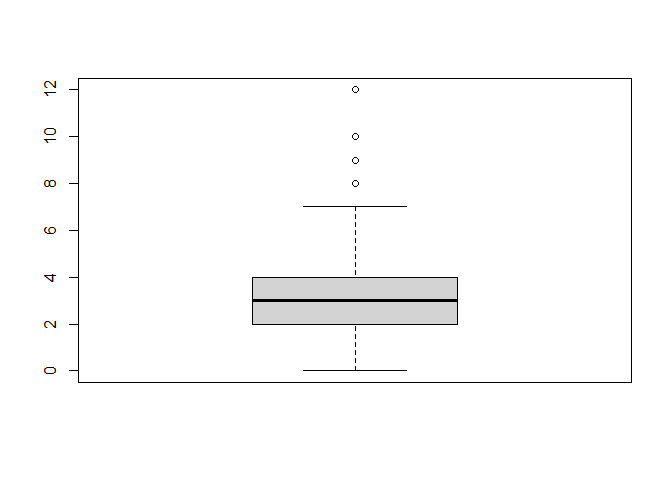
\includegraphics{OZNAL-ver2_files/figure-latex/unnamed-chunk-31-1.pdf}

\begin{Shaded}
\begin{Highlighting}[]
\FunctionTok{hist}\NormalTok{(df}\SpecialCharTok{$}\NormalTok{goals.home, }\AttributeTok{xlab=}\StringTok{"Home goals"}\NormalTok{, }\AttributeTok{main=}\StringTok{"Histogram výskytov gólov domáceho tímu"}\NormalTok{)}
\FunctionTok{abline}\NormalTok{(}\AttributeTok{v =} \FunctionTok{c}\NormalTok{(}\FunctionTok{mean}\NormalTok{(df}\SpecialCharTok{$}\NormalTok{goals.home),  }\FunctionTok{median}\NormalTok{(df}\SpecialCharTok{$}\NormalTok{goals.home)), }\AttributeTok{col=}\FunctionTok{c}\NormalTok{(}\StringTok{"green"}\NormalTok{, }\StringTok{"blue"}\NormalTok{), }\AttributeTok{lty=}\FunctionTok{c}\NormalTok{(}\DecValTok{2}\NormalTok{,}\DecValTok{3}\NormalTok{), }\AttributeTok{lwd=}\FunctionTok{c}\NormalTok{(}\DecValTok{3}\NormalTok{,}\DecValTok{3}\NormalTok{))}
\end{Highlighting}
\end{Shaded}

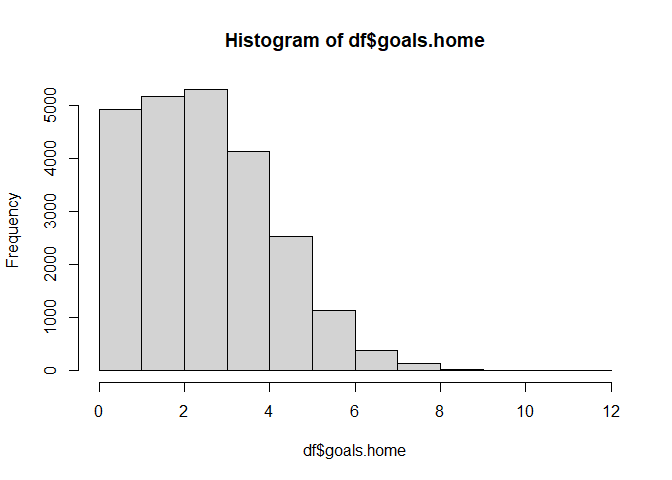
\includegraphics{OZNAL-ver2_files/figure-latex/unnamed-chunk-31-2.pdf}

\begin{Shaded}
\begin{Highlighting}[]
\FunctionTok{boxplot}\NormalTok{(df}\SpecialCharTok{$}\NormalTok{goals.away, }\AttributeTok{ylab=}\StringTok{"Away goals"}\NormalTok{, }\AttributeTok{xlab=}\StringTok{""}\NormalTok{, }\AttributeTok{main=}\StringTok{"Krabicový graf gólov hosťujúceho tímu"}\NormalTok{)}
\end{Highlighting}
\end{Shaded}

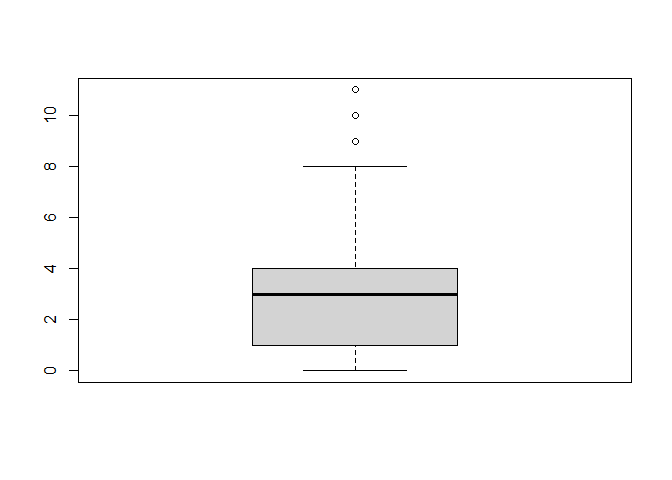
\includegraphics{OZNAL-ver2_files/figure-latex/unnamed-chunk-31-3.pdf}

\begin{Shaded}
\begin{Highlighting}[]
\FunctionTok{hist}\NormalTok{(df}\SpecialCharTok{$}\NormalTok{goals.away, }\AttributeTok{xlab=}\StringTok{"Away goals"}\NormalTok{, }\AttributeTok{main=}\StringTok{"Histogram výskytov gólov hosťujúceho tímu"}\NormalTok{)}
\FunctionTok{abline}\NormalTok{(}\AttributeTok{v =} \FunctionTok{c}\NormalTok{(}\FunctionTok{mean}\NormalTok{(df}\SpecialCharTok{$}\NormalTok{goals.home),  }\FunctionTok{median}\NormalTok{(df}\SpecialCharTok{$}\NormalTok{goals.home)), }\AttributeTok{col=}\FunctionTok{c}\NormalTok{(}\StringTok{"green"}\NormalTok{, }\StringTok{"blue"}\NormalTok{), }\AttributeTok{lty=}\FunctionTok{c}\NormalTok{(}\DecValTok{2}\NormalTok{,}\DecValTok{3}\NormalTok{), }\AttributeTok{lwd=}\FunctionTok{c}\NormalTok{(}\DecValTok{3}\NormalTok{,}\DecValTok{3}\NormalTok{))}
\end{Highlighting}
\end{Shaded}

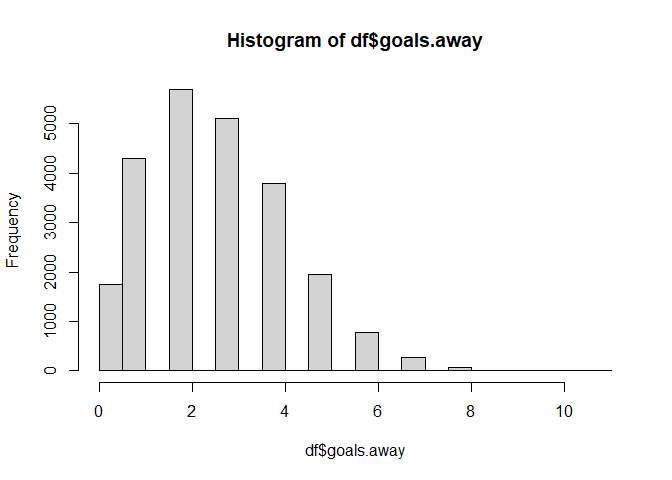
\includegraphics{OZNAL-ver2_files/figure-latex/unnamed-chunk-31-4.pdf}
Dodatočne ešte overíme, či neexistujú chýbajúce hodnoty týchto atribútov
v niektorých záznamoch:

\begin{Shaded}
\begin{Highlighting}[]
\FunctionTok{cat}\NormalTok{(}\StringTok{"Počet záznamov kde je goals.home NA"}\NormalTok{, }\FunctionTok{nrow}\NormalTok{(}\FunctionTok{subset}\NormalTok{(df, }\FunctionTok{is.na}\NormalTok{(goals.home)}\SpecialCharTok{==}\ConstantTok{TRUE}\NormalTok{)), }\StringTok{\textquotesingle{}}\SpecialCharTok{\textbackslash{}n}\StringTok{\textquotesingle{}}\NormalTok{)}
\end{Highlighting}
\end{Shaded}

\begin{verbatim}
## Počet záznamov kde je goals.home NA 0
\end{verbatim}

\begin{Shaded}
\begin{Highlighting}[]
\FunctionTok{cat}\NormalTok{(}\StringTok{"Počet záznamov kde je goals.away NA"}\NormalTok{,}\FunctionTok{nrow}\NormalTok{(}\FunctionTok{subset}\NormalTok{(df, }\FunctionTok{is.na}\NormalTok{(goals.away)}\SpecialCharTok{==}\ConstantTok{TRUE}\NormalTok{)),}\StringTok{\textquotesingle{}}\SpecialCharTok{\textbackslash{}n}\StringTok{\textquotesingle{}}\NormalTok{)}
\end{Highlighting}
\end{Shaded}

\begin{verbatim}
## Počet záznamov kde je goals.away NA 0
\end{verbatim}

Ani jeden záznam nenadobúda pri atribútoch goals.home a goals.away NA
hodnoty, preto nebude potrebné riešiť voľbu stratégie dopĺňania týchto
hodnôt.

Už z vizualizácií atribútov vidíme, že predpoklady boli korektné.
Histogramy oboch atribútov sú veľmi podobné - obe majú distribúciu
naklonenú vpravo, určite sa nebude jednať o normálne rozdelenie - z
tohoto dôvodu netreba ani vykonávať test normality. Z histogramov možno
vyčítať, že domáci tím strelí v priemere viac gólov ako hosťujúci tím -
zatiaľ čo pri hosťujúcich tímoch nadobúdajú záznamy najčastejšie hodnotu
0 gólov, pri domácich tímoch je maximálna frekvencia pri hodnote 2 góly.
Z tejto skutočnosti môžeme vyvodiť hypotézu, že domáce prostredie môže
mať reálny vplyv na priemerný počet strelených gólov, resp. vonkajšie
prostredie znižuje priemerný počet strelených gólov. Pri krabicových
grafoch možno sledovať úplnú identitu týchto grafov pre oba atribúty, čo
je zaujímavý jav, keďže histogramy sú mierne odlišné. Väčšina hodnôt sa
pohybuje v rozmedzí 2-4 góly, čiže náš počiatočný predpoklad bol
čiastočne korektný. Vychýlené hodnoty sú v oboch prípadoch počet 8, 9 a
10 gólov. Pre overenie si tieto maximálne hodnoty pre oba atribúty
vypíšeme, pričom zaujímavý bude najmä počet záznamov, ktorý tieto
hodnoty nadobúda.

\begin{Shaded}
\begin{Highlighting}[]
\FunctionTok{subset}\NormalTok{(df, goals.home }\SpecialCharTok{\textgreater{}=} \DecValTok{8}\NormalTok{)}
\end{Highlighting}
\end{Shaded}

\begin{verbatim}
##       season type goals.away goals.home team_id.away won.away shots.away
##  1: 20172018    R          3          8           22    FALSE         29
##  2: 20152016    R          1          8           22    FALSE         31
##  3: 20172018    R          4          8            5    FALSE         26
##  4: 20172018    R          3          8           24    FALSE         34
##  5: 20172018    R          1         10           17    FALSE         23
##  6: 20162017    R          4          8           19    FALSE         37
##  7: 20162017    R          7          8           15    FALSE         28
##  8: 20162017    R          2          8           25    FALSE         30
##  9: 20162017    R          6          8           23    FALSE         34
## 10: 20162017    R          1         10           21    FALSE         16
## 11: 20172018    R          3          8           19    FALSE         25
## 12: 20152016    R          3          8           20    FALSE         26
## 13: 20162017    R          5          8            9    FALSE         34
## 14: 20172018    R          2          8           15    FALSE         23
## 15: 20172018    R          5          8            3    FALSE         35
## 16: 20162017    R          0         10            8    FALSE         30
## 17: 20172018    R          1          8           12    FALSE         33
## 18: 20172018    R          2          8           54    FALSE         24
## 19: 20172018    R          2          8           20    FALSE         28
## 20: 20162017    R          3          8           24    FALSE         33
## 21: 20172018    R          1         10            5    FALSE         29
## 22: 20172018    P          1          8           24    FALSE         46
## 23: 20192020    R          2          8           26    FALSE         39
## 24: 20192020    R          4          9           18    FALSE         24
## 25: 20192020    R          2          8            9    FALSE         29
## 26: 20192020    R          3          9            3    FALSE         23
## 27: 20192020    R          6          8           23    FALSE         22
## 28: 20192020    R          6          8           12    FALSE         40
## 29: 20192020    R          2          9           23    FALSE         23
## 30: 20192020    R          4          8           10    FALSE         47
## 31: 20192020    R          2          8           17    FALSE         36
## 32: 20192020    A          5          9           88    FALSE         16
## 33: 20192020    R          3          9            6    FALSE         37
## 34: 20192020    P          2          8            2    FALSE         24
## 35: 20182019    R          5          8            3    FALSE         24
## 36: 20182019    R          2          8           17    FALSE         34
## 37: 20182019    R          2          8           29    FALSE         32
## 38: 20182019    R          3          8            1    FALSE         30
## 39: 20182019    R          2          9            9    FALSE         29
## 40: 20182019    R          5          8           28    FALSE         33
## 41: 20182019    R          5          8           16    FALSE         32
## 42: 20182019    R          5          8           15    FALSE         39
## 43: 20182019    R          3          9           24    FALSE         29
## 44: 20182019    R          3          8            1    FALSE         23
## 45: 20182019    R          7          8            9    FALSE         38
## 46: 20182019    R          2          8            8    FALSE         37
## 47: 20182019    R          4          9            1    FALSE         26
## 48: 20182019    R          4          8           26    FALSE         38
##       season type goals.away goals.home team_id.away won.away shots.away
##     hits.away pim.away powerPlayOpportunities.away powerPlayGoals.away
##  1:        32       11                           1                   0
##  2:        18       34                           1                   0
##  3:        28       19                           4                   0
##  4:        21       11                           3                   0
##  5:        36        6                           1                   0
##  6:        11       12                           5                   4
##  7:        41        4                           4                   1
##  8:        18       52                           5                   2
##  9:        15       11                           2                   0
## 10:        35        8                           3                   0
## 11:        20       12                           6                   1
## 12:        20       28                           3                   1
## 13:        51       10                           5                   3
## 14:        20       14                           2                   0
## 15:        20       12                           3                   2
## 16:        15       12                           1                   0
## 17:        22       13                           4                   0
## 18:        24        8                           4                   0
## 19:        13       67                           5                   1
## 20:        11       21                           4                   1
## 21:        38       32                           2                   1
## 22:        44       28                           3                   1
## 23:        15        4                           4                   0
## 24:        22       12                           4                   1
## 25:        30       13                           3                   0
## 26:        22       55                           4                   0
## 27:        45       10                           2                   1
## 28:        19        8                           3                   1
## 29:        18       10                           4                   0
## 30:         6        4                           3                   0
## 31:        31        4                           2                   0
## 32:         0        0                           0                   0
## 33:        29       13                           2                   1
## 34:        44       24                           5                   1
## 35:        27       12                           4                   1
## 36:        21       14                           3                   1
## 37:        20       16                           5                   0
## 38:        30       11                           3                   1
## 39:         6        8                           1                   0
## 40:        18       37                           4                   2
## 41:        10       13                           4                   1
## 42:        35       10                           2                   0
## 43:        12        8                           1                   0
## 44:        25       16                           2                   1
## 45:        16       10                           3                   1
## 46:        31        8                           6                   1
## 47:        27        2                           2                   0
## 48:        36       14                           4                   2
##     hits.away pim.away powerPlayOpportunities.away powerPlayGoals.away
##     faceOffWinPercentage.away giveaways.away takeaways.away blocked.away
##  1:                      47.5              1              9           16
##  2:                      47.7             10              6           11
##  3:                      46.9             14              9           25
##  4:                      62.3             14              4            3
##  5:                      49.2              8              7           15
##  6:                      47.5              3              2           12
##  7:                      50.0              3              5           16
##  8:                      49.2             10              5           19
##  9:                      50.0              3              9           15
## 10:                      29.8             15              4           13
## 11:                      52.0              2              3            9
## 12:                      39.7             12              5           13
## 13:                      44.6              6              7           17
## 14:                      46.7             11              6           10
## 15:                      40.3              8             15           18
## 16:                      55.6              2              1            9
## 17:                      58.5             11              5           10
## 18:                      63.5             10              6           10
## 19:                      42.3              8              1            8
## 20:                      54.5              7              6           11
## 21:                      45.1              9              7           24
## 22:                      50.0              6              4           16
## 23:                      60.9             14              3           16
## 24:                      52.9              2              9           22
## 25:                      54.3             10              9           19
## 26:                      43.3              2              3           13
## 27:                      45.2              4              2           21
## 28:                      53.3             11             17           10
## 29:                      53.4              3              2           10
## 30:                      53.5              9              6            4
## 31:                      48.9             17              5            5
## 32:                      76.2              0              2            1
## 33:                      45.5              4              6            6
## 34:                      52.7             18              8           12
## 35:                      41.5             11              8           13
## 36:                      48.5              7             14           12
## 37:                      51.7              7              6           17
## 38:                      40.3              5              7           14
## 39:                      51.6              5              1            9
## 40:                      45.5             19              7           17
## 41:                      58.3              6              5            7
## 42:                      46.8             10              6           15
## 43:                      55.9              9              2            9
## 44:                      47.5              4              3           20
## 45:                      49.2              2              8           10
## 46:                      52.9             18              7           10
## 47:                      42.4             18              6           19
## 48:                      56.1              6              5           10
##     faceOffWinPercentage.away giveaways.away takeaways.away blocked.away
##     abbreviation.away team_id.home won.home settled_in shots.home hits.home
##  1:               EDM           19     TRUE        REG         40        11
##  2:               EDM            2     TRUE        REG         31        21
##  3:               PIT            6     TRUE        REG         38        30
##  4:               ANA           13     TRUE        REG         22        12
##  5:               DET            8     TRUE        REG         34        16
##  6:               STL           29     TRUE        REG         30        20
##  7:               WSH            5     TRUE         OT         37        33
##  8:               DAL           52     TRUE        REG         31        23
##  9:               VAN           12     TRUE        REG         36        11
## 10:               COL            8     TRUE        REG         36        11
## 11:               STL           30     TRUE        REG         33        16
## 12:               CGY           24     TRUE        REG         27        15
## 13:               OTT            5     TRUE        REG         46        34
## 14:               WSH            4     TRUE        REG         37        23
## 15:               NYR           10     TRUE        REG         42        21
## 16:               MTL           29     TRUE        REG         40        12
## 17:               CAR           10     TRUE        REG         36        13
## 18:               VGK           22     TRUE        REG         32        25
## 19:               CGY           17     TRUE        REG         27        11
## 20:               ANA           20     TRUE        REG         25        13
## 21:               PIT           16     TRUE        REG         44        27
## 22:               ANA           28     TRUE        REG         36        24
## 23:               LAK           23     TRUE        REG         25        21
## 24:               NSH           21     TRUE        REG         45        16
## 25:               OTT           12     TRUE        REG         43        17
## 26:               NYR           14     TRUE        REG         45        18
## 27:               VAN            5     TRUE        REG         40        33
## 28:               CAR           10     TRUE        REG         39         4
## 29:               VAN           14     TRUE        REG         37        18
## 30:               TOR           13     TRUE        REG         29        18
## 31:               DET            2     TRUE        REG         26        27
## 32:              <NA>           87     TRUE        tbc         22         1
## 33:               BOS           23     TRUE        REG         35        31
## 34:               NYI           14     TRUE        REG         34        34
## 35:               NYR           12     TRUE        REG         40        30
## 36:               DET            6     TRUE        REG         39        21
## 37:               CBJ           14     TRUE        REG         31        22
## 38:               NJD           14     TRUE        REG         44        33
## 39:               OTT            7     TRUE        REG         41         9
## 40:               SJS           20     TRUE        REG         27        19
## 41:               CHI            1     TRUE        REG         41        21
## 42:               WSH           16     TRUE        REG         28        29
## 43:               ANA           52     TRUE        REG         31        20
## 44:               NJD           19     TRUE        REG         39         7
## 45:               OTT           16     TRUE        REG         42         4
## 46:               MTL           24     TRUE        REG         29        20
## 47:               NJD           20     TRUE        REG         39        14
## 48:               LAK           22     TRUE        REG         32        21
##     abbreviation.away team_id.home won.home settled_in shots.home hits.home
##     pim.home powerPlayOpportunities.home powerPlayGoals.home
##  1:        7                           3                   1
##  2:       18                           4                   2
##  3:       17                           5                   3
##  4:       11                           3                   1
##  5:        4                           2                   1
##  6:       18                           2                   1
##  7:       10                           1                   1
##  8:       42                           5                   3
##  9:        9                           3                   2
## 10:       10                           2                   1
## 11:       12                           6                   2
## 12:       18                           3                   1
## 13:       10                           4                   0
## 14:       14                           2                   1
## 15:        6                           6                   3
## 16:        4                           5                   4
## 17:       15                           3                   3
## 18:       10                           3                   3
## 19:       64                           6                   4
## 20:       33                           3                   2
## 21:        4                           6                   0
## 22:        8                           8                   4
## 23:        8                           2                   1
## 24:        8                           6                   2
## 25:       13                           3                   1
## 26:       37                           8                   5
## 27:        6                           4                   2
## 28:        6                           4                   2
## 29:        8                           5                   2
## 30:        6                           2                   1
## 31:        6                           1                   0
## 32:        0                           0                   0
## 33:       11                           3                   1
## 34:       12                           6                   3
## 35:       10                           4                   1
## 36:       14                           3                   1
## 37:       12                           7                   4
## 38:       11                           3                   2
## 39:        4                           3                   1
## 40:       43                           4                   1
## 41:       17                           2                   2
## 42:       10                           2                   1
## 43:        2                           4                   3
## 44:        6                           2                   0
## 45:        8                           4                   2
## 46:       12                           4                   1
## 47:        4                           1                   0
## 48:       20                           1                   1
##     pim.home powerPlayOpportunities.home powerPlayGoals.home
##     faceOffWinPercentage.home giveaways.home takeaways.home blocked.home
##  1:                      52.5              2             18            8
##  2:                      52.3             11              5            8
##  3:                      53.1              8              9            5
##  4:                      37.7             20              9           11
##  5:                      50.8             13              9           14
##  6:                      52.5              6              7           13
##  7:                      50.0              8              5           16
##  8:                      50.8             15              9           16
##  9:                      50.0             16             10           13
## 10:                      70.2             10              7           10
## 11:                      48.0             10              7           16
## 12:                      60.3             10              5           18
## 13:                      55.4              7              7           17
## 14:                      53.3             11              4           16
## 15:                      59.7             13             17            7
## 16:                      44.4              5              6           17
## 17:                      41.5             12              7           21
## 18:                      36.5             13             10           11
## 19:                      57.7              5              7           16
## 20:                      45.5             14             14           10
## 21:                      54.9             11             10           13
## 22:                      50.0             12             10           18
## 23:                      39.1              7             16           17
## 24:                      47.1             14             10           17
## 25:                      45.7             16             10           13
## 26:                      56.7              5              8           10
## 27:                      54.8             15             12           11
## 28:                      46.7             14             14           14
## 29:                      46.6              5              5           13
## 30:                      46.5             18             12           18
## 31:                      51.1             25              7           14
## 32:                      23.8              1              4            0
## 33:                      54.5             12             16           18
## 34:                      47.3             20             13           14
## 35:                      58.5             18             13           16
## 36:                      51.5              9             15            9
## 37:                      48.3             10             11           12
## 38:                      59.7              9              8           13
## 39:                      48.4              5              5           13
## 40:                      54.5             19             14           17
## 41:                      41.7              8              8           15
## 42:                      53.2              9             11           15
## 43:                      44.1             14             12           14
## 44:                      52.5              9              6            9
## 45:                      50.8              7              4           18
## 46:                      47.1             18             10           16
## 47:                      57.6             20              9            7
## 48:                      43.9              8              8           26
##     faceOffWinPercentage.home giveaways.home takeaways.home blocked.home
##     abbreviation.home save_percentage.home save_percentage.away
##  1:               STL               0.8966               0.8000
##  2:               NYI               0.9677               0.7419
##  3:               BOS               0.8462               0.7895
##  4:               FLA               0.9118               0.6364
##  5:               MTL               0.9565               0.7059
##  6:               CBJ               0.8919               0.7333
##  7:               PIT               0.7500               0.7838
##  8:               WPG               0.9333               0.7419
##  9:               CAR               0.8235               0.7778
## 10:               MTL               0.9375               0.7222
## 11:               MIN               0.8800               0.7576
## 12:               ANA               0.8846               0.7037
## 13:               PIT               0.8529               0.8261
## 14:               PHI               0.9130               0.7838
## 15:               TOR               0.8571               0.8095
## 16:               CBJ               1.0000               0.7500
## 17:               TOR               0.9697               0.7778
## 18:               EDM               0.9167               0.7500
## 19:               DET               0.9286               0.7037
## 20:               CGY               0.9091               0.6800
## 21:               CHI               0.9655               0.7727
## 22:               SJS               0.9783               0.7778
## 23:               VAN               0.9487               0.6800
## 24:               COL               0.8333               0.8000
## 25:               CAR               0.9310               0.8140
## 26:               TBL               0.8696               0.8000
## 27:               PIT               0.7273               0.8000
## 28:               TOR               0.8500               0.7949
## 29:               TBL               0.9130               0.7568
## 30:               FLA               0.9149               0.7241
## 31:               NYI               0.9444               0.6923
## 32:              <NA>               0.6875               0.5909
## 33:               VAN               0.9189               0.7429
## 34:               TBL               0.9167               0.7647
## 35:               CAR               0.7917               0.8000
## 36:               BOS               0.9412               0.7949
## 37:               TBL               0.9375               0.7419
## 38:               TBL               0.9000               0.8182
## 39:               BUF               0.9310               0.7805
## 40:               CGY               0.8485               0.7037
## 41:               NJD               0.8438               0.8049
## 42:               CHI               0.8718               0.7143
## 43:               WPG               0.8966               0.7097
## 44:               STL               0.8696               0.7949
## 45:               CHI               0.8158               0.8095
## 46:               ANA               0.9459               0.7241
## 47:               CGY               0.8462               0.7692
## 48:               EDM               0.8947               0.7500
##     abbreviation.home save_percentage.home save_percentage.away
\end{verbatim}

\begin{Shaded}
\begin{Highlighting}[]
\FunctionTok{cat}\NormalTok{(}\StringTok{"Počet vychýlených hodnôt atribútu goals.home podľa krabicového grafu:"}\NormalTok{, }\FunctionTok{nrow}\NormalTok{(}\FunctionTok{subset}\NormalTok{(df, goals.home }\SpecialCharTok{\textgreater{}=} \DecValTok{8}\NormalTok{)))}
\end{Highlighting}
\end{Shaded}

\begin{verbatim}
## Počet vychýlených hodnôt atribútu goals.home podľa krabicového grafu: 48
\end{verbatim}

\begin{Shaded}
\begin{Highlighting}[]
\FunctionTok{subset}\NormalTok{(df, goals.away }\SpecialCharTok{\textgreater{}=} \DecValTok{8}\NormalTok{)}
\end{Highlighting}
\end{Shaded}

\begin{verbatim}
##       season type goals.away goals.home team_id.away won.away shots.away
##  1: 20172018    R          8          3            1     TRUE         28
##  2: 20162017    R          8          4           12     TRUE         33
##  3: 20172018    R          8          3            8     TRUE         29
##  4: 20172018    R          8          2           16     TRUE         43
##  5: 20152016    R          9          2           26     TRUE         57
##  6: 20172018    R          8          5           14     TRUE         38
##  7: 20172018    P          8          5            5     TRUE         28
##  8: 20192020    R          8          1            6     TRUE         24
##  9: 20192020    R          8          3           18     TRUE         24
## 10: 20192020    R          8          5           30     TRUE         33
## 11: 20192020    A         10          5           90     TRUE         28
## 12: 20192020    R          8          3           22     TRUE         49
## 13: 20192020    R          8          4           16     TRUE         28
## 14: 20192020    R          8          3           22     TRUE         35
## 15: 20182019    R          8          2           28     TRUE         48
## 16: 20182019    R          9          1            5     TRUE         36
## 17: 20182019    R          8          5           23     TRUE         33
## 18: 20182019    R          8          4           52     TRUE         36
## 19: 20182019    R          8          3           54     TRUE         43
## 20: 20182019    R          9          6           20     TRUE         28
## 21: 20182019    A         10          5           88     TRUE         22
## 22: 20182019    R          8          1            8     TRUE         34
## 23: 20182019    R          8          1           52     TRUE         29
##       season type goals.away goals.home team_id.away won.away shots.away
##     hits.away pim.away powerPlayOpportunities.away powerPlayGoals.away
##  1:        34       10                           2                   1
##  2:        20        6                           2                   0
##  3:        24       21                           4                   1
##  4:        14       10                           6                   4
##  5:        30       16                           3                   3
##  6:         8       11                           5                   2
##  7:        34       10                           1                   0
##  8:        19        6                           2                   2
##  9:        24       18                           5                   2
## 10:        22       12                           2                   0
## 11:         0        0                           0                   0
## 12:        11       45                           3                   1
## 13:         6       10                           3                   0
## 14:        17        4                           1                   1
## 15:        15       12                           5                   2
## 16:        11        6                           2                   2
## 17:        15       17                           5                   2
## 18:        13       13                           5                   1
## 19:        25        4                           3                   1
## 20:        11        6                           4                   3
## 21:         0        0                           0                   0
## 22:        24       22                           0                   0
## 23:        18       10                           2                   1
##     hits.away pim.away powerPlayOpportunities.away powerPlayGoals.away
##     faceOffWinPercentage.away giveaways.away takeaways.away blocked.away
##  1:                      51.5              9              2           26
##  2:                      55.6              3              5            9
##  3:                      44.6              7              3           19
##  4:                      50.7             11              7           19
##  5:                      60.0             10             13           17
##  6:                      49.3             17             12           15
##  7:                      46.2              7              7           22
##  8:                      50.0             24              9           16
##  9:                      47.7             14              2           23
## 10:                      39.7              9              3           22
## 11:                      35.0              1              6            1
## 12:                      38.6             10              9            8
## 13:                      47.2             16             18           11
## 14:                      45.7              7              8           17
## 15:                      41.3              7              5            8
## 16:                      43.3             11              9           23
## 17:                      52.0              6             11            9
## 18:                      50.7              5              7           12
## 19:                      56.9              6             11            5
## 20:                      56.2              5              7           10
## 21:                      45.0              3              5            1
## 22:                      65.1              4              2           17
## 23:                      41.3              9             11           23
##     faceOffWinPercentage.away giveaways.away takeaways.away blocked.away
##     abbreviation.away team_id.home won.home settled_in shots.home hits.home
##  1:               NJD           54    FALSE        REG         42        28
##  2:               CAR            2    FALSE        REG         27        30
##  3:               MTL            9    FALSE        REG         28        31
##  4:               CHI            9    FALSE        REG         27        24
##  5:               LAK            6    FALSE        REG         37        30
##  6:               TBL           13    FALSE        REG         23        14
##  7:               PIT            4    FALSE        REG         26        37
##  8:               BOS            8    FALSE        REG         37        34
##  9:               NSH            2    FALSE        REG         30        34
## 10:               MIN           53    FALSE        REG         40        20
## 11:              <NA>           89    FALSE        tbc         17         0
## 12:               EDM           20    FALSE        REG         26        15
## 13:               CHI           20    FALSE        REG         42        21
## 14:               EDM           18    FALSE        REG         30        10
## 15:               SJS            4    FALSE        REG         33        21
## 16:               PIT           20    FALSE        REG         39        16
## 17:               VAN            6    FALSE        REG         28        23
## 18:               WPG           19    FALSE        REG         27        34
## 19:               VGK           16    FALSE        REG         24        17
## 20:               CGY           29    FALSE        REG         30        10
## 21:              <NA>           89    FALSE        tbc         23         0
## 22:               MTL           17    FALSE        REG         29        24
## 23:               WPG           12    FALSE        REG         29        18
##     abbreviation.away team_id.home won.home settled_in shots.home hits.home
##     pim.home powerPlayOpportunities.home powerPlayGoals.home
##  1:        4                           5                   2
##  2:        6                           2                   0
##  3:       29                           5                   2
##  4:       14                           4                   0
##  5:       16                           3                   1
##  6:       15                           3                   0
##  7:        6                           3                   0
##  8:        6                           2                   0
##  9:       34                           2                   1
## 10:        8                           4                   2
## 11:        0                           0                   0
## 12:       57                           2                   0
## 13:        8                           4                   1
## 14:        2                           2                   0
## 15:       10                           6                   2
## 16:        4                           3                   0
## 17:       27                           5                   2
## 18:       17                           3                   1
## 19:        6                           2                   0
## 20:        8                           3                   1
## 21:        0                           0                   0
## 22:       12                           5                   0
## 23:        6                           3                   0
##     pim.home powerPlayOpportunities.home powerPlayGoals.home
##     faceOffWinPercentage.home giveaways.home takeaways.home blocked.home
##  1:                      48.5             10             10            9
##  2:                      44.4             14              4           12
##  3:                      55.4              7              7           17
##  4:                      49.3             13             10           17
##  5:                      40.0              6              6           10
##  6:                      50.7             14             16           12
##  7:                      53.8             13              3           14
##  8:                      50.0             18             11           12
##  9:                      52.3             18              2           14
## 10:                      60.3              5              5           10
## 11:                      65.0              1              8            1
## 12:                      61.4             15              6           10
## 13:                      52.8             24             15           11
## 14:                      54.3             10              4           12
## 15:                      58.7             14              4            8
## 16:                      56.7              9              9           13
## 17:                      48.0             14              9           12
## 18:                      49.3              2              9           14
## 19:                      43.1              8              9           13
## 20:                      43.8             10              7            9
## 21:                      55.0              4              4            2
## 22:                      34.9             11              4           11
## 23:                      58.7             11             11            8
##     faceOffWinPercentage.home giveaways.home takeaways.home blocked.home
##     abbreviation.home save_percentage.home save_percentage.away
##  1:               VGK               0.7143               0.9286
##  2:               NYI               0.7576               0.8519
##  3:               OTT               0.7241               0.8929
##  4:               OTT               0.8140               0.9259
##  5:               BOS               0.8421               0.9459
##  6:               FLA               0.7895               0.7826
##  7:               PHI               0.7143               0.8077
##  8:               MTL               0.6667               0.9730
##  9:               NYI               0.6667               0.9000
## 10:               ARI               0.7576               0.8750
## 11:              <NA>               0.6429               0.7059
## 12:               CGY               0.8367               0.8846
## 13:               CGY               0.7143               0.9048
## 14:               NSH               0.7714               0.9000
## 15:               PHI               0.8333               0.9394
## 16:               CGY               0.7500               0.9744
## 17:               BOS               0.7576               0.8214
## 18:               STL               0.7778               0.8519
## 19:               CHI               0.8140               0.8750
## 20:               CBJ               0.6786               0.8000
## 21:              <NA>               0.5455               0.7826
## 22:               DET               0.7647               0.9655
## 23:               CAR               0.7241               0.9655
##     abbreviation.home save_percentage.home save_percentage.away
\end{verbatim}

\begin{Shaded}
\begin{Highlighting}[]
\FunctionTok{cat}\NormalTok{(}\StringTok{"Počet vychýlených hodnôt atribútu goals.away podľa krabicového grafu:"}\NormalTok{, }\FunctionTok{nrow}\NormalTok{(}\FunctionTok{subset}\NormalTok{(df, goals.away }\SpecialCharTok{\textgreater{}=} \DecValTok{8}\NormalTok{)))}
\end{Highlighting}
\end{Shaded}

\begin{verbatim}
## Počet vychýlených hodnôt atribútu goals.away podľa krabicového grafu: 23
\end{verbatim}

Z výpisov vidíme, že počet zápasov v ktorých domáci tím strelil 8 a viac
gólov je 48, zatiaľ čo počet zápasov v ktorých vonkajší tím strelil 8 a
viac gólov je 23 - tento fakt len podporuje hypotézu, že domáce
prostredie má reálny vplyv na množstvo strelených gólov. Krabicový graf
tieto hodnoty označuje ako vychýlené, no keďže obsahujú dôležité
informácie a jedná sa o reálne hodnoty (nie napr. chyby senzorov), tieto
hodnoty nie je vhodné odstraňovať a ani normovať, resp. zrážat na nižšiu
hodnotu.

V analýze atribútu budeme pokračovat prostredníctvom QQplotu, ktorý
zobrazuje odchylku od teoretického normálneho rozdelenia.

\begin{Shaded}
\begin{Highlighting}[]
\FunctionTok{qqnorm}\NormalTok{(df}\SpecialCharTok{$}\NormalTok{goals.home, }\AttributeTok{main=}\StringTok{"Q{-}Q Plot atribútu goals.home"}\NormalTok{)}
\FunctionTok{qqline}\NormalTok{(df}\SpecialCharTok{$}\NormalTok{goals.home, }\AttributeTok{col =} \StringTok{"red"}\NormalTok{, }\AttributeTok{lwd =} \DecValTok{2}\NormalTok{)}
\end{Highlighting}
\end{Shaded}

\includegraphics{OZNAL-ver2_files/figure-latex/unnamed-chunk-35-1.pdf}

\begin{Shaded}
\begin{Highlighting}[]
\FunctionTok{qqnorm}\NormalTok{(df}\SpecialCharTok{$}\NormalTok{goals.away, }\AttributeTok{main=}\StringTok{"Q{-}Q Plot atribútu goals.away"}\NormalTok{)}
\FunctionTok{qqline}\NormalTok{(df}\SpecialCharTok{$}\NormalTok{goals.away, }\AttributeTok{col =} \StringTok{"red"}\NormalTok{, }\AttributeTok{lwd =} \DecValTok{2}\NormalTok{)}
\end{Highlighting}
\end{Shaded}

\includegraphics{OZNAL-ver2_files/figure-latex/unnamed-chunk-36-1.pdf}

Ako už bolo spomínane v úvode analýzy týchto atribútov, nejedná sa o
spojité hodnoty - táto skutočnost je viditeľná aj na grafe, kedy hodnoty
atribútu \textbf{goals.home} nie sú spojité - toto správanie je
očakávané, keďže počty gólov musia byť celé čisla. Z grafov môžeme
vidieť, že počet gólov sa vychyľuje od teoretického normálneho
rozdelenia.

\begin{Shaded}
\begin{Highlighting}[]
\FunctionTok{plotNormalDensity}\NormalTok{(df}\SpecialCharTok{$}\NormalTok{goals.home, }\AttributeTok{main =} \StringTok{"Diagram hustoty atribútu goals.home"}\NormalTok{)}
\end{Highlighting}
\end{Shaded}

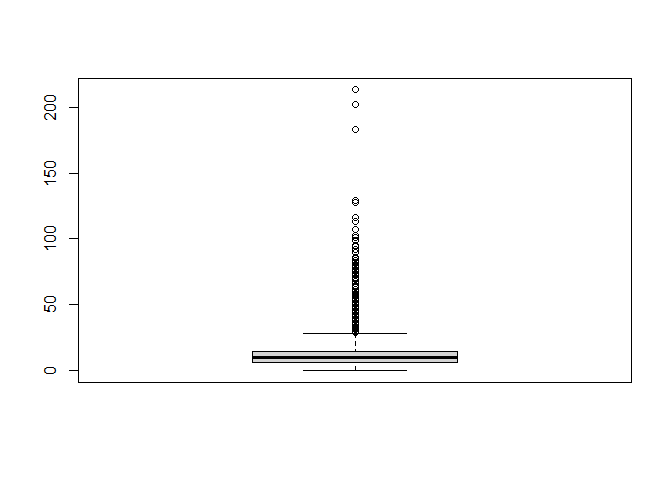
\includegraphics{OZNAL-ver2_files/figure-latex/unnamed-chunk-37-1.pdf}

\begin{Shaded}
\begin{Highlighting}[]
\FunctionTok{plotNormalDensity}\NormalTok{(df}\SpecialCharTok{$}\NormalTok{goals.away, }\AttributeTok{main =} \StringTok{"Diagram hustoty atribútu goals.away"}\NormalTok{)}
\end{Highlighting}
\end{Shaded}

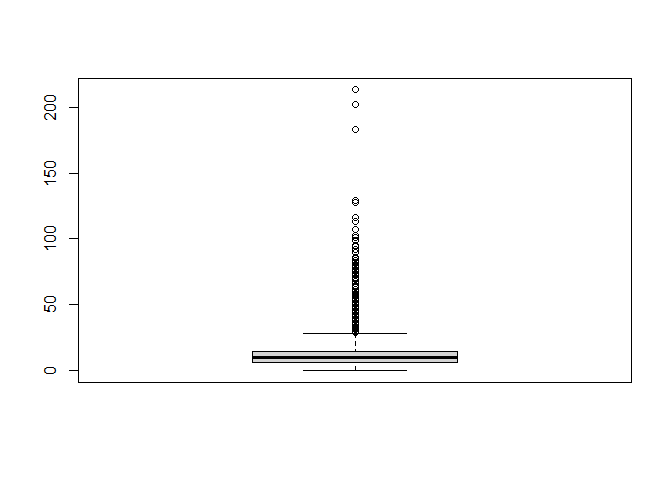
\includegraphics{OZNAL-ver2_files/figure-latex/unnamed-chunk-38-1.pdf} Z
oboch diagramov hustoty môžeme vidieť už predom spomínaný fakt -
atribúty \textbf{goals.home} a \textbf{goals.away} nepochádzajú z
normálneho rozdelenia - výrazne vychýlené od krivky hustoty normálneho
rozdelenia sú najmä hodnoty v intervale od (1-5 gólov) na x-ovej osi.
Kostrbatosť grafu spôsobuje fakt, že dáta nie sú spojité.

\begin{Shaded}
\begin{Highlighting}[]
\FunctionTok{plot}\NormalTok{(}\AttributeTok{x=}\NormalTok{df}\SpecialCharTok{$}\NormalTok{goals.home, }\AttributeTok{pch =} \DecValTok{21}\NormalTok{, }\AttributeTok{bg =} \StringTok{"lightgray"}\NormalTok{, }\AttributeTok{col =} \StringTok{"black"}\NormalTok{, }\AttributeTok{cex =} \FloatTok{0.5}\NormalTok{, }\AttributeTok{frame =} \ConstantTok{FALSE}\NormalTok{,}\AttributeTok{main =} \StringTok{"Diagram rozptýlenia atribútu goals.home"}\NormalTok{)}
\end{Highlighting}
\end{Shaded}

\includegraphics{OZNAL-ver2_files/figure-latex/unnamed-chunk-39-1.pdf}

\begin{Shaded}
\begin{Highlighting}[]
\FunctionTok{plot}\NormalTok{(df}\SpecialCharTok{$}\NormalTok{goals.away, }\AttributeTok{pch =} \DecValTok{21}\NormalTok{, }\AttributeTok{bg =} \StringTok{"lightgray"}\NormalTok{, }\AttributeTok{col =} \StringTok{"black"}\NormalTok{, }\AttributeTok{cex =} \FloatTok{0.5}\NormalTok{, }\AttributeTok{frame =} \ConstantTok{FALSE}\NormalTok{, }\AttributeTok{main =} \StringTok{"Diagram rozptýlenia atribútu goals.away"}\NormalTok{)}
\end{Highlighting}
\end{Shaded}

\includegraphics{OZNAL-ver2_files/figure-latex/unnamed-chunk-40-1.pdf} Z
grafov rozptýlenia vidieť, že podobne ako bolo viditeľné ak v krabicovom
grafe, vychýlené hodnoty sú pri počte gólov \textgreater=8 - vychýlenosť
idnikuje menšia hustota záznamov nadobúdajúcich hodnoty atribútov
\textbf{goals.home} a \textbf{goals.away} \textgreater= 8 (na grafe
viditeľné ako pomerne výrazný pokles ``bodiek''). Ako už však bolo
spomínané, odstránenie alebo úprava týchto hodnôt by so sebou niesla
riziko straty dôležitých informácií - preto bude vhodné tieto hodnoty
ponechať, keďže sa jedná o reálne údaje. Z grafu nie je príliš dobre
vidieť, pre aký počet gólov je najväčšia koncentrácia záznamov (príliš
veľa záznamov spôsobuje nízku čitateľnosť grafu) - už z krabicového
grafu však vieme, že najvyššia koncentrácia je v rozmedzí 2-4 gólov,
čiže táto informácia už nie je kľúčová.

\begin{Shaded}
\begin{Highlighting}[]
\CommentTok{\#TU NEJAKY GRAF ESTE}
\end{Highlighting}
\end{Shaded}

\textbf{Zhrnutie}: atribúty \textbf{goals.home} a \textbf{goals.away} sú
diskrétne atribúty, ktoré nepochádzajú z normálneho rozdelenia
(viditeľné na histogramoch, QQ-plotoch a grafoch hustoty), ich
distribúcia je podľa očakávaní naklonená vpravo. Z grafov rozptýlenia a
krabicových grafov vidieť, že za vychýlené hodnoty možno pri oboch
atribútoch považovať počty gólov väčšie rovné ako 8 - z dôvodu
významnosti tejto informácie však tieto hodnoty neplánujeme nijako
upravovať. Oba atribúty možno z hľadiska plánovaných hypotéz považovať
za kľúčové.

\hypertarget{atribuxfaty-team_id.home-a-team_id.away}{%
\subsubsection{Atribúty team\_id.home a
team\_id.away}\label{atribuxfaty-team_id.home-a-team_id.away}}

\textbf{charakteristika:} Identifikačné číslo NHL tímu v rámci datasetu.

Aktuálne sa v NHL nachádza 31 tímov, pričom sa tento počet od sezóny
2015/2016 nezmenil. Overíme, či sa v datatsete sedí počet tímov a
pozrieme sa aj na počet hier každého tímu, ktorý sa môže meniť pri
účasti vo vyraďovacej fáze.

\begin{Shaded}
\begin{Highlighting}[]
\FunctionTok{length}\NormalTok{(}\FunctionTok{table}\NormalTok{(df}\SpecialCharTok{$}\NormalTok{team\_id.home))}
\end{Highlighting}
\end{Shaded}

\begin{verbatim}
## [1] 34
\end{verbatim}

\begin{Shaded}
\begin{Highlighting}[]
\FunctionTok{table}\NormalTok{(df}\SpecialCharTok{$}\NormalTok{team\_id.home)}
\end{Highlighting}
\end{Shaded}

\begin{verbatim}
## 
##   1   2   3   4   5   6   7   8   9  10  12  13  14  15  16  17  18  19  20  21 
## 200 218 209 213 236 228 199 209 211 210 208 204 233 232 208 203 228 232 207 214 
##  22  23  24  25  26  28  29  30  52  53  54  87  89  90 
## 206 207 218 223 203 231 214 209 216 201 147   2   2   1
\end{verbatim}

\begin{Shaded}
\begin{Highlighting}[]
\FunctionTok{barplot}\NormalTok{(}\FunctionTok{table}\NormalTok{(df}\SpecialCharTok{$}\NormalTok{team\_id.home), }\AttributeTok{las=}\DecValTok{2}\NormalTok{, }\AttributeTok{cex.names=}\NormalTok{.}\DecValTok{8}\NormalTok{, }\AttributeTok{xlab=}\StringTok{"Frequency"}\NormalTok{, }\AttributeTok{ylab=}\StringTok{"Team ID"}\NormalTok{, }\AttributeTok{main=}\StringTok{"Počet hier pre domáce tímy"}\NormalTok{, }\AttributeTok{horiz=}\ConstantTok{TRUE}\NormalTok{, }\AttributeTok{xlim=}\FunctionTok{c}\NormalTok{(}\DecValTok{0}\NormalTok{,}\DecValTok{250}\NormalTok{), }\AttributeTok{space=}\FunctionTok{c}\NormalTok{(}\DecValTok{1}\NormalTok{,}\DecValTok{1}\NormalTok{,}\DecValTok{1}\NormalTok{,}\DecValTok{1}\NormalTok{), }\AttributeTok{col=}\FunctionTok{c}\NormalTok{(}\StringTok{"salmon2"}\NormalTok{))}
\end{Highlighting}
\end{Shaded}

\begin{verbatim}
## Warning in space + width: longer object length is not a multiple of shorter
## object length

## Warning in space + width: longer object length is not a multiple of shorter
## object length
\end{verbatim}

\includegraphics{OZNAL-ver2_files/figure-latex/unnamed-chunk-42-1.pdf}

\begin{Shaded}
\begin{Highlighting}[]
\FunctionTok{table}\NormalTok{(df}\SpecialCharTok{$}\NormalTok{team\_id.away)}
\end{Highlighting}
\end{Shaded}

\begin{verbatim}
## 
##   1   2   3   4   5   6   7   8   9  10  12  13  14  15  16  17  18  19  20  21 
## 202 219 210 212 232 225 198 206 208 214 211 203 228 233 211 201 231 233 211 217 
##  22  23  24  25  26  28  29  30  52  53  54  87  88  90 
## 210 207 212 227 205 229 215 208 212 206 141   1   3   1
\end{verbatim}

\begin{Shaded}
\begin{Highlighting}[]
\FunctionTok{barplot}\NormalTok{(}\FunctionTok{table}\NormalTok{(df}\SpecialCharTok{$}\NormalTok{team\_id.away), }\AttributeTok{las=}\DecValTok{2}\NormalTok{, }\AttributeTok{cex.names=}\NormalTok{.}\DecValTok{8}\NormalTok{, }\AttributeTok{xlab=}\StringTok{"Frequency"}\NormalTok{, }\AttributeTok{ylab=}\StringTok{"Team ID"}\NormalTok{, }\AttributeTok{main=}\StringTok{"Počet hier pre hosťujúce tímy"}\NormalTok{, }\AttributeTok{horiz=}\ConstantTok{TRUE}\NormalTok{, }\AttributeTok{xlim=}\FunctionTok{c}\NormalTok{(}\DecValTok{0}\NormalTok{,}\DecValTok{250}\NormalTok{), }\AttributeTok{space=}\FunctionTok{c}\NormalTok{(}\DecValTok{1}\NormalTok{,}\DecValTok{1}\NormalTok{,}\DecValTok{1}\NormalTok{,}\DecValTok{1}\NormalTok{), }\AttributeTok{col=}\FunctionTok{c}\NormalTok{(}\StringTok{"salmon2"}\NormalTok{))}
\end{Highlighting}
\end{Shaded}

\begin{verbatim}
## Warning in space + width: longer object length is not a multiple of shorter
## object length

## Warning in space + width: longer object length is not a multiple of shorter
## object length
\end{verbatim}

\includegraphics{OZNAL-ver2_files/figure-latex/unnamed-chunk-42-2.pdf}

Zistili sme, že v datasete je viac ako 31 tímov. Taktiež z grafov môžeme
vidieť, že niektoré tímy odohrali iba pár zápasov. Tieto zápasy si
vypíšeme nižšie. Ostatné tímy majú približne rovnaký počet zápasov
\textasciitilde(200-230).

\begin{Shaded}
\begin{Highlighting}[]
\NormalTok{df[df}\SpecialCharTok{$}\NormalTok{team\_id.away }\SpecialCharTok{\textgreater{}=} \DecValTok{55}\NormalTok{]}
\end{Highlighting}
\end{Shaded}

\begin{verbatim}
##      season type goals.away goals.home team_id.away won.away shots.away
## 1: 20192020    A          5          9           88    FALSE         16
## 2: 20192020    A         10          5           90     TRUE         28
## 3: 20192020    A          4          5           87    FALSE         11
## 4: 20182019    A          7          4           88     TRUE         26
## 5: 20182019    A         10          5           88     TRUE         22
##    hits.away pim.away powerPlayOpportunities.away powerPlayGoals.away
## 1:         0        0                           0                   0
## 2:         0        0                           0                   0
## 3:         0        0                           0                   0
## 4:         0        0                           0                   0
## 5:         0        0                           0                   0
##    faceOffWinPercentage.away giveaways.away takeaways.away blocked.away
## 1:                      76.2              0              2            1
## 2:                      35.0              1              6            1
## 3:                      37.5              2              5            2
## 4:                      56.2              2              6            1
## 5:                      45.0              3              5            1
##    abbreviation.away team_id.home won.home settled_in shots.home hits.home
## 1:              <NA>           87     TRUE        tbc         22         1
## 2:              <NA>           89    FALSE        tbc         17         0
## 3:              <NA>           90     TRUE        tbc         20         0
## 4:              <NA>           87    FALSE        tbc         20         0
## 5:              <NA>           89    FALSE        tbc         23         0
##    pim.home powerPlayOpportunities.home powerPlayGoals.home
## 1:        0                           0                   0
## 2:        0                           0                   0
## 3:        0                           0                   0
## 4:        0                           0                   0
## 5:        0                           0                   0
##    faceOffWinPercentage.home giveaways.home takeaways.home blocked.home
## 1:                      23.8              1              4            0
## 2:                      65.0              1              8            1
## 3:                      62.5              1              6            2
## 4:                      43.8              1              8            0
## 5:                      55.0              4              4            2
##    abbreviation.home save_percentage.home save_percentage.away
## 1:              <NA>               0.6875               0.5909
## 2:              <NA>               0.6429               0.7059
## 3:              <NA>               0.6364               0.7500
## 4:              <NA>               0.7308               0.8000
## 5:              <NA>               0.5455               0.7826
\end{verbatim}

Z výpisu môžeme vidieť, že tímy s nízkym počtom zápasov sú exhibičné
tímy, ktoré sme úvadzali vyššie - nejedná sa o tímy NHL. Tieto záznamy
teda bude potrebné odstrániť.

\hypertarget{atribuxfaty-won.home-a-won.away}{%
\subsubsection{Atribúty won.home a
won.away}\label{atribuxfaty-won.home-a-won.away}}

\textbf{charakteristika:} jedná sa o boolean atribúty, vyjadrujú ktorý
tím v zápase zvíťazil. V drtivej väčšine prípadov sú opačné, t.j TRUE
FALSE alebo FALSE TRUE. Môže však nastať aj situácia v ktorej majú oba
hodnotu FALSE - keďže remízy v týchto sezónach neboli povolené, tieto
hodnoty by sa reálne v datasete vyskytovať pri legitímnych záznamoch
nemali.

\begin{Shaded}
\begin{Highlighting}[]
\FunctionTok{unique}\NormalTok{(df}\SpecialCharTok{$}\NormalTok{won.home)}
\end{Highlighting}
\end{Shaded}

\begin{verbatim}
## [1]  TRUE FALSE
\end{verbatim}

\begin{Shaded}
\begin{Highlighting}[]
\FunctionTok{unique}\NormalTok{(df}\SpecialCharTok{$}\NormalTok{won.away)}
\end{Highlighting}
\end{Shaded}

\begin{verbatim}
## [1] FALSE  TRUE
\end{verbatim}

\begin{Shaded}
\begin{Highlighting}[]
\FunctionTok{subset}\NormalTok{(df, won.home}\SpecialCharTok{==}\ConstantTok{TRUE} \SpecialCharTok{\&}\NormalTok{ won.away}\SpecialCharTok{==}\ConstantTok{TRUE}\NormalTok{)}
\end{Highlighting}
\end{Shaded}

\begin{verbatim}
## Empty data.table (0 rows and 31 cols): season,type,goals.away,goals.home,team_id.away,won.away...
\end{verbatim}

\begin{Shaded}
\begin{Highlighting}[]
\FunctionTok{subset}\NormalTok{(df, won.home}\SpecialCharTok{==}\ConstantTok{FALSE} \SpecialCharTok{\&}\NormalTok{ won.away}\SpecialCharTok{==}\ConstantTok{FALSE}\NormalTok{)}
\end{Highlighting}
\end{Shaded}

\begin{verbatim}
##       season type goals.away goals.home team_id.away won.away shots.away
##  1: 20172018    P          0          0           28    FALSE          0
##  2: 20172018    P          0          0           28    FALSE         NA
##  3: 20172018    P          0          0           26    FALSE          0
##  4: 20172018    P          0          0           52    FALSE         NA
##  5: 20172018    P          0          0           54    FALSE         NA
##  6: 20172018    P          0          0           54    FALSE          0
##  7: 20172018    P          0          0           15    FALSE          0
##  8: 20172018    P          0          0            5    FALSE          0
##  9: 20162017    P          0          0           20    FALSE          0
## 10: 20162017    P          0          0           10    FALSE          0
## 11: 20162017    P          0          0           18    FALSE          0
## 12: 20162017    P          0          0           18    FALSE          0
## 13: 20162017    P          0          0           18    FALSE          0
## 14: 20162017    P          0          0            3    FALSE         NA
##     hits.away pim.away powerPlayOpportunities.away powerPlayGoals.away
##  1:         0        0                           0                   0
##  2:        NA       NA                          NA                  NA
##  3:         0        0                           0                   0
##  4:        NA       NA                          NA                  NA
##  5:        NA       NA                          NA                  NA
##  6:         0        0                           0                   0
##  7:         0        0                           0                   0
##  8:         0        0                           0                   0
##  9:         0        0                           0                   0
## 10:         0        0                           0                   0
## 11:         0        0                           0                   0
## 12:         0        0                           0                   0
## 13:         0        0                           0                   0
## 14:        NA       NA                          NA                  NA
##     faceOffWinPercentage.away giveaways.away takeaways.away blocked.away
##  1:                         0              0              0            0
##  2:                        NA             NA             NA           NA
##  3:                         0              0              0            0
##  4:                        NA             NA             NA           NA
##  5:                        NA             NA             NA           NA
##  6:                         0              0              0            0
##  7:                         0              0              0            0
##  8:                         0              0              0            0
##  9:                         0              0              0            0
## 10:                         0              0              0            0
## 11:                         0              0              0            0
## 12:                         0              0              0            0
## 13:                         0              0              0            0
## 14:                        NA             NA             NA           NA
##     abbreviation.away team_id.home won.home settled_in shots.home hits.home
##  1:               SJS           54    FALSE        tbc          0         0
##  2:               SJS           24    FALSE        tbc         NA        NA
##  3:               LAK           54    FALSE        tbc          0         0
##  4:               WPG           54    FALSE        tbc         NA        NA
##  5:               VGK           52    FALSE        tbc         NA        NA
##  6:               VGK           15    FALSE        tbc          0         0
##  7:               WSH           54    FALSE        tbc          0         0
##  8:               PIT           15    FALSE        tbc          0         0
##  9:               CGY           24    FALSE        tbc          0         0
## 10:               TOR           15    FALSE        tbc          0         0
## 11:               NSH           24    FALSE        tbc          0         0
## 12:               NSH            5    FALSE        tbc          0         0
## 13:               NSH           16    FALSE        tbc          0         0
## 14:               NYR            9    FALSE        tbc         NA        NA
##     pim.home powerPlayOpportunities.home powerPlayGoals.home
##  1:        0                           0                   0
##  2:       NA                          NA                  NA
##  3:        0                           0                   0
##  4:       NA                          NA                  NA
##  5:       NA                          NA                  NA
##  6:        0                           0                   0
##  7:        0                           0                   0
##  8:        0                           0                   0
##  9:        0                           0                   0
## 10:        0                           0                   0
## 11:        0                           0                   0
## 12:        0                           0                   0
## 13:        0                           0                   0
## 14:       NA                          NA                  NA
##     faceOffWinPercentage.home giveaways.home takeaways.home blocked.home
##  1:                         0              0              0            0
##  2:                        NA             NA             NA           NA
##  3:                         0              0              0            0
##  4:                        NA             NA             NA           NA
##  5:                        NA             NA             NA           NA
##  6:                         0              0              0            0
##  7:                         0              0              0            0
##  8:                         0              0              0            0
##  9:                         0              0              0            0
## 10:                         0              0              0            0
## 11:                         0              0              0            0
## 12:                         0              0              0            0
## 13:                         0              0              0            0
## 14:                        NA             NA             NA           NA
##     abbreviation.home save_percentage.home save_percentage.away
##  1:               VGK                  NaN                  NaN
##  2:               ANA                   NA                   NA
##  3:               VGK                  NaN                  NaN
##  4:               VGK                   NA                   NA
##  5:               WPG                   NA                   NA
##  6:               WSH                  NaN                  NaN
##  7:               VGK                  NaN                  NaN
##  8:               WSH                  NaN                  NaN
##  9:               ANA                  NaN                  NaN
## 10:               WSH                  NaN                  NaN
## 11:               ANA                  NaN                  NaN
## 12:               PIT                  NaN                  NaN
## 13:               CHI                  NaN                  NaN
## 14:               OTT                   NA                   NA
\end{verbatim}

\begin{Shaded}
\begin{Highlighting}[]
\NormalTok{verify }\OtherTok{\textless{}{-}} \FunctionTok{subset}\NormalTok{(df, won.home}\SpecialCharTok{==}\ConstantTok{FALSE} \SpecialCharTok{\&}\NormalTok{ won.away}\SpecialCharTok{==}\ConstantTok{FALSE}\NormalTok{)}
\end{Highlighting}
\end{Shaded}

Výsledok zápasu TRUE TRUE nie je možný. Preto je potrebné skontrolovať,
či sa v datasete tento výsledok nenachádza (ak áno je potrebné ho
opraviť). Po kontrole s vysužitím funkcie unique sme zistili, že TRUE
TRUE sa v datasete nachádza 0x. FALSE FALSE sa vŠak v datasete nachádza
14x - po pohľade na dáta vieme povedať, že sa nebude jednať o remízy -
pre záznamy chýbajú dáta, pravdepodobne sa bude jednať o odložené alebo
zrušené zápasy. Žiaden z týchto zápasov však pre naše riešenie nemá
pridanú hodnotu - keďže chýbajú všetky relevantné štatistické atribúty
(resp. ich hodnota je 0), tieto zápasy môžeme úplne bez problémov z
datasetu pri čistení odstrániť - nestratíme totižto žiadnu štatisticky
cennú informáciu.

\begin{Shaded}
\begin{Highlighting}[]
\FunctionTok{unique}\NormalTok{(verify}\SpecialCharTok{$}\NormalTok{season)}
\end{Highlighting}
\end{Shaded}

\begin{verbatim}
## [1] 20172018 20162017
\end{verbatim}

\begin{Shaded}
\begin{Highlighting}[]
\FunctionTok{table}\NormalTok{(}\FunctionTok{is.na}\NormalTok{(df}\SpecialCharTok{$}\NormalTok{won.home))}
\end{Highlighting}
\end{Shaded}

\begin{verbatim}
## 
## FALSE 
##  6582
\end{verbatim}

\begin{Shaded}
\begin{Highlighting}[]
\FunctionTok{table}\NormalTok{(}\FunctionTok{is.na}\NormalTok{(df}\SpecialCharTok{$}\NormalTok{won.away))}
\end{Highlighting}
\end{Shaded}

\begin{verbatim}
## 
## FALSE 
##  6582
\end{verbatim}

Atribúty won.home a won.away neobsahujú žiadne prázdne hodnoty, preto
nie je potrebné voliť stratégie ich nahrádzania.

\hypertarget{atribuxfaty-shots.home-a-shots.away}{%
\subsubsection{Atribúty shots.home a
shots.away}\label{atribuxfaty-shots.home-a-shots.away}}

\textbf{charakteristika:} atribút reprezentuje počet striel na bránu z
pohľadu domáceho a hosťovského tímu.

Pri atribútoch overíme, či neobsahujú chýbajúce hodnoty:

\begin{Shaded}
\begin{Highlighting}[]
\FunctionTok{cat}\NormalTok{(}\StringTok{"Počet záznamov kde je shots.home NA"}\NormalTok{, }\FunctionTok{nrow}\NormalTok{(}\FunctionTok{subset}\NormalTok{(df, }\FunctionTok{is.na}\NormalTok{(shots.home)}\SpecialCharTok{==}\ConstantTok{TRUE}\NormalTok{)), }\StringTok{\textquotesingle{}}\SpecialCharTok{\textbackslash{}n}\StringTok{\textquotesingle{}}\NormalTok{)}
\end{Highlighting}
\end{Shaded}

\begin{verbatim}
## Počet záznamov kde je shots.home NA 4
\end{verbatim}

\begin{Shaded}
\begin{Highlighting}[]
\FunctionTok{cat}\NormalTok{(}\StringTok{"Počet záznamov kde je shots.away NA"}\NormalTok{,}\FunctionTok{nrow}\NormalTok{(}\FunctionTok{subset}\NormalTok{(df, }\FunctionTok{is.na}\NormalTok{(shots.away)}\SpecialCharTok{==}\ConstantTok{TRUE}\NormalTok{)),}\StringTok{\textquotesingle{}}\SpecialCharTok{\textbackslash{}n}\StringTok{\textquotesingle{}}\NormalTok{)}
\end{Highlighting}
\end{Shaded}

\begin{verbatim}
## Počet záznamov kde je shots.away NA 4
\end{verbatim}

Vidíme, že v štyroch záznamoch nadobúdajú atribúty shots.home a
shots.away hodnotu NA. Na tieto záznamy sa môžeme bližšie pozrieť.

\begin{Shaded}
\begin{Highlighting}[]
\FunctionTok{subset}\NormalTok{(df, }\FunctionTok{is.na}\NormalTok{(shots.home)}\SpecialCharTok{==}\ConstantTok{TRUE}\NormalTok{)}
\end{Highlighting}
\end{Shaded}

\begin{verbatim}
##      season type goals.away goals.home team_id.away won.away shots.away
## 1: 20172018    P          0          0           28    FALSE         NA
## 2: 20172018    P          0          0           52    FALSE         NA
## 3: 20172018    P          0          0           54    FALSE         NA
## 4: 20162017    P          0          0            3    FALSE         NA
##    hits.away pim.away powerPlayOpportunities.away powerPlayGoals.away
## 1:        NA       NA                          NA                  NA
## 2:        NA       NA                          NA                  NA
## 3:        NA       NA                          NA                  NA
## 4:        NA       NA                          NA                  NA
##    faceOffWinPercentage.away giveaways.away takeaways.away blocked.away
## 1:                        NA             NA             NA           NA
## 2:                        NA             NA             NA           NA
## 3:                        NA             NA             NA           NA
## 4:                        NA             NA             NA           NA
##    abbreviation.away team_id.home won.home settled_in shots.home hits.home
## 1:               SJS           24    FALSE        tbc         NA        NA
## 2:               WPG           54    FALSE        tbc         NA        NA
## 3:               VGK           52    FALSE        tbc         NA        NA
## 4:               NYR            9    FALSE        tbc         NA        NA
##    pim.home powerPlayOpportunities.home powerPlayGoals.home
## 1:       NA                          NA                  NA
## 2:       NA                          NA                  NA
## 3:       NA                          NA                  NA
## 4:       NA                          NA                  NA
##    faceOffWinPercentage.home giveaways.home takeaways.home blocked.home
## 1:                        NA             NA             NA           NA
## 2:                        NA             NA             NA           NA
## 3:                        NA             NA             NA           NA
## 4:                        NA             NA             NA           NA
##    abbreviation.home save_percentage.home save_percentage.away
## 1:               ANA                   NA                   NA
## 2:               VGK                   NA                   NA
## 3:               WPG                   NA                   NA
## 4:               OTT                   NA                   NA
\end{verbatim}

\begin{Shaded}
\begin{Highlighting}[]
\FunctionTok{subset}\NormalTok{(df, }\FunctionTok{is.na}\NormalTok{(shots.away)}\SpecialCharTok{==}\ConstantTok{TRUE}\NormalTok{)}
\end{Highlighting}
\end{Shaded}

\begin{verbatim}
##      season type goals.away goals.home team_id.away won.away shots.away
## 1: 20172018    P          0          0           28    FALSE         NA
## 2: 20172018    P          0          0           52    FALSE         NA
## 3: 20172018    P          0          0           54    FALSE         NA
## 4: 20162017    P          0          0            3    FALSE         NA
##    hits.away pim.away powerPlayOpportunities.away powerPlayGoals.away
## 1:        NA       NA                          NA                  NA
## 2:        NA       NA                          NA                  NA
## 3:        NA       NA                          NA                  NA
## 4:        NA       NA                          NA                  NA
##    faceOffWinPercentage.away giveaways.away takeaways.away blocked.away
## 1:                        NA             NA             NA           NA
## 2:                        NA             NA             NA           NA
## 3:                        NA             NA             NA           NA
## 4:                        NA             NA             NA           NA
##    abbreviation.away team_id.home won.home settled_in shots.home hits.home
## 1:               SJS           24    FALSE        tbc         NA        NA
## 2:               WPG           54    FALSE        tbc         NA        NA
## 3:               VGK           52    FALSE        tbc         NA        NA
## 4:               NYR            9    FALSE        tbc         NA        NA
##    pim.home powerPlayOpportunities.home powerPlayGoals.home
## 1:       NA                          NA                  NA
## 2:       NA                          NA                  NA
## 3:       NA                          NA                  NA
## 4:       NA                          NA                  NA
##    faceOffWinPercentage.home giveaways.home takeaways.home blocked.home
## 1:                        NA             NA             NA           NA
## 2:                        NA             NA             NA           NA
## 3:                        NA             NA             NA           NA
## 4:                        NA             NA             NA           NA
##    abbreviation.home save_percentage.home save_percentage.away
## 1:               ANA                   NA                   NA
## 2:               VGK                   NA                   NA
## 3:               WPG                   NA                   NA
## 4:               OTT                   NA                   NA
\end{verbatim}

Z výpisu vidíme, že v oboch prípadoch sa jedná o zápasy play-off medzi
tímami NHL, ktoré vŠak neobsahujú žiade štatistické informácie (takmer
všetko je NA) - tieto záznamy bude vhodné odstrániť, keďže neobsahujú
žiadne relevantné informácie, pravdepodobne sa jedná o zrušené zápasy v
play-off. Taktiež je vhodné podotknúť, že tieto 4 zápasy sú rovnaké pre
oba atribúty, t.j. po ich odstránení budú odstránené NA hodnoty pre oba
atribúty - bude riešené vo fázi čistenia dát.

\begin{Shaded}
\begin{Highlighting}[]
\FunctionTok{boxplot}\NormalTok{(df}\SpecialCharTok{$}\NormalTok{shots.home, }\AttributeTok{ylab=}\StringTok{"Home shots"}\NormalTok{, }\AttributeTok{xlab=}\StringTok{""}\NormalTok{, }\AttributeTok{main=}\StringTok{"Krabicový graf striel na bránu domáceho tímu"}\NormalTok{)}
\end{Highlighting}
\end{Shaded}

\includegraphics{OZNAL-ver2_files/figure-latex/unnamed-chunk-49-1.pdf}

\begin{Shaded}
\begin{Highlighting}[]
\FunctionTok{hist}\NormalTok{(df}\SpecialCharTok{$}\NormalTok{shots.home, }\AttributeTok{xlab=}\StringTok{"Home shots"}\NormalTok{, }\AttributeTok{main=}\StringTok{"Histogram striel na bránu domáceho tímu"}\NormalTok{)}
\end{Highlighting}
\end{Shaded}

\includegraphics{OZNAL-ver2_files/figure-latex/unnamed-chunk-49-2.pdf}

\begin{Shaded}
\begin{Highlighting}[]
\FunctionTok{boxplot}\NormalTok{(df}\SpecialCharTok{$}\NormalTok{shots.away, }\AttributeTok{ylab=}\StringTok{"Away shots"}\NormalTok{, }\AttributeTok{xlab=}\StringTok{""}\NormalTok{, }\AttributeTok{main=}\StringTok{"Krabicový graf striel na bránu hosťujúceho tímu"}\NormalTok{)}
\end{Highlighting}
\end{Shaded}

\includegraphics{OZNAL-ver2_files/figure-latex/unnamed-chunk-49-3.pdf}

\begin{Shaded}
\begin{Highlighting}[]
\FunctionTok{hist}\NormalTok{(df}\SpecialCharTok{$}\NormalTok{shots.away, }\AttributeTok{xlab=}\StringTok{"Away shots"}\NormalTok{, }\AttributeTok{main=}\StringTok{"Histogram striel na bránu hosťujúceho tímu"}\NormalTok{)}
\end{Highlighting}
\end{Shaded}

\includegraphics{OZNAL-ver2_files/figure-latex/unnamed-chunk-49-4.pdf}

Z histogramov možno vidieť, že distribúcia atribútov shots.home a
shots.away pripomína normálnu distribúciu. Taktiež možno sledovať
odlahľú hodnotu - konkrétne počet striel 0. Ako sme už zistili, jedná sa
o chýbajúce záznamy, ktoré budú neskôr odstránené. Predpokladáme teda,
že táto odľahlá hodnota bude po fáze čistenia dát eliminovaná. Ohľadom
hodnôt atribútov vieme povedať, že aj pri \textbf{shots.home} aj
\textbf{shots.away} nadobúdajú atribúty veľmi podobné hodnoty -
najväčšia koncentrácia záznamov je okolo 30 striel. Pri prvom pohľade na
histogram však vyzerá, že hosťujúce tímy mávajú v priemere o niečo málo
viac striel na bránu ako domáce, čo je zaujímavé, keďže domáce tímy
mávajú priemerne viac gólov na zápas (ako bolo opísané v analýze
atribútov \textbf{goals.home} a \textbf{goals.away}).

Pri krabicových grafoch je zaujímavý najmä atribút \textbf{shots.home} -
konkrétne pomerne výrazne odľahlá hodnota okolo 80 striel na bránu
(najbližšia druhá je okolo 60 striel). Pri atribúte \textbf{shots.away}
- sú všetky ``odľahlé'' hodnoty združené okolo hodnoty 60 striel. Počet
80+ striel teda na prvý pohľad pôsobí podozrivo - tento záznam si
vypíšeme aby sme zistili, či sa môže jednať o chybu merania. Odľahlá
hodnota je taktiež hodnota 0, dôvod jej výskytu + postup riešenia sme
však už riešili pri opise histogramu.

\begin{Shaded}
\begin{Highlighting}[]
\FunctionTok{subset}\NormalTok{(df, df}\SpecialCharTok{$}\NormalTok{shots.home }\SpecialCharTok{\textgreater{}=} \DecValTok{80}\NormalTok{)}
\end{Highlighting}
\end{Shaded}

\begin{verbatim}
##      season type goals.away goals.home team_id.away won.away shots.away
## 1: 20192020    P          2          3           29    FALSE         63
##    hits.away pim.away powerPlayOpportunities.away powerPlayGoals.away
## 1:        46        8                           5                   1
##    faceOffWinPercentage.away giveaways.away takeaways.away blocked.away
## 1:                      47.8             21             18           62
##    abbreviation.away team_id.home won.home settled_in shots.home hits.home
## 1:               CBJ           14     TRUE         OT         88        59
##    pim.home powerPlayOpportunities.home powerPlayGoals.home
## 1:       10                           4                   0
##    faceOffWinPercentage.home giveaways.home takeaways.home blocked.home
## 1:                      52.2             28             13           30
##    abbreviation.home save_percentage.home save_percentage.away
## 1:               TBL               0.9683               0.9659
\end{verbatim}

Z výpisu záznamu vidíme, že sa jedná o zápas play-off medzi Columbus
Blue Jackets a Tamba Bay Lightning, kedy bol počet striel na jednej
strane 88 a na druhej 63. Zápas bol taktiež ukončený v predĺžení - keďže
v play-off je možný nekonečný počet predĺžení až pokiaľ nie je jasný
výsledok zápasu (remíza vo vyraďovacích zápasoch nie je povolená) môžeme
predpokladať, že sa jedná o zápas ktorý bol predĺžovaný viac krát. Počty
striel sú teda legitímne a nejedná sa o chyby merania. Jedná sa však o
veľmi unikátnu situáciu, ktorá môže potenciálne negatívne ovplyvniť
výsledky predikčného modelu. Z tohoto dôvôdu je vhodné uvažovať nad
normovaním tejto hodnoty.

\begin{Shaded}
\begin{Highlighting}[]
\FunctionTok{qqnorm}\NormalTok{(df}\SpecialCharTok{$}\NormalTok{shots.home, }\AttributeTok{main=}\StringTok{"Q{-}Q Plot atribútu shots.home"}\NormalTok{)}
\FunctionTok{qqline}\NormalTok{(df}\SpecialCharTok{$}\NormalTok{shots.home, }\AttributeTok{col =} \StringTok{"red"}\NormalTok{, }\AttributeTok{lwd =} \DecValTok{2}\NormalTok{)}
\end{Highlighting}
\end{Shaded}

\includegraphics{OZNAL-ver2_files/figure-latex/unnamed-chunk-51-1.pdf} Z
QQ-plotu atribútu \textbf{shots.home} môžeme vidieť, že sa pomerne pekne
drží teoretickej krivky normálneho rozdelenia. Síce sa jedná o diskrétnu
celočíselnú hodnotu, graf nie je taký kostrbatý ako pri atribútoch
\textbf{goals.home} a \textbf{goals.away} - je tomu tak preto, že
atribút shots dosahuje širší interval hodnôt a tým pádom na grafe skoky
medzi hodnotami nie je vidieť. Okolo počtu gólov 3 sa začína rozdelenie
mierne odchylovať od krivky normálneho rozdelenia. Za zmienku stoja aj
vychýlené hodnoty v 0 (už opísané aj zdôvodnené) a výrazne vychýlená
hodnota 80 - jedná sa o reálnu hodnotu, no nad jej normalizáciou budeme
uvažovať keďže situáciu, v ktorej hodnota bola nadobudnutá je možno
považovať za extremálnu.

\begin{Shaded}
\begin{Highlighting}[]
\FunctionTok{qqnorm}\NormalTok{(df}\SpecialCharTok{$}\NormalTok{shots.away, }\AttributeTok{main=}\StringTok{"Q{-}Q Plot atribútu shots.away"}\NormalTok{)}
\FunctionTok{qqline}\NormalTok{(df}\SpecialCharTok{$}\NormalTok{shots.away, }\AttributeTok{col =} \StringTok{"red"}\NormalTok{, }\AttributeTok{lwd =} \DecValTok{2}\NormalTok{)}
\end{Highlighting}
\end{Shaded}

\includegraphics{OZNAL-ver2_files/figure-latex/unnamed-chunk-52-1.pdf}
Pri QQ-plote atribútu \textbf{shots.away} vieme poznamenať v podstate to
isté ako pri atribúte \textbf{shots.home}. Rozdielom však je pomerne
prudšie vychýlenie od teoretickej krivky normálneho rozdelenia pre pri
počte striel väčšom rovnom ako 40. Výrazne vychýlená hodnota ako v
predošlom grafe tu však nie je, všetky nadobúdajú hodnoty okolo 60 (bolo
viditeľné už z krabicového grafu). Vyzerá to však tak, že distribúcia
normálna nebude a bude potrebná normalizácia atribútu tak, aby sme
normálne rozdelenie dosiahli.

\begin{Shaded}
\begin{Highlighting}[]
\FunctionTok{plotNormalDensity}\NormalTok{(df}\SpecialCharTok{$}\NormalTok{shots.home, }\AttributeTok{main =} \StringTok{"Diagram hustoty atribútu shots.home"}\NormalTok{)}
\end{Highlighting}
\end{Shaded}

\includegraphics{OZNAL-ver2_files/figure-latex/unnamed-chunk-53-1.pdf}

\begin{Shaded}
\begin{Highlighting}[]
\FunctionTok{plotNormalDensity}\NormalTok{(df}\SpecialCharTok{$}\NormalTok{shots.away, }\AttributeTok{main =} \StringTok{"Diagram hustoty atribútu shots.away"}\NormalTok{)}
\end{Highlighting}
\end{Shaded}

\includegraphics{OZNAL-ver2_files/figure-latex/unnamed-chunk-54-1.pdf}
Grafy hustoty indikujú takmer ideálnu hustotu atribútov
\textbf{shots.home} a \textbf{shots.away} - vyzerá to tak, že atribúty
budú mať normálnu distribúciu. Z predošlých grafov však máme dôvod o
tejto skutočnosti pochybovať, bude teda pravdepodobne potrebné vykonať
test normality na reprezentatívnej vzorke dát o veľkosti 1000.

\begin{Shaded}
\begin{Highlighting}[]
\FunctionTok{plot}\NormalTok{(}\AttributeTok{x=}\NormalTok{df}\SpecialCharTok{$}\NormalTok{shots.home, }\AttributeTok{pch =} \DecValTok{21}\NormalTok{, }\AttributeTok{bg =} \StringTok{"lightgray"}\NormalTok{, }\AttributeTok{col =} \StringTok{"black"}\NormalTok{, }\AttributeTok{cex =} \FloatTok{0.5}\NormalTok{, }\AttributeTok{frame =} \ConstantTok{FALSE}\NormalTok{,}\AttributeTok{main =} \StringTok{"Diagram rozptýlenia atribútu shots.home"}\NormalTok{)}
\end{Highlighting}
\end{Shaded}

\includegraphics{OZNAL-ver2_files/figure-latex/unnamed-chunk-55-1.pdf}
Diagram rozptýlenia atribútu \textbf{shots.home} indikuje primánrne
zoskupenie hodnôt v intervale od 20-40 striel na bránu, rovnako ako
krabicový graf. Opätovne môžeme vidieť extrémnu vychýlenosť hodnoty 88
striel na bránu. Hodnoty 0 sú chýbajúce záznamy, vyjadrovať sa k nim
teda nie je potrebné.

\begin{Shaded}
\begin{Highlighting}[]
\FunctionTok{plot}\NormalTok{(}\AttributeTok{x=}\NormalTok{df}\SpecialCharTok{$}\NormalTok{shots.away, }\AttributeTok{pch =} \DecValTok{21}\NormalTok{, }\AttributeTok{bg =} \StringTok{"lightgray"}\NormalTok{, }\AttributeTok{col =} \StringTok{"black"}\NormalTok{, }\AttributeTok{cex =} \FloatTok{0.5}\NormalTok{, }\AttributeTok{frame =} \ConstantTok{FALSE}\NormalTok{,}\AttributeTok{main =} \StringTok{"Diagram rozptýlenia atribútu shots.away"}\NormalTok{)}
\end{Highlighting}
\end{Shaded}

\includegraphics{OZNAL-ver2_files/figure-latex/unnamed-chunk-56-1.pdf}
Diagram rozptýlenia atribútu \textbf{shots.away} indikuje opäť primárne
zoskupenie hodnôt v intervale od 20-40 striel na bránu, rovnako ako
predošlý graf rozptýlenia. Neexistuje extrémne vychýlená hodnota, tým
pádom je os Y grafu posunutá. Údaje získané z grafov však vyzerajú v
oboch atribútoch veľmi podobne.

Grafy indikujú signifikantnú podobnosť s normálnym rozdelením. Bude
preto vhodné vykonať Shapiro-Wilkov test normality, pre ktorý je
potrebné vybrať reprezentatívnu vzorku o veľkosti 1000.

\begin{Shaded}
\begin{Highlighting}[]
\NormalTok{sample }\OtherTok{\textless{}{-}} \FunctionTok{sample\_n}\NormalTok{(df, }\DecValTok{1000}\NormalTok{)}
\FunctionTok{hist}\NormalTok{(sample}\SpecialCharTok{$}\NormalTok{shots.home, }\AttributeTok{xlab=}\StringTok{"Home shots"}\NormalTok{, }\AttributeTok{main=}\StringTok{"Histogram reprezentatívnej vzorky striel na bránu hosťujúceho tímu"}\NormalTok{)}
\end{Highlighting}
\end{Shaded}

\includegraphics{OZNAL-ver2_files/figure-latex/unnamed-chunk-57-1.pdf}

\begin{Shaded}
\begin{Highlighting}[]
\FunctionTok{hist}\NormalTok{(sample}\SpecialCharTok{$}\NormalTok{shots.away, }\AttributeTok{xlab=}\StringTok{"Away shots"}\NormalTok{, }\AttributeTok{main=}\StringTok{"Histogram reprezentatívnej vzorky striel na bránu hosťujúceho tímu"}\NormalTok{)}
\end{Highlighting}
\end{Shaded}

\includegraphics{OZNAL-ver2_files/figure-latex/unnamed-chunk-57-2.pdf}

\begin{Shaded}
\begin{Highlighting}[]
\FunctionTok{cat}\NormalTok{(}\StringTok{"Štatistika shots.home}\SpecialCharTok{\textbackslash{}n}\StringTok{"}\NormalTok{)}
\end{Highlighting}
\end{Shaded}

\begin{verbatim}
## Štatistika shots.home
\end{verbatim}

\begin{Shaded}
\begin{Highlighting}[]
\FunctionTok{summary}\NormalTok{(df}\SpecialCharTok{$}\NormalTok{shots.home)}
\end{Highlighting}
\end{Shaded}

\begin{verbatim}
##    Min. 1st Qu.  Median    Mean 3rd Qu.    Max.    NA's 
##    0.00   27.00   31.00   31.63   36.00   88.00       4
\end{verbatim}

\begin{Shaded}
\begin{Highlighting}[]
\FunctionTok{cat}\NormalTok{(}\StringTok{"Štatistika vzorky shots.home}\SpecialCharTok{\textbackslash{}n}\StringTok{"}\NormalTok{)}
\end{Highlighting}
\end{Shaded}

\begin{verbatim}
## Štatistika vzorky shots.home
\end{verbatim}

\begin{Shaded}
\begin{Highlighting}[]
\FunctionTok{summary}\NormalTok{(sample}\SpecialCharTok{$}\NormalTok{shots.home)}
\end{Highlighting}
\end{Shaded}

\begin{verbatim}
##    Min. 1st Qu.  Median    Mean 3rd Qu.    Max.    NA's 
##    0.00   27.00   32.00   31.73   36.00   64.00       1
\end{verbatim}

\begin{Shaded}
\begin{Highlighting}[]
\FunctionTok{cat}\NormalTok{(}\StringTok{"Štatistika shots.away}\SpecialCharTok{\textbackslash{}n}\StringTok{"}\NormalTok{)}
\end{Highlighting}
\end{Shaded}

\begin{verbatim}
## Štatistika shots.away
\end{verbatim}

\begin{Shaded}
\begin{Highlighting}[]
\FunctionTok{summary}\NormalTok{(df}\SpecialCharTok{$}\NormalTok{shots.away)}
\end{Highlighting}
\end{Shaded}

\begin{verbatim}
##    Min. 1st Qu.  Median    Mean 3rd Qu.    Max.    NA's 
##    0.00   26.00   30.00   30.19   34.00   63.00       4
\end{verbatim}

\begin{Shaded}
\begin{Highlighting}[]
\FunctionTok{cat}\NormalTok{(}\StringTok{"Štatistika vzorky shots.away}\SpecialCharTok{\textbackslash{}n}\StringTok{"}\NormalTok{)}
\end{Highlighting}
\end{Shaded}

\begin{verbatim}
## Štatistika vzorky shots.away
\end{verbatim}

\begin{Shaded}
\begin{Highlighting}[]
\FunctionTok{summary}\NormalTok{(sample}\SpecialCharTok{$}\NormalTok{shots.away)}
\end{Highlighting}
\end{Shaded}

\begin{verbatim}
##    Min. 1st Qu.  Median    Mean 3rd Qu.    Max.    NA's 
##    0.00   25.00   30.00   30.57   35.00   62.00       1
\end{verbatim}

Zo základnej deskriptívnej štatistiky možno vidieť veľmi podobnú
varianciu hodnôt vo vzorkách (dolný-horný kvantil, priemer a medián),
preto ich považujeme za reprezentatívne (aj keď neobsahujú všetky
extremálne hodnoty).

Následne vykonáme už predom spomínaný Shapiro-Wilkov test normality s
hladinou p = 0.05.

Test normality atribútu \textbf{shots.home}: nulová hypotéza: dáta
pochádzajú z normálneho rozdelenia

\begin{Shaded}
\begin{Highlighting}[]
\FunctionTok{shapiro.test}\NormalTok{(sample}\SpecialCharTok{$}\NormalTok{shots.home)}
\end{Highlighting}
\end{Shaded}

\begin{verbatim}
## 
##  Shapiro-Wilk normality test
## 
## data:  sample$shots.home
## W = 0.98876, p-value = 6.241e-07
\end{verbatim}

Keďže p \textless{} 0.05, nulovú hypotézu zamietame - dáta nepochádzajú
z normálneho rozdelenia

Test normality atribútu \textbf{shots.away}: nulová hypotéza: dáta
pochádzajú z normálneho rozdelenia

\begin{Shaded}
\begin{Highlighting}[]
\FunctionTok{shapiro.test}\NormalTok{(sample}\SpecialCharTok{$}\NormalTok{shots.away)}
\end{Highlighting}
\end{Shaded}

\begin{verbatim}
## 
##  Shapiro-Wilk normality test
## 
## data:  sample$shots.away
## W = 0.98895, p-value = 7.732e-07
\end{verbatim}

Keďže p \textless{} 0.05, nulovú hypotézu zamietame - dáta nepochádzajú
z normálneho rozdelenia.

Test normality bol v pri oboch atribútoch zamietnutý, preto vieme, že
ani jeden atribút nepochádza z normálneho rozdelenia - pravdepodobná je
mierna asymteria distribúcií atribútov.

\textbf{Zhrnutie}: atribúty \textbf{shots.home} a \textbf{shots.away} sú
diskrétne atribúty, ktoré nepochádzajú z normálneho rozdelenia (dokázané
Shapiro-Wilkovým testom). Hodnota \textbf{shots.home} dosahuje výrazne
vychýlenú hodnotu 88, pri ktorej však bola zistená jej validita (t.j.
jedná sa o valídnu hodnotu a nie chybu senzora). Túto hodnotu
pravdepodobne bude vhodné normalizovať napr. pomocou horného kvantilu,
keďže je naozaj extremálna. Atribúty \textbf{shots.home} a
\textbf{shots.away} sú na grafov veľmi podobné, dosahujú miernu
asymetriu. Vychýlené hodnoty 0 sa vyskytujú v oboch atribútoch, bolo
však zistené, že sa jedná o chýbajúce záznamy (zrušené/presunuté zápasy)
- tie budú vyriešené pri fáze čistenia dát.

\hypertarget{atribuxfaty-hits.home-a-hits.away}{%
\subsubsection{Atribúty hits.home a
hits.away}\label{atribuxfaty-hits.home-a-hits.away}}

\textbf{charakteristika:} atribút obsahuje hodnoty počtu narazení
domáceho a hosťujúceho tímu. Narazenia, resp. osobné súboje vznikajú
počas hry a pripočítavajú sa na stranu tímu, ktorý narazenie inicioval.
Preto sa hodnoty medzi súperiacimi tímami nemusia rovnať.

\begin{Shaded}
\begin{Highlighting}[]
\FunctionTok{summary}\NormalTok{(df}\SpecialCharTok{$}\NormalTok{hits.home)}
\end{Highlighting}
\end{Shaded}

\begin{verbatim}
##    Min. 1st Qu.  Median    Mean 3rd Qu.    Max.    NA's 
##    0.00   18.00   23.00   23.43   28.00   80.00       4
\end{verbatim}

\begin{Shaded}
\begin{Highlighting}[]
\FunctionTok{summary}\NormalTok{(df}\SpecialCharTok{$}\NormalTok{hits.away)}
\end{Highlighting}
\end{Shaded}

\begin{verbatim}
##    Min. 1st Qu.  Median    Mean 3rd Qu.    Max.    NA's 
##    0.00   16.00   21.00   22.44   27.00   80.00       4
\end{verbatim}

Zo zhrnutia môžeme vidieť, že hodnoty môžu byť pravdivé, resp.
neobsahujú čísla, ktoré by logicky nemohli nastať. Taktiež vidíme, že v
štyroch záznamoch nám chýbajú hodnoty tohoto atribútu.

\begin{Shaded}
\begin{Highlighting}[]
\NormalTok{df[}\FunctionTok{is.na}\NormalTok{(df}\SpecialCharTok{$}\NormalTok{hits.home)]}
\end{Highlighting}
\end{Shaded}

\begin{verbatim}
##      season type goals.away goals.home team_id.away won.away shots.away
## 1: 20172018    P          0          0           28    FALSE         NA
## 2: 20172018    P          0          0           52    FALSE         NA
## 3: 20172018    P          0          0           54    FALSE         NA
## 4: 20162017    P          0          0            3    FALSE         NA
##    hits.away pim.away powerPlayOpportunities.away powerPlayGoals.away
## 1:        NA       NA                          NA                  NA
## 2:        NA       NA                          NA                  NA
## 3:        NA       NA                          NA                  NA
## 4:        NA       NA                          NA                  NA
##    faceOffWinPercentage.away giveaways.away takeaways.away blocked.away
## 1:                        NA             NA             NA           NA
## 2:                        NA             NA             NA           NA
## 3:                        NA             NA             NA           NA
## 4:                        NA             NA             NA           NA
##    abbreviation.away team_id.home won.home settled_in shots.home hits.home
## 1:               SJS           24    FALSE        tbc         NA        NA
## 2:               WPG           54    FALSE        tbc         NA        NA
## 3:               VGK           52    FALSE        tbc         NA        NA
## 4:               NYR            9    FALSE        tbc         NA        NA
##    pim.home powerPlayOpportunities.home powerPlayGoals.home
## 1:       NA                          NA                  NA
## 2:       NA                          NA                  NA
## 3:       NA                          NA                  NA
## 4:       NA                          NA                  NA
##    faceOffWinPercentage.home giveaways.home takeaways.home blocked.home
## 1:                        NA             NA             NA           NA
## 2:                        NA             NA             NA           NA
## 3:                        NA             NA             NA           NA
## 4:                        NA             NA             NA           NA
##    abbreviation.home save_percentage.home save_percentage.away
## 1:               ANA                   NA                   NA
## 2:               VGK                   NA                   NA
## 3:               WPG                   NA                   NA
## 4:               OTT                   NA                   NA
\end{verbatim}

\begin{Shaded}
\begin{Highlighting}[]
\NormalTok{df[}\FunctionTok{is.na}\NormalTok{(df}\SpecialCharTok{$}\NormalTok{hits.away)]}
\end{Highlighting}
\end{Shaded}

\begin{verbatim}
##      season type goals.away goals.home team_id.away won.away shots.away
## 1: 20172018    P          0          0           28    FALSE         NA
## 2: 20172018    P          0          0           52    FALSE         NA
## 3: 20172018    P          0          0           54    FALSE         NA
## 4: 20162017    P          0          0            3    FALSE         NA
##    hits.away pim.away powerPlayOpportunities.away powerPlayGoals.away
## 1:        NA       NA                          NA                  NA
## 2:        NA       NA                          NA                  NA
## 3:        NA       NA                          NA                  NA
## 4:        NA       NA                          NA                  NA
##    faceOffWinPercentage.away giveaways.away takeaways.away blocked.away
## 1:                        NA             NA             NA           NA
## 2:                        NA             NA             NA           NA
## 3:                        NA             NA             NA           NA
## 4:                        NA             NA             NA           NA
##    abbreviation.away team_id.home won.home settled_in shots.home hits.home
## 1:               SJS           24    FALSE        tbc         NA        NA
## 2:               WPG           54    FALSE        tbc         NA        NA
## 3:               VGK           52    FALSE        tbc         NA        NA
## 4:               NYR            9    FALSE        tbc         NA        NA
##    pim.home powerPlayOpportunities.home powerPlayGoals.home
## 1:       NA                          NA                  NA
## 2:       NA                          NA                  NA
## 3:       NA                          NA                  NA
## 4:       NA                          NA                  NA
##    faceOffWinPercentage.home giveaways.home takeaways.home blocked.home
## 1:                        NA             NA             NA           NA
## 2:                        NA             NA             NA           NA
## 3:                        NA             NA             NA           NA
## 4:                        NA             NA             NA           NA
##    abbreviation.home save_percentage.home save_percentage.away
## 1:               ANA                   NA                   NA
## 2:               VGK                   NA                   NA
## 3:               WPG                   NA                   NA
## 4:               OTT                   NA                   NA
\end{verbatim}

Väčšina zo záznamov s chýbajúcimi hodnotami, je z jednej sezóny. Vyzerá
to ako preložené, alebo zrušené zápasy a budeme sa na to musieť pozrieť.

\begin{Shaded}
\begin{Highlighting}[]
\FunctionTok{hist}\NormalTok{(df}\SpecialCharTok{$}\NormalTok{hits.home, }\AttributeTok{xlab=}\StringTok{"Home hits"}\NormalTok{, }\AttributeTok{main=}\StringTok{"Histogram hitov domáceho tímu"}\NormalTok{)}
\end{Highlighting}
\end{Shaded}

\includegraphics{OZNAL-ver2_files/figure-latex/unnamed-chunk-62-1.pdf}

\begin{Shaded}
\begin{Highlighting}[]
\FunctionTok{hist}\NormalTok{(df}\SpecialCharTok{$}\NormalTok{hits.away, }\AttributeTok{xlab=}\StringTok{"Away hits"}\NormalTok{, }\AttributeTok{main=}\StringTok{"Histogram hitov hosťujúceho tímu"}\NormalTok{)}
\end{Highlighting}
\end{Shaded}

\includegraphics{OZNAL-ver2_files/figure-latex/unnamed-chunk-62-2.pdf}
Diagram pripomína normálne rozdelenie hodnôt, ale obsahuje niekoľko
vychýlených hodnôt, ktoré mohli nastať z dôvodu dlhších zápasov, napr.
predĺženia. Pre tento atribút bude vhodné vykonať Shapiro-Wilkov test
normality, aby sme sa uistili, že rozdelenie normálne naozaj nebude.

\begin{Shaded}
\begin{Highlighting}[]
\FunctionTok{boxplot}\NormalTok{(df}\SpecialCharTok{$}\NormalTok{hits.home,  }\AttributeTok{ylab=}\StringTok{"Home hits"}\NormalTok{, }\AttributeTok{main=}\StringTok{"Krabicový graf hitov domáceho tímu"}\NormalTok{)}
\end{Highlighting}
\end{Shaded}

\includegraphics{OZNAL-ver2_files/figure-latex/unnamed-chunk-63-1.pdf}

\begin{Shaded}
\begin{Highlighting}[]
\FunctionTok{boxplot}\NormalTok{(df}\SpecialCharTok{$}\NormalTok{hits.away, }\AttributeTok{ylab=}\StringTok{"Away hits"}\NormalTok{, }\AttributeTok{main=}\StringTok{"Krabicový graf hitov domáceho tímu"}\NormalTok{)}
\end{Highlighting}
\end{Shaded}

\includegraphics{OZNAL-ver2_files/figure-latex/unnamed-chunk-63-2.pdf}
Vidíme, že niektoré hodnoty sú veľmi vychýlené a mali by sme ich
zmenšiť. Takéto vychýlené hodnoty nastávajú pri netradičných zápasoch,
alebo derby, ktré sa konajú na zamrznutých jazerách. Preto môžeme
hodnoty znížiť, alebo zmeniť na najčastejšiu hodnotu. Hodnoty ale nie sú
extrémne vychýlené, v intervale medzi 50-80 je ich pomerne dosť a sú aj
relatívne blízko seba).

\begin{Shaded}
\begin{Highlighting}[]
\FunctionTok{qqnorm}\NormalTok{(df}\SpecialCharTok{$}\NormalTok{hits.home, }\AttributeTok{pch =} \DecValTok{1}\NormalTok{, }\AttributeTok{frame =} \ConstantTok{FALSE}\NormalTok{, }\AttributeTok{main=}\StringTok{"QQ{-}plot atribútu hits.home"}\NormalTok{)}
\FunctionTok{qqline}\NormalTok{(df}\SpecialCharTok{$}\NormalTok{hits.home, }\AttributeTok{col =} \StringTok{"steelblue"}\NormalTok{, }\AttributeTok{lwd =} \DecValTok{2}\NormalTok{)}
\end{Highlighting}
\end{Shaded}

\includegraphics{OZNAL-ver2_files/figure-latex/unnamed-chunk-64-1.pdf}

\begin{Shaded}
\begin{Highlighting}[]
\FunctionTok{qqPlot}\NormalTok{(df}\SpecialCharTok{$}\NormalTok{hits.home, }\AttributeTok{main=}\StringTok{"QQ{-}plot atribútu hits.home"}\NormalTok{)}
\end{Highlighting}
\end{Shaded}

\includegraphics{OZNAL-ver2_files/figure-latex/unnamed-chunk-64-2.pdf}

\begin{verbatim}
## [1] 6536 5201
\end{verbatim}

\begin{Shaded}
\begin{Highlighting}[]
\FunctionTok{qqnorm}\NormalTok{(df}\SpecialCharTok{$}\NormalTok{hits.away, }\AttributeTok{pch =} \DecValTok{1}\NormalTok{, }\AttributeTok{frame =} \ConstantTok{FALSE}\NormalTok{, }\AttributeTok{main=}\StringTok{"QQ{-}plot atribútu hits.away"}\NormalTok{)}
\FunctionTok{qqline}\NormalTok{(df}\SpecialCharTok{$}\NormalTok{hits.away, }\AttributeTok{col =} \StringTok{"steelblue"}\NormalTok{, }\AttributeTok{lwd =} \DecValTok{2}\NormalTok{)}
\end{Highlighting}
\end{Shaded}

\includegraphics{OZNAL-ver2_files/figure-latex/unnamed-chunk-64-3.pdf}

\begin{Shaded}
\begin{Highlighting}[]
\FunctionTok{qqPlot}\NormalTok{(df}\SpecialCharTok{$}\NormalTok{hits.away, }\AttributeTok{main=}\StringTok{"QQ{-}plot atribútu hits.away"}\NormalTok{)}
\end{Highlighting}
\end{Shaded}

\includegraphics{OZNAL-ver2_files/figure-latex/unnamed-chunk-64-4.pdf}

\begin{verbatim}
## [1] 3765 5215
\end{verbatim}

Z grafov môžeme vidieť, že hodnoty sa približujú normálnemu rozdeleniu,
ale pri vyšších hodnotách sú odchylky vyššie. Môžeme analyzovať tieto
hodnoty a skúsiť ich normalizovať.

\begin{Shaded}
\begin{Highlighting}[]
\FunctionTok{plot}\NormalTok{(}\FunctionTok{density}\NormalTok{(}\FunctionTok{na.omit}\NormalTok{(df}\SpecialCharTok{$}\NormalTok{hits.home)), }\AttributeTok{main=}\StringTok{"Graf hustoty atribútu hits.home"}\NormalTok{)}
\end{Highlighting}
\end{Shaded}

\includegraphics{OZNAL-ver2_files/figure-latex/unnamed-chunk-65-1.pdf}

\begin{Shaded}
\begin{Highlighting}[]
\FunctionTok{plotNormalDensity}\NormalTok{(df}\SpecialCharTok{$}\NormalTok{hits.home, }\AttributeTok{main=}\StringTok{"Graf hustoty atribútu hits.home"}\NormalTok{)}
\end{Highlighting}
\end{Shaded}

\includegraphics{OZNAL-ver2_files/figure-latex/unnamed-chunk-65-2.pdf}

\begin{Shaded}
\begin{Highlighting}[]
\FunctionTok{plot}\NormalTok{(}\FunctionTok{density}\NormalTok{(}\FunctionTok{na.omit}\NormalTok{(df}\SpecialCharTok{$}\NormalTok{hits.away)), }\AttributeTok{main=}\StringTok{"Graf hustoty atribútu hits.away"}\NormalTok{)}
\end{Highlighting}
\end{Shaded}

\includegraphics{OZNAL-ver2_files/figure-latex/unnamed-chunk-65-3.pdf}

\begin{Shaded}
\begin{Highlighting}[]
\FunctionTok{plotNormalDensity}\NormalTok{(df}\SpecialCharTok{$}\NormalTok{hits.away, }\AttributeTok{main=}\StringTok{"Graf hustoty atribútu hits.away"}\NormalTok{)}
\end{Highlighting}
\end{Shaded}

\includegraphics{OZNAL-ver2_files/figure-latex/unnamed-chunk-65-4.pdf}
Rozdelenie hodnôt veľmi pripomína normálne rozdelenie, pričom je voči
krivke posunuté. Pre tento atribút bude potrebné spraviť test normality,
aby sme si boli istý o aké rozdelenie sa jedná.

\begin{Shaded}
\begin{Highlighting}[]
\FunctionTok{plot}\NormalTok{(df}\SpecialCharTok{$}\NormalTok{hits.home, }\AttributeTok{pch =} \DecValTok{21}\NormalTok{, }\AttributeTok{bg =} \StringTok{"lightgray"}\NormalTok{, }\AttributeTok{col =} \StringTok{"black"}\NormalTok{, }\AttributeTok{cex =} \FloatTok{0.5}\NormalTok{, }\AttributeTok{frame =} \ConstantTok{FALSE}\NormalTok{, }\AttributeTok{main=}\StringTok{"Graf rozptýlenia atribútu hits.home"}\NormalTok{)}
\end{Highlighting}
\end{Shaded}

\includegraphics{OZNAL-ver2_files/figure-latex/unnamed-chunk-66-1.pdf}

\begin{Shaded}
\begin{Highlighting}[]
\FunctionTok{plot}\NormalTok{(df}\SpecialCharTok{$}\NormalTok{hits.away, }\AttributeTok{pch =} \DecValTok{21}\NormalTok{, }\AttributeTok{bg =} \StringTok{"lightgray"}\NormalTok{, }\AttributeTok{col =} \StringTok{"black"}\NormalTok{, }\AttributeTok{cex =} \FloatTok{0.5}\NormalTok{, }\AttributeTok{frame =} \ConstantTok{FALSE}\NormalTok{, }\AttributeTok{main=}\StringTok{"Graf rozptýlenia atribútu hits.away"}\NormalTok{)}
\end{Highlighting}
\end{Shaded}

\includegraphics{OZNAL-ver2_files/figure-latex/unnamed-chunk-66-2.pdf} Z
grafu hustoty vidíme, že hodnoty sú rozmanité, čo logicky sedí k zápasom
NHL. No taktiež vidíme, že niektoré hodnoty sú veľmi riedke, hlavne
najväčšie hodnoty a najmenšie.

\begin{Shaded}
\begin{Highlighting}[]
\NormalTok{sample }\OtherTok{\textless{}{-}} \FunctionTok{sample\_n}\NormalTok{(df, }\DecValTok{1000}\NormalTok{)}
\FunctionTok{hist}\NormalTok{(sample}\SpecialCharTok{$}\NormalTok{blocked.home, }\AttributeTok{xlab=}\StringTok{"Home team hits"}\NormalTok{, }\AttributeTok{main=}\StringTok{"Histogram reprezentatívnej vzorky atribútu hits.home"}\NormalTok{)}
\end{Highlighting}
\end{Shaded}

\includegraphics{OZNAL-ver2_files/figure-latex/unnamed-chunk-67-1.pdf}

\begin{Shaded}
\begin{Highlighting}[]
\FunctionTok{hist}\NormalTok{(sample}\SpecialCharTok{$}\NormalTok{blocked.away, }\AttributeTok{xlab=}\StringTok{"Away team hits"}\NormalTok{, }\AttributeTok{main=}\StringTok{"Histogram reprezentatívnej vzorky atribútu hits.away"}\NormalTok{)}
\end{Highlighting}
\end{Shaded}

\includegraphics{OZNAL-ver2_files/figure-latex/unnamed-chunk-67-2.pdf}

\begin{Shaded}
\begin{Highlighting}[]
\FunctionTok{cat}\NormalTok{(}\StringTok{"Štatistika hits.home}\SpecialCharTok{\textbackslash{}n}\StringTok{"}\NormalTok{)}
\end{Highlighting}
\end{Shaded}

\begin{verbatim}
## Štatistika hits.home
\end{verbatim}

\begin{Shaded}
\begin{Highlighting}[]
\FunctionTok{summary}\NormalTok{(df}\SpecialCharTok{$}\NormalTok{hits.home)}
\end{Highlighting}
\end{Shaded}

\begin{verbatim}
##    Min. 1st Qu.  Median    Mean 3rd Qu.    Max.    NA's 
##    0.00   18.00   23.00   23.43   28.00   80.00       4
\end{verbatim}

\begin{Shaded}
\begin{Highlighting}[]
\FunctionTok{cat}\NormalTok{(}\StringTok{"Štatistika vzorky hits.home}\SpecialCharTok{\textbackslash{}n}\StringTok{"}\NormalTok{)}
\end{Highlighting}
\end{Shaded}

\begin{verbatim}
## Štatistika vzorky hits.home
\end{verbatim}

\begin{Shaded}
\begin{Highlighting}[]
\FunctionTok{summary}\NormalTok{(sample}\SpecialCharTok{$}\NormalTok{hits.home)}
\end{Highlighting}
\end{Shaded}

\begin{verbatim}
##    Min. 1st Qu.  Median    Mean 3rd Qu.    Max. 
##    0.00   18.00   23.00   23.75   29.00   80.00
\end{verbatim}

\begin{Shaded}
\begin{Highlighting}[]
\FunctionTok{cat}\NormalTok{(}\StringTok{"Štatistika hits.away}\SpecialCharTok{\textbackslash{}n}\StringTok{"}\NormalTok{)}
\end{Highlighting}
\end{Shaded}

\begin{verbatim}
## Štatistika hits.away
\end{verbatim}

\begin{Shaded}
\begin{Highlighting}[]
\FunctionTok{summary}\NormalTok{(df}\SpecialCharTok{$}\NormalTok{hits.away)}
\end{Highlighting}
\end{Shaded}

\begin{verbatim}
##    Min. 1st Qu.  Median    Mean 3rd Qu.    Max.    NA's 
##    0.00   16.00   21.00   22.44   27.00   80.00       4
\end{verbatim}

\begin{Shaded}
\begin{Highlighting}[]
\FunctionTok{cat}\NormalTok{(}\StringTok{"Štatistika vzorky hits.away}\SpecialCharTok{\textbackslash{}n}\StringTok{"}\NormalTok{)}
\end{Highlighting}
\end{Shaded}

\begin{verbatim}
## Štatistika vzorky hits.away
\end{verbatim}

\begin{Shaded}
\begin{Highlighting}[]
\FunctionTok{summary}\NormalTok{(sample}\SpecialCharTok{$}\NormalTok{hits.away)}
\end{Highlighting}
\end{Shaded}

\begin{verbatim}
##    Min. 1st Qu.  Median    Mean 3rd Qu.    Max. 
##    0.00   17.00   22.00   22.63   28.00   60.00
\end{verbatim}

Vzorka je na základe interpretácie základnej štatistiky reprezentatívna,
vykonáme test normality s hladinou p = 0.05.

\begin{Shaded}
\begin{Highlighting}[]
\FunctionTok{shapiro.test}\NormalTok{(sample}\SpecialCharTok{$}\NormalTok{hits.home)}
\end{Highlighting}
\end{Shaded}

\begin{verbatim}
## 
##  Shapiro-Wilk normality test
## 
## data:  sample$hits.home
## W = 0.95961, p-value = 5.388e-16
\end{verbatim}

\begin{Shaded}
\begin{Highlighting}[]
\FunctionTok{shapiro.test}\NormalTok{(sample}\SpecialCharTok{$}\NormalTok{hits.away)}
\end{Highlighting}
\end{Shaded}

\begin{verbatim}
## 
##  Shapiro-Wilk normality test
## 
## data:  sample$hits.away
## W = 0.98044, p-value = 2.45e-10
\end{verbatim}

V oboch prípadoch zamietame nulovú hypotézu, rozdelenie z ktorého
pochádzajú atribúty \textbf{hits.home* a }hits.away** nie je normálne.

\hypertarget{atribuxfaty-pim.home-a-pim.away}{%
\subsubsection{Atribúty pim.home a
pim.away}\label{atribuxfaty-pim.home-a-pim.away}}

\textbf{charakteristika:} atribút hovorí o počte trestných minút pre
jednotlivé tímy. Keďže sú najčastejšie vylúčenia sankciované dvoma
minútami, tak sa budú párne hodnoty vyskytovať častejšie. No poznáme aj
dlhšie tresty ako 2+2, 5, 5+2, alebo aj netradičné tresty. Vylúčenia do
konca zápasu za nešportové správanie sa do tejto štatistiky nezarátavajú
- jedná sa teda o reálnu minutáž, ktorú strávi hráč na trestnej lavici a
jeho tím je tým pádom oslabený (osobné tresty neoslabujú tím počas celej
dĺžky trestu).

\begin{Shaded}
\begin{Highlighting}[]
\FunctionTok{summary}\NormalTok{(df}\SpecialCharTok{$}\NormalTok{pim.home)}
\end{Highlighting}
\end{Shaded}

\begin{verbatim}
##    Min. 1st Qu.  Median    Mean 3rd Qu.    Max.    NA's 
##   0.000   4.000   8.000   8.606  10.000  78.000       4
\end{verbatim}

\begin{Shaded}
\begin{Highlighting}[]
\FunctionTok{summary}\NormalTok{(df}\SpecialCharTok{$}\NormalTok{pim.away)}
\end{Highlighting}
\end{Shaded}

\begin{verbatim}
##    Min. 1st Qu.  Median    Mean 3rd Qu.    Max.    NA's 
##   0.000   6.000   8.000   9.287  11.000  96.000       4
\end{verbatim}

Zo zhodnotenia vidíme, že hodnoty sú priateľné a dávajú logicky zmysel,
ale maximálne hodnoty sú veľmi vychýlené a záznamy majú chýbajúcu
hodnotu pre tento atribút. Tatkiež sa vyskytujú už známe chýbajúce 4
hodnoty (NA).

\begin{Shaded}
\begin{Highlighting}[]
\FunctionTok{hist}\NormalTok{(df}\SpecialCharTok{$}\NormalTok{pim.home, }\AttributeTok{xlab=}\StringTok{"Home pim"}\NormalTok{, }\AttributeTok{main=}\StringTok{"Histogram trestných minút domáceho tímu"}\NormalTok{)}
\end{Highlighting}
\end{Shaded}

\includegraphics{OZNAL-ver2_files/figure-latex/unnamed-chunk-70-1.pdf}

\begin{Shaded}
\begin{Highlighting}[]
\FunctionTok{hist}\NormalTok{(df}\SpecialCharTok{$}\NormalTok{pim.away,  }\AttributeTok{xlab=}\StringTok{"Away pim"}\NormalTok{, }\AttributeTok{main=}\StringTok{"Histogram trestných minút hosťujúceho tímu"}\NormalTok{)}
\end{Highlighting}
\end{Shaded}

\includegraphics{OZNAL-ver2_files/figure-latex/unnamed-chunk-70-2.pdf}
Podľa grafu neobsahuje atribút normálne rozdelenie. Hodnoty skôr
pripomínajú long-tail rozdelenie.

\begin{Shaded}
\begin{Highlighting}[]
\FunctionTok{boxplot}\NormalTok{(df}\SpecialCharTok{$}\NormalTok{pim.home, }\AttributeTok{ylab=}\StringTok{"Home pim"}\NormalTok{, }\AttributeTok{main=}\StringTok{"Krabicový graf trestných minút domáceho tímu"}\NormalTok{)}
\end{Highlighting}
\end{Shaded}

\includegraphics{OZNAL-ver2_files/figure-latex/unnamed-chunk-71-1.pdf}

\begin{Shaded}
\begin{Highlighting}[]
\FunctionTok{boxplot}\NormalTok{(df}\SpecialCharTok{$}\NormalTok{pim.away, }\AttributeTok{ylab=}\StringTok{"Away pim"}\NormalTok{, }\AttributeTok{main=}\StringTok{"Krabicový graf trestných minút hosťujúceho tímu"}\NormalTok{)}
\end{Highlighting}
\end{Shaded}

\includegraphics{OZNAL-ver2_files/figure-latex/unnamed-chunk-71-2.pdf}
Krabicový graf nám iba potvrdil, že atribút obsahuje viacero vychýlených
hodnôt, na ktoré sa budeme musieť pozrieť a navrhnúť možnú úpravu.
Predbežne odporúčame normalizáciu atribútov pokiaľ sú väčšie rovné ako
60, no túto skutočnosť ešte overíme neskôr na grafe rozptylu.

\begin{Shaded}
\begin{Highlighting}[]
\FunctionTok{qqnorm}\NormalTok{(df}\SpecialCharTok{$}\NormalTok{pim.home, }\AttributeTok{pch =} \DecValTok{1}\NormalTok{, }\AttributeTok{frame =} \ConstantTok{FALSE}\NormalTok{, }\AttributeTok{main=}\StringTok{"QQ{-}plot atribútu pim.home"}\NormalTok{)}
\FunctionTok{qqline}\NormalTok{(df}\SpecialCharTok{$}\NormalTok{pim.home, }\AttributeTok{col =} \StringTok{"steelblue"}\NormalTok{, }\AttributeTok{lwd =} \DecValTok{2}\NormalTok{)}
\end{Highlighting}
\end{Shaded}

\includegraphics{OZNAL-ver2_files/figure-latex/unnamed-chunk-72-1.pdf}

\begin{Shaded}
\begin{Highlighting}[]
\FunctionTok{qqPlot}\NormalTok{(df}\SpecialCharTok{$}\NormalTok{pim.home, }\AttributeTok{main=}\StringTok{"QQ{-}plot atribútu pim.home"}\NormalTok{)}
\end{Highlighting}
\end{Shaded}

\includegraphics{OZNAL-ver2_files/figure-latex/unnamed-chunk-72-2.pdf}

\begin{verbatim}
## [1] 3872  136
\end{verbatim}

\begin{Shaded}
\begin{Highlighting}[]
\FunctionTok{qqnorm}\NormalTok{(df}\SpecialCharTok{$}\NormalTok{pim.away, }\AttributeTok{pch =} \DecValTok{1}\NormalTok{, }\AttributeTok{frame =} \ConstantTok{FALSE}\NormalTok{, }\AttributeTok{main=}\StringTok{"QQ{-}plot atribútu pim.away"}\NormalTok{)}
\FunctionTok{qqline}\NormalTok{(df}\SpecialCharTok{$}\NormalTok{pim.away, }\AttributeTok{col =} \StringTok{"steelblue"}\NormalTok{, }\AttributeTok{lwd =} \DecValTok{2}\NormalTok{)}
\end{Highlighting}
\end{Shaded}

\includegraphics{OZNAL-ver2_files/figure-latex/unnamed-chunk-72-3.pdf}

\begin{Shaded}
\begin{Highlighting}[]
\FunctionTok{qqPlot}\NormalTok{(df}\SpecialCharTok{$}\NormalTok{pim.away, }\AttributeTok{main=}\StringTok{"QQ{-}plot atribútu pim.away"}\NormalTok{)}
\end{Highlighting}
\end{Shaded}

\includegraphics{OZNAL-ver2_files/figure-latex/unnamed-chunk-72-4.pdf}

\begin{verbatim}
## [1]  136 1157
\end{verbatim}

Q-Q grafy nám dokázali, že sa nejedná o normálne rozdelenie a hodnoty sa
mu ani nepribližujú. Test normality teda nebude potrebný.

\begin{Shaded}
\begin{Highlighting}[]
\FunctionTok{plot}\NormalTok{(}\FunctionTok{density}\NormalTok{(}\FunctionTok{na.omit}\NormalTok{(df}\SpecialCharTok{$}\NormalTok{pim.home)), }\AttributeTok{main=}\StringTok{"Graf hustoty atribútu pim.home"}\NormalTok{)}
\end{Highlighting}
\end{Shaded}

\includegraphics{OZNAL-ver2_files/figure-latex/unnamed-chunk-73-1.pdf}

\begin{Shaded}
\begin{Highlighting}[]
\FunctionTok{plotNormalDensity}\NormalTok{(df}\SpecialCharTok{$}\NormalTok{pim.home, }\AttributeTok{main=}\StringTok{"Graf hustoty atribútu pim.home"}\NormalTok{)}
\end{Highlighting}
\end{Shaded}

\includegraphics{OZNAL-ver2_files/figure-latex/unnamed-chunk-73-2.pdf}

\begin{Shaded}
\begin{Highlighting}[]
\FunctionTok{plot}\NormalTok{(}\FunctionTok{density}\NormalTok{(}\FunctionTok{na.omit}\NormalTok{(df}\SpecialCharTok{$}\NormalTok{pim.away)), }\AttributeTok{main=}\StringTok{"Graf hustoty atribútu pim.away"}\NormalTok{)}
\end{Highlighting}
\end{Shaded}

\includegraphics{OZNAL-ver2_files/figure-latex/unnamed-chunk-73-3.pdf}

\begin{Shaded}
\begin{Highlighting}[]
\FunctionTok{plotNormalDensity}\NormalTok{(df}\SpecialCharTok{$}\NormalTok{pim.away, }\AttributeTok{main=}\StringTok{"Graf hustoty atribútu pim.away"}\NormalTok{)}
\end{Highlighting}
\end{Shaded}

\includegraphics{OZNAL-ver2_files/figure-latex/unnamed-chunk-73-4.pdf}

Atribúty majú veľmi nezvyčajú hustotu rozdelenia hodnôt, čo je
zapríčinené hlavne z dvôdou dvojminutových trestov. Hustota nepripomína
normálne rozdelenie v podstate na žiadnom intervale, čize o normálne
rozdelenie sa na základe grafov konať určite nebude.

\begin{Shaded}
\begin{Highlighting}[]
\FunctionTok{plot}\NormalTok{(df}\SpecialCharTok{$}\NormalTok{pim.home, }\AttributeTok{pch =} \DecValTok{21}\NormalTok{, }\AttributeTok{bg =} \StringTok{"lightgray"}\NormalTok{, }\AttributeTok{col =} \StringTok{"black"}\NormalTok{, }\AttributeTok{cex =} \FloatTok{0.5}\NormalTok{, }\AttributeTok{frame =} \ConstantTok{FALSE}\NormalTok{, }\AttributeTok{main=}\StringTok{"Graf rozptýlenia atribútu pim.home"}\NormalTok{)}
\end{Highlighting}
\end{Shaded}

\includegraphics{OZNAL-ver2_files/figure-latex/unnamed-chunk-74-1.pdf}

\begin{Shaded}
\begin{Highlighting}[]
\FunctionTok{plot}\NormalTok{(df}\SpecialCharTok{$}\NormalTok{pim.away, }\AttributeTok{pch =} \DecValTok{21}\NormalTok{, }\AttributeTok{bg =} \StringTok{"lightgray"}\NormalTok{, }\AttributeTok{col =} \StringTok{"black"}\NormalTok{, }\AttributeTok{cex =} \FloatTok{0.5}\NormalTok{, }\AttributeTok{frame =} \ConstantTok{FALSE}\NormalTok{, }\AttributeTok{main=}\StringTok{"Graf rozptýlenia atribútu pim.away"}\NormalTok{)}
\end{Highlighting}
\end{Shaded}

\includegraphics{OZNAL-ver2_files/figure-latex/unnamed-chunk-74-2.pdf}

Graf rozptylu dokazuje teóriu, že počty trestných minút sú naozaj riedke
pri hodnotách väčších ako 40. 40 minút však ešte možno považovať na
``normálne'' hodnoty, no 60+ sú už naozaj extrémne. Z riedkosti grafu
pre oba atribúty pri y\textgreater= 60 vieme povedať, že hodnoty sú
extrémne a môžeme ich znormalizovať napr. nahradením za horný kvantil
(75\%).

Zhrnutie: atribúty \textbf{pim.home} a \textbf{pim.away} sú spojité
atribúty, ktoré pochádzajú z iného ako normálneho rozdelenia (podobné
normálnemu no asymetrické). Obsahujú pomerne veľa vychýlených hodnôt
najma pre hodnotu atribútov \textgreater= 60, preto bude vhodné ich
normalizovať vo fáze čistenia dát. Pravdepodobne sa jednalo o vyhrotené
zápasy, kedy bolo rozdaných naozaj veľa trestov. Takéto zápasy síce sú
reálne, no taktiež sú veľmi zriedkavé a hrozí, že by mohli negatívne
skresliť niektoré výsledky našej práce. JEdna hodnota v atribúte
\textbf{pim.away} dokonca obsahuje jednu výrazne vychýlenú hodnotu
(\textgreater{} 80).

\hypertarget{atribuxfaty-powerplayopportunities.home-a-powerplayopportunities.away}{%
\subsubsection{Atribúty powerPlayOpportunities.home a
powerPlayOpportunities.away}\label{atribuxfaty-powerplayopportunities.home-a-powerplayopportunities.away}}

\textbf{charakteristika:} atribút hovorí o gólových príležitostiach
počas presilových hier. Tento atribút sa odvíja od počtu presilovkových
minút a teda očakávame medzi nimi koreláciu.

\begin{Shaded}
\begin{Highlighting}[]
\FunctionTok{cat}\NormalTok{(}\StringTok{"Základná štatistika atribútu powerPlayOpportunities.home:}\SpecialCharTok{\textbackslash{}n}\StringTok{ "}\NormalTok{)}
\end{Highlighting}
\end{Shaded}

\begin{verbatim}
## Základná štatistika atribútu powerPlayOpportunities.home:
## 
\end{verbatim}

\begin{Shaded}
\begin{Highlighting}[]
\FunctionTok{summary}\NormalTok{(df}\SpecialCharTok{$}\NormalTok{powerPlayOpportunities.home)}
\end{Highlighting}
\end{Shaded}

\begin{verbatim}
##    Min. 1st Qu.  Median    Mean 3rd Qu.    Max.    NA's 
##   0.000   2.000   3.000   3.168   4.000  10.000       4
\end{verbatim}

\begin{Shaded}
\begin{Highlighting}[]
\FunctionTok{cat}\NormalTok{(}\StringTok{"}\SpecialCharTok{\textbackslash{}n}\StringTok{Základná štatistika atribútu powerPlayOpportunities.away:}\SpecialCharTok{\textbackslash{}n}\StringTok{ "}\NormalTok{)}
\end{Highlighting}
\end{Shaded}

\begin{verbatim}
## 
## Základná štatistika atribútu powerPlayOpportunities.away:
## 
\end{verbatim}

\begin{Shaded}
\begin{Highlighting}[]
\FunctionTok{summary}\NormalTok{(df}\SpecialCharTok{$}\NormalTok{powerPlayOpportunities.away)}
\end{Highlighting}
\end{Shaded}

\begin{verbatim}
##    Min. 1st Qu.  Median    Mean 3rd Qu.    Max.    NA's 
##   0.000   2.000   3.000   2.873   4.000   9.000       4
\end{verbatim}

Opätovne máme 4 NA hodnoty, tie však už boli opisované skôr. Väčšina dát
bude zhluknutých okolo hodoty 3 pri oboch atribútoch, pričom vychýlené
sú až okolo 10 až 9. Minimálna hodnota 0 je úplne valídna, pravdepodobne
tím nehral v zápase žiadnu presilovku.

\begin{Shaded}
\begin{Highlighting}[]
\FunctionTok{boxplot}\NormalTok{(df}\SpecialCharTok{$}\NormalTok{powerPlayOpportunities.home, }\AttributeTok{xlab =} \StringTok{"powerPlayOpportunities.home"}\NormalTok{, }\AttributeTok{main=}\StringTok{"Histogram atribútu powerPlayOpportunities.home"}\NormalTok{)}
\end{Highlighting}
\end{Shaded}

\includegraphics{OZNAL-ver2_files/figure-latex/unnamed-chunk-76-1.pdf}

\begin{Shaded}
\begin{Highlighting}[]
\FunctionTok{hist}\NormalTok{(df}\SpecialCharTok{$}\NormalTok{powerPlayOpportunities.home, }\AttributeTok{ylab =} \StringTok{"powerPlayOpportunities.home"}\NormalTok{, }\AttributeTok{main=}\StringTok{"Krabicový graf atribútu powerPlayOpportunities.home"}\NormalTok{)}
\end{Highlighting}
\end{Shaded}

\includegraphics{OZNAL-ver2_files/figure-latex/unnamed-chunk-76-2.pdf}

\begin{Shaded}
\begin{Highlighting}[]
\FunctionTok{boxplot}\NormalTok{(df}\SpecialCharTok{$}\NormalTok{powerPlayOpportunities.away, }\AttributeTok{xlab =} \StringTok{"powerPlayOpportunities.away"}\NormalTok{, }\AttributeTok{main=}\StringTok{"Histogram atribútu powerPlayOpportunities.home"}\NormalTok{)}
\end{Highlighting}
\end{Shaded}

\includegraphics{OZNAL-ver2_files/figure-latex/unnamed-chunk-76-3.pdf}

\begin{Shaded}
\begin{Highlighting}[]
\FunctionTok{hist}\NormalTok{(df}\SpecialCharTok{$}\NormalTok{powerPlayOpportunities.away, }\AttributeTok{ylab =} \StringTok{"powerPlayOpportunities.away"}\NormalTok{, }\AttributeTok{main=}\StringTok{"Krabicový graf atribútu powerPlayOpportunities.home"}\NormalTok{)}
\end{Highlighting}
\end{Shaded}

\includegraphics{OZNAL-ver2_files/figure-latex/unnamed-chunk-76-4.pdf} Z
grafov môžeme vidieť, hodnoty atribútu pripomínajú normálne rozdelenie s
malým počtom vychýlených hodnôt. Tieto hodnoty nebude potrebné riešiť,
keďže sú v rámci normy a tatkiež je ich veľmi malé množstvo, čize by
nemali reálne skreslovať výsledky. Z hľadiska štatistiky sa pre našu
prácu taktieŽ jedná o menej zaujímavý atribút, keďže na ňom neplánujeme
postaviť žiadnu z pracovných hypotéz.

\hypertarget{atribuxfaty-powerplaygoals.home-a-powerplaygoals.away}{%
\subsubsection{Atribúty powerPlayGoals.home a
powerPlayGoals.away}\label{atribuxfaty-powerplaygoals.home-a-powerplaygoals.away}}

\textbf{charakteristika:} atribút reprezentuje počet presilovkových
gólov pre oba tímy. Presilovkové góly sú v NHL časté, ale veľké počty
presilovkových góolov sú nezvyčajné. Väčšinou je úspešnosť presiloviek
okolo 20\%, čo znamená jeden gól z piatich presilových hier.

\begin{Shaded}
\begin{Highlighting}[]
\FunctionTok{boxplot}\NormalTok{(df}\SpecialCharTok{$}\NormalTok{powerPlayGoals.home, }\AttributeTok{ylab =} \StringTok{"powerPlayGoals.home"}\NormalTok{, }\AttributeTok{main=}\StringTok{"Krabicový graf atribútu powerPlayGoals.home"}\NormalTok{)}
\end{Highlighting}
\end{Shaded}

\includegraphics{OZNAL-ver2_files/figure-latex/unnamed-chunk-77-1.pdf}

\begin{Shaded}
\begin{Highlighting}[]
\FunctionTok{hist}\NormalTok{(df}\SpecialCharTok{$}\NormalTok{powerPlayGoals.home, }\AttributeTok{xlab =} \StringTok{"powerPlayGoals.home"}\NormalTok{, }\AttributeTok{main=}\StringTok{"Histogram atribútu powerPlayGoals.home"}\NormalTok{)}
\end{Highlighting}
\end{Shaded}

\includegraphics{OZNAL-ver2_files/figure-latex/unnamed-chunk-77-2.pdf}

\begin{Shaded}
\begin{Highlighting}[]
\FunctionTok{boxplot}\NormalTok{(df}\SpecialCharTok{$}\NormalTok{powerPlayGoals.away, }\AttributeTok{ylab =} \StringTok{"powerPlayGoals.away"}\NormalTok{, }\AttributeTok{main=}\StringTok{"Krabicový graf atribútu powerPlayGoals.away"}\NormalTok{)}
\end{Highlighting}
\end{Shaded}

\includegraphics{OZNAL-ver2_files/figure-latex/unnamed-chunk-77-3.pdf}

\begin{Shaded}
\begin{Highlighting}[]
\FunctionTok{hist}\NormalTok{(df}\SpecialCharTok{$}\NormalTok{powerPlayGoals.away, }\AttributeTok{xlab =} \StringTok{"powerPlayGoals.home"}\NormalTok{, }\AttributeTok{main=}\StringTok{"Histogram atribútu powerPlayGoals.home"}\NormalTok{)}
\end{Highlighting}
\end{Shaded}

\includegraphics{OZNAL-ver2_files/figure-latex/unnamed-chunk-77-4.pdf}
Grafy nám odhalili naklonené rozdelenia vpravo s malým počtom
vychýlených hodnôt. Krabicové grafy sú pre oba atribúty totožné, čo je
zaujímavé. Vyskytuje sa malé množstvo vychýlených hodnôt, konkrétne pri
počte gólov v presilovke = 3, 4, 5. Vykreslíme si dodatočne graf
rozptýlenia aby sme lepšie zhodnotili, či sú hodnoty naozaj extremálne.

\begin{Shaded}
\begin{Highlighting}[]
\FunctionTok{plot}\NormalTok{(df}\SpecialCharTok{$}\NormalTok{powerPlayGoals.home, }\AttributeTok{pch =} \DecValTok{21}\NormalTok{, }\AttributeTok{bg =} \StringTok{"lightgray"}\NormalTok{, }\AttributeTok{col =} \StringTok{"black"}\NormalTok{, }\AttributeTok{cex =} \FloatTok{0.5}\NormalTok{, }\AttributeTok{frame =} \ConstantTok{FALSE}\NormalTok{, }\AttributeTok{main=}\StringTok{"Graf rozptýlenia atribútu powerPlayGoals.home"}\NormalTok{)}
\end{Highlighting}
\end{Shaded}

\includegraphics{OZNAL-ver2_files/figure-latex/unnamed-chunk-78-1.pdf}

\begin{Shaded}
\begin{Highlighting}[]
\FunctionTok{plot}\NormalTok{(df}\SpecialCharTok{$}\NormalTok{powerPlayGoals.away, }\AttributeTok{pch =} \DecValTok{21}\NormalTok{, }\AttributeTok{bg =} \StringTok{"lightgray"}\NormalTok{, }\AttributeTok{col =} \StringTok{"black"}\NormalTok{, }\AttributeTok{cex =} \FloatTok{0.5}\NormalTok{, }\AttributeTok{frame =} \ConstantTok{FALSE}\NormalTok{, }\AttributeTok{main=}\StringTok{"Graf rozptýlenia atribútu powerPlayGoals.away"}\NormalTok{)}
\end{Highlighting}
\end{Shaded}

\includegraphics{OZNAL-ver2_files/figure-latex/unnamed-chunk-78-2.pdf}

\begin{Shaded}
\begin{Highlighting}[]
\FunctionTok{subset}\NormalTok{(df, powerPlayGoals.home }\SpecialCharTok{\textgreater{}=} \DecValTok{5}\NormalTok{)}
\end{Highlighting}
\end{Shaded}

\begin{verbatim}
##      season type goals.away goals.home team_id.away won.away shots.away
## 1: 20192020    R          3          9            3    FALSE         23
##    hits.away pim.away powerPlayOpportunities.away powerPlayGoals.away
## 1:        22       55                           4                   0
##    faceOffWinPercentage.away giveaways.away takeaways.away blocked.away
## 1:                      43.3              2              3           13
##    abbreviation.away team_id.home won.home settled_in shots.home hits.home
## 1:               NYR           14     TRUE        REG         45        18
##    pim.home powerPlayOpportunities.home powerPlayGoals.home
## 1:       37                           8                   5
##    faceOffWinPercentage.home giveaways.home takeaways.home blocked.home
## 1:                      56.7              5              8           10
##    abbreviation.home save_percentage.home save_percentage.away
## 1:               TBL               0.8696                  0.8
\end{verbatim}

\begin{Shaded}
\begin{Highlighting}[]
\FunctionTok{subset}\NormalTok{(df, powerPlayGoals.away }\SpecialCharTok{\textgreater{}=} \DecValTok{5}\NormalTok{)}
\end{Highlighting}
\end{Shaded}

\begin{verbatim}
##      season type goals.away goals.home team_id.away won.away shots.away
## 1: 20172018    R          5          4           21     TRUE         34
## 2: 20152016    P          6          1           15     TRUE         27
## 3: 20192020    R          6          3           23     TRUE         23
##    hits.away pim.away powerPlayOpportunities.away powerPlayGoals.away
## 1:        27        6                           6                   5
## 2:        26       14                           9                   5
## 3:         5       12                           6                   5
##    faceOffWinPercentage.away giveaways.away takeaways.away blocked.away
## 1:                      41.8              3              5           16
## 2:                      44.1              5             10           13
## 3:                      50.7             11              4           22
##    abbreviation.away team_id.home won.home settled_in shots.home hits.home
## 1:               COL           23    FALSE         OT         28        32
## 2:               WSH            4    FALSE        REG         32        45
## 3:               VAN           18    FALSE        REG         48        17
##    pim.home powerPlayOpportunities.home powerPlayGoals.home
## 1:       12                           3                   1
## 2:       53                           5                   0
## 3:       12                           6                   1
##    faceOffWinPercentage.home giveaways.home takeaways.home blocked.home
## 1:                      58.2              4              6           11
## 2:                      55.9             17              2           26
## 3:                      49.3             13              4            7
##    abbreviation.home save_percentage.home save_percentage.away
## 1:               VAN               0.8529               0.8571
## 2:               PHI               0.7778               0.9688
## 3:               NSH               0.7391               0.9375
\end{verbatim}

Nad jej normalizáciou ale uvažovať neplánujeme, keďže sa jedná o reálnu
hodnotu ktorá nesie informáciu o efektívnom NHL tíme v presilovkách. Vo
všetkých prípadoch sa však jedná o odliŠné tímy - Colorado, Washington,
Vancouver a Tamba Bay - nebude sa pravdepodobne jednať o tím efektívny v
presilovkách. Samozrejme, dodatočná analýza týchto hodnôt by bola
vhodná, no vzhľadom na to, že tento atribút nepovažujeme za kľúčový z
hľadiska hypotéz, sa budeme sústrediť radšej na analýzu iných atribútov.

Vieme povedať, že hodnota 5 gólov sa vyskytuje iba v pár zápasoch, preto
ju môžeme považovať za vychýlenú od normy. Keďže však tento atribút
neplánujeme špecificky používať pri riešení projektu, normalizáciu
neplánujeme vykonávať. V prípade zmeny názoru túto skutočnosť v
budúcnosti prehodnotíme.

\hypertarget{atribuxfaty-faceoffwinpercentage.home-a-faceoffwinpercentage.away}{%
\subsubsection{Atribúty faceOffWinPercentage.home a
faceOffWinPercentage.away}\label{atribuxfaty-faceoffwinpercentage.home-a-faceoffwinpercentage.away}}

\textbf{charakteristika:} atribút hovorí o percentuálnom počte vyhratých
vhadzovaní. Spolu tvorí atribút pre domácich a hostí 100\% vhadovaní.

\begin{Shaded}
\begin{Highlighting}[]
\FunctionTok{boxplot}\NormalTok{(df}\SpecialCharTok{$}\NormalTok{faceOffWinPercentage.home, }\AttributeTok{ylab=} \StringTok{"faceOffWinPercentage.home"}\NormalTok{, }\AttributeTok{main=}\StringTok{"Krabicový graf atribútu faceOffWinPercentage.home"}\NormalTok{)}
\end{Highlighting}
\end{Shaded}

\includegraphics{OZNAL-ver2_files/figure-latex/unnamed-chunk-80-1.pdf}

\begin{Shaded}
\begin{Highlighting}[]
\FunctionTok{hist}\NormalTok{(df}\SpecialCharTok{$}\NormalTok{faceOffWinPercentage.home, }\AttributeTok{xlab=}\StringTok{"faceOffWinPercentage.home"}\NormalTok{, }\AttributeTok{main=}\StringTok{"Histogram atribútu faceOffWinPercentage.home"}\NormalTok{)}
\end{Highlighting}
\end{Shaded}

\includegraphics{OZNAL-ver2_files/figure-latex/unnamed-chunk-80-2.pdf}

\begin{Shaded}
\begin{Highlighting}[]
\FunctionTok{boxplot}\NormalTok{(df}\SpecialCharTok{$}\NormalTok{faceOffWinPercentage.away, }\AttributeTok{ylab=}\StringTok{"faceOffWinPercentage.away"}\NormalTok{, }\AttributeTok{main=}\StringTok{"Krabicový graf atribútu faceOffWinPercentage.away"}\NormalTok{)}
\end{Highlighting}
\end{Shaded}

\includegraphics{OZNAL-ver2_files/figure-latex/unnamed-chunk-80-3.pdf}

\begin{Shaded}
\begin{Highlighting}[]
\FunctionTok{hist}\NormalTok{(df}\SpecialCharTok{$}\NormalTok{faceOffWinPercentage.away, }\AttributeTok{xlab=} \StringTok{"faceOffWinPercentage.away"}\NormalTok{, }\AttributeTok{main=}\StringTok{"Histogram atribútu faceOffWinPercentage.away"}\NormalTok{)}
\end{Highlighting}
\end{Shaded}

\includegraphics{OZNAL-ver2_files/figure-latex/unnamed-chunk-80-4.pdf}
Atribút sa veľmi podobá normálnemu rozdeleniu, pričom obsahuje zopár
vychýlených hôdnot, ako napr. 0, ktorá logicky nedáva zmysel a budeme sa
na ňu musieť pozrieť.

\begin{Shaded}
\begin{Highlighting}[]
\FunctionTok{subset}\NormalTok{(df, faceOffWinPercentage.home }\SpecialCharTok{==} \DecValTok{0}\NormalTok{)}
\end{Highlighting}
\end{Shaded}

\begin{verbatim}
##       season type goals.away goals.home team_id.away won.away shots.away
##  1: 20172018    P          0          0           28    FALSE          0
##  2: 20172018    P          0          0           26    FALSE          0
##  3: 20172018    P          0          0           54    FALSE          0
##  4: 20172018    P          0          0           15    FALSE          0
##  5: 20172018    P          0          0            5    FALSE          0
##  6: 20162017    P          0          0           20    FALSE          0
##  7: 20162017    P          0          0           10    FALSE          0
##  8: 20162017    P          0          0           18    FALSE          0
##  9: 20162017    P          0          0           18    FALSE          0
## 10: 20162017    P          0          0           18    FALSE          0
##     hits.away pim.away powerPlayOpportunities.away powerPlayGoals.away
##  1:         0        0                           0                   0
##  2:         0        0                           0                   0
##  3:         0        0                           0                   0
##  4:         0        0                           0                   0
##  5:         0        0                           0                   0
##  6:         0        0                           0                   0
##  7:         0        0                           0                   0
##  8:         0        0                           0                   0
##  9:         0        0                           0                   0
## 10:         0        0                           0                   0
##     faceOffWinPercentage.away giveaways.away takeaways.away blocked.away
##  1:                         0              0              0            0
##  2:                         0              0              0            0
##  3:                         0              0              0            0
##  4:                         0              0              0            0
##  5:                         0              0              0            0
##  6:                         0              0              0            0
##  7:                         0              0              0            0
##  8:                         0              0              0            0
##  9:                         0              0              0            0
## 10:                         0              0              0            0
##     abbreviation.away team_id.home won.home settled_in shots.home hits.home
##  1:               SJS           54    FALSE        tbc          0         0
##  2:               LAK           54    FALSE        tbc          0         0
##  3:               VGK           15    FALSE        tbc          0         0
##  4:               WSH           54    FALSE        tbc          0         0
##  5:               PIT           15    FALSE        tbc          0         0
##  6:               CGY           24    FALSE        tbc          0         0
##  7:               TOR           15    FALSE        tbc          0         0
##  8:               NSH           24    FALSE        tbc          0         0
##  9:               NSH            5    FALSE        tbc          0         0
## 10:               NSH           16    FALSE        tbc          0         0
##     pim.home powerPlayOpportunities.home powerPlayGoals.home
##  1:        0                           0                   0
##  2:        0                           0                   0
##  3:        0                           0                   0
##  4:        0                           0                   0
##  5:        0                           0                   0
##  6:        0                           0                   0
##  7:        0                           0                   0
##  8:        0                           0                   0
##  9:        0                           0                   0
## 10:        0                           0                   0
##     faceOffWinPercentage.home giveaways.home takeaways.home blocked.home
##  1:                         0              0              0            0
##  2:                         0              0              0            0
##  3:                         0              0              0            0
##  4:                         0              0              0            0
##  5:                         0              0              0            0
##  6:                         0              0              0            0
##  7:                         0              0              0            0
##  8:                         0              0              0            0
##  9:                         0              0              0            0
## 10:                         0              0              0            0
##     abbreviation.home save_percentage.home save_percentage.away
##  1:               VGK                  NaN                  NaN
##  2:               VGK                  NaN                  NaN
##  3:               WSH                  NaN                  NaN
##  4:               VGK                  NaN                  NaN
##  5:               WSH                  NaN                  NaN
##  6:               ANA                  NaN                  NaN
##  7:               WSH                  NaN                  NaN
##  8:               ANA                  NaN                  NaN
##  9:               PIT                  NaN                  NaN
## 10:               CHI                  NaN                  NaN
\end{verbatim}

\begin{Shaded}
\begin{Highlighting}[]
\FunctionTok{subset}\NormalTok{(df, faceOffWinPercentage.away }\SpecialCharTok{==} \DecValTok{0}\NormalTok{)}
\end{Highlighting}
\end{Shaded}

\begin{verbatim}
##       season type goals.away goals.home team_id.away won.away shots.away
##  1: 20172018    P          0          0           28    FALSE          0
##  2: 20172018    P          0          0           26    FALSE          0
##  3: 20172018    P          0          0           54    FALSE          0
##  4: 20172018    P          0          0           15    FALSE          0
##  5: 20172018    P          0          0            5    FALSE          0
##  6: 20162017    P          0          0           20    FALSE          0
##  7: 20162017    P          0          0           10    FALSE          0
##  8: 20162017    P          0          0           18    FALSE          0
##  9: 20162017    P          0          0           18    FALSE          0
## 10: 20162017    P          0          0           18    FALSE          0
##     hits.away pim.away powerPlayOpportunities.away powerPlayGoals.away
##  1:         0        0                           0                   0
##  2:         0        0                           0                   0
##  3:         0        0                           0                   0
##  4:         0        0                           0                   0
##  5:         0        0                           0                   0
##  6:         0        0                           0                   0
##  7:         0        0                           0                   0
##  8:         0        0                           0                   0
##  9:         0        0                           0                   0
## 10:         0        0                           0                   0
##     faceOffWinPercentage.away giveaways.away takeaways.away blocked.away
##  1:                         0              0              0            0
##  2:                         0              0              0            0
##  3:                         0              0              0            0
##  4:                         0              0              0            0
##  5:                         0              0              0            0
##  6:                         0              0              0            0
##  7:                         0              0              0            0
##  8:                         0              0              0            0
##  9:                         0              0              0            0
## 10:                         0              0              0            0
##     abbreviation.away team_id.home won.home settled_in shots.home hits.home
##  1:               SJS           54    FALSE        tbc          0         0
##  2:               LAK           54    FALSE        tbc          0         0
##  3:               VGK           15    FALSE        tbc          0         0
##  4:               WSH           54    FALSE        tbc          0         0
##  5:               PIT           15    FALSE        tbc          0         0
##  6:               CGY           24    FALSE        tbc          0         0
##  7:               TOR           15    FALSE        tbc          0         0
##  8:               NSH           24    FALSE        tbc          0         0
##  9:               NSH            5    FALSE        tbc          0         0
## 10:               NSH           16    FALSE        tbc          0         0
##     pim.home powerPlayOpportunities.home powerPlayGoals.home
##  1:        0                           0                   0
##  2:        0                           0                   0
##  3:        0                           0                   0
##  4:        0                           0                   0
##  5:        0                           0                   0
##  6:        0                           0                   0
##  7:        0                           0                   0
##  8:        0                           0                   0
##  9:        0                           0                   0
## 10:        0                           0                   0
##     faceOffWinPercentage.home giveaways.home takeaways.home blocked.home
##  1:                         0              0              0            0
##  2:                         0              0              0            0
##  3:                         0              0              0            0
##  4:                         0              0              0            0
##  5:                         0              0              0            0
##  6:                         0              0              0            0
##  7:                         0              0              0            0
##  8:                         0              0              0            0
##  9:                         0              0              0            0
## 10:                         0              0              0            0
##     abbreviation.home save_percentage.home save_percentage.away
##  1:               VGK                  NaN                  NaN
##  2:               VGK                  NaN                  NaN
##  3:               WSH                  NaN                  NaN
##  4:               VGK                  NaN                  NaN
##  5:               WSH                  NaN                  NaN
##  6:               ANA                  NaN                  NaN
##  7:               WSH                  NaN                  NaN
##  8:               ANA                  NaN                  NaN
##  9:               PIT                  NaN                  NaN
## 10:               CHI                  NaN                  NaN
\end{verbatim}

V oboch prípadoch (pri oboch atribútoch) sa jedná o chýbajúce hodnoty
záznamov s typom tbc, t.j. preložených alebo zrušených zápasov. Tieto
zápasy budú v čistení odstránené, t.j. bude vyriešený problém s touto
vychýlenou hodnotou. Ešte môžeme overiť, či súčet atribútov faceOff pre
domáci a hosťujúci tím dávajú naozaj hodnotu 100\%.

\begin{Shaded}
\begin{Highlighting}[]
\FunctionTok{unique}\NormalTok{(df}\SpecialCharTok{$}\NormalTok{faceOffWinPercentage.away }\SpecialCharTok{+}\NormalTok{ df}\SpecialCharTok{$}\NormalTok{faceOffWinPercentage.home }\SpecialCharTok{==} \DecValTok{100}\NormalTok{)}
\end{Highlighting}
\end{Shaded}

\begin{verbatim}
## [1]  TRUE FALSE    NA
\end{verbatim}

Vidíme, ze súčet pravdepodobností nie je vždy rovný 100. Tatkiež
dosahuje hodnotu NA v niektorých záznamoch, ale to je očakávané keďže
dáta ešte neboli vyčistené. Môžeme sa ale bližšie pozrieť na záznamy,
ktoré nedosahujú súčet 100.

\begin{Shaded}
\begin{Highlighting}[]
\FunctionTok{subset}\NormalTok{(df, df}\SpecialCharTok{$}\NormalTok{faceOffWinPercentage.away }\SpecialCharTok{+}\NormalTok{ df}\SpecialCharTok{$}\NormalTok{faceOffWinPercentage.home }\SpecialCharTok{!=} \DecValTok{100}\NormalTok{)}
\end{Highlighting}
\end{Shaded}

\begin{verbatim}
##       season type goals.away goals.home team_id.away won.away shots.away
##  1: 20172018    P          0          0           28    FALSE          0
##  2: 20172018    P          0          0           26    FALSE          0
##  3: 20172018    P          0          0           54    FALSE          0
##  4: 20172018    P          0          0           15    FALSE          0
##  5: 20172018    P          0          0            5    FALSE          0
##  6: 20162017    P          0          0           20    FALSE          0
##  7: 20162017    P          0          0           10    FALSE          0
##  8: 20162017    P          0          0           18    FALSE          0
##  9: 20162017    P          0          0           18    FALSE          0
## 10: 20162017    P          0          0           18    FALSE          0
## 11: 20192020    R          4          2           28     TRUE         23
##     hits.away pim.away powerPlayOpportunities.away powerPlayGoals.away
##  1:         0        0                           0                   0
##  2:         0        0                           0                   0
##  3:         0        0                           0                   0
##  4:         0        0                           0                   0
##  5:         0        0                           0                   0
##  6:         0        0                           0                   0
##  7:         0        0                           0                   0
##  8:         0        0                           0                   0
##  9:         0        0                           0                   0
## 10:         0        0                           0                   0
## 11:        20        6                           3                   2
##     faceOffWinPercentage.away giveaways.away takeaways.away blocked.away
##  1:                       0.0              0              0            0
##  2:                       0.0              0              0            0
##  3:                       0.0              0              0            0
##  4:                       0.0              0              0            0
##  5:                       0.0              0              0            0
##  6:                       0.0              0              0            0
##  7:                       0.0              0              0            0
##  8:                       0.0              0              0            0
##  9:                       0.0              0              0            0
## 10:                       0.0              0              0            0
## 11:                      61.3             14              8           17
##     abbreviation.away team_id.home won.home settled_in shots.home hits.home
##  1:               SJS           54    FALSE        tbc          0         0
##  2:               LAK           54    FALSE        tbc          0         0
##  3:               VGK           15    FALSE        tbc          0         0
##  4:               WSH           54    FALSE        tbc          0         0
##  5:               PIT           15    FALSE        tbc          0         0
##  6:               CGY           24    FALSE        tbc          0         0
##  7:               TOR           15    FALSE        tbc          0         0
##  8:               NSH           24    FALSE        tbc          0         0
##  9:               NSH            5    FALSE        tbc          0         0
## 10:               NSH           16    FALSE        tbc          0         0
## 11:               SJS            8    FALSE        REG         37        28
##     pim.home powerPlayOpportunities.home powerPlayGoals.home
##  1:        0                           0                   0
##  2:        0                           0                   0
##  3:        0                           0                   0
##  4:        0                           0                   0
##  5:        0                           0                   0
##  6:        0                           0                   0
##  7:        0                           0                   0
##  8:        0                           0                   0
##  9:        0                           0                   0
## 10:        0                           0                   0
## 11:        6                           3                   0
##     faceOffWinPercentage.home giveaways.home takeaways.home blocked.home
##  1:                       0.0              0              0            0
##  2:                       0.0              0              0            0
##  3:                       0.0              0              0            0
##  4:                       0.0              0              0            0
##  5:                       0.0              0              0            0
##  6:                       0.0              0              0            0
##  7:                       0.0              0              0            0
##  8:                       0.0              0              0            0
##  9:                       0.0              0              0            0
## 10:                       0.0              0              0            0
## 11:                      38.8             11              8           13
##     abbreviation.home save_percentage.home save_percentage.away
##  1:               VGK                  NaN                  NaN
##  2:               VGK                  NaN                  NaN
##  3:               WSH                  NaN                  NaN
##  4:               VGK                  NaN                  NaN
##  5:               WSH                  NaN                  NaN
##  6:               ANA                  NaN                  NaN
##  7:               WSH                  NaN                  NaN
##  8:               ANA                  NaN                  NaN
##  9:               PIT                  NaN                  NaN
## 10:               CHI                  NaN                  NaN
## 11:               MTL               0.8261               0.9459
\end{verbatim}

Jedná sa o našich klasických 10 nadbytočných záznamov. Zaujímavé však
je, že sa tu naskytuje aj 11-ty záznam z reálneho zápasu medzi San Jose
Sharks a Montreal Canadiens.

\begin{Shaded}
\begin{Highlighting}[]
\FloatTok{38.8} \SpecialCharTok{+} \FloatTok{61.3}
\end{Highlighting}
\end{Shaded}

\begin{verbatim}
## [1] 100.1
\end{verbatim}

Tento zápas presahuje maximálnu úspešnosť vhadzovaní o 0.1\%. Toto sa
pravdepodobne stalo kvôli zaokrúhľovaniu úspešností vhadzovaní
jednotlivých tímov. Nejedná sa však o nejakú kritickú chybu, reálne to
na dáta a výstup projektu nebude mať žiaden dopad a preto tento problém
riešiť nebude potrebné (dalo by sa prípadne odpočítať od každej
pravdepodobnosti -0.05 tak, aby bola výsledná hodnota 100).

\hypertarget{atribuxfaty-giveaways.home-a-giveaways.away}{%
\subsubsection{Atribúty giveaways.home a
giveaways.away}\label{atribuxfaty-giveaways.home-a-giveaways.away}}

\textbf{charakteristika:} atribút reprezentujúci odovzdané puky
súperiacemu tímu bez súboja. Takýchto situácií sa v zápasoch vyskytuje
viacero a nie sú nezvyčajným javom zápasu NHL.

\begin{Shaded}
\begin{Highlighting}[]
\FunctionTok{boxplot}\NormalTok{(df}\SpecialCharTok{$}\NormalTok{giveaways.home, }\AttributeTok{ylab =} \StringTok{"giveaways.home"}\NormalTok{, }\AttributeTok{main=}\StringTok{"Krabicový graf atribútu giveaways.home"}\NormalTok{)}
\end{Highlighting}
\end{Shaded}

\includegraphics{OZNAL-ver2_files/figure-latex/unnamed-chunk-85-1.pdf}

\begin{Shaded}
\begin{Highlighting}[]
\FunctionTok{hist}\NormalTok{(df}\SpecialCharTok{$}\NormalTok{giveaways.home, }\AttributeTok{xlab =} \StringTok{"giveaways.home"}\NormalTok{, }\AttributeTok{main=}\StringTok{"Histogram atribútu giveaways.home"}\NormalTok{)}
\end{Highlighting}
\end{Shaded}

\includegraphics{OZNAL-ver2_files/figure-latex/unnamed-chunk-85-2.pdf}

\begin{Shaded}
\begin{Highlighting}[]
\FunctionTok{boxplot}\NormalTok{(df}\SpecialCharTok{$}\NormalTok{giveaways.away, }\AttributeTok{ylab =} \StringTok{"giveaways.away"}\NormalTok{, }\AttributeTok{main=}\StringTok{"Krabicový graf atribútu giveaways.away"}\NormalTok{)}
\end{Highlighting}
\end{Shaded}

\includegraphics{OZNAL-ver2_files/figure-latex/unnamed-chunk-85-3.pdf}

\begin{Shaded}
\begin{Highlighting}[]
\FunctionTok{hist}\NormalTok{(df}\SpecialCharTok{$}\NormalTok{giveaways.away, }\AttributeTok{xlab =} \StringTok{"giveaways.away"}\NormalTok{, }\AttributeTok{main=}\StringTok{"Histogram atribútu giveaways.away"}\NormalTok{)}
\end{Highlighting}
\end{Shaded}

\includegraphics{OZNAL-ver2_files/figure-latex/unnamed-chunk-85-4.pdf}
Hodnoty jemne pripomínajú normálne rozdelenie, no reálne sa bude jednať
o distribúciu naklonenú vpravo. Taktiež je tam veľa vychýleých hodnôt,
ktoré však nemusia znamenať chyby merania. Atribút nebudeme analyzovať
podrobnejšie z dôvodu, že pre našu prácu ho nepovažujeme za kľúčový.

\hypertarget{atribuxfaty-takeaways.home-a-takeaways.away}{%
\subsubsection{Atribúty takeaways.home a
takeaways.away}\label{atribuxfaty-takeaways.home-a-takeaways.away}}

\textbf{charakteristika:} atribút, ktorý reprezentuje počet odobraných
pukov súperiacemu tímu. Tento atribút nie je komplementom vyššie
spomenutého atribútu odovzdania pukov.

\begin{Shaded}
\begin{Highlighting}[]
\FunctionTok{boxplot}\NormalTok{(df}\SpecialCharTok{$}\NormalTok{takeaways.home, }\AttributeTok{ylab =} \StringTok{"takeaways.home"}\NormalTok{, }\AttributeTok{main=}\StringTok{"Krabicový graf atribútu takeaways.home"}\NormalTok{)}
\end{Highlighting}
\end{Shaded}

\includegraphics{OZNAL-ver2_files/figure-latex/unnamed-chunk-86-1.pdf}

\begin{Shaded}
\begin{Highlighting}[]
\FunctionTok{hist}\NormalTok{(df}\SpecialCharTok{$}\NormalTok{takeaways.home, }\AttributeTok{xlab =} \StringTok{"takeaways.home"}\NormalTok{, }\AttributeTok{main=}\StringTok{"Histogram atribútu takeaways.home"}\NormalTok{)}
\end{Highlighting}
\end{Shaded}

\includegraphics{OZNAL-ver2_files/figure-latex/unnamed-chunk-86-2.pdf}

\begin{Shaded}
\begin{Highlighting}[]
\FunctionTok{boxplot}\NormalTok{(df}\SpecialCharTok{$}\NormalTok{takeaways.away, }\AttributeTok{ylab =} \StringTok{"takeaways.away"}\NormalTok{, }\AttributeTok{main=}\StringTok{"Krabicový graf atribútu takeaways.away"}\NormalTok{)}
\end{Highlighting}
\end{Shaded}

\includegraphics{OZNAL-ver2_files/figure-latex/unnamed-chunk-86-3.pdf}

\begin{Shaded}
\begin{Highlighting}[]
\FunctionTok{hist}\NormalTok{(df}\SpecialCharTok{$}\NormalTok{takeaways.away, }\AttributeTok{xlab =} \StringTok{"takeaways.away"}\NormalTok{, }\AttributeTok{main=}\StringTok{"Histogram atribútu takeaways.away"}\NormalTok{)}
\end{Highlighting}
\end{Shaded}

\includegraphics{OZNAL-ver2_files/figure-latex/unnamed-chunk-86-4.pdf}
Na histograme môžeme vidieť, že sa jedná o distribúciu naklonenú vpravo.
Taktiež je tam dosť vychýleých hodnôt, ktoré však opäť nemusia (a
pravdepodobne ani nebudú) znamenať chyby merania. Atribút nebudeme
analyzovať podrobnejšie z dôvodu, že pre našu prácu ho nepovažujeme za
kľúčový (má maximálne len situačné využitie).

\hypertarget{atribuxfaty-blocked.home-a-blocked.away}{%
\subsubsection{Atribúty blocked.home a
blocked.away}\label{atribuxfaty-blocked.home-a-blocked.away}}

\textbf{charakteristika:} atribút súčtu zablokovaných striel na bránu.
hráčmi, inými ako brankár. To znamená, že hráč zablokuje strelu na bránu
hokejkou, korčuľou, alebo telom a puk sa vôbec nedostane k brankárovi.
Zabkovania strely nie sú nezvyčajné v NHL, ale nevyskytujú sa vo veľkých
počtoch, ako napr. strely na bránku.

\begin{Shaded}
\begin{Highlighting}[]
\FunctionTok{boxplot}\NormalTok{(df}\SpecialCharTok{$}\NormalTok{blocked.home, }\AttributeTok{ylab=}\StringTok{"blocked.home"}\NormalTok{, }\AttributeTok{main=}\StringTok{"Krabicový graf atribútu blocked.home"}\NormalTok{)}
\end{Highlighting}
\end{Shaded}

\includegraphics{OZNAL-ver2_files/figure-latex/unnamed-chunk-87-1.pdf}

\begin{Shaded}
\begin{Highlighting}[]
\FunctionTok{hist}\NormalTok{(df}\SpecialCharTok{$}\NormalTok{blocked.home, }\AttributeTok{xlab=}\StringTok{"blocked.home"}\NormalTok{, }\AttributeTok{main=}\StringTok{"Histogram atribútu blocked.home"}\NormalTok{)}
\end{Highlighting}
\end{Shaded}

\includegraphics{OZNAL-ver2_files/figure-latex/unnamed-chunk-87-2.pdf}

\begin{Shaded}
\begin{Highlighting}[]
\FunctionTok{boxplot}\NormalTok{(df}\SpecialCharTok{$}\NormalTok{blocked.away, }\AttributeTok{ylab=}\StringTok{"blocked.away"}\NormalTok{, }\AttributeTok{main=}\StringTok{"Krabicový graf atribútu blocked.away"}\NormalTok{)}
\end{Highlighting}
\end{Shaded}

\includegraphics{OZNAL-ver2_files/figure-latex/unnamed-chunk-87-3.pdf}

\begin{Shaded}
\begin{Highlighting}[]
\FunctionTok{hist}\NormalTok{(df}\SpecialCharTok{$}\NormalTok{blocked.away, }\AttributeTok{xlab=}\StringTok{"blocked.away"}\NormalTok{, }\AttributeTok{main=}\StringTok{"Histogram atribútu blocked.away"}\NormalTok{)}
\end{Highlighting}
\end{Shaded}

\includegraphics{OZNAL-ver2_files/figure-latex/unnamed-chunk-87-4.pdf}
Hodnoty atribútu veľmi pripomínajú normálne rozdeleni, ale vidíme aj
zopár vychýlených hodnôt, čo môže byť z dôvodu dlhší hier, napr. kvôli
predĺženiu. Atribút \textbf{blocked.away} obsahuje jednu výrazne
vychýlenú hodnotu, ktorú bude vhodné riešiť pri čistení dát. Distribúcia
pripomína normálne rozdelenie, nakreslíme si QQ-plot a pozrieme sa na
zhodu s krivkou teoretického normálneho rozdelenia.

\begin{Shaded}
\begin{Highlighting}[]
\FunctionTok{qqnorm}\NormalTok{(df}\SpecialCharTok{$}\NormalTok{blocked.home, }\AttributeTok{main=}\StringTok{"Q{-}Q Plot atribútu blocked.home"}\NormalTok{)}
\FunctionTok{qqline}\NormalTok{(df}\SpecialCharTok{$}\NormalTok{blocked.home, }\AttributeTok{col =} \StringTok{"red"}\NormalTok{, }\AttributeTok{lwd =} \DecValTok{2}\NormalTok{)}
\end{Highlighting}
\end{Shaded}

\includegraphics{OZNAL-ver2_files/figure-latex/unnamed-chunk-88-1.pdf}
Atribút sa odkláňa od normálnej krivky pri hodnotách \textgreater= 20.

\begin{Shaded}
\begin{Highlighting}[]
\FunctionTok{qqnorm}\NormalTok{(df}\SpecialCharTok{$}\NormalTok{blocked.away, }\AttributeTok{main=}\StringTok{"Q{-}Q Plot atribútu blocked.away"}\NormalTok{)}
\FunctionTok{qqline}\NormalTok{(df}\SpecialCharTok{$}\NormalTok{blocked.away, }\AttributeTok{col =} \StringTok{"red"}\NormalTok{, }\AttributeTok{lwd =} \DecValTok{2}\NormalTok{)}
\end{Highlighting}
\end{Shaded}

\includegraphics{OZNAL-ver2_files/figure-latex/unnamed-chunk-89-1.pdf}
Atribút sa odkláňa od normálnej krivky pri hodnotách \textgreater= 20.
Obsahuje jednu výrazne vychýlenú hodnotu (\textgreater60). Túto hodnotu
bude vhodné redukovať tak, aby nehrozilo skreslenie výsledkov. Vykonáme
ešte Shapiro-Wilkov test normality aby sme sa uistili, že atribúty
nepochádzajú z normálneho rozdelenia.

Grafy indikujú signifikantnú podobnosť s normálnym rozdelením. Bude
preto vhodné vykonať Shapiro-Wilkov test normality, pre ktorý je
potrebné vybrať reprezentatívnu vzorku o veľkosti 1000.

\begin{Shaded}
\begin{Highlighting}[]
\NormalTok{sample }\OtherTok{\textless{}{-}} \FunctionTok{sample\_n}\NormalTok{(df, }\DecValTok{1000}\NormalTok{)}
\FunctionTok{hist}\NormalTok{(sample}\SpecialCharTok{$}\NormalTok{blocked.home, }\AttributeTok{xlab=}\StringTok{"Home team blocked shots"}\NormalTok{, }\AttributeTok{main=}\StringTok{"Histogram reprezentatívnej vzorky atribútu blocked.home"}\NormalTok{)}
\end{Highlighting}
\end{Shaded}

\includegraphics{OZNAL-ver2_files/figure-latex/unnamed-chunk-90-1.pdf}

\begin{Shaded}
\begin{Highlighting}[]
\FunctionTok{hist}\NormalTok{(sample}\SpecialCharTok{$}\NormalTok{blocked.away, }\AttributeTok{xlab=}\StringTok{"Away team blocked shots"}\NormalTok{, }\AttributeTok{main=}\StringTok{"Histogram reprezentatívnej vzorky atribútu blocked.away"}\NormalTok{)}
\end{Highlighting}
\end{Shaded}

\includegraphics{OZNAL-ver2_files/figure-latex/unnamed-chunk-90-2.pdf}

\begin{Shaded}
\begin{Highlighting}[]
\FunctionTok{cat}\NormalTok{(}\StringTok{"Štatistika blocked.home}\SpecialCharTok{\textbackslash{}n}\StringTok{"}\NormalTok{)}
\end{Highlighting}
\end{Shaded}

\begin{verbatim}
## Štatistika blocked.home
\end{verbatim}

\begin{Shaded}
\begin{Highlighting}[]
\FunctionTok{summary}\NormalTok{(df}\SpecialCharTok{$}\NormalTok{blocked.home)}
\end{Highlighting}
\end{Shaded}

\begin{verbatim}
##    Min. 1st Qu.  Median    Mean 3rd Qu.    Max.    NA's 
##    0.00   11.00   14.00   14.09   17.00   39.00       4
\end{verbatim}

\begin{Shaded}
\begin{Highlighting}[]
\FunctionTok{cat}\NormalTok{(}\StringTok{"Štatistika vzorky blocked.home}\SpecialCharTok{\textbackslash{}n}\StringTok{"}\NormalTok{)}
\end{Highlighting}
\end{Shaded}

\begin{verbatim}
## Štatistika vzorky blocked.home
\end{verbatim}

\begin{Shaded}
\begin{Highlighting}[]
\FunctionTok{summary}\NormalTok{(sample}\SpecialCharTok{$}\NormalTok{blocked.home)}
\end{Highlighting}
\end{Shaded}

\begin{verbatim}
##    Min. 1st Qu.  Median    Mean 3rd Qu.    Max. 
##    0.00   11.00   14.00   14.05   17.00   35.00
\end{verbatim}

\begin{Shaded}
\begin{Highlighting}[]
\FunctionTok{cat}\NormalTok{(}\StringTok{"Štatistika blocked.away}\SpecialCharTok{\textbackslash{}n}\StringTok{"}\NormalTok{)}
\end{Highlighting}
\end{Shaded}

\begin{verbatim}
## Štatistika blocked.away
\end{verbatim}

\begin{Shaded}
\begin{Highlighting}[]
\FunctionTok{summary}\NormalTok{(df}\SpecialCharTok{$}\NormalTok{blocked.away)}
\end{Highlighting}
\end{Shaded}

\begin{verbatim}
##    Min. 1st Qu.  Median    Mean 3rd Qu.    Max.    NA's 
##    0.00   11.00   14.00   14.68   18.00   62.00       4
\end{verbatim}

\begin{Shaded}
\begin{Highlighting}[]
\FunctionTok{cat}\NormalTok{(}\StringTok{"Štatistika vzorky blcoked.away}\SpecialCharTok{\textbackslash{}n}\StringTok{"}\NormalTok{)}
\end{Highlighting}
\end{Shaded}

\begin{verbatim}
## Štatistika vzorky blcoked.away
\end{verbatim}

\begin{Shaded}
\begin{Highlighting}[]
\FunctionTok{summary}\NormalTok{(sample}\SpecialCharTok{$}\NormalTok{blocked.away)}
\end{Highlighting}
\end{Shaded}

\begin{verbatim}
##    Min. 1st Qu.  Median    Mean 3rd Qu.    Max. 
##    0.00   11.00   14.00   14.71   18.00   38.00
\end{verbatim}

Vzorka má podobnú varianciu ako pôvodný dataset, preto na nej vykonáme
test normality s hladinou p = 0.05.

\begin{Shaded}
\begin{Highlighting}[]
\FunctionTok{shapiro.test}\NormalTok{(sample}\SpecialCharTok{$}\NormalTok{blocked.home)}
\end{Highlighting}
\end{Shaded}

\begin{verbatim}
## 
##  Shapiro-Wilk normality test
## 
## data:  sample$blocked.home
## W = 0.9884, p-value = 4.165e-07
\end{verbatim}

\begin{Shaded}
\begin{Highlighting}[]
\FunctionTok{shapiro.test}\NormalTok{(sample}\SpecialCharTok{$}\NormalTok{blocked.away)}
\end{Highlighting}
\end{Shaded}

\begin{verbatim}
## 
##  Shapiro-Wilk normality test
## 
## data:  sample$blocked.away
## W = 0.98441, p-value = 7.533e-09
\end{verbatim}

Test v oboch prípadoch zamietame, atribút nepochádza z normálneho
rozdelenia. Vychýlenú hodnotu v atribúte \textbf{blocked.away} bude
vhodné pri čistení dát riešiť.

\hypertarget{atribuxfaty-abbreviation.home-a-abbreviation.away}{%
\subsubsection{Atribúty abbreviation.home a
abbreviation.away}\label{atribuxfaty-abbreviation.home-a-abbreviation.away}}

\textbf{charakteristika:} atribút, ktoréh hodnoty obsahujú iba tri
písmená a reprezentuje skratkú tímov., ktoré prosti sebe nastúpili v
zápase. Pre nami vybrané sezóny bolo v NHL 31 tímov a teda má tento
atribút 31 unikátnych hodnôt.

Tento atribút ma iba čisto informatívny charakter, môžeme akurát overiť
či sa počet skratiek tímov reálne rovná počtu tímov patriacich do súťaže
NHL (čiže 31 tímov).

\begin{Shaded}
\begin{Highlighting}[]
\FunctionTok{length}\NormalTok{(}\FunctionTok{unique}\NormalTok{(df}\SpecialCharTok{$}\NormalTok{abbreviation.away))}
\end{Highlighting}
\end{Shaded}

\begin{verbatim}
## [1] 32
\end{verbatim}

\begin{Shaded}
\begin{Highlighting}[]
\FunctionTok{length}\NormalTok{(}\FunctionTok{unique}\NormalTok{(df}\SpecialCharTok{$}\NormalTok{abbreviation.home))}
\end{Highlighting}
\end{Shaded}

\begin{verbatim}
## [1] 32
\end{verbatim}

Zistili sme, že v oboch atribútoch je o jednu hodnotu navyše. Pozrieme
sa teda na hodnoty a skúsime nájsť vinníka.

\begin{Shaded}
\begin{Highlighting}[]
\FunctionTok{unique}\NormalTok{(df}\SpecialCharTok{$}\NormalTok{abbreviation.away)}
\end{Highlighting}
\end{Shaded}

\begin{verbatim}
##  [1] "PHI" "ANA" "COL" "WPG" "CGY" "WSH" "TOR" "VAN" "CBJ" "EDM" "NYI" "CHI"
## [13] "PIT" "TBL" "BOS" "NJD" "OTT" "MTL" "LAK" "FLA" "CAR" "SJS" "MIN" "NYR"
## [25] "DAL" "DET" "BUF" "ARI" "STL" "NSH" "VGK" NA
\end{verbatim}

PHI - Philadelphia Flyers

ANA - Annaheim Ducks

COL - Colorado Avalanche

WPG - Winnipeg Jets

CGY - Calgary Flames

WSH - Washington Capitals

TOR - Toronto Maple Leafs

VAN - Vancouver Canucks

CBJ - Columbus Blue Jackets

EDM - Edmonton Oilers

NYI - New York Islanders

CHI - Chicago Blackhawks

PIT - Pittsburg Penguins

TBL - Tamba Bay Lightning

BOS - Boston Bruins

NJD - New Jersey Devils

OTT - Ottawa Senators

MTL - Montreal Canadiens

LAK - Los Angeles Kings

FLA - Florida Panthers

CAR - Carolina Hurricanes

SJS - San Jose Sharks

MIN - Minnesota Wild

NYR - New York Rangers

DAL - Dallas Stars

DET - Detroit Red Wings

BUF - Buffalo Sabres

ARI - Arizone Coyotes

STL - Saint Louis Blues

NSH - Nashville Predators

VGK - Las Vegas Golden Knights

NA - hodnota ktorú nadobúda abbreviation pri type A - zápasy mimo NHL

Všetky hodnoty boli popísané a taktiež bol vysvetlený o jeden väčší
počet - ten bude pri čistení dát odstránený. Tento atribút však z
hľadiska štatistiky neprináša žiadnu dodatočnú hodnotu, slúži iba na
priradenie zápasov k reálnym názvom tímov dodatočne ako k iba im
ID-čkam.

\hypertarget{atribuxfaty-settled_in}{%
\subsubsection{Atribúty settled\_in}\label{atribuxfaty-settled_in}}

\textbf{charakteristika:} atribút, ktorý ukazuje ako skončil zápas. V
NHL môže zápas skončiť viacerými spôsobmi: v riadnom hracom čase, v
predĺžení, po nájazdoch (v starších sezónach), alebo z netradičných
dôvodov (roztopenie ľadu, výpadok elektrického prúsu, \ldots).

\begin{Shaded}
\begin{Highlighting}[]
\FunctionTok{unique}\NormalTok{(df}\SpecialCharTok{$}\NormalTok{settled\_in)}
\end{Highlighting}
\end{Shaded}

\begin{verbatim}
## [1] "REG" "OT"  "tbc"
\end{verbatim}

Tento atribút nadobúda 3 hodnoty - REG, OT a tbc. REG - rozhodnutý zápas
v riadnom hraciom čase OT - zápas rozhodnutý v predĺžení tbc -
pravdepodobne zrušený zápas

Keďže si niesme istý, čo reprezentuje hodnota atribútu ``tbc'', vypíŠeme
si záznamy ktoré ju obsahujú.

\begin{Shaded}
\begin{Highlighting}[]
\FunctionTok{subset}\NormalTok{(df, settled\_in}\SpecialCharTok{==}\StringTok{\textquotesingle{}tbc\textquotesingle{}}\NormalTok{)}
\end{Highlighting}
\end{Shaded}

\begin{verbatim}
##       season type goals.away goals.home team_id.away won.away shots.away
##  1: 20172018    P          0          0           28    FALSE          0
##  2: 20172018    P          0          0           28    FALSE         NA
##  3: 20172018    P          0          0           26    FALSE          0
##  4: 20172018    P          0          0           52    FALSE         NA
##  5: 20172018    P          0          0           54    FALSE         NA
##  6: 20172018    P          0          0           54    FALSE          0
##  7: 20172018    P          0          0           15    FALSE          0
##  8: 20172018    P          0          0            5    FALSE          0
##  9: 20162017    P          0          0           20    FALSE          0
## 10: 20162017    P          0          0           10    FALSE          0
## 11: 20162017    P          0          0           18    FALSE          0
## 12: 20162017    P          0          0           18    FALSE          0
## 13: 20162017    P          0          0           18    FALSE          0
## 14: 20162017    P          0          0            3    FALSE         NA
## 15: 20192020    A          5          9           88    FALSE         16
## 16: 20192020    A         10          5           90     TRUE         28
## 17: 20192020    A          4          5           87    FALSE         11
## 18: 20182019    A          7          4           88     TRUE         26
## 19: 20182019    A         10          5           88     TRUE         22
##     hits.away pim.away powerPlayOpportunities.away powerPlayGoals.away
##  1:         0        0                           0                   0
##  2:        NA       NA                          NA                  NA
##  3:         0        0                           0                   0
##  4:        NA       NA                          NA                  NA
##  5:        NA       NA                          NA                  NA
##  6:         0        0                           0                   0
##  7:         0        0                           0                   0
##  8:         0        0                           0                   0
##  9:         0        0                           0                   0
## 10:         0        0                           0                   0
## 11:         0        0                           0                   0
## 12:         0        0                           0                   0
## 13:         0        0                           0                   0
## 14:        NA       NA                          NA                  NA
## 15:         0        0                           0                   0
## 16:         0        0                           0                   0
## 17:         0        0                           0                   0
## 18:         0        0                           0                   0
## 19:         0        0                           0                   0
##     faceOffWinPercentage.away giveaways.away takeaways.away blocked.away
##  1:                       0.0              0              0            0
##  2:                        NA             NA             NA           NA
##  3:                       0.0              0              0            0
##  4:                        NA             NA             NA           NA
##  5:                        NA             NA             NA           NA
##  6:                       0.0              0              0            0
##  7:                       0.0              0              0            0
##  8:                       0.0              0              0            0
##  9:                       0.0              0              0            0
## 10:                       0.0              0              0            0
## 11:                       0.0              0              0            0
## 12:                       0.0              0              0            0
## 13:                       0.0              0              0            0
## 14:                        NA             NA             NA           NA
## 15:                      76.2              0              2            1
## 16:                      35.0              1              6            1
## 17:                      37.5              2              5            2
## 18:                      56.2              2              6            1
## 19:                      45.0              3              5            1
##     abbreviation.away team_id.home won.home settled_in shots.home hits.home
##  1:               SJS           54    FALSE        tbc          0         0
##  2:               SJS           24    FALSE        tbc         NA        NA
##  3:               LAK           54    FALSE        tbc          0         0
##  4:               WPG           54    FALSE        tbc         NA        NA
##  5:               VGK           52    FALSE        tbc         NA        NA
##  6:               VGK           15    FALSE        tbc          0         0
##  7:               WSH           54    FALSE        tbc          0         0
##  8:               PIT           15    FALSE        tbc          0         0
##  9:               CGY           24    FALSE        tbc          0         0
## 10:               TOR           15    FALSE        tbc          0         0
## 11:               NSH           24    FALSE        tbc          0         0
## 12:               NSH            5    FALSE        tbc          0         0
## 13:               NSH           16    FALSE        tbc          0         0
## 14:               NYR            9    FALSE        tbc         NA        NA
## 15:              <NA>           87     TRUE        tbc         22         1
## 16:              <NA>           89    FALSE        tbc         17         0
## 17:              <NA>           90     TRUE        tbc         20         0
## 18:              <NA>           87    FALSE        tbc         20         0
## 19:              <NA>           89    FALSE        tbc         23         0
##     pim.home powerPlayOpportunities.home powerPlayGoals.home
##  1:        0                           0                   0
##  2:       NA                          NA                  NA
##  3:        0                           0                   0
##  4:       NA                          NA                  NA
##  5:       NA                          NA                  NA
##  6:        0                           0                   0
##  7:        0                           0                   0
##  8:        0                           0                   0
##  9:        0                           0                   0
## 10:        0                           0                   0
## 11:        0                           0                   0
## 12:        0                           0                   0
## 13:        0                           0                   0
## 14:       NA                          NA                  NA
## 15:        0                           0                   0
## 16:        0                           0                   0
## 17:        0                           0                   0
## 18:        0                           0                   0
## 19:        0                           0                   0
##     faceOffWinPercentage.home giveaways.home takeaways.home blocked.home
##  1:                       0.0              0              0            0
##  2:                        NA             NA             NA           NA
##  3:                       0.0              0              0            0
##  4:                        NA             NA             NA           NA
##  5:                        NA             NA             NA           NA
##  6:                       0.0              0              0            0
##  7:                       0.0              0              0            0
##  8:                       0.0              0              0            0
##  9:                       0.0              0              0            0
## 10:                       0.0              0              0            0
## 11:                       0.0              0              0            0
## 12:                       0.0              0              0            0
## 13:                       0.0              0              0            0
## 14:                        NA             NA             NA           NA
## 15:                      23.8              1              4            0
## 16:                      65.0              1              8            1
## 17:                      62.5              1              6            2
## 18:                      43.8              1              8            0
## 19:                      55.0              4              4            2
##     abbreviation.home save_percentage.home save_percentage.away
##  1:               VGK                  NaN                  NaN
##  2:               ANA                   NA                   NA
##  3:               VGK                  NaN                  NaN
##  4:               VGK                   NA                   NA
##  5:               WPG                   NA                   NA
##  6:               WSH                  NaN                  NaN
##  7:               VGK                  NaN                  NaN
##  8:               WSH                  NaN                  NaN
##  9:               ANA                  NaN                  NaN
## 10:               WSH                  NaN                  NaN
## 11:               ANA                  NaN                  NaN
## 12:               PIT                  NaN                  NaN
## 13:               CHI                  NaN                  NaN
## 14:               OTT                   NA                   NA
## 15:              <NA>               0.6875               0.5909
## 16:              <NA>               0.6429               0.7059
## 17:              <NA>               0.6364               0.7500
## 18:              <NA>               0.7308               0.8000
## 19:              <NA>               0.5455               0.7826
\end{verbatim}

V drtivej väčšine prípadov sa jedná o zrušené zápasy - vyskytujú sa tu
však aj zápasy, ktorých štatistiky nadobúdajú hodnoty odlišné od 0 - vo
všetkých prípadoch majú tieto zápasy však type = A, čo sme už v
predošlej analýze atribútu type usúdili, že sa nejedná o valídne NHL
zápasy a preto budú z datasetu pri čistení odstránené. Vieme povedať, že
všetky zápasy ktoré nadobúdajú hodnotu tbc budú teda odstránené - ani
jeden totižto neprináša pridanú hodnotu (0-vé hodnoty relevantných
štatistík alebo zápasy mimo súťaže NHL).

\begin{Shaded}
\begin{Highlighting}[]
\FunctionTok{barplot}\NormalTok{(}\FunctionTok{prop.table}\NormalTok{(}\FunctionTok{table}\NormalTok{(df}\SpecialCharTok{$}\NormalTok{settled\_in)), }\AttributeTok{las=}\DecValTok{2}\NormalTok{, }\AttributeTok{cex.names=}\NormalTok{.}\DecValTok{8}\NormalTok{, }\AttributeTok{col=}\FunctionTok{rgb}\NormalTok{(}\FloatTok{0.2}\NormalTok{,}\FloatTok{0.4}\NormalTok{,}\FloatTok{0.6}\NormalTok{,}\FloatTok{0.6}\NormalTok{), }\AttributeTok{ylab=}\StringTok{"\%"}\NormalTok{, }\AttributeTok{xlab=}\StringTok{"settled\_in"}\NormalTok{, }\AttributeTok{main=}\StringTok{"Percentuálne rozdelenie atribútu settled\_id"}\NormalTok{)}
\end{Highlighting}
\end{Shaded}

\includegraphics{OZNAL-ver2_files/figure-latex/unnamed-chunk-96-1.pdf}

Z grafu vidíme, že cca 20\% zápasov je ukončených mimo riadneho hracieho
času (v predĺžení). Percentuálny pomer hodnoty tbc je zanedbateľný.
Okolo 80\% zápasov je tým pádom rozhodnutých v riadnom hracom čase. Pri
párovej analýze môže byť dodatočne zaujímave pozrieť sa, koľko zápasov
play-off sa končí v predĺžení oproti zápasom regulárnej sezóny
(predpokladáme že v play-off bývajú zápasy vyrovnanejšie a tým pádom je
častejšie po riadnom hracom čase remízový stav).

Keďže tento atribút reálne nadobúda iba 2 hodnoty, bude možné ho pri
fáze transformácie dát konvertovať na binárny atribút - ten je
jednoduchšie strojovo spracovateľný a je moŽné sledovať aj závislosti s
inými numerickými atribútmi napr. pomocou korelácií alebo logistickej
regresie.

\hypertarget{atribuxfaty-save_percentage.home-a-save_percentage.away}{%
\subsubsection{Atribúty save\_percentage.home a
save\_percentage.away}\label{atribuxfaty-save_percentage.home-a-save_percentage.away}}

\textbf{charakteristika:} Tento atribút reprezentuje úspešnosť brankára
v precentách. Úspešnosť brankára nie je súčasťou pôvodného datasetu -
atribút sme si vytvorili a údaje doplnili na základe hodnôt z iných
atribútov.

\begin{Shaded}
\begin{Highlighting}[]
\FunctionTok{summary}\NormalTok{(df}\SpecialCharTok{$}\NormalTok{save\_percentage.home)}
\end{Highlighting}
\end{Shaded}

\begin{verbatim}
##    Min. 1st Qu.  Median    Mean 3rd Qu.    Max.    NA's 
##  0.5455  0.8696  0.9130  0.9058  0.9487  1.0000      14
\end{verbatim}

\begin{Shaded}
\begin{Highlighting}[]
\FunctionTok{summary}\NormalTok{(df}\SpecialCharTok{$}\NormalTok{save\_percentage.away)}
\end{Highlighting}
\end{Shaded}

\begin{verbatim}
##    Min. 1st Qu.  Median    Mean 3rd Qu.    Max.    NA's 
##  0.5833  0.8649  0.9070  0.9017  0.9444  1.0000      14
\end{verbatim}

Hodnoty úspešnosti brankárov sme vypočítali sami a poskytujú veľmi
podobné priemerné hodnoty, ako uvádza oficiálna nHL stránka. Môžeme ale
vidieť, že 14 záznamov má tento atribút nevyplnený. Tento problém budeme
riešiť pri čistení dát, prípadne následne môŽeme analýzu opätovne
vykonať a pozrieť sa či sa niečo nezmení - aj keď vieme, že 14 záznamov
je veľmi málo a na celkový výsledok analýzy pravdepodobne budú mať iba
veľmi minimálny vplyv.

\begin{Shaded}
\begin{Highlighting}[]
\FunctionTok{hist}\NormalTok{(df}\SpecialCharTok{$}\NormalTok{save\_percentage.home, }\AttributeTok{xlab=}\StringTok{"save\_percentage.home"}\NormalTok{, }\AttributeTok{main=}\StringTok{"Histogram úspešnosti domáceho brankára"}\NormalTok{)}
\FunctionTok{abline}\NormalTok{(}\AttributeTok{v =} \FunctionTok{c}\NormalTok{(}\FunctionTok{mean}\NormalTok{(df}\SpecialCharTok{$}\NormalTok{save\_percentage.home),  }\FunctionTok{median}\NormalTok{(df}\SpecialCharTok{$}\NormalTok{save\_percentage.home)), }\AttributeTok{col=}\FunctionTok{c}\NormalTok{(}\StringTok{"green"}\NormalTok{, }\StringTok{"blue"}\NormalTok{), }\AttributeTok{lty=}\FunctionTok{c}\NormalTok{(}\DecValTok{2}\NormalTok{,}\DecValTok{3}\NormalTok{), }\AttributeTok{lwd=}\FunctionTok{c}\NormalTok{(}\DecValTok{3}\NormalTok{,}\DecValTok{3}\NormalTok{))}
\end{Highlighting}
\end{Shaded}

\includegraphics{OZNAL-ver2_files/figure-latex/unnamed-chunk-98-1.pdf}

\begin{Shaded}
\begin{Highlighting}[]
\FunctionTok{hist}\NormalTok{(df}\SpecialCharTok{$}\NormalTok{save\_percentage.away, }\AttributeTok{xlab=}\StringTok{"save\_percentage.away"}\NormalTok{, }\AttributeTok{main=}\StringTok{"Histogram úspešnosti hosťujúceho brankára"}\NormalTok{)}
\FunctionTok{abline}\NormalTok{(}\AttributeTok{v =} \FunctionTok{c}\NormalTok{(}\FunctionTok{mean}\NormalTok{(df}\SpecialCharTok{$}\NormalTok{save\_percentage.home),  }\FunctionTok{median}\NormalTok{(df}\SpecialCharTok{$}\NormalTok{save\_percentage.home)), }\AttributeTok{col=}\FunctionTok{c}\NormalTok{(}\StringTok{"green"}\NormalTok{, }\StringTok{"blue"}\NormalTok{), }\AttributeTok{lty=}\FunctionTok{c}\NormalTok{(}\DecValTok{2}\NormalTok{,}\DecValTok{3}\NormalTok{), }\AttributeTok{lwd=}\FunctionTok{c}\NormalTok{(}\DecValTok{3}\NormalTok{,}\DecValTok{3}\NormalTok{))}
\end{Highlighting}
\end{Shaded}

\includegraphics{OZNAL-ver2_files/figure-latex/unnamed-chunk-98-2.pdf}
Graf nám ukazuje, že hodnoty netvoria normálne rozdelenie. Skôr sú
naklonené vľavo s malým počtom vychýlených hodnôt (okolo hodnoty 0.6) -
60\% úspešnosť zákrokov je síce naozaj nízka, no jedná sa o reálne
hodnoty ktoré sa v NHL a celkovo pri hokeji zriedkavo vysknú.

\begin{Shaded}
\begin{Highlighting}[]
\FunctionTok{boxplot}\NormalTok{(df}\SpecialCharTok{$}\NormalTok{save\_percentage.home)}
\end{Highlighting}
\end{Shaded}

\includegraphics{OZNAL-ver2_files/figure-latex/unnamed-chunk-99-1.pdf}

\begin{Shaded}
\begin{Highlighting}[]
\FunctionTok{boxplot}\NormalTok{(df}\SpecialCharTok{$}\NormalTok{save\_percentage.away)}
\end{Highlighting}
\end{Shaded}

\includegraphics{OZNAL-ver2_files/figure-latex/unnamed-chunk-99-2.pdf}
Vychýlené hodnoty sú zo spodného kvantilu a nie je ich veľa. Môžeme sa
na ne pozrieť pri čistení dát a zhodnotiť ich úpravu, no tá bude aj
vzhľadom na predošlé konštatovanie o reálnom výskyte týchto údajov veľmi
nepravdepodobná - predsa len nám tieto hodnoty poskytujú dôležitú
štatistickú informáciu o výkone brankárov tímov, ktorú potenciálnou
úpravou nechceme stratiť.

\begin{Shaded}
\begin{Highlighting}[]
\FunctionTok{qqnorm}\NormalTok{(df}\SpecialCharTok{$}\NormalTok{save\_percentage.home, }\AttributeTok{pch =} \DecValTok{1}\NormalTok{, }\AttributeTok{frame =} \ConstantTok{FALSE}\NormalTok{, }\AttributeTok{main =} \StringTok{"QQ{-}plot úspešnosti zákrokov domáceho brankára"}\NormalTok{)}
\FunctionTok{qqline}\NormalTok{(df}\SpecialCharTok{$}\NormalTok{save\_percentage.home, }\AttributeTok{col =} \StringTok{"steelblue"}\NormalTok{, }\AttributeTok{lwd =} \DecValTok{2}\NormalTok{)}
\end{Highlighting}
\end{Shaded}

\includegraphics{OZNAL-ver2_files/figure-latex/unnamed-chunk-100-1.pdf}

\begin{Shaded}
\begin{Highlighting}[]
\FunctionTok{qqPlot}\NormalTok{(df}\SpecialCharTok{$}\NormalTok{save\_percentage.home, }\AttributeTok{main =} \StringTok{"QQ{-}plot úspešnosti zákrokov domáceho brankára"}\NormalTok{)}
\end{Highlighting}
\end{Shaded}

\includegraphics{OZNAL-ver2_files/figure-latex/unnamed-chunk-100-2.pdf}

\begin{verbatim}
## [1] 5994  999
\end{verbatim}

\begin{Shaded}
\begin{Highlighting}[]
\FunctionTok{qqnorm}\NormalTok{(df}\SpecialCharTok{$}\NormalTok{save\_percentage.away, }\AttributeTok{pch =} \DecValTok{1}\NormalTok{, }\AttributeTok{frame =} \ConstantTok{FALSE}\NormalTok{,}\AttributeTok{main =} \StringTok{"QQ{-}plot úspešnosti zákrokov hosťujúceho brankára"}\NormalTok{)}
\FunctionTok{qqline}\NormalTok{(df}\SpecialCharTok{$}\NormalTok{save\_percentage.away, }\AttributeTok{col =} \StringTok{"steelblue"}\NormalTok{, }\AttributeTok{lwd =} \DecValTok{2}\NormalTok{)}
\end{Highlighting}
\end{Shaded}

\includegraphics{OZNAL-ver2_files/figure-latex/unnamed-chunk-100-3.pdf}

\begin{Shaded}
\begin{Highlighting}[]
\FunctionTok{qqPlot}\NormalTok{(df}\SpecialCharTok{$}\NormalTok{save\_percentage.away, }\AttributeTok{main =} \StringTok{"QQ{-}plot úspešnosti zákrokov hosťujúceho brankára"}\NormalTok{)}
\end{Highlighting}
\end{Shaded}

\includegraphics{OZNAL-ver2_files/figure-latex/unnamed-chunk-100-4.pdf}

\begin{verbatim}
## [1] 3937 4578
\end{verbatim}

Grafy nám ukazujú, že sa nejedná o normálne rozdelenie, pretože vrchné a
spodné hodnoty majú vysokú odchylku. Na určitom intervale síce hodnoty
pripomínajú normálne rozdelenie (napr. pre
\textbf{save\_percentage.away} aj \textbf{save\_percentage.home}
interval 0.8 až cca 0.96).

\begin{Shaded}
\begin{Highlighting}[]
\FunctionTok{plot}\NormalTok{(}\FunctionTok{density}\NormalTok{(}\FunctionTok{na.omit}\NormalTok{(df}\SpecialCharTok{$}\NormalTok{save\_percentage.home)))}
\end{Highlighting}
\end{Shaded}

\includegraphics{OZNAL-ver2_files/figure-latex/unnamed-chunk-101-1.pdf}

\begin{Shaded}
\begin{Highlighting}[]
\FunctionTok{plotNormalDensity}\NormalTok{(df}\SpecialCharTok{$}\NormalTok{save\_percentage.home)}
\end{Highlighting}
\end{Shaded}

\includegraphics{OZNAL-ver2_files/figure-latex/unnamed-chunk-101-2.pdf}

\begin{Shaded}
\begin{Highlighting}[]
\FunctionTok{plot}\NormalTok{(}\FunctionTok{density}\NormalTok{(}\FunctionTok{na.omit}\NormalTok{(df}\SpecialCharTok{$}\NormalTok{save\_percentage.away)))}
\end{Highlighting}
\end{Shaded}

\includegraphics{OZNAL-ver2_files/figure-latex/unnamed-chunk-101-3.pdf}

\begin{Shaded}
\begin{Highlighting}[]
\FunctionTok{plotNormalDensity}\NormalTok{(df}\SpecialCharTok{$}\NormalTok{save\_percentage.away)}
\end{Highlighting}
\end{Shaded}

\includegraphics{OZNAL-ver2_files/figure-latex/unnamed-chunk-101-4.pdf}
Grafy hustoty s krivkou normálneho rozdelenia nám ukazujp, že hodnoty sa
veľmi podobajú normálnemu rozdeleniu, ale obsahujú viacero lokálnych
vrcholov, ktoré sú celkom nezvyčajné.

\begin{Shaded}
\begin{Highlighting}[]
\FunctionTok{plot}\NormalTok{(df}\SpecialCharTok{$}\NormalTok{save\_percentage.home, }\AttributeTok{pch =} \DecValTok{21}\NormalTok{, }\AttributeTok{bg =} \StringTok{"lightgray"}\NormalTok{, }\AttributeTok{col =} \StringTok{"black"}\NormalTok{, }\AttributeTok{cex =} \FloatTok{0.5}\NormalTok{, }\AttributeTok{frame =} \ConstantTok{FALSE}\NormalTok{)}
\end{Highlighting}
\end{Shaded}

\includegraphics{OZNAL-ver2_files/figure-latex/unnamed-chunk-102-1.pdf}

\begin{Shaded}
\begin{Highlighting}[]
\FunctionTok{plot}\NormalTok{(df}\SpecialCharTok{$}\NormalTok{save\_percentage.away, }\AttributeTok{pch =} \DecValTok{21}\NormalTok{, }\AttributeTok{bg =} \StringTok{"lightgray"}\NormalTok{, }\AttributeTok{col =} \StringTok{"black"}\NormalTok{, }\AttributeTok{cex =} \FloatTok{0.5}\NormalTok{, }\AttributeTok{frame =} \ConstantTok{FALSE}\NormalTok{)}
\end{Highlighting}
\end{Shaded}

\includegraphics{OZNAL-ver2_files/figure-latex/unnamed-chunk-102-2.pdf}
Graf hustoty hodnôt nám ukazuje, že medzi čístými výkonmi brankárov a
inkasovaným aspoň jedným gólom je veľká medzera, čo znamená, že góly
padajú aj pri menšom počte striel na bránu. Taktiež v niektorých
zápasoch majú brankári veľmi majú percentuálnu úspešnosť, čo môže byť
spôsobené napríklad zranením pri zákroku (alebo veľmi zlým dňom pre
brankára), z ktorého padol gól. Medzera medzi 100\% úspešnosťou a
zvyšnými hodnotami je spôsobená aj počtom striel - pokiaľ brankár
inkasuje gól a má mať percentuálnu úspešnosť veľmi blízku číslu 100,
muselo by naňho v zápase byť vystrelených naozaj veľa striel - preto sa
väčšinou percentuálne úspešnosti pri najlepších brankároch pohybujú
``iba'' okolo hodnoty 96\%. 99\% pravdepodobnosť je preto takmer
nereálna.

Test normality nebude potrebný, keďže grafy jednoznačne ukazujú, že
distribúcia atribútov \textbf{save\_percentage} nebude pochádzať z
normálneho rozdelenie ale z rozdelenia s distribúciou naklonenou vľavo.

\begin{Shaded}
\begin{Highlighting}[]
\FunctionTok{skewness}\NormalTok{(df}\SpecialCharTok{$}\NormalTok{save\_percentage.home)}
\end{Highlighting}
\end{Shaded}

\begin{verbatim}
## [1] NA
\end{verbatim}

\begin{Shaded}
\begin{Highlighting}[]
\FunctionTok{skewness}\NormalTok{(df}\SpecialCharTok{$}\NormalTok{save\_percentage.away)}
\end{Highlighting}
\end{Shaded}

\begin{verbatim}
## [1] NA
\end{verbatim}

Šikmosť nie je možné vypočítať, keďźe atribút ešte obsahuje NA hodnoty.
Tie budú odstranené pri čistení dát.

Zhrnutie: Atribúty \textbf{save\_percentage.home} a
\textbf{save\_percentage.away} sú spojité atribúty reprezentujúceho
percentuálnu úspešnosť brankára (vyjadrené pomocou desatin. čísla),
ktoré majú distribúciu naklonenú vĺavo.

\hypertarget{puxe1rovuxe1-analuxfdza}{%
\subsection{Párová analýza}\label{puxe1rovuxe1-analuxfdza}}

V tejto časti chceme identifikovať možné vzťahy medzi jednotlivými
atribútmi prostredníctvom výpočtu korelácií, respektíve korelačnej
matice. Nakoľko niektoré atribúty obsahujú nenumerické hodnoty, pre
prvotnú identifikáciu možných vzťahov medzi atribútmi použijeme iba
atribúty s numerickými hodnotami. Čo sa týka nenumerických atribútov
\textbf{won.home} a \textbf{won.away}, tie aktuálne obsahujú
pravdivostné hodnoty TRUE alebo FALSe a teda ich môžeme zmeniť na
numerické (nahradením TRUE za 1 a FALSE za 0).

\begin{Shaded}
\begin{Highlighting}[]
\NormalTok{df}\SpecialCharTok{$}\NormalTok{won.home[df}\SpecialCharTok{$}\NormalTok{won.home }\SpecialCharTok{==} \StringTok{"TRUE"}\NormalTok{] }\OtherTok{\textless{}{-}} \StringTok{"1"}
\NormalTok{df}\SpecialCharTok{$}\NormalTok{won.home[df}\SpecialCharTok{$}\NormalTok{won.home }\SpecialCharTok{==} \StringTok{"FALSE"}\NormalTok{] }\OtherTok{\textless{}{-}} \StringTok{"0"}
\NormalTok{df}\SpecialCharTok{$}\NormalTok{won.away[df}\SpecialCharTok{$}\NormalTok{won.away }\SpecialCharTok{==} \StringTok{"TRUE"}\NormalTok{] }\OtherTok{\textless{}{-}} \StringTok{"1"}
\NormalTok{df}\SpecialCharTok{$}\NormalTok{won.away[df}\SpecialCharTok{$}\NormalTok{won.away }\SpecialCharTok{==} \StringTok{"FALSE"}\NormalTok{] }\OtherTok{\textless{}{-}} \StringTok{"0"}
\FunctionTok{class}\NormalTok{(df}\SpecialCharTok{$}\NormalTok{won.home) }\OtherTok{=} \StringTok{"numeric"}
\FunctionTok{class}\NormalTok{(df}\SpecialCharTok{$}\NormalTok{won.away) }\OtherTok{=} \StringTok{"numeric"}
\FunctionTok{unique}\NormalTok{(df}\SpecialCharTok{$}\NormalTok{won.home)}
\end{Highlighting}
\end{Shaded}

\begin{verbatim}
## [1] 1 0
\end{verbatim}

\begin{Shaded}
\begin{Highlighting}[]
\FunctionTok{unique}\NormalTok{(df}\SpecialCharTok{$}\NormalTok{won.away)}
\end{Highlighting}
\end{Shaded}

\begin{verbatim}
## [1] 0 1
\end{verbatim}

Pre vytvorenie korelačnej matice potrebujeme numerické atribúty.
Vytvoríme si pomocný dataset, ktorý bude obsahovať iba numerické
atribúty pôvodného datasetu.

\begin{Shaded}
\begin{Highlighting}[]
\NormalTok{df\_numeric }\OtherTok{\textless{}{-}} \FunctionTok{subset}\NormalTok{(df, }\AttributeTok{select=}\SpecialCharTok{{-}}\FunctionTok{c}\NormalTok{(type, abbreviation.away, settled\_in, abbreviation.home))}
\FunctionTok{sapply}\NormalTok{(df\_numeric, is.numeric)}
\end{Highlighting}
\end{Shaded}

\begin{verbatim}
##                      season                  goals.away 
##                        TRUE                        TRUE 
##                  goals.home                team_id.away 
##                        TRUE                        TRUE 
##                    won.away                  shots.away 
##                        TRUE                        TRUE 
##                   hits.away                    pim.away 
##                        TRUE                        TRUE 
## powerPlayOpportunities.away         powerPlayGoals.away 
##                        TRUE                        TRUE 
##   faceOffWinPercentage.away              giveaways.away 
##                        TRUE                        TRUE 
##              takeaways.away                blocked.away 
##                        TRUE                        TRUE 
##                team_id.home                    won.home 
##                        TRUE                        TRUE 
##                  shots.home                   hits.home 
##                        TRUE                        TRUE 
##                    pim.home powerPlayOpportunities.home 
##                        TRUE                        TRUE 
##         powerPlayGoals.home   faceOffWinPercentage.home 
##                        TRUE                        TRUE 
##              giveaways.home              takeaways.home 
##                        TRUE                        TRUE 
##                blocked.home        save_percentage.home 
##                        TRUE                        TRUE 
##        save_percentage.away 
##                        TRUE
\end{verbatim}

Z výpisu vyššie môžeme vidieť, že všetky atribúty pomocného datasetu
\textbf{df\_numeric} sú numerické. Môžeme vytvoriť korelačnú maticu.

\begin{Shaded}
\begin{Highlighting}[]
\FunctionTok{corrplot}\NormalTok{(}\FunctionTok{cor}\NormalTok{(df\_numeric, }\AttributeTok{use=}\StringTok{"complete.obs"}\NormalTok{), }\AttributeTok{type=}\StringTok{"lower"}\NormalTok{, }\AttributeTok{method=}\StringTok{"color"}\NormalTok{, }\AttributeTok{tl.col=}\StringTok{"black"}\NormalTok{)}
\end{Highlighting}
\end{Shaded}

\includegraphics{OZNAL-ver2_files/figure-latex/unnamed-chunk-106-1.pdf}

Z korelačnej matice môžeme vidieť, že najväčšia korelácia (záporná) je
medzi atribútmi \textbf{won.home} a \textbf{won.away}, čo je
pochopiteľné, pretože keď jeden tím vyhrá, druhý musí prehrať. Podobné
záporné korelácie môžeme vidieť medzi atribútmi
\textbf{faceOffWinPercentage.home} a \textbf{faceOffWinPercentage.away},
ktoré hovoria o vyhratých vhadzovaniach. Tiež si môžeme všimnúť vysoké
korelácie medzi atribútmi \textbf{save\_percentage.home} a
\textbf{goals.away}, \textbf{save\_percentage.home} a \textbf{won.away}
alebo \textbf{save\_percentage.home} a \textbf{won.home} (podobne aj pre
atribút \textbf{save\_percentage.away} s niektorými atribútmi domáceho
tímu). Tieto korelácie značia napríklad o tom ako úspešnoť brankára
domáceho tímu ovplyvňuje počet gólov hosťujúceho tímu alebo jeho šancu
na výhru (podobne to platí aj naopak). Ďalšie korelácie sú medzi
atribútmi \textbf{won.home} a \textbf{goals.home}:

\begin{Shaded}
\begin{Highlighting}[]
\FunctionTok{cor}\NormalTok{(df}\SpecialCharTok{$}\NormalTok{save\_percentage.away, df}\SpecialCharTok{$}\NormalTok{goals.home)}
\end{Highlighting}
\end{Shaded}

\begin{verbatim}
## [1] NA
\end{verbatim}

\begin{Shaded}
\begin{Highlighting}[]
\FunctionTok{cor}\NormalTok{(df}\SpecialCharTok{$}\NormalTok{save\_percentage.away, df}\SpecialCharTok{$}\NormalTok{won.home)}
\end{Highlighting}
\end{Shaded}

\begin{verbatim}
## [1] NA
\end{verbatim}

\begin{Shaded}
\begin{Highlighting}[]
\FunctionTok{cor}\NormalTok{(df}\SpecialCharTok{$}\NormalTok{save\_percentage.home, df}\SpecialCharTok{$}\NormalTok{goals.away)}
\end{Highlighting}
\end{Shaded}

\begin{verbatim}
## [1] NA
\end{verbatim}

\begin{Shaded}
\begin{Highlighting}[]
\FunctionTok{cor}\NormalTok{(df}\SpecialCharTok{$}\NormalTok{save\_percentage.home, df}\SpecialCharTok{$}\NormalTok{won.away)}
\end{Highlighting}
\end{Shaded}

\begin{verbatim}
## [1] NA
\end{verbatim}

\begin{Shaded}
\begin{Highlighting}[]
\FunctionTok{cor}\NormalTok{(df}\SpecialCharTok{$}\NormalTok{won.home, df}\SpecialCharTok{$}\NormalTok{goals.home)}
\end{Highlighting}
\end{Shaded}

\begin{verbatim}
## [1] 0.6289938
\end{verbatim}

\begin{Shaded}
\begin{Highlighting}[]
\FunctionTok{ggplot}\NormalTok{(df, }\FunctionTok{aes}\NormalTok{(}\AttributeTok{x=}\NormalTok{shots.home, }\AttributeTok{y=}\NormalTok{goals.home, }\AttributeTok{color=}\NormalTok{won.home)) }\SpecialCharTok{+} \FunctionTok{geom\_point}\NormalTok{(}\AttributeTok{size=}\DecValTok{1}\NormalTok{)}
\end{Highlighting}
\end{Shaded}

\begin{verbatim}
## Warning: Removed 4 rows containing missing values (geom_point).
\end{verbatim}

\includegraphics{OZNAL-ver2_files/figure-latex/unnamed-chunk-108-1.pdf}

Korelácia týchto dvoch atribútov je tiež logická. Môžeme z nej vyvodiť,
že čím viac gólov tím strelí, tým je väčšia šanca, že zápas vyhrá.
Podobne to platí aj pre atribúty \textbf{won.away} a
\textbf{goals.away}:

\begin{Shaded}
\begin{Highlighting}[]
\FunctionTok{cor}\NormalTok{(df}\SpecialCharTok{$}\NormalTok{won.away, df}\SpecialCharTok{$}\NormalTok{goals.away)}
\end{Highlighting}
\end{Shaded}

\begin{verbatim}
## [1] 0.6295663
\end{verbatim}

\begin{Shaded}
\begin{Highlighting}[]
\FunctionTok{ggplot}\NormalTok{(df, }\FunctionTok{aes}\NormalTok{(}\AttributeTok{x=}\NormalTok{shots.away, }\AttributeTok{y=}\NormalTok{goals.away, }\AttributeTok{color=}\NormalTok{won.away)) }\SpecialCharTok{+} \FunctionTok{geom\_point}\NormalTok{(}\AttributeTok{size=}\DecValTok{1}\NormalTok{)}
\end{Highlighting}
\end{Shaded}

\begin{verbatim}
## Warning: Removed 4 rows containing missing values (geom_point).
\end{verbatim}

\includegraphics{OZNAL-ver2_files/figure-latex/unnamed-chunk-110-1.pdf}

Rovnako môžeme sledovať aj koreláciu medzi atribútmi \textbf{won.away} a
\textbf{goals.home} alebo \textbf{won.home} a \textbf{goals.away}. V
tomto prípade však budú korelácie záporné:

\begin{Shaded}
\begin{Highlighting}[]
\FunctionTok{cor}\NormalTok{(df}\SpecialCharTok{$}\NormalTok{won.away, df}\SpecialCharTok{$}\NormalTok{goals.home)}
\end{Highlighting}
\end{Shaded}

\begin{verbatim}
## [1] -0.6216961
\end{verbatim}

\begin{Shaded}
\begin{Highlighting}[]
\FunctionTok{cor}\NormalTok{(df}\SpecialCharTok{$}\NormalTok{won.home, df}\SpecialCharTok{$}\NormalTok{goals.away)}
\end{Highlighting}
\end{Shaded}

\begin{verbatim}
## [1] -0.6221667
\end{verbatim}

Ďalšiu koreláciu môžeme pozorovať medzi atribútmi \textbf{pim.home} a
\textbf{pim.away}. Atribúty hovoria o trestných minutách tímov. Určitá
korelácia je pochopiteľná, pretože ak sa napríklad dvaja hráči pobijú,
idú obaja na trestnú lavičku. V takomto prípade dostávajú trestné minúty
oba tíma zároveň, čoho dôsledkom je zvýšená korelácia týchto atribútov.
Atribúty však obsahujú N/A hodnoty, takže ich pre znázornenie korelácie
budeme ignorovať.

\begin{Shaded}
\begin{Highlighting}[]
\FunctionTok{cor}\NormalTok{(df}\SpecialCharTok{$}\NormalTok{pim.home, df}\SpecialCharTok{$}\NormalTok{pim.away, }\AttributeTok{use=}\StringTok{"complete.obs"}\NormalTok{)}
\end{Highlighting}
\end{Shaded}

\begin{verbatim}
## [1] 0.6993652
\end{verbatim}

\begin{Shaded}
\begin{Highlighting}[]
\FunctionTok{ggplot}\NormalTok{(df, }\FunctionTok{aes}\NormalTok{(}\AttributeTok{x=}\NormalTok{pim.home, }\AttributeTok{y=}\NormalTok{pim.away)) }\SpecialCharTok{+} \FunctionTok{geom\_point}\NormalTok{(}\AttributeTok{size=}\DecValTok{1}\NormalTok{)}
\end{Highlighting}
\end{Shaded}

\begin{verbatim}
## Warning: Removed 4 rows containing missing values (geom_point).
\end{verbatim}

\includegraphics{OZNAL-ver2_files/figure-latex/unnamed-chunk-113-1.pdf}

Trestné minúty jedného tímu znamenajú presilovku druhého tímu. Z toho
tiež vyplýva korelácia medzi atribútmi \textbf{pim.home} s
\textbf{powerPlayOpportunities.away} a naopak \textbf{pim.away} a
\textbf{powerPlayOpportunities.home}:

\begin{Shaded}
\begin{Highlighting}[]
\FunctionTok{cor}\NormalTok{(df}\SpecialCharTok{$}\NormalTok{pim.home, df}\SpecialCharTok{$}\NormalTok{powerPlayOpportunities.away, }\AttributeTok{use=}\StringTok{"complete.obs"}\NormalTok{)}
\end{Highlighting}
\end{Shaded}

\begin{verbatim}
## [1] 0.5669678
\end{verbatim}

\begin{Shaded}
\begin{Highlighting}[]
\FunctionTok{cor}\NormalTok{(df}\SpecialCharTok{$}\NormalTok{pim.away, df}\SpecialCharTok{$}\NormalTok{powerPlayOpportunities.home, }\AttributeTok{use=}\StringTok{"complete.obs"}\NormalTok{)}
\end{Highlighting}
\end{Shaded}

\begin{verbatim}
## [1] 0.5926063
\end{verbatim}

Z vyššie uvedených korelácií medzi jednotlivými atribútmi môžeme
vytvoriť určité pracovné hypotézy, ktoré budeme v ďalších fázach
projektu overovať.

Vhodné by bolo zobraziť aj úspešnosť brankárov pomocou grafov, ale nie
je to zatiaľ možné, pretože atribút obsahuje aj iné/nenumerické hodnoty
- NaN. Tento problém plánujeme vyriešiť pri čistení dát, po ktorom
môžeme vykonať novú analýzu tohoto atribútu.

\hypertarget{ux10distenie-a-uxfaprava-duxe1t}{%
\subsection{Čistenie a úprava
dát}\label{ux10distenie-a-uxfaprava-duxe1t}}

V tejto kapitole sa venujeme čisteniu a úprave dát. Niektoré úpravy sme
však spravili už pred analýzou. Tieto úpravy, ako napríklad deduplikáciu
dát, bolo potrebné spraviť hneď na začiatku projektu, pretože sa týkali
vytvárania datasetu, ktorý v projekte používame. Dataset sme vytvorili
spojením 3 tabuliek. Okrem deduplikácie dát sme tiež odstránili niektoré
atribúty a iné sme naopak pridali, respektíve vytvorili (ako napríklad
vytvorenie atribútu úspešnosti brankára, ktorá sa počíta na základe
gólov a striel oponenta). Cieľom tejto kapitoly je, aby všetky záznamy
obsahovali údaje pre všetky atribúty. Je teda potrebné odstrániť všetky
N/A hodnoty. Z analýzy atribútu \textbf{type} vieme, že náš dataset
obsahuje výsledky niektorých zápasov, ktoré nespadajú do súťaže NHL. Pre
začiatok sa pozrieme, aké atribúty obsahujú N/A hodnoty a následne
odstránime dané zápasy, ktoré nepatria do NHL (takéto zápasy majú
hodnotu atribútu \textbf{type} rovnú `A').

V tejto sekcii sa teda sústredíme najmä na náhradu NA hodnôt, elimináciu
zbytočných záznamov (bez štatistického prínosu), normalizáciu
vychýlených hodnôt identifikovaných pri prieskumnej analýze a na záver
transformácii formátu niektorých atribútov (z reťazcov na numerické
hodnoty) prostredníctvom tzv. one-hot encoding.

Po odstránení N/A hodnôt budeme môcť odstrániť vychýlené hodnoty
atribútov \textbf{shots.home}, \textbf{pim.home}, \textbf{pim.away} a
\textbf{blocked.away} využitím horného kvantilu.

Ako prvé skontrolujeme, ktoré všetky atribúty obsahujú N/A hodnoty.

\begin{Shaded}
\begin{Highlighting}[]
\FunctionTok{cbind}\NormalTok{(}\FunctionTok{lapply}\NormalTok{(}\FunctionTok{lapply}\NormalTok{(df, is.na), sum))}
\end{Highlighting}
\end{Shaded}

\begin{verbatim}
##                             [,1]
## season                      0   
## type                        0   
## goals.away                  0   
## goals.home                  0   
## team_id.away                0   
## won.away                    0   
## shots.away                  4   
## hits.away                   4   
## pim.away                    4   
## powerPlayOpportunities.away 4   
## powerPlayGoals.away         4   
## faceOffWinPercentage.away   4   
## giveaways.away              4   
## takeaways.away              4   
## blocked.away                4   
## abbreviation.away           5   
## team_id.home                0   
## won.home                    0   
## settled_in                  0   
## shots.home                  4   
## hits.home                   4   
## pim.home                    4   
## powerPlayOpportunities.home 4   
## powerPlayGoals.home         4   
## faceOffWinPercentage.home   4   
## giveaways.home              4   
## takeaways.home              4   
## blocked.home                4   
## abbreviation.home           5   
## save_percentage.home        14  
## save_percentage.away        14
\end{verbatim}

Ako bolo spomenuté, niektoré zápasy napatria do súťaže NHL. Niektoré
atribúty môžu obsahovať N/A hodnoty práve z tohto dôvodu. Najskôr
odstránime spomínané zápasy.

\begin{Shaded}
\begin{Highlighting}[]
\FunctionTok{table}\NormalTok{(df}\SpecialCharTok{$}\NormalTok{type)}
\end{Highlighting}
\end{Shaded}

\begin{verbatim}
## 
##    A    P    R 
##    5  481 6096
\end{verbatim}

\begin{Shaded}
\begin{Highlighting}[]
\NormalTok{df }\OtherTok{=}\NormalTok{ df[}\SpecialCharTok{!}\NormalTok{(df}\SpecialCharTok{$}\NormalTok{type }\SpecialCharTok{==} \StringTok{\textquotesingle{}A\textquotesingle{}}\NormalTok{)]}
\FunctionTok{table}\NormalTok{(df}\SpecialCharTok{$}\NormalTok{type)}
\end{Highlighting}
\end{Shaded}

\begin{verbatim}
## 
##    P    R 
##  481 6096
\end{verbatim}

Ako môžeme vidieť z výpisu vyššie, dataset už neobsahuje žiade zápasy,
ktoré by mali hodnotu atribútu \textbf{type} rovnú `A'. Teraz sa
pozrieme, či to nejakým spôsobom ovplyvnilo počet N/A hodnôt ostatných
atribútov.

\begin{Shaded}
\begin{Highlighting}[]
\FunctionTok{cbind}\NormalTok{(}\FunctionTok{lapply}\NormalTok{(}\FunctionTok{lapply}\NormalTok{(df, is.na), sum))}
\end{Highlighting}
\end{Shaded}

\begin{verbatim}
##                             [,1]
## season                      0   
## type                        0   
## goals.away                  0   
## goals.home                  0   
## team_id.away                0   
## won.away                    0   
## shots.away                  4   
## hits.away                   4   
## pim.away                    4   
## powerPlayOpportunities.away 4   
## powerPlayGoals.away         4   
## faceOffWinPercentage.away   4   
## giveaways.away              4   
## takeaways.away              4   
## blocked.away                4   
## abbreviation.away           0   
## team_id.home                0   
## won.home                    0   
## settled_in                  0   
## shots.home                  4   
## hits.home                   4   
## pim.home                    4   
## powerPlayOpportunities.home 4   
## powerPlayGoals.home         4   
## faceOffWinPercentage.home   4   
## giveaways.home              4   
## takeaways.home              4   
## blocked.home                4   
## abbreviation.home           0   
## save_percentage.home        14  
## save_percentage.away        14
\end{verbatim}

Môžeme si všimnúť, že zmizli všetky N/A hodnoty atribútov
\textbf{abbrevation.away} a \textbf{abbreviation.home}. Teraz začneme
postupne prechádzať ostatné atribúty obsahujúce N/A hodnoty, pričom
navrhneme spôsob akým ich nahradíme.

\begin{Shaded}
\begin{Highlighting}[]
\NormalTok{df[}\FunctionTok{is.na}\NormalTok{(df}\SpecialCharTok{$}\NormalTok{shots.away)]}
\end{Highlighting}
\end{Shaded}

\begin{verbatim}
##      season type goals.away goals.home team_id.away won.away shots.away
## 1: 20172018    P          0          0           28        0         NA
## 2: 20172018    P          0          0           52        0         NA
## 3: 20172018    P          0          0           54        0         NA
## 4: 20162017    P          0          0            3        0         NA
##    hits.away pim.away powerPlayOpportunities.away powerPlayGoals.away
## 1:        NA       NA                          NA                  NA
## 2:        NA       NA                          NA                  NA
## 3:        NA       NA                          NA                  NA
## 4:        NA       NA                          NA                  NA
##    faceOffWinPercentage.away giveaways.away takeaways.away blocked.away
## 1:                        NA             NA             NA           NA
## 2:                        NA             NA             NA           NA
## 3:                        NA             NA             NA           NA
## 4:                        NA             NA             NA           NA
##    abbreviation.away team_id.home won.home settled_in shots.home hits.home
## 1:               SJS           24        0        tbc         NA        NA
## 2:               WPG           54        0        tbc         NA        NA
## 3:               VGK           52        0        tbc         NA        NA
## 4:               NYR            9        0        tbc         NA        NA
##    pim.home powerPlayOpportunities.home powerPlayGoals.home
## 1:       NA                          NA                  NA
## 2:       NA                          NA                  NA
## 3:       NA                          NA                  NA
## 4:       NA                          NA                  NA
##    faceOffWinPercentage.home giveaways.home takeaways.home blocked.home
## 1:                        NA             NA             NA           NA
## 2:                        NA             NA             NA           NA
## 3:                        NA             NA             NA           NA
## 4:                        NA             NA             NA           NA
##    abbreviation.home save_percentage.home save_percentage.away
## 1:               ANA                   NA                   NA
## 2:               VGK                   NA                   NA
## 3:               WPG                   NA                   NA
## 4:               OTT                   NA                   NA
\end{verbatim}

Z výpisu záznamov, ktoré obsahujú N/A hodnotu v atribúte
\textbf{shots\_away} si môžeme všimnúť, že aj ďalšie atribúty majú N/A
hodnoty. Môžeme predpokladať, že všetky N/A hodnoty (okrem atribútov
\textbf{save\_percentage.home} a \textbf{save\_percentage.away}) v našom
datasete sú obsiahnuté v práve týchto 4 konkrétnych zápasoch. Vypíšeme
si čísla tímov jednotlivých atribútov, ktoré obsahujú N/A hodnoty. Ak sa
čísla tímov budú zhodovať, znamená to, že všetky N/A hodnoty sú
obsiahnuté v spomínaných 4 zápasoch.

\begin{Shaded}
\begin{Highlighting}[]
\NormalTok{df}\SpecialCharTok{$}\NormalTok{team\_id.away[}\FunctionTok{is.na}\NormalTok{(df}\SpecialCharTok{$}\NormalTok{shots.away)]}
\end{Highlighting}
\end{Shaded}

\begin{verbatim}
## [1] 28 52 54  3
\end{verbatim}

\begin{Shaded}
\begin{Highlighting}[]
\NormalTok{df}\SpecialCharTok{$}\NormalTok{team\_id.away[}\FunctionTok{is.na}\NormalTok{(df}\SpecialCharTok{$}\NormalTok{hits.away)]}
\end{Highlighting}
\end{Shaded}

\begin{verbatim}
## [1] 28 52 54  3
\end{verbatim}

\begin{Shaded}
\begin{Highlighting}[]
\NormalTok{df}\SpecialCharTok{$}\NormalTok{team\_id.away[}\FunctionTok{is.na}\NormalTok{(df}\SpecialCharTok{$}\NormalTok{pim.away)]}
\end{Highlighting}
\end{Shaded}

\begin{verbatim}
## [1] 28 52 54  3
\end{verbatim}

\begin{Shaded}
\begin{Highlighting}[]
\NormalTok{df}\SpecialCharTok{$}\NormalTok{team\_id.away[}\FunctionTok{is.na}\NormalTok{(df}\SpecialCharTok{$}\NormalTok{powerPlayOpportunities.away)]}
\end{Highlighting}
\end{Shaded}

\begin{verbatim}
## [1] 28 52 54  3
\end{verbatim}

\begin{Shaded}
\begin{Highlighting}[]
\NormalTok{df}\SpecialCharTok{$}\NormalTok{team\_id.away[}\FunctionTok{is.na}\NormalTok{(df}\SpecialCharTok{$}\NormalTok{powerPlayGoals.away)]}
\end{Highlighting}
\end{Shaded}

\begin{verbatim}
## [1] 28 52 54  3
\end{verbatim}

\begin{Shaded}
\begin{Highlighting}[]
\NormalTok{df}\SpecialCharTok{$}\NormalTok{team\_id.away[}\FunctionTok{is.na}\NormalTok{(df}\SpecialCharTok{$}\NormalTok{faceOffWinPercentage.away)]}
\end{Highlighting}
\end{Shaded}

\begin{verbatim}
## [1] 28 52 54  3
\end{verbatim}

\begin{Shaded}
\begin{Highlighting}[]
\NormalTok{df}\SpecialCharTok{$}\NormalTok{team\_id.away[}\FunctionTok{is.na}\NormalTok{(df}\SpecialCharTok{$}\NormalTok{giveaways.away)]}
\end{Highlighting}
\end{Shaded}

\begin{verbatim}
## [1] 28 52 54  3
\end{verbatim}

\begin{Shaded}
\begin{Highlighting}[]
\NormalTok{df}\SpecialCharTok{$}\NormalTok{team\_id.away[}\FunctionTok{is.na}\NormalTok{(df}\SpecialCharTok{$}\NormalTok{takeaways.away)]}
\end{Highlighting}
\end{Shaded}

\begin{verbatim}
## [1] 28 52 54  3
\end{verbatim}

\begin{Shaded}
\begin{Highlighting}[]
\NormalTok{df}\SpecialCharTok{$}\NormalTok{team\_id.away[}\FunctionTok{is.na}\NormalTok{(df}\SpecialCharTok{$}\NormalTok{blocked.away)]}
\end{Highlighting}
\end{Shaded}

\begin{verbatim}
## [1] 28 52 54  3
\end{verbatim}

\begin{Shaded}
\begin{Highlighting}[]
\NormalTok{df}\SpecialCharTok{$}\NormalTok{team\_id.away[}\FunctionTok{is.na}\NormalTok{(df}\SpecialCharTok{$}\NormalTok{shots.home)]}
\end{Highlighting}
\end{Shaded}

\begin{verbatim}
## [1] 28 52 54  3
\end{verbatim}

\begin{Shaded}
\begin{Highlighting}[]
\NormalTok{df}\SpecialCharTok{$}\NormalTok{team\_id.away[}\FunctionTok{is.na}\NormalTok{(df}\SpecialCharTok{$}\NormalTok{hits.home)]}
\end{Highlighting}
\end{Shaded}

\begin{verbatim}
## [1] 28 52 54  3
\end{verbatim}

\begin{Shaded}
\begin{Highlighting}[]
\NormalTok{df}\SpecialCharTok{$}\NormalTok{team\_id.away[}\FunctionTok{is.na}\NormalTok{(df}\SpecialCharTok{$}\NormalTok{pim.home)]}
\end{Highlighting}
\end{Shaded}

\begin{verbatim}
## [1] 28 52 54  3
\end{verbatim}

\begin{Shaded}
\begin{Highlighting}[]
\NormalTok{df}\SpecialCharTok{$}\NormalTok{team\_id.away[}\FunctionTok{is.na}\NormalTok{(df}\SpecialCharTok{$}\NormalTok{powerPlayOpportunities.home)]}
\end{Highlighting}
\end{Shaded}

\begin{verbatim}
## [1] 28 52 54  3
\end{verbatim}

\begin{Shaded}
\begin{Highlighting}[]
\NormalTok{df}\SpecialCharTok{$}\NormalTok{team\_id.away[}\FunctionTok{is.na}\NormalTok{(df}\SpecialCharTok{$}\NormalTok{powerPlayGoals.home)]}
\end{Highlighting}
\end{Shaded}

\begin{verbatim}
## [1] 28 52 54  3
\end{verbatim}

\begin{Shaded}
\begin{Highlighting}[]
\NormalTok{df}\SpecialCharTok{$}\NormalTok{team\_id.away[}\FunctionTok{is.na}\NormalTok{(df}\SpecialCharTok{$}\NormalTok{faceOffWinPercentage.home)]}
\end{Highlighting}
\end{Shaded}

\begin{verbatim}
## [1] 28 52 54  3
\end{verbatim}

\begin{Shaded}
\begin{Highlighting}[]
\NormalTok{df}\SpecialCharTok{$}\NormalTok{team\_id.away[}\FunctionTok{is.na}\NormalTok{(df}\SpecialCharTok{$}\NormalTok{giveaways.home)]}
\end{Highlighting}
\end{Shaded}

\begin{verbatim}
## [1] 28 52 54  3
\end{verbatim}

\begin{Shaded}
\begin{Highlighting}[]
\NormalTok{df}\SpecialCharTok{$}\NormalTok{team\_id.away[}\FunctionTok{is.na}\NormalTok{(df}\SpecialCharTok{$}\NormalTok{takeaways.home)]}
\end{Highlighting}
\end{Shaded}

\begin{verbatim}
## [1] 28 52 54  3
\end{verbatim}

\begin{Shaded}
\begin{Highlighting}[]
\NormalTok{df}\SpecialCharTok{$}\NormalTok{team\_id.away[}\FunctionTok{is.na}\NormalTok{(df}\SpecialCharTok{$}\NormalTok{blocked.home)]}
\end{Highlighting}
\end{Shaded}

\begin{verbatim}
## [1] 28 52 54  3
\end{verbatim}

\begin{Shaded}
\begin{Highlighting}[]
\NormalTok{df}\SpecialCharTok{$}\NormalTok{team\_id.home[}\FunctionTok{is.na}\NormalTok{(df}\SpecialCharTok{$}\NormalTok{shots.away)]}
\end{Highlighting}
\end{Shaded}

\begin{verbatim}
## [1] 24 54 52  9
\end{verbatim}

\begin{Shaded}
\begin{Highlighting}[]
\NormalTok{df}\SpecialCharTok{$}\NormalTok{team\_id.home[}\FunctionTok{is.na}\NormalTok{(df}\SpecialCharTok{$}\NormalTok{hits.away)]}
\end{Highlighting}
\end{Shaded}

\begin{verbatim}
## [1] 24 54 52  9
\end{verbatim}

\begin{Shaded}
\begin{Highlighting}[]
\NormalTok{df}\SpecialCharTok{$}\NormalTok{team\_id.home[}\FunctionTok{is.na}\NormalTok{(df}\SpecialCharTok{$}\NormalTok{pim.away)]}
\end{Highlighting}
\end{Shaded}

\begin{verbatim}
## [1] 24 54 52  9
\end{verbatim}

\begin{Shaded}
\begin{Highlighting}[]
\NormalTok{df}\SpecialCharTok{$}\NormalTok{team\_id.home[}\FunctionTok{is.na}\NormalTok{(df}\SpecialCharTok{$}\NormalTok{powerPlayOpportunities.away)]}
\end{Highlighting}
\end{Shaded}

\begin{verbatim}
## [1] 24 54 52  9
\end{verbatim}

\begin{Shaded}
\begin{Highlighting}[]
\NormalTok{df}\SpecialCharTok{$}\NormalTok{team\_id.home[}\FunctionTok{is.na}\NormalTok{(df}\SpecialCharTok{$}\NormalTok{powerPlayGoals.away)]}
\end{Highlighting}
\end{Shaded}

\begin{verbatim}
## [1] 24 54 52  9
\end{verbatim}

\begin{Shaded}
\begin{Highlighting}[]
\NormalTok{df}\SpecialCharTok{$}\NormalTok{team\_id.home[}\FunctionTok{is.na}\NormalTok{(df}\SpecialCharTok{$}\NormalTok{faceOffWinPercentage.away)]}
\end{Highlighting}
\end{Shaded}

\begin{verbatim}
## [1] 24 54 52  9
\end{verbatim}

\begin{Shaded}
\begin{Highlighting}[]
\NormalTok{df}\SpecialCharTok{$}\NormalTok{team\_id.home[}\FunctionTok{is.na}\NormalTok{(df}\SpecialCharTok{$}\NormalTok{giveaways.away)]}
\end{Highlighting}
\end{Shaded}

\begin{verbatim}
## [1] 24 54 52  9
\end{verbatim}

\begin{Shaded}
\begin{Highlighting}[]
\NormalTok{df}\SpecialCharTok{$}\NormalTok{team\_id.home[}\FunctionTok{is.na}\NormalTok{(df}\SpecialCharTok{$}\NormalTok{takeaways.away)]}
\end{Highlighting}
\end{Shaded}

\begin{verbatim}
## [1] 24 54 52  9
\end{verbatim}

\begin{Shaded}
\begin{Highlighting}[]
\NormalTok{df}\SpecialCharTok{$}\NormalTok{team\_id.home[}\FunctionTok{is.na}\NormalTok{(df}\SpecialCharTok{$}\NormalTok{blocked.away)]}
\end{Highlighting}
\end{Shaded}

\begin{verbatim}
## [1] 24 54 52  9
\end{verbatim}

\begin{Shaded}
\begin{Highlighting}[]
\NormalTok{df}\SpecialCharTok{$}\NormalTok{team\_id.home[}\FunctionTok{is.na}\NormalTok{(df}\SpecialCharTok{$}\NormalTok{shots.home)]}
\end{Highlighting}
\end{Shaded}

\begin{verbatim}
## [1] 24 54 52  9
\end{verbatim}

\begin{Shaded}
\begin{Highlighting}[]
\NormalTok{df}\SpecialCharTok{$}\NormalTok{team\_id.home[}\FunctionTok{is.na}\NormalTok{(df}\SpecialCharTok{$}\NormalTok{hits.home)]}
\end{Highlighting}
\end{Shaded}

\begin{verbatim}
## [1] 24 54 52  9
\end{verbatim}

\begin{Shaded}
\begin{Highlighting}[]
\NormalTok{df}\SpecialCharTok{$}\NormalTok{team\_id.home[}\FunctionTok{is.na}\NormalTok{(df}\SpecialCharTok{$}\NormalTok{pim.home)]}
\end{Highlighting}
\end{Shaded}

\begin{verbatim}
## [1] 24 54 52  9
\end{verbatim}

\begin{Shaded}
\begin{Highlighting}[]
\NormalTok{df}\SpecialCharTok{$}\NormalTok{team\_id.home[}\FunctionTok{is.na}\NormalTok{(df}\SpecialCharTok{$}\NormalTok{powerPlayOpportunities.home)]}
\end{Highlighting}
\end{Shaded}

\begin{verbatim}
## [1] 24 54 52  9
\end{verbatim}

\begin{Shaded}
\begin{Highlighting}[]
\NormalTok{df}\SpecialCharTok{$}\NormalTok{team\_id.home[}\FunctionTok{is.na}\NormalTok{(df}\SpecialCharTok{$}\NormalTok{powerPlayGoals.home)]}
\end{Highlighting}
\end{Shaded}

\begin{verbatim}
## [1] 24 54 52  9
\end{verbatim}

\begin{Shaded}
\begin{Highlighting}[]
\NormalTok{df}\SpecialCharTok{$}\NormalTok{team\_id.home[}\FunctionTok{is.na}\NormalTok{(df}\SpecialCharTok{$}\NormalTok{faceOffWinPercentage.home)]}
\end{Highlighting}
\end{Shaded}

\begin{verbatim}
## [1] 24 54 52  9
\end{verbatim}

\begin{Shaded}
\begin{Highlighting}[]
\NormalTok{df}\SpecialCharTok{$}\NormalTok{team\_id.home[}\FunctionTok{is.na}\NormalTok{(df}\SpecialCharTok{$}\NormalTok{giveaways.home)]}
\end{Highlighting}
\end{Shaded}

\begin{verbatim}
## [1] 24 54 52  9
\end{verbatim}

\begin{Shaded}
\begin{Highlighting}[]
\NormalTok{df}\SpecialCharTok{$}\NormalTok{team\_id.home[}\FunctionTok{is.na}\NormalTok{(df}\SpecialCharTok{$}\NormalTok{takeaways.home)]}
\end{Highlighting}
\end{Shaded}

\begin{verbatim}
## [1] 24 54 52  9
\end{verbatim}

\begin{Shaded}
\begin{Highlighting}[]
\NormalTok{df}\SpecialCharTok{$}\NormalTok{team\_id.home[}\FunctionTok{is.na}\NormalTok{(df}\SpecialCharTok{$}\NormalTok{blocked.home)]}
\end{Highlighting}
\end{Shaded}

\begin{verbatim}
## [1] 24 54 52  9
\end{verbatim}

Z výpisov môžeme vidieť, že sa čísla tímov pre všetky atribúty
obsahujúce N/A hodnoty opakujú. Z toho vyplýva, že všetky N/A hodnoty v
našom datasete sú z práve týchto 4 konkrétnych zápasov. Tieto zápasy pre
nás teda nemajú žiadny prínos, pretože im chýbajú hodnoty veľkého
množstva atribútov. Z tohto dôvodu nebudeme N/A hodnoty nijakým spôsobom
nahrádzať a záznamy o daných zápasoch z datesetu jednoducho vymažeme.

\begin{Shaded}
\begin{Highlighting}[]
\NormalTok{df }\OtherTok{=}\NormalTok{ df[}\SpecialCharTok{!}\NormalTok{(}\FunctionTok{is.na}\NormalTok{(df}\SpecialCharTok{$}\NormalTok{shots.away))]}
\FunctionTok{cbind}\NormalTok{(}\FunctionTok{lapply}\NormalTok{(}\FunctionTok{lapply}\NormalTok{(df, is.na), sum))}
\end{Highlighting}
\end{Shaded}

\begin{verbatim}
##                             [,1]
## season                      0   
## type                        0   
## goals.away                  0   
## goals.home                  0   
## team_id.away                0   
## won.away                    0   
## shots.away                  0   
## hits.away                   0   
## pim.away                    0   
## powerPlayOpportunities.away 0   
## powerPlayGoals.away         0   
## faceOffWinPercentage.away   0   
## giveaways.away              0   
## takeaways.away              0   
## blocked.away                0   
## abbreviation.away           0   
## team_id.home                0   
## won.home                    0   
## settled_in                  0   
## shots.home                  0   
## hits.home                   0   
## pim.home                    0   
## powerPlayOpportunities.home 0   
## powerPlayGoals.home         0   
## faceOffWinPercentage.home   0   
## giveaways.home              0   
## takeaways.home              0   
## blocked.home                0   
## abbreviation.home           0   
## save_percentage.home        10  
## save_percentage.away        10
\end{verbatim}

Ako môžeme vidieť z výpisu vyššie, po odstránení záznamov, ktoré
obsahujú N/A hodnoty v atribúte \textbf{shots.away}, zmizli všetky N/A
hodnoty z celého datasetu okrem atribútov \textbf{save\_percentage.home}
a \textbf{save\_percentage.away}. Teraz skontrolujeme tieto dva
atribúty.

\begin{Shaded}
\begin{Highlighting}[]
\NormalTok{df[}\FunctionTok{is.na}\NormalTok{(df}\SpecialCharTok{$}\NormalTok{save\_percentage.away)]}
\end{Highlighting}
\end{Shaded}

\begin{verbatim}
##       season type goals.away goals.home team_id.away won.away shots.away
##  1: 20172018    P          0          0           28        0          0
##  2: 20172018    P          0          0           26        0          0
##  3: 20172018    P          0          0           54        0          0
##  4: 20172018    P          0          0           15        0          0
##  5: 20172018    P          0          0            5        0          0
##  6: 20162017    P          0          0           20        0          0
##  7: 20162017    P          0          0           10        0          0
##  8: 20162017    P          0          0           18        0          0
##  9: 20162017    P          0          0           18        0          0
## 10: 20162017    P          0          0           18        0          0
##     hits.away pim.away powerPlayOpportunities.away powerPlayGoals.away
##  1:         0        0                           0                   0
##  2:         0        0                           0                   0
##  3:         0        0                           0                   0
##  4:         0        0                           0                   0
##  5:         0        0                           0                   0
##  6:         0        0                           0                   0
##  7:         0        0                           0                   0
##  8:         0        0                           0                   0
##  9:         0        0                           0                   0
## 10:         0        0                           0                   0
##     faceOffWinPercentage.away giveaways.away takeaways.away blocked.away
##  1:                         0              0              0            0
##  2:                         0              0              0            0
##  3:                         0              0              0            0
##  4:                         0              0              0            0
##  5:                         0              0              0            0
##  6:                         0              0              0            0
##  7:                         0              0              0            0
##  8:                         0              0              0            0
##  9:                         0              0              0            0
## 10:                         0              0              0            0
##     abbreviation.away team_id.home won.home settled_in shots.home hits.home
##  1:               SJS           54        0        tbc          0         0
##  2:               LAK           54        0        tbc          0         0
##  3:               VGK           15        0        tbc          0         0
##  4:               WSH           54        0        tbc          0         0
##  5:               PIT           15        0        tbc          0         0
##  6:               CGY           24        0        tbc          0         0
##  7:               TOR           15        0        tbc          0         0
##  8:               NSH           24        0        tbc          0         0
##  9:               NSH            5        0        tbc          0         0
## 10:               NSH           16        0        tbc          0         0
##     pim.home powerPlayOpportunities.home powerPlayGoals.home
##  1:        0                           0                   0
##  2:        0                           0                   0
##  3:        0                           0                   0
##  4:        0                           0                   0
##  5:        0                           0                   0
##  6:        0                           0                   0
##  7:        0                           0                   0
##  8:        0                           0                   0
##  9:        0                           0                   0
## 10:        0                           0                   0
##     faceOffWinPercentage.home giveaways.home takeaways.home blocked.home
##  1:                         0              0              0            0
##  2:                         0              0              0            0
##  3:                         0              0              0            0
##  4:                         0              0              0            0
##  5:                         0              0              0            0
##  6:                         0              0              0            0
##  7:                         0              0              0            0
##  8:                         0              0              0            0
##  9:                         0              0              0            0
## 10:                         0              0              0            0
##     abbreviation.home save_percentage.home save_percentage.away
##  1:               VGK                  NaN                  NaN
##  2:               VGK                  NaN                  NaN
##  3:               WSH                  NaN                  NaN
##  4:               VGK                  NaN                  NaN
##  5:               WSH                  NaN                  NaN
##  6:               ANA                  NaN                  NaN
##  7:               WSH                  NaN                  NaN
##  8:               ANA                  NaN                  NaN
##  9:               PIT                  NaN                  NaN
## 10:               CHI                  NaN                  NaN
\end{verbatim}

Z výpisu vyššie môžeme vidieť, že 10 N/A hodnôt v
\textbf{save\_percentage.home} je pri rovnakých zápasoch ako pri
atribúte \textbf{save\_percentage.away}. Tiež si môžeme všimnúť, že
tieto hodnoty vznikli z dôvodu delenia nulou (pri výpočte
save\_percentage vyhádzame z rozdielu počtu striel a počtu gólov, pričom
výsledok ešte delíme počtom striel, t. j. v prípade, že počet striel je
0, výsledkom je NaN, pretože nulou nedelíme). Tiež si môžeme všimnúť, že
všetky ostatné atribúty v týchto zápasoch majú hodnotu 0. Aj keby sme
nahradili save\_percentage 100-percentnou úspešnosťou, nemali by nás
tieto zápasy žiadnu výpovednú hodnotu. Tieto zápasy teda môžeme
odstrániť.

\begin{Shaded}
\begin{Highlighting}[]
\NormalTok{df }\OtherTok{=}\NormalTok{ df[}\SpecialCharTok{!}\NormalTok{(}\FunctionTok{is.na}\NormalTok{(df}\SpecialCharTok{$}\NormalTok{save\_percentage.away))]}
\end{Highlighting}
\end{Shaded}

Po odstránení spomínaných zápasov overíme, že dataset už neobsahuje
žiadne N/A hodnoty.

\begin{Shaded}
\begin{Highlighting}[]
\FunctionTok{cbind}\NormalTok{(}\FunctionTok{lapply}\NormalTok{(}\FunctionTok{lapply}\NormalTok{(df, is.na), sum))}
\end{Highlighting}
\end{Shaded}

\begin{verbatim}
##                             [,1]
## season                      0   
## type                        0   
## goals.away                  0   
## goals.home                  0   
## team_id.away                0   
## won.away                    0   
## shots.away                  0   
## hits.away                   0   
## pim.away                    0   
## powerPlayOpportunities.away 0   
## powerPlayGoals.away         0   
## faceOffWinPercentage.away   0   
## giveaways.away              0   
## takeaways.away              0   
## blocked.away                0   
## abbreviation.away           0   
## team_id.home                0   
## won.home                    0   
## settled_in                  0   
## shots.home                  0   
## hits.home                   0   
## pim.home                    0   
## powerPlayOpportunities.home 0   
## powerPlayGoals.home         0   
## faceOffWinPercentage.home   0   
## giveaways.home              0   
## takeaways.home              0   
## blocked.home                0   
## abbreviation.home           0   
## save_percentage.home        0   
## save_percentage.away        0
\end{verbatim}

Ako môžeme vidieť z výpisu vyššie, dataset už neobsahuje žiadne N/A
hodnoty. Môžeme teda prejsť na odstraňovanie vychýlených atribútov
\textbf{shots.home}, \textbf{pim.home}, \textbf{pim.away} a
\textbf{blocked.away}.

\begin{Shaded}
\begin{Highlighting}[]
\FunctionTok{boxplot}\NormalTok{(df}\SpecialCharTok{$}\NormalTok{shots.home, }\AttributeTok{ylab=}\StringTok{"Home shots"}\NormalTok{, }\AttributeTok{xlab=}\StringTok{""}\NormalTok{, }\AttributeTok{main=}\StringTok{"Krabicový graf striel na bránu domáceho tímu"}\NormalTok{)}
\end{Highlighting}
\end{Shaded}

\includegraphics{OZNAL-ver2_files/figure-latex/unnamed-chunk-125-1.pdf}
Vychýlenú hodnotu nahradíme 75\% kvantilom počtu striel domácich tímov v
zápasoch, ktoré sa dohrali v predĺžení.

\begin{Shaded}
\begin{Highlighting}[]
\NormalTok{df}\SpecialCharTok{$}\NormalTok{shots.home[df}\SpecialCharTok{$}\NormalTok{shots.home }\SpecialCharTok{\textgreater{}} \DecValTok{70}\NormalTok{] }\OtherTok{=} \FunctionTok{quantile}\NormalTok{(df}\SpecialCharTok{$}\NormalTok{shots.home[df}\SpecialCharTok{$}\NormalTok{settled\_in }\SpecialCharTok{==} \StringTok{\textquotesingle{}OT\textquotesingle{}}\NormalTok{], }\FloatTok{0.75}\NormalTok{)}
\end{Highlighting}
\end{Shaded}

Teraz skontrolujeme, či sa vychýlená hodnota nahradila.

\begin{Shaded}
\begin{Highlighting}[]
\FunctionTok{boxplot}\NormalTok{(df}\SpecialCharTok{$}\NormalTok{shots.home, }\AttributeTok{ylab=}\StringTok{"Home shots"}\NormalTok{, }\AttributeTok{xlab=}\StringTok{""}\NormalTok{, }\AttributeTok{main=}\StringTok{"Krabicový graf striel na bránu domáceho tímu"}\NormalTok{)}
\end{Highlighting}
\end{Shaded}

\includegraphics{OZNAL-ver2_files/figure-latex/unnamed-chunk-127-1.pdf}
Na krabicovom grafe vyššie môžeme vidieť, že sme vychýlenú hodnotu
zrazili. Podobným spôsobom nahradíme aj vychýlené hodnoty vo zvyšných
atribútoch.

\begin{Shaded}
\begin{Highlighting}[]
\FunctionTok{boxplot}\NormalTok{(df}\SpecialCharTok{$}\NormalTok{pim.home, }\AttributeTok{ylab=}\StringTok{"Home penalty minutes"}\NormalTok{, }\AttributeTok{xlab=}\StringTok{""}\NormalTok{, }\AttributeTok{main=}\StringTok{"Krabicový graf trestných minút domáceho tímu"}\NormalTok{)}
\end{Highlighting}
\end{Shaded}

\includegraphics{OZNAL-ver2_files/figure-latex/unnamed-chunk-128-1.pdf}
V prípade atribútu \textbf{pim.home} odstránime hodnoty väčšie ako 60.

\begin{Shaded}
\begin{Highlighting}[]
\NormalTok{df}\SpecialCharTok{$}\NormalTok{pim.home[df}\SpecialCharTok{$}\NormalTok{pim.home }\SpecialCharTok{\textgreater{}} \DecValTok{60}\NormalTok{] }\OtherTok{=} \FunctionTok{quantile}\NormalTok{(df}\SpecialCharTok{$}\NormalTok{pim.home, }\FloatTok{0.75}\NormalTok{)}
\end{Highlighting}
\end{Shaded}

Odstránenie hodnôt skontrolujeme.

\begin{Shaded}
\begin{Highlighting}[]
\FunctionTok{boxplot}\NormalTok{(df}\SpecialCharTok{$}\NormalTok{pim.home, }\AttributeTok{ylab=}\StringTok{"Home penalty minutes"}\NormalTok{, }\AttributeTok{xlab=}\StringTok{""}\NormalTok{, }\AttributeTok{main=}\StringTok{"Krabicový graf trestných minút domáceho tímu"}\NormalTok{)}
\end{Highlighting}
\end{Shaded}

\includegraphics{OZNAL-ver2_files/figure-latex/unnamed-chunk-130-1.pdf}
Môžeme vidieť, že atribút \textbf{pim.home} už neobsahuje hodnoty väčšie
ako 60.

\begin{Shaded}
\begin{Highlighting}[]
\FunctionTok{boxplot}\NormalTok{(df}\SpecialCharTok{$}\NormalTok{pim.away, }\AttributeTok{ylab=}\StringTok{"Away penalty minutes"}\NormalTok{, }\AttributeTok{xlab=}\StringTok{""}\NormalTok{, }\AttributeTok{main=}\StringTok{"Krabicový graf trestných minút hosťujúceho tímu"}\NormalTok{)}
\end{Highlighting}
\end{Shaded}

\includegraphics{OZNAL-ver2_files/figure-latex/unnamed-chunk-131-1.pdf}

Podobne ako pri \textbf{pim.home} odstránime aj vychýlené hodnoty
atribútu \textbf{pim.away} (tiež hodnoty väčšie ako 60) a hodnoty tohto
atribútu následne skontrolujeme.

\begin{Shaded}
\begin{Highlighting}[]
\NormalTok{df}\SpecialCharTok{$}\NormalTok{pim.away[df}\SpecialCharTok{$}\NormalTok{pim.away }\SpecialCharTok{\textgreater{}} \DecValTok{60}\NormalTok{] }\OtherTok{=} \FunctionTok{quantile}\NormalTok{(df}\SpecialCharTok{$}\NormalTok{pim.away, }\FloatTok{0.75}\NormalTok{)}
\FunctionTok{boxplot}\NormalTok{(df}\SpecialCharTok{$}\NormalTok{pim.away, }\AttributeTok{ylab=}\StringTok{"Away penalty minutes"}\NormalTok{, }\AttributeTok{xlab=}\StringTok{""}\NormalTok{, }\AttributeTok{main=}\StringTok{"Krabicový graf trestných minút hosťujúceho tímu"}\NormalTok{)}
\end{Highlighting}
\end{Shaded}

\includegraphics{OZNAL-ver2_files/figure-latex/unnamed-chunk-132-1.pdf}
Posledným atribútom s vychýlenými hodnotami je atribút
\textbf{blocked.away}. Aj v tomto prípade odstránime hodnoty väčšie ako
60 použitím horného kvantilu. Nakoniec hodnoty opät skontrolujeme
pomocou krabicového grafu.

\begin{Shaded}
\begin{Highlighting}[]
\FunctionTok{boxplot}\NormalTok{(df}\SpecialCharTok{$}\NormalTok{blocked.away, }\AttributeTok{ylab=}\StringTok{"Away blocked"}\NormalTok{, }\AttributeTok{xlab=}\StringTok{""}\NormalTok{, }\AttributeTok{main=}\StringTok{"Krabicový graf zblokovaných striel hosťujúceho tímu pred odstránením vychýlených hodnôt"}\NormalTok{)}
\end{Highlighting}
\end{Shaded}

\includegraphics{OZNAL-ver2_files/figure-latex/unnamed-chunk-133-1.pdf}

\begin{Shaded}
\begin{Highlighting}[]
\NormalTok{df}\SpecialCharTok{$}\NormalTok{blocked.away[df}\SpecialCharTok{$}\NormalTok{blocked.away }\SpecialCharTok{\textgreater{}} \DecValTok{60}\NormalTok{] }\OtherTok{=} \FunctionTok{quantile}\NormalTok{(df}\SpecialCharTok{$}\NormalTok{blocked.away, }\FloatTok{0.75}\NormalTok{)}

\FunctionTok{boxplot}\NormalTok{(df}\SpecialCharTok{$}\NormalTok{blocked.away, }\AttributeTok{ylab=}\StringTok{"Away blocked"}\NormalTok{, }\AttributeTok{xlab=}\StringTok{""}\NormalTok{, }\AttributeTok{main=}\StringTok{"Krabicový graf zblokovaných striel hosťujúceho tímu po odstránení vychýlených hodnôt"}\NormalTok{)}
\end{Highlighting}
\end{Shaded}

\includegraphics{OZNAL-ver2_files/figure-latex/unnamed-chunk-133-2.pdf}
V tomto momente náš dataset už neobsahuje žiadne vychýlené hodnoty a ani
N/A hodnoty.

\hypertarget{pruxedprava-duxe1t-pre-truxe9ningovuxfd-a-truxe9novacuxed-dataset}{%
\subsubsection{Príprava dát pre tréningový a trénovací
dataset}\label{pruxedprava-duxe1t-pre-truxe9ningovuxfd-a-truxe9novacuxed-dataset}}

V rámci čistenia dát je potrebné pripraviť dataset, aby bolo možné
použiť ho pre strojové učenie, zhlukovú analýzu a Bayesovú štatistiku,
pričom treba dataset rozdeliť na tréningový a testovací. Aby bolo možné
ho použiť pre tieto účely, je potrebné, aby mal numerické dáta. Náš
dataset obsahuje 4 nenumerické atribúty: \textbf{type},
\textbf{settled\_in}, \textbf{abbreviation.home} a
\textbf{abbreviation.away}. Atribúty abbreviation nie sú zo
štatistického hľadiska dôležité, sú to len skratky jednotlivých tímov.
Atribúty \textbf{type} a \textbf{settled\_in} však hovoria o type zápasu
(či bol zápas v rámci regulárnej sezóny alebo v rámci vyraďovacej časti)
a či bol zápas ukončený v riadnom hracom čase alebo v predĺžení. Oba
atribúty teda nadobúdajú práve dve hodnoty a môžeme ich zmeniť na
numerické (0 alebo 1). Ako prvé zmeníme atribúty \textbf{type}:

\begin{Shaded}
\begin{Highlighting}[]
\FunctionTok{unique}\NormalTok{(df}\SpecialCharTok{$}\NormalTok{type)}
\end{Highlighting}
\end{Shaded}

\begin{verbatim}
## [1] "R" "P"
\end{verbatim}

Ako môžeme vidieť, atribút \textbf{type} obsahuje dve hodnoty - ``R'',
ak bol zápas odohraný v rámci regulárnej sezóny, alebo ``P'', ak bol
zápas odohraný v rámci vyraďovacej časti. Tento atribút môžeme nahradiť
za \textbf{isPlayOff}, pričom tento atribút bude obsahovať hodnotu 0, ak
bol zápas odohraný v rámci sezóny (teda pre hodnoty ``R'') a 1, ak bol
odohraný v rámci vyraďovacej časti (teda pre hodnoty ``P'').

\begin{Shaded}
\begin{Highlighting}[]
\NormalTok{df}\SpecialCharTok{$}\NormalTok{isPlayOff }\OtherTok{\textless{}{-}} \FunctionTok{ifelse}\NormalTok{(df}\SpecialCharTok{$}\NormalTok{type }\SpecialCharTok{==} \StringTok{"P"}\NormalTok{, }\DecValTok{1}\NormalTok{, }\DecValTok{0}\NormalTok{)}
\end{Highlighting}
\end{Shaded}

Po nahradení môžeme skontrolovať, či boli hodnoty dosadené správne.

\begin{Shaded}
\begin{Highlighting}[]
\FunctionTok{unique}\NormalTok{(df}\SpecialCharTok{$}\NormalTok{isPlayOff[df}\SpecialCharTok{$}\NormalTok{type }\SpecialCharTok{==} \StringTok{"R"}\NormalTok{])}
\end{Highlighting}
\end{Shaded}

\begin{verbatim}
## [1] 0
\end{verbatim}

\begin{Shaded}
\begin{Highlighting}[]
\FunctionTok{unique}\NormalTok{(df}\SpecialCharTok{$}\NormalTok{isPlayOff[df}\SpecialCharTok{$}\NormalTok{type }\SpecialCharTok{==} \StringTok{"P"}\NormalTok{])}
\end{Highlighting}
\end{Shaded}

\begin{verbatim}
## [1] 1
\end{verbatim}

Môžeme vidieť, že pre hodnoty ``R'' sme dosadili do atribútu
\textbf{isPlayOff} hodnoty 0, a pre ``P'' hodnoty 1. Teraz môžeme
atribút \textbf{type} odstrániť.

\begin{Shaded}
\begin{Highlighting}[]
\NormalTok{df }\OtherTok{\textless{}{-}} \FunctionTok{subset}\NormalTok{(df, }\AttributeTok{select=}\SpecialCharTok{{-}}\FunctionTok{c}\NormalTok{(type))}
\NormalTok{df}
\end{Highlighting}
\end{Shaded}

\begin{verbatim}
##         season goals.away goals.home team_id.away won.away shots.away hits.away
##    1: 20162017          4          7            4        0         27        30
##    2: 20172018          4          3           24        1         34        16
##    3: 20152016          4          1           21        1         29        17
##    4: 20152016          1          2           52        0         21        21
##    5: 20172018          1          2           20        0         23        20
##   ---                                                                          
## 6559: 20182019          7          2            6        1         24        29
## 6560: 20182019          2          4            6        0         23        41
## 6561: 20182019          2          1           19        1         21        34
## 6562: 20182019          5          1            6        1         32        27
## 6563: 20182019          4          1           19        1         20        36
##       pim.away powerPlayOpportunities.away powerPlayGoals.away
##    1:        6                           4                   2
##    2:        6                           3                   1
##    3:        9                           3                   1
##    4:       10                           4                   0
##    5:       19                           3                   0
##   ---                                                         
## 6559:       16                           4                   4
## 6560:        8                           2                   0
## 6561:        6                           1                   0
## 6562:       10                           4                   1
## 6563:        2                           0                   0
##       faceOffWinPercentage.away giveaways.away takeaways.away blocked.away
##    1:                      50.9             12              9           11
##    2:                      43.8              7              4           14
##    3:                      45.7             13              5           20
##    4:                      31.4              4             14           16
##    5:                      54.7             10              4            7
##   ---                                                                     
## 6559:                      55.6              4             11           19
## 6560:                      47.7              6              9           15
## 6561:                      59.4              7              8           15
## 6562:                      41.3              4             10           16
## 6563:                      49.0              7              8           21
##       abbreviation.away team_id.home won.home settled_in shots.home hits.home
##    1:               PHI           16        1        REG         28        20
##    2:               ANA            7        0         OT         33        17
##    3:               COL           52        0        REG         21        22
##    4:               WPG           12        1        REG         29        16
##    5:               CGY           24        1        REG         41        15
##   ---                                                                        
## 6559:               BOS           19        0        REG         29        35
## 6560:               BOS           19        1        REG         38        44
## 6561:               STL            6        0        REG         39        43
## 6562:               BOS           19        0        REG         29        29
## 6563:               STL            6        0        REG         33        28
##       pim.home powerPlayOpportunities.home powerPlayGoals.home
##    1:        8                           3                   2
##    2:        8                           2                   1
##    3:       11                           2                   0
##    4:        8                           5                   2
##    5:       13                           6                   1
##   ---                                                         
## 6559:       14                           5                   1
## 6560:        6                           3                   0
## 6561:        2                           3                   0
## 6562:       20                           4                   0
## 6563:        0                           1                   0
##       faceOffWinPercentage.home giveaways.home takeaways.home blocked.home
##    1:                      49.1             16              8            9
##    2:                      56.2              5              6           14
##    3:                      54.3             13              7            9
##    4:                      68.6             12             11           13
##    5:                      45.3             13              4           21
##   ---                                                                     
## 6559:                      44.4              7             11            7
## 6560:                      52.3              9             15            7
## 6561:                      40.6              4             11           15
## 6562:                      58.7             12             11            9
## 6563:                      51.0             13              6            7
##       abbreviation.home save_percentage.home save_percentage.away isPlayOff
##    1:               CHI               0.8519               0.7500         0
##    2:               BUF               0.8824               0.9091         0
##    3:               WPG               0.8621               0.9524         0
##    4:               CAR               0.9524               0.9310         0
##    5:               ANA               0.9565               0.9512         0
##   ---                                                                      
## 6559:               STL               0.7083               0.9310         1
## 6560:               STL               0.9130               0.8947         1
## 6561:               BOS               0.9048               0.9744         1
## 6562:               STL               0.8438               0.9655         1
## 6563:               BOS               0.8000               0.9697         1
\end{verbatim}

Podobným spôsobom odstránime aj atribút \textbf{settled\_in}. Najskôr
skontrolujeme, aké hodnoty nadobúda.

\begin{Shaded}
\begin{Highlighting}[]
\FunctionTok{unique}\NormalTok{(df}\SpecialCharTok{$}\NormalTok{settled\_in)}
\end{Highlighting}
\end{Shaded}

\begin{verbatim}
## [1] "REG" "OT"
\end{verbatim}

Na základe nadobúdaných hodnôt môžeme opäť vytvoriť nový atribút
\textbf{isOverTime}, pričom tento atribút bude mať hodnotu 1 pre ``OT''
v atribúte \textbf{settled\_in} a 0 pre ``REG''.

\begin{Shaded}
\begin{Highlighting}[]
\NormalTok{df}\SpecialCharTok{$}\NormalTok{isOverTime }\OtherTok{\textless{}{-}} \FunctionTok{ifelse}\NormalTok{(df}\SpecialCharTok{$}\NormalTok{settled\_in }\SpecialCharTok{==} \StringTok{"OT"}\NormalTok{, }\DecValTok{1}\NormalTok{, }\DecValTok{0}\NormalTok{)}
\end{Highlighting}
\end{Shaded}

Opäť skontrolujeme dosadenie hodnôt do nového atribútu.

\begin{Shaded}
\begin{Highlighting}[]
\FunctionTok{unique}\NormalTok{(df}\SpecialCharTok{$}\NormalTok{isOverTime[df}\SpecialCharTok{$}\NormalTok{settled\_in }\SpecialCharTok{==} \StringTok{"REG"}\NormalTok{])}
\end{Highlighting}
\end{Shaded}

\begin{verbatim}
## [1] 0
\end{verbatim}

\begin{Shaded}
\begin{Highlighting}[]
\FunctionTok{unique}\NormalTok{(df}\SpecialCharTok{$}\NormalTok{isOverTime[df}\SpecialCharTok{$}\NormalTok{settled\_in }\SpecialCharTok{==} \StringTok{"OT"}\NormalTok{])}
\end{Highlighting}
\end{Shaded}

\begin{verbatim}
## [1] 1
\end{verbatim}

Hodnoty boli dosadené správne a teda môžeme atribút \textbf{settled\_in}
vymazať.

\begin{Shaded}
\begin{Highlighting}[]
\NormalTok{df }\OtherTok{\textless{}{-}} \FunctionTok{subset}\NormalTok{(df, }\AttributeTok{select=}\SpecialCharTok{{-}}\FunctionTok{c}\NormalTok{(settled\_in))}
\NormalTok{df}
\end{Highlighting}
\end{Shaded}

\begin{verbatim}
##         season goals.away goals.home team_id.away won.away shots.away hits.away
##    1: 20162017          4          7            4        0         27        30
##    2: 20172018          4          3           24        1         34        16
##    3: 20152016          4          1           21        1         29        17
##    4: 20152016          1          2           52        0         21        21
##    5: 20172018          1          2           20        0         23        20
##   ---                                                                          
## 6559: 20182019          7          2            6        1         24        29
## 6560: 20182019          2          4            6        0         23        41
## 6561: 20182019          2          1           19        1         21        34
## 6562: 20182019          5          1            6        1         32        27
## 6563: 20182019          4          1           19        1         20        36
##       pim.away powerPlayOpportunities.away powerPlayGoals.away
##    1:        6                           4                   2
##    2:        6                           3                   1
##    3:        9                           3                   1
##    4:       10                           4                   0
##    5:       19                           3                   0
##   ---                                                         
## 6559:       16                           4                   4
## 6560:        8                           2                   0
## 6561:        6                           1                   0
## 6562:       10                           4                   1
## 6563:        2                           0                   0
##       faceOffWinPercentage.away giveaways.away takeaways.away blocked.away
##    1:                      50.9             12              9           11
##    2:                      43.8              7              4           14
##    3:                      45.7             13              5           20
##    4:                      31.4              4             14           16
##    5:                      54.7             10              4            7
##   ---                                                                     
## 6559:                      55.6              4             11           19
## 6560:                      47.7              6              9           15
## 6561:                      59.4              7              8           15
## 6562:                      41.3              4             10           16
## 6563:                      49.0              7              8           21
##       abbreviation.away team_id.home won.home shots.home hits.home pim.home
##    1:               PHI           16        1         28        20        8
##    2:               ANA            7        0         33        17        8
##    3:               COL           52        0         21        22       11
##    4:               WPG           12        1         29        16        8
##    5:               CGY           24        1         41        15       13
##   ---                                                                      
## 6559:               BOS           19        0         29        35       14
## 6560:               BOS           19        1         38        44        6
## 6561:               STL            6        0         39        43        2
## 6562:               BOS           19        0         29        29       20
## 6563:               STL            6        0         33        28        0
##       powerPlayOpportunities.home powerPlayGoals.home faceOffWinPercentage.home
##    1:                           3                   2                      49.1
##    2:                           2                   1                      56.2
##    3:                           2                   0                      54.3
##    4:                           5                   2                      68.6
##    5:                           6                   1                      45.3
##   ---                                                                          
## 6559:                           5                   1                      44.4
## 6560:                           3                   0                      52.3
## 6561:                           3                   0                      40.6
## 6562:                           4                   0                      58.7
## 6563:                           1                   0                      51.0
##       giveaways.home takeaways.home blocked.home abbreviation.home
##    1:             16              8            9               CHI
##    2:              5              6           14               BUF
##    3:             13              7            9               WPG
##    4:             12             11           13               CAR
##    5:             13              4           21               ANA
##   ---                                                             
## 6559:              7             11            7               STL
## 6560:              9             15            7               STL
## 6561:              4             11           15               BOS
## 6562:             12             11            9               STL
## 6563:             13              6            7               BOS
##       save_percentage.home save_percentage.away isPlayOff isOverTime
##    1:               0.8519               0.7500         0          0
##    2:               0.8824               0.9091         0          1
##    3:               0.8621               0.9524         0          0
##    4:               0.9524               0.9310         0          0
##    5:               0.9565               0.9512         0          0
##   ---                                                               
## 6559:               0.7083               0.9310         1          0
## 6560:               0.9130               0.8947         1          0
## 6561:               0.9048               0.9744         1          0
## 6562:               0.8438               0.9655         1          0
## 6563:               0.8000               0.9697         1          0
\end{verbatim}

Fázu čistenia dát môžeme ukončiť vytvorením trénovacieho a testovacieho
datasetu. Rozhodli sme rozdeliť dataset na základe sezón, pričom
trénovací dataset budú tvoriť 4 sezóny a testovací dataset jedna
(posledná) sezóna. Percentuálne tento pomer vychádza na približne
80\%:20\%.

\begin{Shaded}
\begin{Highlighting}[]
\NormalTok{df\_train }\OtherTok{=}\NormalTok{ df[}\SpecialCharTok{!}\NormalTok{(df}\SpecialCharTok{$}\NormalTok{season }\SpecialCharTok{==} \StringTok{"20192020"}\NormalTok{)]}
\NormalTok{df\_test }\OtherTok{=}\NormalTok{ df[df}\SpecialCharTok{$}\NormalTok{season }\SpecialCharTok{==} \StringTok{"20192020"}\NormalTok{]}
\FunctionTok{nrow}\NormalTok{(df\_train)}
\end{Highlighting}
\end{Shaded}

\begin{verbatim}
## [1] 5351
\end{verbatim}

\begin{Shaded}
\begin{Highlighting}[]
\FunctionTok{nrow}\NormalTok{(df\_test)}
\end{Highlighting}
\end{Shaded}

\begin{verbatim}
## [1] 1212
\end{verbatim}

\hypertarget{prieskumnuxe1-analuxfdza-po-ux10distenuxed-duxe1t}{%
\subsection{Prieskumná analýza po čistení
dát}\label{prieskumnuxe1-analuxfdza-po-ux10distenuxed-duxe1t}}

Keďže sme pri čistení dát zmenili dva atribúty na numerické, môžeme opäť
vykonať párovú analýzu, pretože je možné, že medzi atribútmi vznikli
nové korelácie. Podobne je vhodné vykonať prieskumnú analýzu zmenených
atribútov.

\begin{Shaded}
\begin{Highlighting}[]
\FunctionTok{boxplot}\NormalTok{(df}\SpecialCharTok{$}\NormalTok{shots.home, }\AttributeTok{ylab=}\StringTok{"Home shots"}\NormalTok{, }\AttributeTok{xlab=}\StringTok{""}\NormalTok{, }\AttributeTok{main=}\StringTok{"Krabicový graf striel na bránu domáceho tímu"}\NormalTok{)}
\end{Highlighting}
\end{Shaded}

\includegraphics{OZNAL-ver2_files/figure-latex/unnamed-chunk-143-1.pdf}

\begin{Shaded}
\begin{Highlighting}[]
\FunctionTok{boxplot}\NormalTok{(df}\SpecialCharTok{$}\NormalTok{pim.home, }\AttributeTok{ylab=}\StringTok{"Home penalty minutes"}\NormalTok{, }\AttributeTok{xlab=}\StringTok{""}\NormalTok{, }\AttributeTok{main=}\StringTok{"Krabicový graf trestných minút domáceho tímu"}\NormalTok{)}
\end{Highlighting}
\end{Shaded}

\includegraphics{OZNAL-ver2_files/figure-latex/unnamed-chunk-143-2.pdf}

\begin{Shaded}
\begin{Highlighting}[]
\FunctionTok{boxplot}\NormalTok{(df}\SpecialCharTok{$}\NormalTok{pim.away, }\AttributeTok{ylab=}\StringTok{"Away penalty minutes"}\NormalTok{, }\AttributeTok{xlab=}\StringTok{""}\NormalTok{, }\AttributeTok{main=}\StringTok{"Krabicový graf trestných minút hosťujúceho tímu"}\NormalTok{)}
\end{Highlighting}
\end{Shaded}

\includegraphics{OZNAL-ver2_files/figure-latex/unnamed-chunk-143-3.pdf}

\begin{Shaded}
\begin{Highlighting}[]
\FunctionTok{boxplot}\NormalTok{(df}\SpecialCharTok{$}\NormalTok{blocked.away, }\AttributeTok{ylab=}\StringTok{"Home shots"}\NormalTok{, }\AttributeTok{xlab=}\StringTok{""}\NormalTok{, }\AttributeTok{main=}\StringTok{"Krabicový graf zblokovaných striel hosťujúceho tímu"}\NormalTok{)}
\end{Highlighting}
\end{Shaded}

\includegraphics{OZNAL-ver2_files/figure-latex/unnamed-chunk-143-4.pdf}
Z krabicových grafov jednotlivých atribútov môžeme vidieť, že žiadny z
atribútov neobsahuje extrémne vychýlené hodnoty. Pre zobrazenie týchto
hodnôt môžeme vytvoriť aj histogramy, čím skontrolujeme ako sa zmenilo
rozdelenie atribútov.

\begin{Shaded}
\begin{Highlighting}[]
\FunctionTok{hist}\NormalTok{(df}\SpecialCharTok{$}\NormalTok{shots.home, }\AttributeTok{xlab=}\StringTok{"Home shots"}\NormalTok{, }\AttributeTok{main=}\StringTok{"Histogram striel domáceho tímu"}\NormalTok{)}
\end{Highlighting}
\end{Shaded}

\includegraphics{OZNAL-ver2_files/figure-latex/unnamed-chunk-144-1.pdf}

\begin{Shaded}
\begin{Highlighting}[]
\FunctionTok{hist}\NormalTok{(df}\SpecialCharTok{$}\NormalTok{pim.home, }\AttributeTok{xlab=}\StringTok{"Home pim"}\NormalTok{, }\AttributeTok{main=}\StringTok{"Histogram trestných minút domáceho tímu"}\NormalTok{)}
\end{Highlighting}
\end{Shaded}

\includegraphics{OZNAL-ver2_files/figure-latex/unnamed-chunk-144-2.pdf}

\begin{Shaded}
\begin{Highlighting}[]
\FunctionTok{hist}\NormalTok{(df}\SpecialCharTok{$}\NormalTok{pim.away,  }\AttributeTok{xlab=}\StringTok{"Away pim"}\NormalTok{, }\AttributeTok{main=}\StringTok{"Histogram trestných minút hosťujúceho tímu"}\NormalTok{)}
\end{Highlighting}
\end{Shaded}

\includegraphics{OZNAL-ver2_files/figure-latex/unnamed-chunk-144-3.pdf}

\begin{Shaded}
\begin{Highlighting}[]
\FunctionTok{hist}\NormalTok{(df}\SpecialCharTok{$}\NormalTok{blocked.away, }\AttributeTok{xlab=}\StringTok{"Away blocked"}\NormalTok{, }\AttributeTok{main=}\StringTok{"Histogram zblokovaných striel hosťujúceho tímu"}\NormalTok{)}
\end{Highlighting}
\end{Shaded}

\includegraphics{OZNAL-ver2_files/figure-latex/unnamed-chunk-144-4.pdf}

V prípade \textbf{shots.home} tento atribút už začína pripomínať
normálne rozdelenie. V prípade ostatných atribútov bude potrebné hodnoty
znormalizovať.

\begin{Shaded}
\begin{Highlighting}[]
\FunctionTok{plot}\NormalTok{(}\AttributeTok{x=}\NormalTok{df}\SpecialCharTok{$}\NormalTok{shots.home, }\AttributeTok{pch =} \DecValTok{21}\NormalTok{, }\AttributeTok{bg =} \StringTok{"lightgray"}\NormalTok{, }\AttributeTok{col =} \StringTok{"black"}\NormalTok{, }\AttributeTok{cex =} \FloatTok{0.5}\NormalTok{, }\AttributeTok{frame =} \ConstantTok{FALSE}\NormalTok{,}\AttributeTok{main =} \StringTok{"Graf rozptýlenia atribútu shots.home"}\NormalTok{)}
\end{Highlighting}
\end{Shaded}

\includegraphics{OZNAL-ver2_files/figure-latex/unnamed-chunk-145-1.pdf}

\begin{Shaded}
\begin{Highlighting}[]
\FunctionTok{plot}\NormalTok{(df}\SpecialCharTok{$}\NormalTok{pim.home, }\AttributeTok{pch =} \DecValTok{21}\NormalTok{, }\AttributeTok{bg =} \StringTok{"lightgray"}\NormalTok{, }\AttributeTok{col =} \StringTok{"black"}\NormalTok{, }\AttributeTok{cex =} \FloatTok{0.5}\NormalTok{, }\AttributeTok{frame =} \ConstantTok{FALSE}\NormalTok{, }\AttributeTok{main=}\StringTok{"Graf rozptýlenia atribútu pim.home"}\NormalTok{)}
\end{Highlighting}
\end{Shaded}

\includegraphics{OZNAL-ver2_files/figure-latex/unnamed-chunk-145-2.pdf}

\begin{Shaded}
\begin{Highlighting}[]
\FunctionTok{plot}\NormalTok{(df}\SpecialCharTok{$}\NormalTok{pim.away, }\AttributeTok{pch =} \DecValTok{21}\NormalTok{, }\AttributeTok{bg =} \StringTok{"lightgray"}\NormalTok{, }\AttributeTok{col =} \StringTok{"black"}\NormalTok{, }\AttributeTok{cex =} \FloatTok{0.5}\NormalTok{, }\AttributeTok{frame =} \ConstantTok{FALSE}\NormalTok{, }\AttributeTok{main=}\StringTok{"Graf rozptýlenia atribútu pim.away"}\NormalTok{)}
\end{Highlighting}
\end{Shaded}

\includegraphics{OZNAL-ver2_files/figure-latex/unnamed-chunk-145-3.pdf}

\begin{Shaded}
\begin{Highlighting}[]
\FunctionTok{plot}\NormalTok{(}\AttributeTok{x=}\NormalTok{df}\SpecialCharTok{$}\NormalTok{blocked.away, }\AttributeTok{pch =} \DecValTok{21}\NormalTok{, }\AttributeTok{bg =} \StringTok{"lightgray"}\NormalTok{, }\AttributeTok{col =} \StringTok{"black"}\NormalTok{, }\AttributeTok{cex =} \FloatTok{0.5}\NormalTok{, }\AttributeTok{frame =} \ConstantTok{FALSE}\NormalTok{,}\AttributeTok{main =} \StringTok{"Diagram rozptýlenia atribútu blocked.away"}\NormalTok{)}
\end{Highlighting}
\end{Shaded}

\includegraphics{OZNAL-ver2_files/figure-latex/unnamed-chunk-145-4.pdf}

Na grafoch rozptýlenia jednotlivých atribútov môžeme stále pozorovať
niektoré vychýlené hodnoty, o ktoré však z hľadiska vytvorenia
trénovacieho datasetu nechceme prísť.

\hypertarget{puxe1rovuxe1-analuxfdza-po-ux10distenuxed-duxe1t}{%
\subsubsection{Párová analýza po čistení
dát}\label{puxe1rovuxe1-analuxfdza-po-ux10distenuxed-duxe1t}}

\begin{Shaded}
\begin{Highlighting}[]
\NormalTok{df\_numeric }\OtherTok{\textless{}{-}} \FunctionTok{subset}\NormalTok{(df, }\AttributeTok{select=}\SpecialCharTok{{-}}\FunctionTok{c}\NormalTok{(abbreviation.away, abbreviation.home))}
\FunctionTok{corrplot}\NormalTok{(}\FunctionTok{cor}\NormalTok{(df\_numeric, }\AttributeTok{use=}\StringTok{"complete.obs"}\NormalTok{), }\AttributeTok{type=}\StringTok{"lower"}\NormalTok{, }\AttributeTok{method=}\StringTok{"color"}\NormalTok{, }\AttributeTok{tl.col=}\StringTok{"black"}\NormalTok{)}
\end{Highlighting}
\end{Shaded}

\includegraphics{OZNAL-ver2_files/figure-latex/unnamed-chunk-146-1.pdf}

Ako môžeme vidieť na korelačnej matici, ani jeden z nových atribútov
\textbf{isPlayOff} alebo \textbf{isOverTime} nemá vysokú koreláciu s
ostatnými atribútmi. Korelácie týchto dvoch atribútov sú pre nás teda
zanedbateľné.

\hypertarget{ux161tatistickuxe9-uux10denie-zhlukovuxe9-analuxfdzy-a-nachuxe1dzanie-vnuxfatornuxfdch-vzorcov-v-duxe1tach}{%
\subsection{Štatistické učenie, zhlukové analýzy a nachádzanie
vnútorných vzorcov v
dátach}\label{ux161tatistickuxe9-uux10denie-zhlukovuxe9-analuxfdzy-a-nachuxe1dzanie-vnuxfatornuxfdch-vzorcov-v-duxe1tach}}

\hypertarget{hypotuxe9zy}{%
\subsubsection{Hypotézy}\label{hypotuxe9zy}}

Počas fázy prieskumnej analýzy sme si stanovili 5 pracovných hypotéz,
ktoré môžu byť vzhľadom na dáta zaujímavé. Tieto hypotézy sú nasledovné:

\begin{enumerate}
\def\labelenumi{\arabic{enumi}.}
\item
  Tím, ktorý v zápase strelí viac ako 3 góly (vrátane), pravdepodobne
  vyhrá.
\item
  Čím je väčší súhrnný počet striel na bránu, tým viac gólov padne v
  zápase.
\item
  Čím je v zápase viac hitov, tým je zápas ostrejší a tým pádom
  rozhodcovia udelia tímom súhrnne viac trestných minút.
\item
  Čím má brankár vyššiu úspešnosť zákrokov, tým s väčšou
  pravdepodobnosťou jeho tím vyhrá.
\item
  Tím, ktorý hrá v domácom prostredí strelí viac gólov v zápase ako
  hosťujúci tím.
\end{enumerate}

Vzťahy medzi atribútmi obshiahnutými v hypotézach bolo možné vidieť už
pri prieskumnej analýze jednotlivých atribútov (EDA), ako aj pri párovej
analýze (MEDA). Keďže závislosti existujú, predpokladáme, že väčšina
hypotéz bude postavená dobre. Tieto hypotézy budú bližšie riešené vo
fázi o štatistickom učení. V prvom rade však bude potrebné dáta vyčistit
a upraviť takým spôsobom, aby boli použiteľné pre dodatočnú analýzu
prostredníctvom metód štatistického učenia. Niektoré atribúty bude
taktiež potrebné normalizovať - napr. logaritmom, odmocninou.

\hypertarget{hypotuxe9za-1.}{%
\paragraph{Hypotéza 1.}\label{hypotuxe9za-1.}}

Tím, ktorý v zápase strelí viac ako 3 góly (vrátane), pravdepodobne
vyhrá.

Atribúty pre túto hypotézu nie sú spojité. To znamená, že nemôžeme mať
polovicu góla, alebo inú desatinnú hodnotu. \textbf{Atribúty:}
goals.home, goals.away, won.home, won.away

\begin{Shaded}
\begin{Highlighting}[]
\FunctionTok{par}\NormalTok{(}\AttributeTok{mfrow=}\FunctionTok{c}\NormalTok{(}\DecValTok{2}\NormalTok{,}\DecValTok{1}\NormalTok{))}
\FunctionTok{par}\NormalTok{(}\AttributeTok{mar=}\FunctionTok{c}\NormalTok{(}\DecValTok{0}\NormalTok{,}\DecValTok{5}\NormalTok{,}\DecValTok{3}\NormalTok{,}\DecValTok{3}\NormalTok{))}
\FunctionTok{hist}\NormalTok{(df}\SpecialCharTok{$}\NormalTok{goals.home[df}\SpecialCharTok{$}\NormalTok{won.home }\SpecialCharTok{==} \DecValTok{1}\NormalTok{], }\AttributeTok{main=}\StringTok{"Histogram počtu gólov podľa výsledku zápasu (home)"}\NormalTok{ , }\AttributeTok{ylab=}\StringTok{"Win"}\NormalTok{, }\AttributeTok{xlab=}\StringTok{""}\NormalTok{, }\AttributeTok{ylim=}\FunctionTok{c}\NormalTok{(}\DecValTok{0}\NormalTok{,}\DecValTok{1600}\NormalTok{), }\AttributeTok{xlim=}\FunctionTok{c}\NormalTok{(}\DecValTok{0}\NormalTok{,}\DecValTok{11}\NormalTok{) , }\AttributeTok{xaxt=}\StringTok{"n"}\NormalTok{, }\AttributeTok{las=}\DecValTok{1}\NormalTok{ , }\AttributeTok{col=}\StringTok{"slateblue1"}\NormalTok{, }\AttributeTok{breaks=}\DecValTok{8}\NormalTok{)}
\FunctionTok{par}\NormalTok{(}\AttributeTok{mar=}\FunctionTok{c}\NormalTok{(}\DecValTok{5}\NormalTok{,}\DecValTok{5}\NormalTok{,}\DecValTok{0}\NormalTok{,}\DecValTok{3}\NormalTok{))}
\FunctionTok{hist}\NormalTok{(df}\SpecialCharTok{$}\NormalTok{goals.home[df}\SpecialCharTok{$}\NormalTok{won.home }\SpecialCharTok{==} \DecValTok{0}\NormalTok{], }\AttributeTok{main=}\StringTok{""}\NormalTok{ , }\AttributeTok{ylab=}\StringTok{"Loss"}\NormalTok{, }\AttributeTok{xlab=}\StringTok{"Goals"}\NormalTok{, }\AttributeTok{ylim=}\FunctionTok{c}\NormalTok{(}\DecValTok{1600}\NormalTok{,}\DecValTok{0}\NormalTok{), }\AttributeTok{xlim=}\FunctionTok{c}\NormalTok{(}\DecValTok{0}\NormalTok{,}\DecValTok{11}\NormalTok{), }\AttributeTok{las=}\DecValTok{1}\NormalTok{ , }\AttributeTok{col=}\StringTok{"tomato3"}\NormalTok{  , }\AttributeTok{breaks=}\DecValTok{8}\NormalTok{)}
\end{Highlighting}
\end{Shaded}

\includegraphics{OZNAL-ver2_files/figure-latex/unnamed-chunk-147-1.pdf}

\begin{Shaded}
\begin{Highlighting}[]
\FunctionTok{par}\NormalTok{(}\AttributeTok{mfrow=}\FunctionTok{c}\NormalTok{(}\DecValTok{2}\NormalTok{,}\DecValTok{1}\NormalTok{))}
\FunctionTok{par}\NormalTok{(}\AttributeTok{mar=}\FunctionTok{c}\NormalTok{(}\DecValTok{0}\NormalTok{,}\DecValTok{5}\NormalTok{,}\DecValTok{3}\NormalTok{,}\DecValTok{3}\NormalTok{))}
\FunctionTok{hist}\NormalTok{(df}\SpecialCharTok{$}\NormalTok{goals.away[df}\SpecialCharTok{$}\NormalTok{won.away }\SpecialCharTok{==} \DecValTok{1}\NormalTok{], }\AttributeTok{main=}\StringTok{"Histogram počtu gólov podľa výsledku zápasu (away)"}\NormalTok{ , }\AttributeTok{ylab=}\StringTok{"Win"}\NormalTok{, }\AttributeTok{xlab=}\StringTok{""}\NormalTok{, }\AttributeTok{ylim=}\FunctionTok{c}\NormalTok{(}\DecValTok{0}\NormalTok{,}\DecValTok{1600}\NormalTok{), }\AttributeTok{xlim=}\FunctionTok{c}\NormalTok{(}\DecValTok{0}\NormalTok{,}\DecValTok{11}\NormalTok{) , }\AttributeTok{xaxt=}\StringTok{"n"}\NormalTok{, }\AttributeTok{las=}\DecValTok{1}\NormalTok{ , }\AttributeTok{col=}\StringTok{"slateblue1"}\NormalTok{, }\AttributeTok{breaks=}\DecValTok{8}\NormalTok{)}
\FunctionTok{par}\NormalTok{(}\AttributeTok{mar=}\FunctionTok{c}\NormalTok{(}\DecValTok{5}\NormalTok{,}\DecValTok{5}\NormalTok{,}\DecValTok{0}\NormalTok{,}\DecValTok{3}\NormalTok{))}
\FunctionTok{hist}\NormalTok{(df}\SpecialCharTok{$}\NormalTok{goals.away[df}\SpecialCharTok{$}\NormalTok{won.away }\SpecialCharTok{==} \DecValTok{0}\NormalTok{], }\AttributeTok{main=}\StringTok{""}\NormalTok{ , }\AttributeTok{ylab=}\StringTok{"Loss"}\NormalTok{, }\AttributeTok{xlab=}\StringTok{"Goals"}\NormalTok{, }\AttributeTok{ylim=}\FunctionTok{c}\NormalTok{(}\DecValTok{1600}\NormalTok{,}\DecValTok{0}\NormalTok{), }\AttributeTok{xlim=}\FunctionTok{c}\NormalTok{(}\DecValTok{0}\NormalTok{,}\DecValTok{11}\NormalTok{), }\AttributeTok{las=}\DecValTok{1}\NormalTok{ , }\AttributeTok{col=}\StringTok{"tomato3"}\NormalTok{  , }\AttributeTok{breaks=}\DecValTok{6}\NormalTok{)}
\end{Highlighting}
\end{Shaded}

\includegraphics{OZNAL-ver2_files/figure-latex/unnamed-chunk-147-2.pdf}

Z grafov môžeme vidieť, že ten zlom výhry nastáva práve pri troch
góloch. Samozrejme to neznamená, že ak tím skóruje tri, alebo viac krát,
tak vyhrá.

\begin{Shaded}
\begin{Highlighting}[]
\FunctionTok{hist}\NormalTok{(df}\SpecialCharTok{$}\NormalTok{goals.home, }\AttributeTok{xlab=}\StringTok{"goals.home"}\NormalTok{, }\AttributeTok{col=}\StringTok{"darkblue"}\NormalTok{, }\AttributeTok{main=}\StringTok{"Frekvencia počtu strelených gólov domácich"}\NormalTok{)}
\end{Highlighting}
\end{Shaded}

\includegraphics{OZNAL-ver2_files/figure-latex/unnamed-chunk-148-1.pdf}

\begin{Shaded}
\begin{Highlighting}[]
\FunctionTok{hist}\NormalTok{(df}\SpecialCharTok{$}\NormalTok{goals.away, }\AttributeTok{breaks =} \DecValTok{10}\NormalTok{, }\AttributeTok{xlab=}\StringTok{"goals.away"}\NormalTok{, }\AttributeTok{col=}\StringTok{"darkred"}\NormalTok{, }\AttributeTok{main=}\StringTok{"Frekvencia počtu strelených gólov hosťujúcich"}\NormalTok{)}
\end{Highlighting}
\end{Shaded}

\includegraphics{OZNAL-ver2_files/figure-latex/unnamed-chunk-148-2.pdf}

\begin{Shaded}
\begin{Highlighting}[]
\FunctionTok{hist}\NormalTok{(df}\SpecialCharTok{$}\NormalTok{won.home, }\AttributeTok{breaks =} \DecValTok{2}\NormalTok{, }\AttributeTok{main=}\StringTok{"Frekvencia počtu výhier domácich"}\NormalTok{)}
\end{Highlighting}
\end{Shaded}

\includegraphics{OZNAL-ver2_files/figure-latex/unnamed-chunk-148-3.pdf}

\begin{Shaded}
\begin{Highlighting}[]
\FunctionTok{hist}\NormalTok{(df}\SpecialCharTok{$}\NormalTok{won.away, }\AttributeTok{breaks =} \DecValTok{2}\NormalTok{, }\AttributeTok{main=}\StringTok{"Frekvencia počtu výhier hosťujúcich"}\NormalTok{)}
\end{Highlighting}
\end{Shaded}

\includegraphics{OZNAL-ver2_files/figure-latex/unnamed-chunk-148-4.pdf}

Z histogramov vidíme, že domáce tímy strielajú viac gólov ako hosťujúce.
Taktiež hostujúce tímy najčastejšie strelia nula gólov. Vidíme aj, že
tímy, ktoré hrajú doma vyhrávajú častejšie, bez ohľadu na sterelené
góly.

\begin{Shaded}
\begin{Highlighting}[]
\NormalTok{shapiro\_df }\OtherTok{\textless{}{-}} \FunctionTok{sample\_n}\NormalTok{(df, }\DecValTok{5000}\NormalTok{)}
\FunctionTok{skewness}\NormalTok{(shapiro\_df}\SpecialCharTok{$}\NormalTok{goals.home)}
\end{Highlighting}
\end{Shaded}

\begin{verbatim}
## [1] 0.3763283
\end{verbatim}

\begin{Shaded}
\begin{Highlighting}[]
\FunctionTok{shapiro.test}\NormalTok{(shapiro\_df}\SpecialCharTok{$}\NormalTok{goals.home)}
\end{Highlighting}
\end{Shaded}

\begin{verbatim}
## 
##  Shapiro-Wilk normality test
## 
## data:  shapiro_df$goals.home
## W = 0.95717, p-value < 2.2e-16
\end{verbatim}

\begin{Shaded}
\begin{Highlighting}[]
\FunctionTok{skewness}\NormalTok{(shapiro\_df}\SpecialCharTok{$}\NormalTok{goals.away)}
\end{Highlighting}
\end{Shaded}

\begin{verbatim}
## [1] 0.4464765
\end{verbatim}

\begin{Shaded}
\begin{Highlighting}[]
\FunctionTok{shapiro.test}\NormalTok{(shapiro\_df}\SpecialCharTok{$}\NormalTok{goals.away)}
\end{Highlighting}
\end{Shaded}

\begin{verbatim}
## 
##  Shapiro-Wilk normality test
## 
## data:  shapiro_df$goals.away
## W = 0.95009, p-value < 2.2e-16
\end{verbatim}

Zo Shapiro-Wilkovho testu môžeme vidieť, že ani jeden z atribútov
goals.home a goals.away nemá normálne rozdelenie. Pretože v oboch
prípadoch je hodnota p \textless{} 0.05.

\begin{Shaded}
\begin{Highlighting}[]
\NormalTok{model\_glm }\OtherTok{=} \FunctionTok{glm}\NormalTok{(won.home }\SpecialCharTok{\textasciitilde{}}\NormalTok{ goals.home, }\AttributeTok{data =}\NormalTok{ df, }\AttributeTok{family =} \StringTok{"binomial"}\NormalTok{)}
\FunctionTok{coef}\NormalTok{(model\_glm)}
\end{Highlighting}
\end{Shaded}

\begin{verbatim}
## (Intercept)  goals.home 
##   -3.462533    1.275336
\end{verbatim}

\begin{Shaded}
\begin{Highlighting}[]
\FunctionTok{plot}\NormalTok{(won.home }\SpecialCharTok{\textasciitilde{}}\NormalTok{ goals.home, }\AttributeTok{data =}\NormalTok{ df, }
     \AttributeTok{col =} \StringTok{"darkred"}\NormalTok{,}
     \AttributeTok{main =} \StringTok{"Logistic regression for goals.home"}\NormalTok{)}
\FunctionTok{abline}\NormalTok{(}\AttributeTok{h =} \DecValTok{0}\NormalTok{, }\AttributeTok{lty =} \DecValTok{3}\NormalTok{)}
\FunctionTok{abline}\NormalTok{(}\AttributeTok{h =} \DecValTok{1}\NormalTok{, }\AttributeTok{lty =} \DecValTok{3}\NormalTok{)}
\FunctionTok{abline}\NormalTok{(}\AttributeTok{h =} \FloatTok{0.5}\NormalTok{, }\AttributeTok{lty =} \DecValTok{2}\NormalTok{)}
\FunctionTok{curve}\NormalTok{(}\FunctionTok{predict}\NormalTok{(model\_glm, }\FunctionTok{data.frame}\NormalTok{( }\AttributeTok{goals.home =}\NormalTok{ x), }\AttributeTok{type =} \StringTok{"response"}\NormalTok{), }\AttributeTok{add =} \ConstantTok{TRUE}\NormalTok{, }\AttributeTok{lwd =} \DecValTok{3}\NormalTok{, }\AttributeTok{col =} \StringTok{"dodgerblue"}\NormalTok{)}
\FunctionTok{abline}\NormalTok{(}\AttributeTok{v =} \SpecialCharTok{{-}}\FunctionTok{coef}\NormalTok{(model\_glm)[}\DecValTok{1}\NormalTok{] }\SpecialCharTok{/} \FunctionTok{coef}\NormalTok{(model\_glm)[}\DecValTok{2}\NormalTok{], }\AttributeTok{lwd =} \DecValTok{2}\NormalTok{)}
\end{Highlighting}
\end{Shaded}

\includegraphics{OZNAL-ver2_files/figure-latex/unnamed-chunk-150-1.pdf}

\begin{Shaded}
\begin{Highlighting}[]
\NormalTok{model\_glm }\OtherTok{=} \FunctionTok{glm}\NormalTok{(won.away }\SpecialCharTok{\textasciitilde{}}\NormalTok{ goals.away, }\AttributeTok{data =}\NormalTok{ df, }\AttributeTok{family =} \StringTok{"binomial"}\NormalTok{)}
\FunctionTok{coef}\NormalTok{(model\_glm)}
\end{Highlighting}
\end{Shaded}

\begin{verbatim}
## (Intercept)  goals.away 
##   -3.701000    1.277584
\end{verbatim}

\begin{Shaded}
\begin{Highlighting}[]
\FunctionTok{plot}\NormalTok{(won.away }\SpecialCharTok{\textasciitilde{}}\NormalTok{ goals.away, }\AttributeTok{data =}\NormalTok{ df, }
     \AttributeTok{col =} \StringTok{"darkred"}\NormalTok{,}
     \AttributeTok{main =} \StringTok{"Logistic regression for goals.away"}\NormalTok{)}
\FunctionTok{abline}\NormalTok{(}\AttributeTok{h =} \DecValTok{0}\NormalTok{, }\AttributeTok{lty =} \DecValTok{3}\NormalTok{)}
\FunctionTok{abline}\NormalTok{(}\AttributeTok{h =} \DecValTok{1}\NormalTok{, }\AttributeTok{lty =} \DecValTok{3}\NormalTok{)}
\FunctionTok{abline}\NormalTok{(}\AttributeTok{h =} \FloatTok{0.5}\NormalTok{, }\AttributeTok{lty =} \DecValTok{2}\NormalTok{)}
\FunctionTok{curve}\NormalTok{(}\FunctionTok{predict}\NormalTok{(model\_glm, }\FunctionTok{data.frame}\NormalTok{( }\AttributeTok{goals.away =}\NormalTok{ x), }\AttributeTok{type =} \StringTok{"response"}\NormalTok{), }\AttributeTok{add =} \ConstantTok{TRUE}\NormalTok{, }\AttributeTok{lwd =} \DecValTok{3}\NormalTok{, }\AttributeTok{col =} \StringTok{"dodgerblue"}\NormalTok{)}
\FunctionTok{abline}\NormalTok{(}\AttributeTok{v =} \SpecialCharTok{{-}}\FunctionTok{coef}\NormalTok{(model\_glm)[}\DecValTok{1}\NormalTok{] }\SpecialCharTok{/} \FunctionTok{coef}\NormalTok{(model\_glm)[}\DecValTok{2}\NormalTok{], }\AttributeTok{lwd =} \DecValTok{2}\NormalTok{)}
\end{Highlighting}
\end{Shaded}

\includegraphics{OZNAL-ver2_files/figure-latex/unnamed-chunk-150-2.pdf}
Podľa regresie môžeme vidieť, že domácemu tímu stačí často streliť menej
gólov na výhru, ako hosťujúcemu. Z reálneho hladiska by sme však obe
čísla zaokrúhlili na celé číslo 3, pretože góly nemôžeme reprezentovať
desatinnými číslami. Logistický regresný model teda potvrdzuje našu
hypotézu: Tím, ktorý v zápase strelí viac ako 3 góly (vrátane),
pravdepodobne vyhrá.

\hypertarget{hypotuxe9za-2.}{%
\paragraph{Hypotéza 2.}\label{hypotuxe9za-2.}}

Čím je väčší súhrnný počet striel na bránu, tým viac gólov padne v
zápase.

Pracujeme s novými atribútmi, ktoré sme si vypočítali súčtom všetkých
gólov v hre a súčtom všetkých striel v hre. \textbf{Atribúty:}
shots.home, goals.home, shots.away, goals.away

\begin{Shaded}
\begin{Highlighting}[]
\FunctionTok{par}\NormalTok{(}\AttributeTok{mfrow=}\FunctionTok{c}\NormalTok{(}\DecValTok{2}\NormalTok{,}\DecValTok{1}\NormalTok{))}
\FunctionTok{par}\NormalTok{(}\AttributeTok{mar=}\FunctionTok{c}\NormalTok{(}\DecValTok{0}\NormalTok{,}\DecValTok{5}\NormalTok{,}\DecValTok{3}\NormalTok{,}\DecValTok{3}\NormalTok{))}
\FunctionTok{hist}\NormalTok{(df}\SpecialCharTok{$}\NormalTok{goals.home, }\AttributeTok{ylab=}\StringTok{"Domáci"}\NormalTok{, }\AttributeTok{xlab=}\StringTok{""}\NormalTok{, }\AttributeTok{ylim=}\FunctionTok{c}\NormalTok{(}\DecValTok{0}\NormalTok{,}\DecValTok{1550}\NormalTok{), }\AttributeTok{xlim=}\FunctionTok{c}\NormalTok{(}\DecValTok{0}\NormalTok{,}\DecValTok{9}\NormalTok{), }\AttributeTok{xaxt=}\StringTok{"n"}\NormalTok{, }\AttributeTok{las=}\DecValTok{1}\NormalTok{ , }\AttributeTok{col=}\StringTok{"slateblue1"}\NormalTok{, }\AttributeTok{breaks=}\DecValTok{8}\NormalTok{, }\AttributeTok{main=}\StringTok{"Počet strelených gólov pre oba tímy"}\NormalTok{)}
\FunctionTok{par}\NormalTok{(}\AttributeTok{mar=}\FunctionTok{c}\NormalTok{(}\DecValTok{5}\NormalTok{,}\DecValTok{5}\NormalTok{,}\DecValTok{0}\NormalTok{,}\DecValTok{3}\NormalTok{))}
\FunctionTok{hist}\NormalTok{(df}\SpecialCharTok{$}\NormalTok{goals.away, }\AttributeTok{main=}\StringTok{""}\NormalTok{ , }\AttributeTok{ylab=}\StringTok{"Hostia"}\NormalTok{, }\AttributeTok{xlab=}\StringTok{"Goals"}\NormalTok{, }\AttributeTok{ylim=}\FunctionTok{c}\NormalTok{(}\DecValTok{0}\NormalTok{,}\DecValTok{1550}\NormalTok{), }\AttributeTok{xlim=}\FunctionTok{c}\NormalTok{(}\DecValTok{0}\NormalTok{,}\DecValTok{9}\NormalTok{), }\AttributeTok{las=}\DecValTok{1}\NormalTok{ , }\AttributeTok{col=}\StringTok{"tomato3"}\NormalTok{  , }\AttributeTok{breaks=}\DecValTok{8}\NormalTok{)}
\end{Highlighting}
\end{Shaded}

\includegraphics{OZNAL-ver2_files/figure-latex/unnamed-chunk-151-1.pdf}

\begin{Shaded}
\begin{Highlighting}[]
\FunctionTok{par}\NormalTok{(}\AttributeTok{mfrow=}\FunctionTok{c}\NormalTok{(}\DecValTok{2}\NormalTok{,}\DecValTok{1}\NormalTok{))}
\FunctionTok{par}\NormalTok{(}\AttributeTok{mar=}\FunctionTok{c}\NormalTok{(}\DecValTok{0}\NormalTok{,}\DecValTok{5}\NormalTok{,}\DecValTok{3}\NormalTok{,}\DecValTok{3}\NormalTok{))}
\FunctionTok{hist}\NormalTok{(df}\SpecialCharTok{$}\NormalTok{shots.home, }\AttributeTok{ylab=}\StringTok{"Domáci"}\NormalTok{, }\AttributeTok{xlab=}\StringTok{""}\NormalTok{, }\AttributeTok{ylim=}\NormalTok{, }\AttributeTok{xlim=}\FunctionTok{c}\NormalTok{(}\DecValTok{0}\NormalTok{,}\DecValTok{70}\NormalTok{), }\AttributeTok{xaxt=}\StringTok{"n"}\NormalTok{, }\AttributeTok{las=}\DecValTok{1}\NormalTok{ , }\AttributeTok{col=}\StringTok{"slateblue1"}\NormalTok{, }\AttributeTok{breaks=}\DecValTok{8}\NormalTok{, }\AttributeTok{main=}\StringTok{"Počet striel pre oba tímy"}\NormalTok{)}
\FunctionTok{par}\NormalTok{(}\AttributeTok{mar=}\FunctionTok{c}\NormalTok{(}\DecValTok{5}\NormalTok{,}\DecValTok{5}\NormalTok{,}\DecValTok{0}\NormalTok{,}\DecValTok{3}\NormalTok{))}
\FunctionTok{hist}\NormalTok{(df}\SpecialCharTok{$}\NormalTok{shots.away, }\AttributeTok{main=}\StringTok{""}\NormalTok{ , }\AttributeTok{ylab=}\StringTok{"Hostia"}\NormalTok{, }\AttributeTok{xlab=}\StringTok{"Shots"}\NormalTok{, }\AttributeTok{ylim=}\NormalTok{, }\AttributeTok{xlim=}\FunctionTok{c}\NormalTok{(}\DecValTok{0}\NormalTok{,}\DecValTok{70}\NormalTok{), }\AttributeTok{las=}\DecValTok{1}\NormalTok{ , }\AttributeTok{col=}\StringTok{"tomato3"}\NormalTok{  , }\AttributeTok{breaks=}\DecValTok{6}\NormalTok{)}
\end{Highlighting}
\end{Shaded}

\includegraphics{OZNAL-ver2_files/figure-latex/unnamed-chunk-151-2.pdf}
Vidíme, že v domácom prostredí stielajú tímy viac gólov. Viac gólov je
výsledkom väčšieho počtu striel na bránku.

\begin{Shaded}
\begin{Highlighting}[]
\FunctionTok{hist}\NormalTok{(df}\SpecialCharTok{$}\NormalTok{goals.home}\SpecialCharTok{+}\NormalTok{df}\SpecialCharTok{$}\NormalTok{goals.away, }\AttributeTok{ylab=}\NormalTok{, }\AttributeTok{xlab=}\StringTok{"Goals"}\NormalTok{, }\AttributeTok{ylim=}\NormalTok{, }\AttributeTok{xlim=}\FunctionTok{c}\NormalTok{(}\DecValTok{0}\NormalTok{,}\DecValTok{18}\NormalTok{), }\AttributeTok{las=}\DecValTok{1}\NormalTok{ , }\AttributeTok{col=}\StringTok{"slateblue1"}\NormalTok{, }\AttributeTok{breaks=}\DecValTok{12}\NormalTok{, }\AttributeTok{main=}\StringTok{"Počet strelených gólov v hre"}\NormalTok{)}
\end{Highlighting}
\end{Shaded}

\includegraphics{OZNAL-ver2_files/figure-latex/unnamed-chunk-152-1.pdf}

\begin{Shaded}
\begin{Highlighting}[]
\FunctionTok{hist}\NormalTok{(df}\SpecialCharTok{$}\NormalTok{shots.home}\SpecialCharTok{+}\NormalTok{df}\SpecialCharTok{$}\NormalTok{shots.away, }\AttributeTok{main=}\StringTok{"Počet striel v hre"}\NormalTok{ , }\AttributeTok{ylab=}\NormalTok{, }\AttributeTok{xlab=}\StringTok{"Shots"}\NormalTok{, }\AttributeTok{ylim=}\NormalTok{, }\AttributeTok{xlim=}\FunctionTok{c}\NormalTok{(}\DecValTok{0}\NormalTok{,}\DecValTok{120}\NormalTok{), }\AttributeTok{las=}\DecValTok{1}\NormalTok{ , }\AttributeTok{col=}\StringTok{"tomato3"}\NormalTok{  , }\AttributeTok{breaks=}\DecValTok{120}\NormalTok{)}
\end{Highlighting}
\end{Shaded}

\includegraphics{OZNAL-ver2_files/figure-latex/unnamed-chunk-152-2.pdf}

\begin{Shaded}
\begin{Highlighting}[]
\NormalTok{shapiro\_df }\OtherTok{\textless{}{-}} \FunctionTok{sample\_n}\NormalTok{(df, }\DecValTok{5000}\NormalTok{)}
\FunctionTok{skewness}\NormalTok{(shapiro\_df}\SpecialCharTok{$}\NormalTok{shots.home}\SpecialCharTok{+}\NormalTok{shapiro\_df}\SpecialCharTok{$}\NormalTok{shots.away)}
\end{Highlighting}
\end{Shaded}

\begin{verbatim}
## [1] 0.3048203
\end{verbatim}

\begin{Shaded}
\begin{Highlighting}[]
\FunctionTok{shapiro.test}\NormalTok{(shapiro\_df}\SpecialCharTok{$}\NormalTok{shots.home}\SpecialCharTok{+}\NormalTok{shapiro\_df}\SpecialCharTok{$}\NormalTok{shots.away)}
\end{Highlighting}
\end{Shaded}

\begin{verbatim}
## 
##  Shapiro-Wilk normality test
## 
## data:  shapiro_df$shots.home + shapiro_df$shots.away
## W = 0.99347, p-value = 2.354e-14
\end{verbatim}

\begin{Shaded}
\begin{Highlighting}[]
\FunctionTok{skewness}\NormalTok{(shapiro\_df}\SpecialCharTok{$}\NormalTok{goals.home}\SpecialCharTok{+}\NormalTok{shapiro\_df}\SpecialCharTok{$}\NormalTok{goals.away)}
\end{Highlighting}
\end{Shaded}

\begin{verbatim}
## [1] 0.4057267
\end{verbatim}

\begin{Shaded}
\begin{Highlighting}[]
\FunctionTok{shapiro.test}\NormalTok{(shapiro\_df}\SpecialCharTok{$}\NormalTok{goals.home}\SpecialCharTok{+}\NormalTok{shapiro\_df}\SpecialCharTok{$}\NormalTok{goals.away)}
\end{Highlighting}
\end{Shaded}

\begin{verbatim}
## 
##  Shapiro-Wilk normality test
## 
## data:  shapiro_df$goals.home + shapiro_df$goals.away
## W = 0.96432, p-value < 2.2e-16
\end{verbatim}

Podľa výsledkov Shapiro-Wilkovho testu nie je ani jedna z hodnôt
všetkých gólov a všetkých striel v zápase s normálnym rozdelením.

\begin{Shaded}
\begin{Highlighting}[]
\NormalTok{total\_shots }\OtherTok{\textless{}{-}}\NormalTok{ df}\SpecialCharTok{$}\NormalTok{shots.home}\SpecialCharTok{+}\NormalTok{df}\SpecialCharTok{$}\NormalTok{shots.away}
\NormalTok{total\_goals }\OtherTok{\textless{}{-}}\NormalTok{ df}\SpecialCharTok{$}\NormalTok{goals.home}\SpecialCharTok{+}\NormalTok{df}\SpecialCharTok{$}\NormalTok{goals.away}
\FunctionTok{pairs}\NormalTok{(}\SpecialCharTok{\textasciitilde{}}\NormalTok{ total\_shots }\SpecialCharTok{+}\NormalTok{ total\_goals, }\AttributeTok{panel=}\ControlFlowTok{function}\NormalTok{(x,y)\{}
  \FunctionTok{points}\NormalTok{(x,y)}
  \FunctionTok{abline}\NormalTok{(}\FunctionTok{lm}\NormalTok{(y}\SpecialCharTok{\textasciitilde{}}\NormalTok{x), }\AttributeTok{col=}\StringTok{\textquotesingle{}red\textquotesingle{}}\NormalTok{)}
\NormalTok{\})}
\end{Highlighting}
\end{Shaded}

\includegraphics{OZNAL-ver2_files/figure-latex/unnamed-chunk-154-1.pdf}

\hypertarget{hypotuxe9za-3.}{%
\paragraph{Hypotéza 3.}\label{hypotuxe9za-3.}}

Čím je v zápase viac hitov, tým je zápas ostrejší a tým pádom
rozhodcovia udelia tímom súhrnne viac trestných minút.

Pri tejto hypotéze pracujeme s diskrétnymi hodnotami. Taktiež sme
pracovali s hodnotami súčtu atribútov. \textbf{Atribúty:} hits.home,
pim.home, hits.away, pim.away

\begin{Shaded}
\begin{Highlighting}[]
\FunctionTok{hist}\NormalTok{(df}\SpecialCharTok{$}\NormalTok{hits.home}\SpecialCharTok{+}\NormalTok{df}\SpecialCharTok{$}\NormalTok{hits.away, }\AttributeTok{ylab=}\NormalTok{, }\AttributeTok{xlab=}\StringTok{"Hits"}\NormalTok{, }\AttributeTok{ylim=}\NormalTok{, }\AttributeTok{xlim=}\FunctionTok{c}\NormalTok{(}\DecValTok{0}\NormalTok{,}\DecValTok{150}\NormalTok{), }\AttributeTok{las=}\DecValTok{1}\NormalTok{ , }\AttributeTok{col=}\StringTok{"slateblue1"}\NormalTok{, }\AttributeTok{breaks=}\DecValTok{120}\NormalTok{, }\AttributeTok{main=}\StringTok{"Počet osobných súbojov v hre"}\NormalTok{)}
\end{Highlighting}
\end{Shaded}

\includegraphics{OZNAL-ver2_files/figure-latex/unnamed-chunk-155-1.pdf}

\begin{Shaded}
\begin{Highlighting}[]
\FunctionTok{hist}\NormalTok{(df}\SpecialCharTok{$}\NormalTok{pim.home}\SpecialCharTok{+}\NormalTok{df}\SpecialCharTok{$}\NormalTok{pim.away, }\AttributeTok{main=}\StringTok{"Počet tretných minút v hre"}\NormalTok{ , }\AttributeTok{ylab=}\NormalTok{, }\AttributeTok{xlab=}\StringTok{"Penalty in minutes"}\NormalTok{, }\AttributeTok{ylim=}\NormalTok{, }\AttributeTok{xlim=}\FunctionTok{c}\NormalTok{(}\DecValTok{0}\NormalTok{,}\DecValTok{150}\NormalTok{), }\AttributeTok{las=}\DecValTok{1}\NormalTok{ , }\AttributeTok{col=}\StringTok{"tomato3"}\NormalTok{  , }\AttributeTok{breaks=}\DecValTok{120}\NormalTok{)}
\end{Highlighting}
\end{Shaded}

\includegraphics{OZNAL-ver2_files/figure-latex/unnamed-chunk-155-2.pdf}

\begin{Shaded}
\begin{Highlighting}[]
\NormalTok{shapiro\_df }\OtherTok{\textless{}{-}} \FunctionTok{sample\_n}\NormalTok{(df, }\DecValTok{5000}\NormalTok{)}
\FunctionTok{skewness}\NormalTok{(shapiro\_df}\SpecialCharTok{$}\NormalTok{hits.home}\SpecialCharTok{+}\NormalTok{shapiro\_df}\SpecialCharTok{$}\NormalTok{hits.away)}
\end{Highlighting}
\end{Shaded}

\begin{verbatim}
## [1] 0.8208273
\end{verbatim}

\begin{Shaded}
\begin{Highlighting}[]
\FunctionTok{shapiro.test}\NormalTok{(shapiro\_df}\SpecialCharTok{$}\NormalTok{hits.home}\SpecialCharTok{+}\NormalTok{shapiro\_df}\SpecialCharTok{$}\NormalTok{hits.away)}
\end{Highlighting}
\end{Shaded}

\begin{verbatim}
## 
##  Shapiro-Wilk normality test
## 
## data:  shapiro_df$hits.home + shapiro_df$hits.away
## W = 0.96699, p-value < 2.2e-16
\end{verbatim}

\begin{Shaded}
\begin{Highlighting}[]
\FunctionTok{skewness}\NormalTok{(shapiro\_df}\SpecialCharTok{$}\NormalTok{pim.home}\SpecialCharTok{+}\NormalTok{shapiro\_df}\SpecialCharTok{$}\NormalTok{pim.away)}
\end{Highlighting}
\end{Shaded}

\begin{verbatim}
## [1] 2.321403
\end{verbatim}

\begin{Shaded}
\begin{Highlighting}[]
\FunctionTok{shapiro.test}\NormalTok{(shapiro\_df}\SpecialCharTok{$}\NormalTok{pim.home}\SpecialCharTok{+}\NormalTok{shapiro\_df}\SpecialCharTok{$}\NormalTok{pim.away)}
\end{Highlighting}
\end{Shaded}

\begin{verbatim}
## 
##  Shapiro-Wilk normality test
## 
## data:  shapiro_df$pim.home + shapiro_df$pim.away
## W = 0.81206, p-value < 2.2e-16
\end{verbatim}

Oba testy normality nám dokázali, že ani súčet všetkých osobných súbojov
v hre a ani súčet všetkých presilovkových minút nemajú normálne
rozdelenia.

\begin{Shaded}
\begin{Highlighting}[]
\NormalTok{total\_pim }\OtherTok{\textless{}{-}}\NormalTok{ df}\SpecialCharTok{$}\NormalTok{pim.home}\SpecialCharTok{+}\NormalTok{df}\SpecialCharTok{$}\NormalTok{pim.away}
\NormalTok{total\_hits }\OtherTok{\textless{}{-}}\NormalTok{ df}\SpecialCharTok{$}\NormalTok{hits.home}\SpecialCharTok{+}\NormalTok{df}\SpecialCharTok{$}\NormalTok{hits.away}
\FunctionTok{pairs}\NormalTok{(}\SpecialCharTok{\textasciitilde{}}\NormalTok{ total\_pim }\SpecialCharTok{+}\NormalTok{ total\_hits, }\AttributeTok{panel=}\ControlFlowTok{function}\NormalTok{(x,y)\{}
  \FunctionTok{points}\NormalTok{(x,y)}
  \FunctionTok{abline}\NormalTok{(}\FunctionTok{lm}\NormalTok{(y}\SpecialCharTok{\textasciitilde{}}\NormalTok{x), }\AttributeTok{col=}\StringTok{\textquotesingle{}red\textquotesingle{}}\NormalTok{)}
\NormalTok{\})}
\end{Highlighting}
\end{Shaded}

\includegraphics{OZNAL-ver2_files/figure-latex/unnamed-chunk-157-1.pdf}

\hypertarget{hypotuxe9za-4.}{%
\paragraph{Hypotéza 4.}\label{hypotuxe9za-4.}}

Čím má brankár vyššiu úspešnosť zákrokov, tým s väčšou pravdepodobnosťou
jeho tím vyhrá.

Atribúty save\_percentage boli vypočítané ako pomer počtu zákrokov
brankára a počet všetkých striel oponenta. Pri tejto hypotéze pracujeme
so spojitými atribútmi - save\_percentage a kategorickými atribútmi -
won. \textbf{Atribúty:} save\_percentage.home, save\_percentage.away,
won.home, won.away

\begin{Shaded}
\begin{Highlighting}[]
\FunctionTok{par}\NormalTok{(}\AttributeTok{mfrow=}\FunctionTok{c}\NormalTok{(}\DecValTok{2}\NormalTok{,}\DecValTok{1}\NormalTok{))}
\FunctionTok{par}\NormalTok{(}\AttributeTok{mar=}\FunctionTok{c}\NormalTok{(}\DecValTok{0}\NormalTok{,}\DecValTok{5}\NormalTok{,}\DecValTok{3}\NormalTok{,}\DecValTok{3}\NormalTok{))}
\FunctionTok{hist}\NormalTok{(df}\SpecialCharTok{$}\NormalTok{save\_percentage.home[df}\SpecialCharTok{$}\NormalTok{won.home }\SpecialCharTok{==} \DecValTok{1}\NormalTok{], }\AttributeTok{main=}\StringTok{"Úspešnosť brankára (home)"}\NormalTok{ , }\AttributeTok{ylab=}\StringTok{"Win"}\NormalTok{, }\AttributeTok{xlab=}\StringTok{""}\NormalTok{, }\AttributeTok{ylim=}\FunctionTok{c}\NormalTok{(}\DecValTok{0}\NormalTok{,}\DecValTok{1500}\NormalTok{), }\AttributeTok{xlim=}\FunctionTok{c}\NormalTok{(}\FloatTok{0.55}\NormalTok{,}\DecValTok{1}\NormalTok{) , }\AttributeTok{xaxt=}\StringTok{"n"}\NormalTok{, }\AttributeTok{las=}\DecValTok{1}\NormalTok{ , }\AttributeTok{col=}\StringTok{"slateblue1"}\NormalTok{, }\AttributeTok{breaks=}\DecValTok{12}\NormalTok{)}
\FunctionTok{par}\NormalTok{(}\AttributeTok{mar=}\FunctionTok{c}\NormalTok{(}\DecValTok{5}\NormalTok{,}\DecValTok{5}\NormalTok{,}\DecValTok{0}\NormalTok{,}\DecValTok{3}\NormalTok{))}
\FunctionTok{hist}\NormalTok{(df}\SpecialCharTok{$}\NormalTok{save\_percentage.home[df}\SpecialCharTok{$}\NormalTok{won.home }\SpecialCharTok{==} \DecValTok{0}\NormalTok{], }\AttributeTok{main=}\StringTok{""}\NormalTok{ , }\AttributeTok{ylab=}\StringTok{"Loss"}\NormalTok{, }\AttributeTok{xlab=}\StringTok{"Goals"}\NormalTok{, }\AttributeTok{ylim=}\FunctionTok{c}\NormalTok{(}\DecValTok{1500}\NormalTok{,}\DecValTok{0}\NormalTok{), }\AttributeTok{xlim=}\FunctionTok{c}\NormalTok{(}\FloatTok{0.55}\NormalTok{,}\DecValTok{1}\NormalTok{), }\AttributeTok{las=}\DecValTok{1}\NormalTok{ , }\AttributeTok{col=}\StringTok{"tomato3"}\NormalTok{  , }\AttributeTok{breaks=}\DecValTok{16}\NormalTok{)}
\end{Highlighting}
\end{Shaded}

\includegraphics{OZNAL-ver2_files/figure-latex/unnamed-chunk-158-1.pdf}

\begin{Shaded}
\begin{Highlighting}[]
\FunctionTok{par}\NormalTok{(}\AttributeTok{mfrow=}\FunctionTok{c}\NormalTok{(}\DecValTok{2}\NormalTok{,}\DecValTok{1}\NormalTok{))}
\FunctionTok{par}\NormalTok{(}\AttributeTok{mar=}\FunctionTok{c}\NormalTok{(}\DecValTok{0}\NormalTok{,}\DecValTok{5}\NormalTok{,}\DecValTok{3}\NormalTok{,}\DecValTok{3}\NormalTok{))}
\FunctionTok{hist}\NormalTok{(df}\SpecialCharTok{$}\NormalTok{save\_percentage.away[df}\SpecialCharTok{$}\NormalTok{won.away }\SpecialCharTok{==} \DecValTok{1}\NormalTok{], }\AttributeTok{main=}\StringTok{"Úspešnosť brankára (away)"}\NormalTok{ , }\AttributeTok{ylab=}\StringTok{"Win"}\NormalTok{, }\AttributeTok{xlab=}\StringTok{""}\NormalTok{, }\AttributeTok{ylim=}\FunctionTok{c}\NormalTok{(}\DecValTok{0}\NormalTok{,}\DecValTok{1500}\NormalTok{), }\AttributeTok{xlim=}\FunctionTok{c}\NormalTok{(}\FloatTok{0.55}\NormalTok{,}\DecValTok{1}\NormalTok{), }\AttributeTok{xaxt=}\StringTok{"n"}\NormalTok{, }\AttributeTok{las=}\DecValTok{1}\NormalTok{ , }\AttributeTok{col=}\StringTok{"slateblue1"}\NormalTok{, }\AttributeTok{breaks=}\DecValTok{12}\NormalTok{)}
\FunctionTok{par}\NormalTok{(}\AttributeTok{mar=}\FunctionTok{c}\NormalTok{(}\DecValTok{5}\NormalTok{,}\DecValTok{5}\NormalTok{,}\DecValTok{0}\NormalTok{,}\DecValTok{3}\NormalTok{))}
\FunctionTok{hist}\NormalTok{(df}\SpecialCharTok{$}\NormalTok{save\_percentage.away[df}\SpecialCharTok{$}\NormalTok{won.away }\SpecialCharTok{==} \DecValTok{0}\NormalTok{], }\AttributeTok{main=}\StringTok{""}\NormalTok{ , }\AttributeTok{ylab=}\StringTok{"Loss"}\NormalTok{, }\AttributeTok{xlab=}\StringTok{"Goals"}\NormalTok{, }\AttributeTok{ylim=}\FunctionTok{c}\NormalTok{(}\DecValTok{1500}\NormalTok{,}\DecValTok{0}\NormalTok{), }\AttributeTok{xlim=}\FunctionTok{c}\NormalTok{(}\FloatTok{0.55}\NormalTok{,}\DecValTok{1}\NormalTok{), }\AttributeTok{las=}\DecValTok{1}\NormalTok{ , }\AttributeTok{col=}\StringTok{"tomato3"}\NormalTok{  , }\AttributeTok{breaks=}\DecValTok{16}\NormalTok{)}
\end{Highlighting}
\end{Shaded}

\includegraphics{OZNAL-ver2_files/figure-latex/unnamed-chunk-158-2.pdf}
Z grafu vidíme, že v domácom prostredí majú brankári väčšiu úspešnosť
zákrokov.

\begin{Shaded}
\begin{Highlighting}[]
\NormalTok{shapiro\_df }\OtherTok{\textless{}{-}} \FunctionTok{sample\_n}\NormalTok{(df, }\DecValTok{5000}\NormalTok{)}
\FunctionTok{skewness}\NormalTok{(shapiro\_df}\SpecialCharTok{$}\NormalTok{save\_percentage.home)}
\end{Highlighting}
\end{Shaded}

\begin{verbatim}
## [1] -0.6499945
\end{verbatim}

\begin{Shaded}
\begin{Highlighting}[]
\FunctionTok{shapiro.test}\NormalTok{(shapiro\_df}\SpecialCharTok{$}\NormalTok{save\_percentage.home)}
\end{Highlighting}
\end{Shaded}

\begin{verbatim}
## 
##  Shapiro-Wilk normality test
## 
## data:  shapiro_df$save_percentage.home
## W = 0.96777, p-value < 2.2e-16
\end{verbatim}

\begin{Shaded}
\begin{Highlighting}[]
\FunctionTok{skewness}\NormalTok{(shapiro\_df}\SpecialCharTok{$}\NormalTok{save\_percentage.away)}
\end{Highlighting}
\end{Shaded}

\begin{verbatim}
## [1] -0.6005009
\end{verbatim}

\begin{Shaded}
\begin{Highlighting}[]
\FunctionTok{shapiro.test}\NormalTok{(shapiro\_df}\SpecialCharTok{$}\NormalTok{save\_percentage.away)}
\end{Highlighting}
\end{Shaded}

\begin{verbatim}
## 
##  Shapiro-Wilk normality test
## 
## data:  shapiro_df$save_percentage.away
## W = 0.97344, p-value < 2.2e-16
\end{verbatim}

Z testov vidíme, že atribút save\_percentage nemá normálne rozdelenie,
ani pri domácom, ani pri hosťujúcom tíme.

\hypertarget{hypotuxe9za-5.}{%
\paragraph{Hypotéza 5.}\label{hypotuxe9za-5.}}

Tím, ktorý hrá v domácom prostredí strelí viac gólov v zápase ako
hosťujúci tím.

\textbf{Atribúty:} goals.home, goals.away

\begin{Shaded}
\begin{Highlighting}[]
\FunctionTok{par}\NormalTok{(}\AttributeTok{mfrow=}\FunctionTok{c}\NormalTok{(}\DecValTok{2}\NormalTok{,}\DecValTok{1}\NormalTok{))}
\FunctionTok{par}\NormalTok{(}\AttributeTok{mar=}\FunctionTok{c}\NormalTok{(}\DecValTok{0}\NormalTok{,}\DecValTok{5}\NormalTok{,}\DecValTok{3}\NormalTok{,}\DecValTok{3}\NormalTok{))}
\FunctionTok{hist}\NormalTok{(df}\SpecialCharTok{$}\NormalTok{goals.home, }\AttributeTok{main=}\StringTok{"Goals"}\NormalTok{ , }\AttributeTok{ylab=}\StringTok{"Domáci"}\NormalTok{, }\AttributeTok{xlab=}\StringTok{""}\NormalTok{, }\AttributeTok{ylim=}\FunctionTok{c}\NormalTok{(}\DecValTok{0}\NormalTok{,}\DecValTok{1600}\NormalTok{), }\AttributeTok{xlim=}\FunctionTok{c}\NormalTok{(}\DecValTok{0}\NormalTok{,}\DecValTok{10}\NormalTok{), }\AttributeTok{xaxt=}\StringTok{"n"}\NormalTok{, }\AttributeTok{las=}\DecValTok{1}\NormalTok{ , }\AttributeTok{col=}\StringTok{"slateblue1"}\NormalTok{, }\AttributeTok{breaks=}\DecValTok{12}\NormalTok{)}
\FunctionTok{par}\NormalTok{(}\AttributeTok{mar=}\FunctionTok{c}\NormalTok{(}\DecValTok{5}\NormalTok{,}\DecValTok{5}\NormalTok{,}\DecValTok{0}\NormalTok{,}\DecValTok{3}\NormalTok{))}
\FunctionTok{hist}\NormalTok{(df}\SpecialCharTok{$}\NormalTok{goals.away, }\AttributeTok{main=}\StringTok{""}\NormalTok{ , }\AttributeTok{ylab=}\StringTok{"Hostia"}\NormalTok{, }\AttributeTok{xlab=}\StringTok{"Goals"}\NormalTok{, }\AttributeTok{ylim=}\FunctionTok{c}\NormalTok{(}\DecValTok{1600}\NormalTok{,}\DecValTok{0}\NormalTok{), }\AttributeTok{xlim=}\FunctionTok{c}\NormalTok{(}\DecValTok{0}\NormalTok{,}\DecValTok{10}\NormalTok{), }\AttributeTok{las=}\DecValTok{1}\NormalTok{ , }\AttributeTok{col=}\StringTok{"tomato3"}\NormalTok{  , }\AttributeTok{breaks=}\DecValTok{12}\NormalTok{)}
\end{Highlighting}
\end{Shaded}

\includegraphics{OZNAL-ver2_files/figure-latex/unnamed-chunk-160-1.pdf}
Už z grafu vidíme, že domáce tímy strielajú viac gólov, ako hosťujúce.
Testo normality gólov sme robili vyššie a pre ani jeden z týchto
atribútov nevišiel pozitívne, resp. oba atribúty nemajú normálne
rozdelenie.

\end{document}
